\documentclass[12pt]{report}
\usepackage{amsfonts}
\usepackage{amsmath}
\usepackage{bbm}
\usepackage{color}
\usepackage{cprotect}
\usepackage{float}
\usepackage[margin=1in]{geometry}
\usepackage{graphicx}
\usepackage[hidelinks]{hyperref}
% \usepackage{microtype}
\usepackage{multicol}
\usepackage{physics}
\usepackage{setspace}
\usepackage[usestackEOL]{stackengine}
\usepackage{subcaption}
\usepackage{tikz}
\usepackage{titlepic}
\usepackage{transparent}
\usetikzlibrary{arrows}
\usetikzlibrary{shapes.geometric}
\usetikzlibrary{arrows.meta}

\graphicspath{{figures/}}
\newcommand{\bs}[1]{\boldsymbol{#1}}
\newcommand{\half}{\frac{1}{2}}
\newcommand{\threehalves}{\frac{3}{2}}
\renewcommand{\arraystretch}{1.5}

\begin{document}
\pagenumbering{roman}
\onehalfspace
\begin{titlepage}
    \begin{center}
        \vspace*{1cm}
 
        {\huge \textbf{Light Scalar Tetraquarks and \mbox{$\Sigma$ Baryon} Spectroscopy from Lattice QCD}}
    
        \vfill
 
        {\Large Daniel Darvish}
        \large
        \vfill
             
        Submitted in partial fulfillment of the requirements for the degree of\\
        \textbf{Doctor of Philosophy}\\
        at\\
        Carnegie Mellon University\\
        Department of Physics\\
        Pittsburgh, Pennsylvania\\
        \vspace{1cm}
        Advisor: Colin Morningstar
        \vfill
        
\includegraphics[scale=0.6]{figures/cmu.eps}
             
    \end{center}
 \end{titlepage}
% \doublespace
% \maketitle
% \begin{abstract}
% \end{abstract}
% % \chapter*{Dedication}
% % This work is dedicated to all those who have been denied the right to education.

% % % \chapter*{Acknowledgements}
% % % There is no self-made man, and I am no exception. This work would not have been possible without the love and support of my dear wife, Dana Martin. To all of my family and friends who have supported me, I owe everything to you, and you have my deepest gratitude. To my academic colleagues and mentors, especially Ruair\'i Brett, Andrew Hanlon, Jacob Fallica, and Colin Morningstar, you have been invaluable resources and have greatly contributed to my success in research and my understanding of physics. It is difficult to imagine finishing this degree without all of the enlightening conversation, insightful perspective, and education you have provided me.
% % % \vfill
% \begin{flushright}
%     \textit{``There are decades where nothing happens, and\\
%     there are weeks where decades happen.''}\\
%     -- Vladamir Lenin (apocryphal)
% \end{flushright}

\tableofcontents

\chapter{Introduction}\label{ch:introduction}
\pagenumbering{arabic}
The Standard Model of particle physics, which describes three out of the four fundamental forces of nature, has been enormously successful at predicting and describing the particles we see in nature. Apart from the known fundamental particles, i.e.\ the quarks, leptons, gauge bosons, and the Higgs boson, many of the particles we encounter in nature are composite particles known as \emph{hadrons}. Similar to how an atom consists of protons, electrons, and neutrons, with the former two being bound together by the electromagnetic force, hadrons consist of quarks and gluons bound together by the strong nuclear force. The strong force is also responsible for binding protons and neutrons together in the nucleus of an atom.  While protons and electrons carry electric charge, quarks and gluons carry another type of charge known as \emph{color} charge (though quarks also carry electric charge).

While the electromagnetic force and its associated electric charge are described by the U(1) gauge theory of Quantum \emph{Electrodynamics} (QED), the strong force and its associated color charge are described by the SU(3) gauge theory of Quantum \emph{Chromodyamics} (QCD)~\cite{Fritzsch:1973pi}. One of the main reasons QED has been so useful for analytic calculations is because the coupling of the theory is small enough that most quantities can be calculated perturbatively. QCD, however, has a \emph{running coupling} which becomes large low energy scales, preventing the theory from being amenable to perturbative methods except for at high energies. A plot of the QCD coupling as a function of the energy scale is shown in Fig.~\ref{fig:alpha_s}. This phenomenon, known as \emph{asymptotic freedom} was shown independently by Gross and Wilczek~\cite{Gross:1973id} and by Politzer~\cite{Politzer:1973fx}, and is named as such because at high energies quarks are no longer bound together. While QCD is analytically tractable at high energies ($\sim m_Z$) and can be approached with Chiral Perturbation Theory, an effective low-energy theory of QCD, at low energies ($\sim m_\pi$), the intermediate range ($\sim 1$ GeV) is a region where analytic methods fail and non-perturbative methods are needed.

\begin{figure}
    \centering
    \hspace*{-0.1in}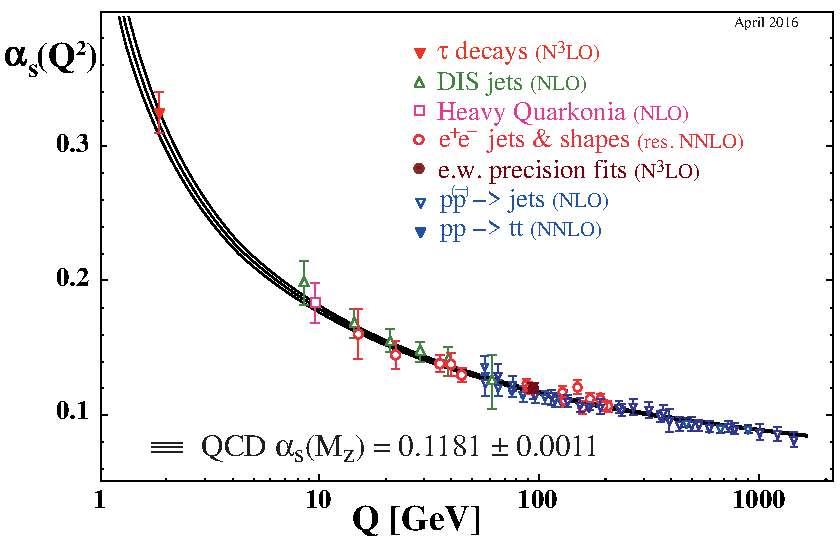
\includegraphics[width=0.8\textwidth]{figures/alpha_s.pdf}
    \caption[Plot of the QCD coupling $\alpha_s$ as a function of energy scale $Q$.]{Plot of the QCD coupling $\alpha_s$ as a function of energy scale $Q$. The respective degree of QCD perturbation theory used in the extraction of $\alpha_s$ is indicated in brackets. Figure taken from Ref.~\cite{PhysRevD.98.030001}.}\label{fig:alpha_s}
\end{figure}

The most successful non-perturbative method thus far for doing calculations in QCD is \emph{Lattice QCD}, which is an \emph{ab initio} method of simulating a discretized version of QCD on a spacetime lattice using Monte Carlo methods. The field of Lattice QCD began with Ken Wilson's famous 1974 paper~\cite{Wilson:1974sk} which showed how to quantize a gauge field theory on a discrete lattice in Euclidean spacetime while preserving exact gauge invariance.

Lattice QCD calculations are very computationally expensive, often requiring hundreds of millions of core hours to perform.~\cite{Fallica2018} In order to ease computational burdens, early calculations used coarse lattices, used very heavy pion masses (which ease the process of inverting very large Dirac matrices), and worked in the so-called ``quenched approximation'' wherein the effects of sea quarks are ignored. Additionally, many (even recent works) ignore the effects of disconnected diagrams in the evaluation of quark propagators, which also amounts to partially ignoring sea-quark effects. The need for an efficient method of performing lattice calculations of fully dynamical QCD neglecting no disconnected contributions has been recently satisfied by the \emph{Stochastic LapH method}~\cite{Morningstar:2011ka}, which is used in this work to study tetraquarks operators in the light scalar sector and the excited $\Sigma$ baryon spectrum. Both of these endeavors are difficult if not impossible to approach without a method such as the Stochastic LapH method, due to disconnected contributions that appear when working with multi-hadron operators that are important in the determination of the excited baryon spectrum and when working with tetraquark operators.

This work is organized as follows. In Chapter~\ref{ch:latticeqcd}, we outline the basic theory underpinning lattice QCD, including how QCD is formulated in discretized spacetime, the path integral approach to calculating observables, and some of the computational details of how our gauge field configurations are generated in such a path integral approach. In Chapter~\ref{ch:operators}, we delve into the details of how to construct quantum operators which create and annihilate the states we wish to study. In Chapter~\ref{ch:montecarlo}, we discuss how to calculate the two-point correlation functions used to extract the energy spectrum, and expound upon how the Stochastic LapH method is used to invert the large Dirac matrices involved in our calculations. In Chapter~\ref{ch:analysis}, we discuss our data analysis procedure which allows us to fit the correlator data we obtain to extract the finite-volume spectrum of QCD. In Chapter~\ref{ch:tetraquarks}, we present results on including tetraquark operators in the sectors containing the $\kappa$ and $a_0(980)$ mesons. In Chapter~\ref{ch:sigmas}, we present results on the excited $\Sigma$ baryon spectrum. Finally, we summarize our results in Chapter~\ref{ch:conclusions}.

\chapter{Lattice QCD}\label{ch:latticeqcd}
\section{QCD in the Continuum}
\subsection{The QCD Lagrangian}
We begin by defining the QCD Lagrangian~\cite{Fritzsch:1973pi} in Euclidean spacetime in terms of quark fields and gluon fields, and discuss the various transformation properties of those fields and the QCD action. As we will see, the advantage of working in Euclidean spacetime is that oscillating exponentials in time become decaying exponentials. This allows us to interpret the Boltzmann factor $e^{-S}$ (where $S$ is the action in Euclidean spacetime) as a probability distribution, allowing us to use Monte Carlo integration to evaluate path integrals in quantum field theory. Additionally, we will see that this gives us access to the low-lying energy spectrum of a theory by allowing us to fit two-point correlation functions to real decaying exponentials. The QCD Lagrangian $\mathcal L_{\rm{QCD}}$ can be written in terms of the fermionic part $\mathcal L_{\rm F}$ and pure-gluon part $\mathcal L_{\rm G}$. In a free theory (i.e.\ without gluons), the fermionic Lagrangian is
\begin{equation}\label{eq:free}
    \mathcal L_{\text{F, free}} = \sum_{f} \overline \psi^{(f)}_{\alpha c}\left((\gamma_\mu)_{\alpha\beta} \partial_\mu + \delta_{\alpha\beta}m^{(f)}\right)\psi^{(f)}_{\beta c}(x),
\end{equation}
where a sum over repeated indices is implied. $\psi$ and $\overline \psi$ are quark and anti-quark fields, respectively, and they carry a flavor index $f$, a Dirac spin index $\alpha$, and a color index $c$. $m^{(f)}$ is the bare mass of the fermion with flavor $f$, and $\gamma_\mu$ are the Euclidean analogs to the familiar Minkowski $\gamma$-matrices satisfying the anticommutation relation $\lbrace\gamma_\mu, \gamma_\nu\rbrace=2\delta_{\mu\nu}\mathbbm 1$, where $\mu\in\lbrace 1,2,3,4\rbrace$ is the Euclidean spacetime index. In its non-interacting form, Eq.~(\ref{eq:free}) appears identical to the familiar QED Lagrangian, except with additional indices for color, which do not mix.

In an interacting theory with gluons, the fermionic part of the Lagrangian becomes
\begin{equation}\label{eq:fermion_lagrangian}
    \mathcal L_{\rm F} = \sum_{f} \overline \psi^{(f)}_{\alpha c}\left((\gamma_\mu)_{\alpha\beta} (\delta_{cd}\partial_\mu + i A_{\mu c d}(x)) + \delta_{\alpha\beta}\delta_{cd} m^{(f)}\right)\psi^{(f)}_{\beta d}(x),
\end{equation}
where we have introduced the gluon fields $A_{\mu c d}$, which carry color indices in addition to spacetime indices. The matrices $A_\mu$ are hermitian and traceless in color space. Being matrices, they make QCD a \emph{non-Abelian} gauge theory, as the gluon fields themselves do not commute. The non-Abelian nature of QCD is the main reason why extracting the low-energy physics is difficult. We define the covariant derivative
\begin{equation}
    D_\mu(x) = \partial_\mu + i A_\mu(x)
\end{equation}
and the field strength tensor
\begin{equation}
    F_{\mu \nu}(x) = -i[D_\mu(x), D_\nu(x)] = \partial_\mu A_\nu(x) - \partial_\nu A_\mu(x) + i[A_\mu(x), A_\nu(x)].
\end{equation}
The gauge fields $A_\mu(x)$ are traceless and hermitian and belong to the Lie algebra $\mathfrak{su}$(3). Therefore, we can write $A_\mu$ in terms of the 8 generators of SU(3), denoted by $T_i$, which form a basis for $\mathfrak{su}$(3), as
\begin{equation}
    A_{\mu}(x)=\sum_{i=1}^{8} A_{\mu}^{(i)}(x) T_{i}.
\end{equation}
We call $A_{\mu}^{(i)}(x)$ the \emph{color components} of the gauge field, and they are real-valued. The generators satisfy the following properties in addition to being traceless, complex, and hermitian:
\begin{equation}
    \tr \left[T_{j} T_{k}\right]=\frac{1}{2} \delta_{j k}
\end{equation}
and
\begin{equation}
    \left[T_{j}, T_{k}\right]=\mathrm{i} f_{j k l} T_{l},
\end{equation}
where $f_{jkl}$ are known as the \emph{structure constants} and are completely anti-symmetric. Conventionally, we choose to represent $\mathfrak{su}$(3) using $T_a = \frac{\lambda_a}{2}$, where $\lambda_a$ are the Gell-Mann matrices~\cite{GellMann:1962xb}.

Now we write down the gluonic part of the QCD Lagrangian,
\begin{equation}\label{eq:Lg}
    \mathcal L_{\rm G} = \frac{1}{2g^2} \tr[F_{\mu\nu}(x) F_{\mu\nu}(x)],
\end{equation}
where $g$ is the QCD coupling parameter. Using the decomposition of the gluon fields into their color components, we can similarly decompose the field strength tensor into its color components to gain more insight into the gluonic part of the Lagrangian:
\begin{equation}
    \begin{aligned}
        F_{\mu \nu}(x) &=\sum_{i=1}^{B} F_{\mu \nu}^{(i)}(x) T_{i}, \\
        F_{\mu \nu}^{(i)}(x) &=\partial_{\mu} A_{\nu}^{(i)}(x)-\partial_{\nu} A_{\mu}^{(i)}(x)-f_{i j k} A_{\mu}^{(j)}(x) A_{\nu}^{(k)}(x).
        \end{aligned}
\end{equation}
Plugging this into Eq.~(\ref{eq:Lg}), we find that the QCD Lagrangian contains 3- and 4-vertex gluonic self-interactions. This makes QCD and QED fundamentally different: in QED we have linear superposition since the massless vector boson (the photon) does not self-interact, whereas in QCD, linear superposition never applies due to the gluon self-interactions.
\subsection{Transformation Properties of the Quark and Gluon Fields}
QCD is an SU(3) gauge theory, meaning the action is invariant under local SU(3) gauge transformations of the quark and gluon fields. Such a gauge transformation can be associated with a $3\times3$ unitary color-space transformation $\Omega(x)$ at each spacetime point $x$, which also has the property $\det[\Omega(x)] = 1$. In order to ensure gauge invariance, we demand that the quark fields transform as
\begin{equation}\label{eq:quark_transf}
    \begin{aligned}
    \psi(x) &\rightarrow \psi^{\prime}(x)=\Omega(x) \psi(x)\\
    \overline{\psi}(x) &\rightarrow \overline{\psi}^{\prime}(x)=\overline{\psi}(x) \Omega(x)^{\dagger},
    \end{aligned}
\end{equation}
and the gluon fields transform as
\begin{equation}\label{eq:gluon_transf}
    A_{\mu}(x) \rightarrow A_{\mu}^{\prime}(x)=\Omega(x) A_{\mu}(x) \Omega(x)^{\dagger}+\mathrm{i}\left(\partial_{\mu} \Omega(x)\right) \Omega(x)^{\dagger},
\end{equation}
where we have suppressed Dirac indices and used matrix/vector notation for the color indices. One can then verify that Eqs.~(\ref{eq:quark_transf}) and (\ref{eq:gluon_transf}) leave the action $S=\int d^4 x \lbrace \mathcal L_{\rm{F}} + \mathcal L_{\rm{G}}\rbrace$ invariant.
\section{Discretizing QCD on the Lattice}
To facilitate our nonperturbative computations, we must formulate QCD on a spacetime lattice. We consider our lattice $\Lambda$ as an isotropic four-dimensional grid of points, indexed by a 4-tuple of integers $n$ such that $x=an$, where $a$ is the lattice spacing. That is, we can write
\begin{equation}
    \Lambda = \lbrace n = (n_1, n_2, n_3, n_4)\rbrace,
\end{equation}
where $n_i$ are integers. We will later also consider anisotropic lattices. Since a lattice has finite spacing, that implies a momentum cutoff, which also acts as an ultraviolet regulator for the theory. That is, the $i$ component momentum is restricted to $p_i \in (-\frac{\pi}{a}, \frac{\pi}{a}]$. Additionally, we will work with periodic boundary conditions, which discretizes the momentum $\bs p = \frac{2\pi \bs n}{L}$, where $\bs n$ is a vector of integers and $L$ is the length of the lattice. 
\subsection{Free Fermions}
We begin with a naive approach to discretizing fermions on the lattice, which will then be improved upon. The continuum action for one free fermion with a bare mass $m$ can be written as
\begin{equation}\label{eq:action_ff}
    S_{F}^{0}[\psi, \overline{\psi}]=\int d^{4} x \; \overline{\psi}(x)\left(\gamma_{\mu} \partial_{\mu}+m\right) \psi(x).
\end{equation}
A first pass at discretizing Eq.~(\ref{eq:action_ff}) involves replacing the integral by a sum, replacing $x$ by $n$, and rewriting the derivative terms as simple finite differences, like so,
\begin{gather}
    \int d^4x \rightarrow a^4 \sum_n \\
    \psi(x) \rightarrow \psi(n) \\
    \overline\psi(x) \rightarrow \overline\psi(n) \\
    \partial_{\mu} \psi(x) \rightarrow \frac{1}{2 a}(\psi(n+\hat{\mu})-\psi(n-\hat{\mu})).
\end{gather}
We immediately find that such a discretization scheme breaks local SU(3) gauge invariance, due to terms of the form $\overline\psi(n) \psi(n+\hat\mu)$.
\subsection{Gauge Fields and Link Variables}
Though we expect that gauge invariance for the free fermion action is restored in the limit $a \rightarrow 0$, we wish to maintain exact gauge invariance for finite $a$ in the entire discretized action. In determining how to discretize the gluon fields, we are guided by this requirement. Under a local gauge transformation $\Omega(n)$,
\begin{equation}
    \overline{\psi}(n) \psi(n+\hat{\mu}) \rightarrow \overline{\psi}(n) \Omega(n)^{\dagger} \Omega(n+\hat{\mu}) \psi(n+\hat{\mu}),
\end{equation}
which is obviously not gauge-invariant. We can fix this issue by introducing new fields $U_\mu(n)$, called \emph{link variables}~\cite{Wilson:1974sk}, which transform under a gauge transformation as
\begin{equation}\label{eq:link_transf}
    U_{\mu}(n) \rightarrow \Omega(n) U_{\mu}(n) \Omega(n+\hat{\mu})^{\dagger}.
\end{equation}
These link variables are matrix-valued, and are elements of the gauge group SU(3). They are also directionally oriented, and are defined such that $U_{-\mu}(n) \equiv U_{\mu}(n-\hat{\mu})^{\dagger}$. They can be visually represented as living on the links between lattice sites, as depicted in Fig.~\ref{fig:links}.
\begin{figure}
    \centering
    % 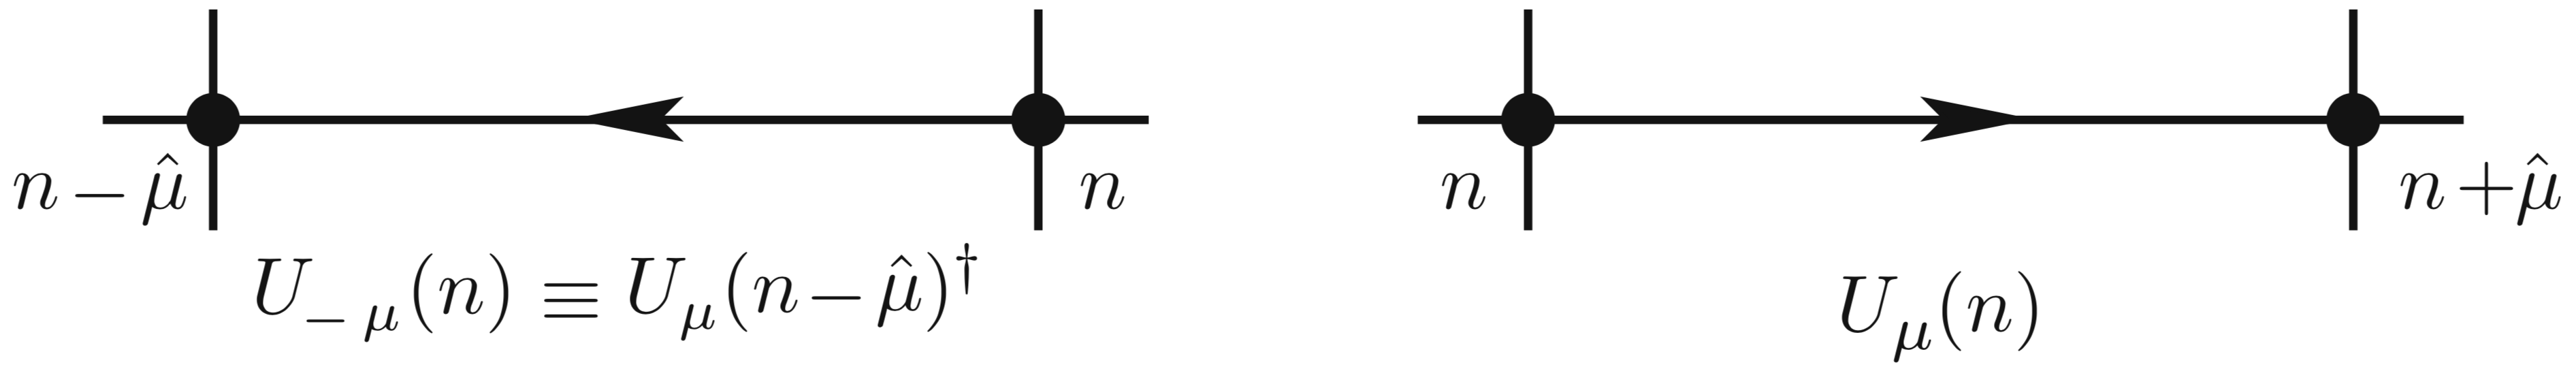
\includegraphics[scale=0.2]{figures/links.png}
    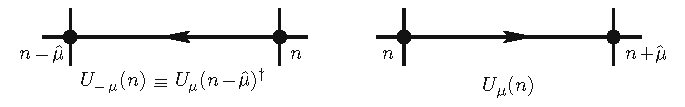
\includegraphics[width=0.7\textwidth]{figures/links.pdf}
    \caption{Link variables, depicted as linking two adjacent lattice sites.}
    \label{fig:links}
\end{figure}
We then propose the following form for the naively discretized interacting fermionic action for one flavor as follows, which one can verify to be gauge-invariant:
\begin{equation}\label{eq:lattice_fermion_action}
    S_{F}[\psi, \overline{\psi}, U]=a^{4} \sum_{n \in A} \overline{\psi}(n)\left(\sum_{\nu=1}^{4} \gamma_{\mu} \frac{U_{\mu}(n) \psi(n+\hat{\mu})-U_{-\mu}(n) \psi(n-\hat{\mu})}{2 a}+m \psi(n)\right).
\end{equation}
In taking the limit $a\rightarrow 0$, the fermionic action will contain $\mathcal O(a)$ lattice artifacts. Now that we have identified a candidate for a gauge-invariant discretized interacting fermion action, it remains to relate the link variables $U_\mu(n)$ to the continuum gauge fields $A_\mu(x)$. In the continuum, there is an object which satisfies the same gauge transformation properties as the link variables (see Eq.~(\ref{eq:link_transf})), and that object is the gauge transporter,
\begin{equation}
    G(x, y)=P \exp \left(\mathrm{i} \int_{\mathcal{C}_{x y}} A \cdot d s\right),
\end{equation}
where $C_{xy}$ is a curve connecting two points $x$ and $y$, and $P$ denotes path-ordering. The link variables approximate this gauge transporter, i.e.\ $U_\mu(n) = G(n, n+\hat \mu) + \mathcal O(a)$, and are given by
\begin{equation}
    U_{\mu}(n)=\exp \left(\mathrm{i} a A_{\mu}(n)\right).
\end{equation}
One can verify that in the continuum limit $a\rightarrow 0$, the action in Eq.~(\ref{eq:lattice_fermion_action}) reduces to its continuum form given by integrating the Lagrangian in Eq.~(\ref{eq:fermion_lagrangian}). Note that we have gone from using $\mathfrak{su}(3)$ Lie algebra-valued fields $A_\mu(x)$ to variables $U_\mu(x)$ which are elements of the Lie group SU(3). This will become relevant in defining the path integral on the lattice.
\subsection{Fermion Doubling}
We define the \emph{Dirac Matrix} $M[U]$ for a theory with one fermion flavor by rewriting the fermion action in Eq.~(\ref{eq:lattice_fermion_action}) as
\begin{equation}
    S_F[\psi, \overline \psi, U] = \sum_{n,m\in \Lambda} \sum_{a,b,\alpha,\beta} \overline \psi(n)_{\alpha a} M(n|m)_{\alpha\beta;a b} \psi(m)_{\beta b},
\end{equation}
implying that
\begin{equation}
    M(n | m)_{\alpha \beta; a b} = a^4\sum_{\mu=1}^{4}\left(\gamma_{\mu}\right)_{\alpha \beta} \frac{U_{\mu}(n)_{a b} \delta_{n+\hat{\mu}, m}-U_{-\mu}(n)_{a b} \delta_{n-\hat{\mu}, m}}{2 a}+m \delta_{\alpha \beta} \delta_{a b} \delta_{ m}.
\end{equation}
The free quark propagator on the lattice is found by inverting the Dirac matrix when the gauge fields are set to $U_\mu(n) = \mathbbm 1$. In momentum space, the Dirac matrix is given by
\begin{equation}\label{eq:ms_dirac}
    \widetilde{M}(p)=a^4 \left(m + i \sum_{\mu=1}^{4} \gamma_{\mu} \frac{\sin \left(p_{\mu} a\right)}{a}\right)
\end{equation}
and its inverse is
\begin{equation}
    \widetilde M^{-1}(n|m) = a^{-4}\frac{m - ia^{-1}\sum_\mu \gamma_\mu \sin(p_\mu a)}{m^2 + a^{-2}\sum_\mu\sin(p_\mu a)^2}.
\end{equation}
If we examine this propagator in the massless case, $m=0$, we find a pole at $p^2 = 0$, as we would expect. However, we also find 15 additional poles at the corners of the first Brillouin zone, i.e.\ at $p=(\pi / a, 0,0,0),(0, \pi / a, 0,0), \ldots,(\pi / a, \pi / a, \pi / a, \pi / a)$. These extra poles are known as the \emph{doublers}. They are not present in the continuum (just take $a\rightarrow 0$ in the denominator of the propagator to see this), but on the lattice, we must deal with these unphysical poles. Wilson found a clever way to deal with these doublers~\cite{Wilson:1975id} by adding an additional term, now known as the \emph{Wilson term}, to the Dirac matrix. In momentum space, the Dirac matrix with the added Wilson term is (c.f. Eq.~(\ref{eq:ms_dirac}))
\begin{equation}
    \widetilde{M}(p)=a^4\left(m +i \sum_{\mu=1}^{4} \gamma_{\mu} \frac{\sin \left(p_{\mu} a\right)}{a}+ \sum_{\mu=1}^{4}\frac{\left(1-\cos \left(p_{\mu} a\right)\right)}{a}\right).
\end{equation}
The Wilson term vanishes at $p=(0,0,0,0)$, but acts as an extra mass term at each corner of the Brillioun zone. These mass terms scale as $\frac{1}{a}$, so for small lattices, they will decouple from the theory and not affect the low energy spectrum. Inverting the Fourier transform, the Wilson term turns out to be a discretization of $-\frac{a}{2}\partial_\mu \partial_\mu$, which vanishes in the continuum limit.

While the Wilson term solves our fermion doubling problem, it introduces a new problem. Since the Wilson term is proportional to $\mathbbm 1$ in Dirac space, it does not anticommute with $\gamma_5 = \gamma_4 \gamma_1 \gamma_2 \gamma_3$, which implies that it violates chiral symmetry. (See Section 7.2 in Ref.~\cite{Gattringer:2010zz} for more details.) This problem of chiral symmetry breaking is not a defect of only Wilson's solution to fermion doubling, but of any solution that attempts to add terms to free the theory of doublers, as shown in the famous ``no-go'' theorem of Nielson and Ninomiya~\cite{Nielsen:1981hk}.
\subsection{The Wilson Gauge Action}
After constructing a discretized version of the fermion action, it remains to construct a discretized version of the gauge action. The first step is to identify a gauge-invariant object constructed only of link variables. An ordered product of link variables
\begin{equation}
    P[U]=U_{\mu_{0}}\left(n_{0}\right) U_{\mu_{1}}\left(n_{0}+\hat{\mu}_{0}\right) \ldots U_{\mu_{k-1}}\left(n_{1}-\hat{\mu}_{k-1}\right) \equiv \prod_{(n, \mu) \in \mathcal{P}} U_{\mu}(n)
\end{equation}
along a path $\mathcal P$ on the lattice is the lattice analog to the continuum gauge transporter. This product shares the same transformation properties as the link variables and the continuum gauge transporter, i.e.\
\begin{equation}
    P[U] \rightarrow \Omega\left(n_{0}\right) P[U] \Omega\left(n_{1}\right)^{\dagger}.
\end{equation}
If we choose a path that forms a closed loop $\mathcal L$, then such a product transforms under a gauge transformation as
\begin{equation}\label{eq:loop}
    \prod_{(n, \mu) \in \mathcal{L}} U_{\mu}(n) \rightarrow \Omega\left(n_{0}\right) \prod_{(n, \mu) \in \mathcal{L}} U_{\mu}(n) \Omega\left(n_{0}\right)^{\dagger},
\end{equation}
since the color rotations $\Omega(n)$ cancel out at every intermediate point due to unitary. We can then use the cyclicity of the trace to form a gauge-invariant object out of Eq.~(\ref{eq:loop}). Hence,
\begin{equation}
    \tr[\prod_{(n, \mu) \in \mathcal{L}} U_{\mu}(n)]
\end{equation}
is gauge-invariant. The shortest closed loop is called the \emph{plaquette}, which is defined as a product of four link variables,
\begin{equation}
    U_{\mu \nu}(n)=U_{\mu}(n) U_{\nu}(n+\hat{\mu}) U_{-\mu}(n+\hat{\mu}+\hat{\nu}) U_{-\nu}(n+\hat{\nu}).
\end{equation}
With these definitions, we now write down Wilson's formulation of the gauge action on the lattice, which is a sum over all possible plaquettes on the lattice (only counting one orientation for each plaquette):
\begin{equation}
    S_{G}[U]=\frac{2}{g^{2}} \sum_{n \in \Lambda} \sum_{\mu<\nu} \operatorname{Re}\,\operatorname{tr}\left[\mathbbm{1}-U_{\mu \nu}(n)\right].
\end{equation}
In the continuum limit $a\rightarrow 0$, it can be shown that this reduces to the continuum version given by integrating the Lagrangian in Eq.~(\ref{eq:Lg}). In taking the limit, the action will contain $\mathcal O(a^2)$ lattice artifacts, that is,
\begin{equation}
    S_{G}[U]=\frac{2}{g^{2}} \sum_{n \in \Lambda} \sum_{\mu<\nu} \operatorname{Re} \operatorname{tr}\left[\mathbbm{1}-U_{\mu \nu}(n)\right]=\frac{a^{4}}{2 g^{2}} \sum_{n \in A} \sum_{\mu, \nu} \operatorname{tr}\left[F_{\mu \nu}(n)^{2}\right]+\mathcal{O}\left(a^{2}\right).
\end{equation}
The Wilson action is just one way to formulate a discretized gauge action. We will discuss different discretization strategies in order to reduce the discretization error to higher orders in $a$.
\subsection{Improving the Discretized Action}\label{sec:improved_action}
In our naively discretized theory, the fermionic action action contains $\mathcal O(a)$ lattice artifacts and the gauge action contains $\mathcal O(a^2)$ artifacts. By adding terms to the action which cancel these artifacts but which vanish in the continuum limit, we can improve discretization errors to higher orders in $a$. This is called \emph{Symanzik improvement}~\cite{Symanzik:1983dc}. For example, we make use of a \emph{clover improved}~\cite{Sheikholeslami:1985ij} action, which involves adding a term to the Wilson action,
\begin{equation}
    c_{\mathrm{sw}} a^{5} \sum_{n \in \Lambda} \sum_{\mu<\nu} \bar{\psi}(n) \frac{1}{2} \sigma_{\mu \nu} \widehat{F}_{\mu \nu}(n) \psi(n),
\end{equation}
where $c_{\mathrm{sw}}$ is a real coefficient, called the Sheikholeslami-Wohlert coefficient,
\begin{equation}
    \widehat{F}_{\mu \nu}(n)=\frac{-\mathrm{i}}{8 a^{2}}\left(Q_{\mu \nu}(n)-Q_{\nu \mu}(n)\right),
\end{equation}
\begin{equation}
    \sigma_{\mu \nu} \equiv\left[\gamma_{\mu}, \gamma_{\nu}\right] / 2 \mathrm{i},
\end{equation}
and
\begin{equation}
    Q_{\mu \nu}(n) \equiv U_{\mu, \nu}(n)+U_{\nu,-\mu}(n)+U_{-\mu,-\nu}(n)+U_{-\nu, \mu}(n).
\end{equation}
The clover term is named as such because it is constructed from four adjacent plaquettes, as depicted in Fig.~\ref{fig:clover}.
\begin{figure}
    \centering
    % 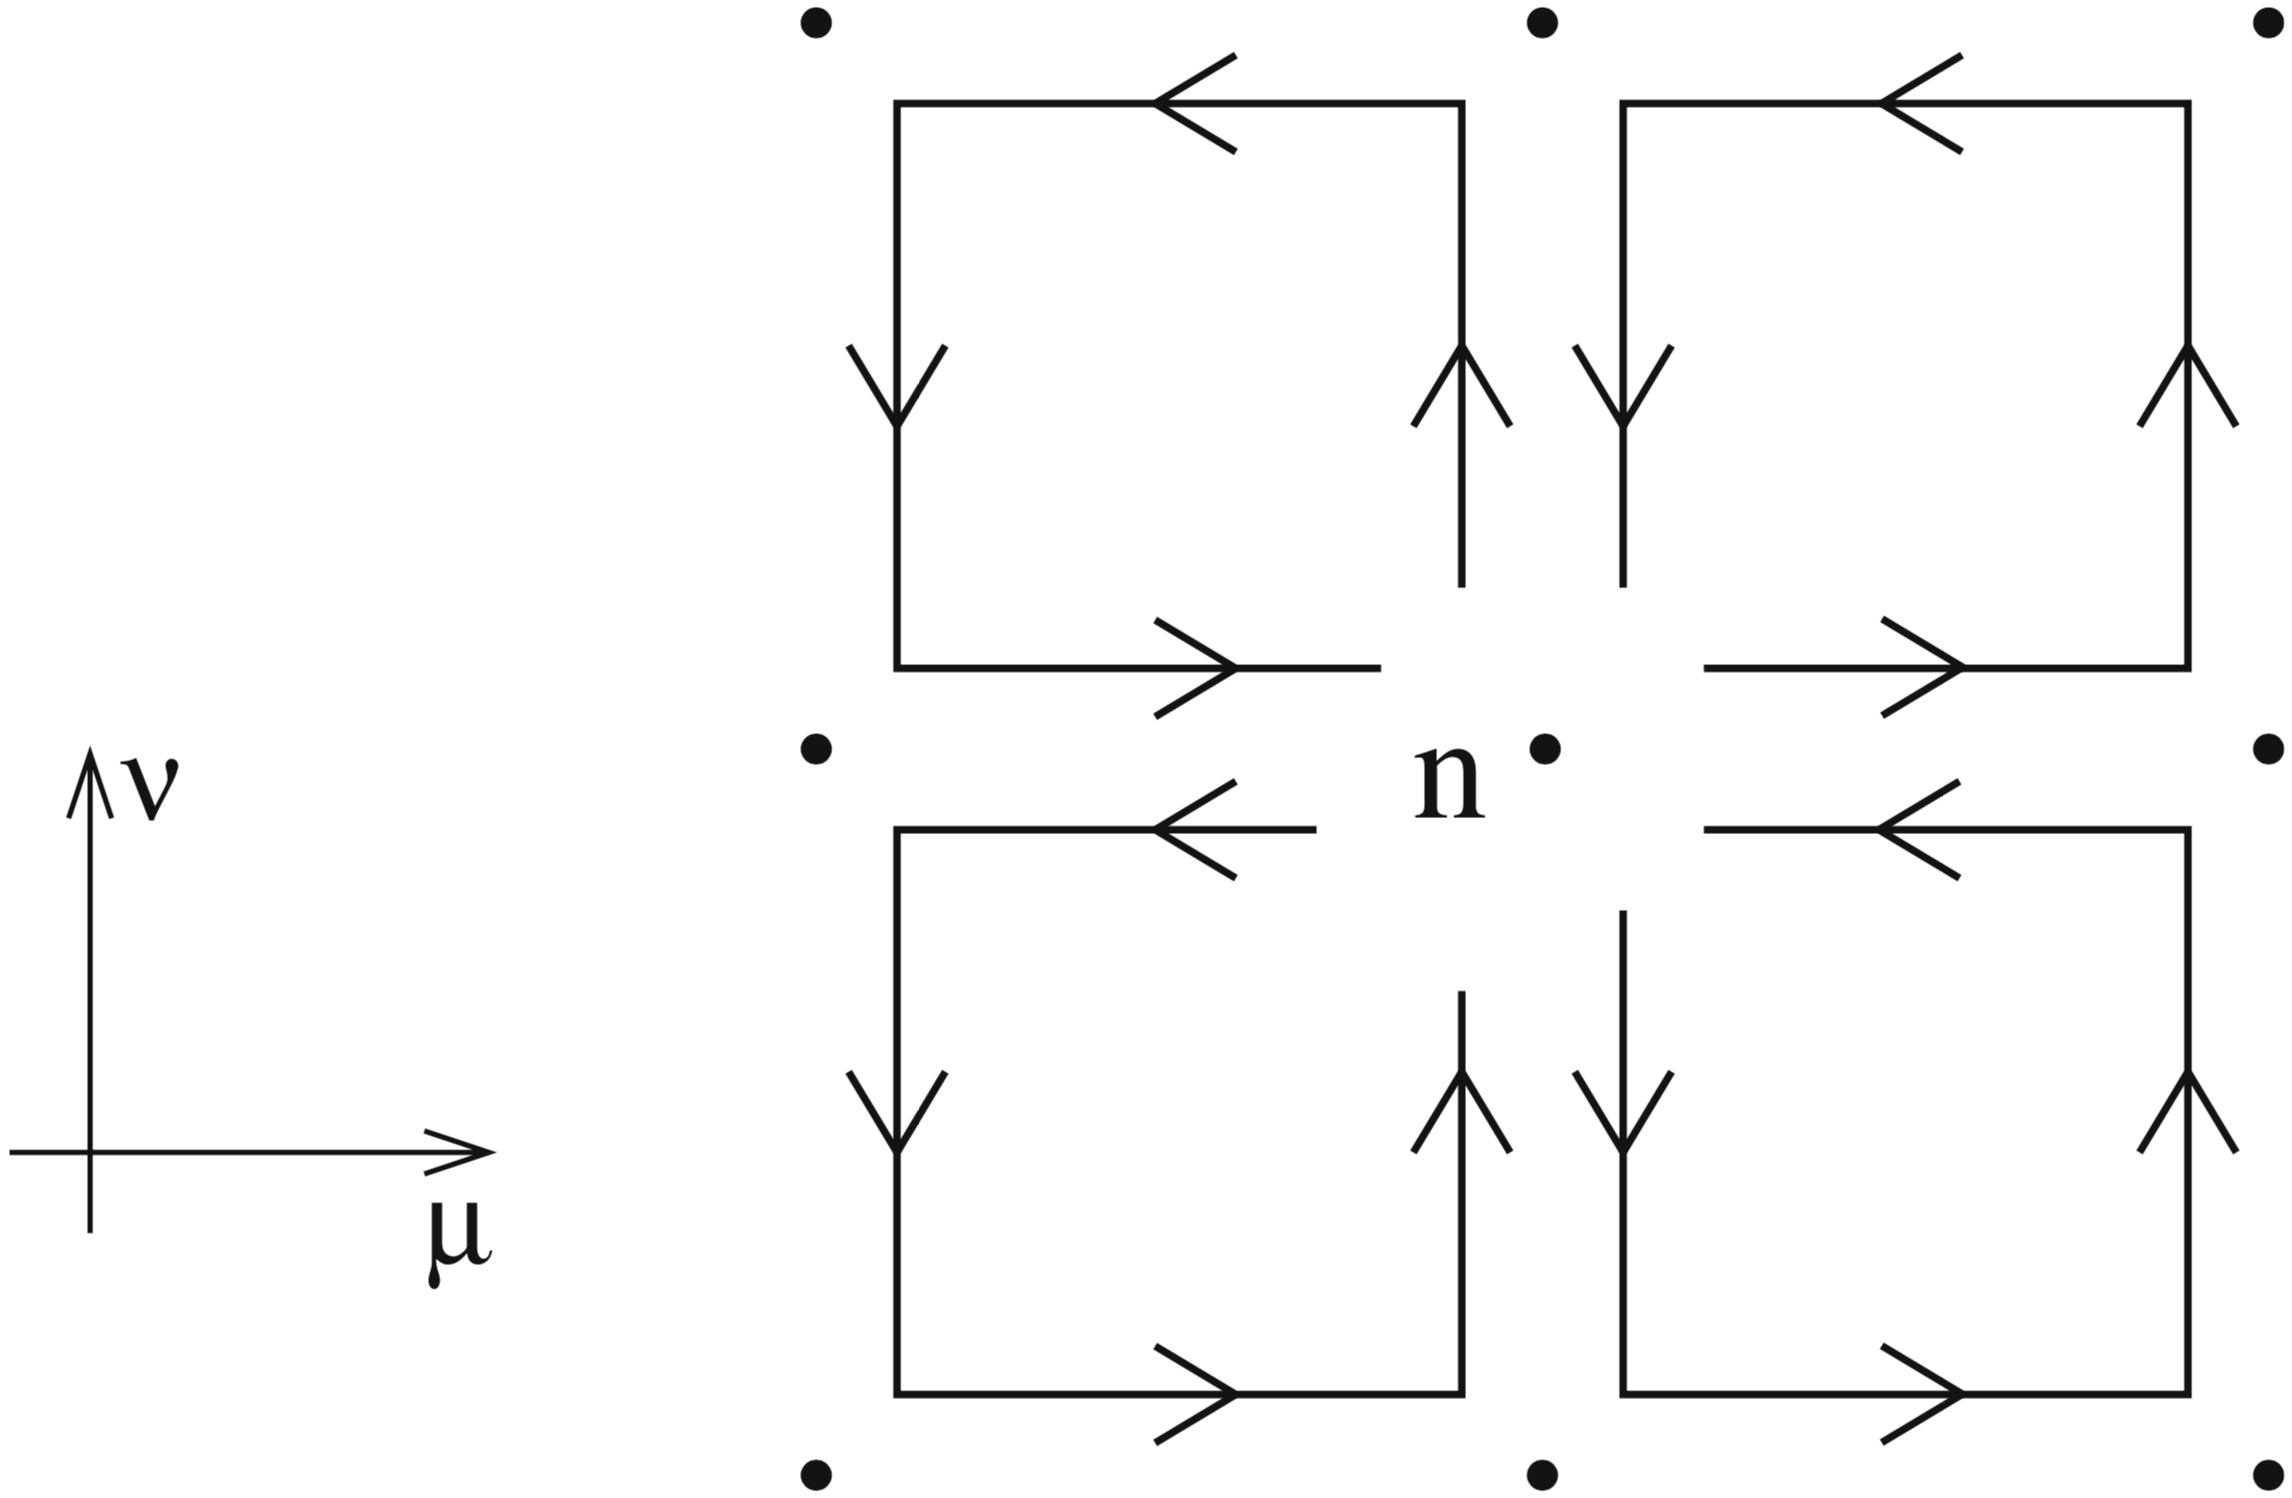
\includegraphics[scale=0.2]{figures/clover.png}
    \hspace*{-1in}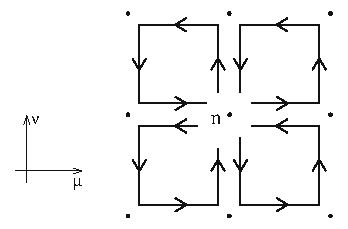
\includegraphics[width=0.6\textwidth]{figures/clover.pdf}
    \caption{Depiction of the clover term, built out of four plauqettes.}
    \label{fig:clover}
\end{figure}

In addition to Symanzik improvements, there are so-called \emph{tadpole} improvements~\cite{Lepage:1992xa} that can be made to the gauge action. These seek to correct contributions from QCD tadpole diagrams that appear at low energy, when the coupling is large. For a small coupling $g$, we may reasonably expand the link variables as $U_{\mu}(x) \equiv e^{i a g A_{\mu}(x)} \rightarrow 1+i a g A_{\mu}(x)$. It turns out, however, that higher order terms are suppressed by powers of $g^2$, and so when the coupling is large, there will be contributions from QCD tadpoles. For a detailed presentation, see~\cite{Lepage:1992xa}. In order to deal with these tadpoles, we rescale the link variables as $U \rightarrow \frac{U}{u}$, where
\begin{equation}
    u=\left\langle\frac{1}{3} \operatorname{Re} \operatorname{Tr} U_{\mu \nu}\right\rangle^{1 / 4}.
\end{equation}
$u$ is both a parameter of the action and an observable, so we must iteratively tune $u$ in the action such that the $u$ we observe is the same as the $u$ we put into the action.

In practice, our lattices are anisotropic~\cite{Edwards:2008ja, Lin:2008pr}. The motivation for this is that the primary observables we measure are temporal correlators whose signal-to-noise ratios decrease as time separation increases. To combat this issue, we could use a finer lattice in order to sample the correlators at more time separations. The computational cost of refining the lattice in every direction is large, however, so we choose to refine only the temporal direction. That is, we choose an anisotropy $\xi \equiv \frac{a_s}{a_t} > 1$, where $a_s$ is the spatial lattice spacing and $a_t$ is the temporal lattice spacing. $\xi$ is in fact a quantity that undergoes renormalization, so the anisotropy enters into the gauge action as a parameter $\gamma_g$ and into the fermionic action as a parameter $\gamma_f$. Both of these parameters must be tuned to produce the desired renormalized anisotropy.

Finally, we write down the action we use in this work. The gauge action is a Symanzik-improved L\"uscher-Weisz action~\cite{Luscher:1984xn,Luscher:1985zq}, and uses tadpole improvement coefficients from~\cite{Morningstar:1997ff, Morningstar:1999rf, Lin:2008pr,Edwards:2008ja}:
\begin{equation}
    S_{G}^{\xi}[U]=\frac{\beta}{3 \gamma_{g}}\left[\sum_{x, i \neq j}\left(\frac{5}{6 u_{s}^{4}} \Omega_{\mathcal{P}_{i j}}(x)-\frac{1}{12 u_{s}^{6}} \Omega_{\mathcal{R}_{i j}}(x)\right)+\sum_{x, i}\left(\frac{4}{3 u_{s}^{2} u_{t}^{2}} \Omega_{\mathcal{P}_{i t}}(x)-\frac{1}{12 u_{s}^{4} u_{t}^{2}} \Omega_{\mathcal{R}_{i t}}\right)\right].
\end{equation}
Here, $P$ is a plaquette, $\Omega_P = \Re \Tr(1-P)$, $R$ is a $2\times 1$ planar Wilson loop, $u_s$ and $u_t$ are the aforementioned tadpole improvement coefficients, $\beta$ is the inverse gauge coupling, and $\gamma_g$ is the bare anisotropy parameter for the gauge sector. Notice that only improvements in spatial links have been included. Lattice gauge-field actions which involve more than two time slices often lead to temporal correlators which do not fall exponentially in a simple way. This action has $\mathcal O(a_s^4, a_t^2, g^2a_s^2)$ discretization errors. The fermionic part of the action is given by
\begin{equation}
    \begin{aligned}
        S_{F}^{\xi}[U, \bar{\psi}, \psi] &=\sum_{x} \overline{\hat{\psi}}(x) \frac{1}{\tilde{u}_{t}}\left\{\tilde{u}_{t} \hat{m}_{0}+\gamma_{t} \hat{W}_{t}+\frac{1}{\gamma_{f}} \sum_{s} \gamma_{s} \hat{W}_{s}\right.\\
        &\left.-\frac{1}{2}\left[\frac{1}{2}\left(\frac{\gamma_{g}}{\gamma_{f}}+\frac{1}{\xi}\right) \frac{1}{\tilde{u}_{t} \tilde{u}_{s}^{2}} \sum_{s} \sigma_{t s} \hat{F}_{t s}+\frac{1}{\gamma_{f}} \frac{1}{\tilde{u}_{s}^{3}} \sum_{s<s^{\prime}} \sigma_{s s^{\prime}} \hat{F}_{s s^{\prime}}\right]\right\} \hat{\psi}(x).
        \end{aligned}
\end{equation}
Here, $\gamma_f$ is the bare anisotropy for the gauge sector, $\xi = \frac{a_s}{a_t}$ is the renormalized anisotropy, $\gamma_\mu$ and $\sigma_{\mu\nu} = \frac{1}{2}[\gamma_\mu, \gamma_\nu]$ are Dirac gamma matrices, $\tilde u_s$ is the spatial tadpole improvement factor, and $\tilde u_t$ is the temporal tadpole improvement factor. Hats denote dimensionless quantities that relate to dimensionful quantities by scaling with appropriate factors of the lattice spacing. $\hat{\psi}=a_{s}^{3 / 2} \psi$ where $\psi$ is the quark field, $\hat{m}_{0}=m_{0} a_{t}$ where $m_0$ is the bare quark mass, and $\hat{F}_{\mu \nu}=a_{\mu} a_{\nu} F_{\mu \nu}=\frac{1}{4} \operatorname{Im}\left(\mathcal{P}_{\mu \nu}(x)\right)$ where $F_{\mu\nu}$ is the field strength tensor. $\hat W$ is the \emph{Wilson operator}, and is given by
\begin{equation}
    \hat{W}_{\mu} \equiv \hat{\nabla}_{\mu}-\frac{1}{2} \gamma_{\mu} \hat{\Delta}_{\mu},
\end{equation}
where
\begin{equation}
    \hat{\nabla}_{\mu}=a_{\mu} \nabla_{\mu},\; \hat{\Delta}_{\mu}=a_{\mu}^{2} \Delta_{\mu}.
\end{equation}
This action has $\mathcal{O}\left(g^{2} a_{s}, g^{2} a_{t}, a_{s}^{2}, a_{t}^{2}\right)$ discretization errors. It is also important to mention that the link variables in the fermionic action are \emph{stout-smeared}~\cite{Morningstar:2003gk}, which we will discuss further in Chapter~\ref{ch:operators}. The use of smeared link variables in the action leads to better chiral behavior.
\subsection{Parameter Tuning}\label{sec:tuning}
\subsubsection{Anisotropy}
The parameters we put into our action are bare parameters. We obtain these parameters by choosing a set of observables, and tuning the bare parameters in our action such that their desired values are produced. For example, we desire a renormalized anisotropy $\xi\approx 3.5$, and must tune the values $\gamma_g$ and $\gamma_f$ to obtain this. In order to tune $\gamma_g$, we measure the following quantities~\cite{Klassen:1998ua}:
\begin{equation}
    \begin{aligned}
        R_{s s}(x, y)&=\frac{W_{s s}(x, y)}{W_{s s}(x+1, y)},\\
        R_{s t}(x, t)&=\frac{W_{s t}(x, t)}{W_{s t}(x+1, t)},
    \end{aligned}
\end{equation}
where $W_{\mu\nu}(x_\mu, x_\nu)$ is the expectation value of a Wilson loop of size $x_\mu$ and $x_\nu$ and oriented in the $\mu$ and $\nu$ directions, and then demand that $R_{s s}(x, y)=R_{s t}(x, \xi t)$.  In order to tune $\gamma_f$, we impose a continuum dispersion relation for mesons on the lattice,
\begin{equation}
    a_{t}^{2} E^{2}(\boldsymbol{p})=a_{t}^{2} m^{2}+\frac{a_{s}^{2} \boldsymbol{p}^{2}}{\xi^{2}}.
\end{equation}
We find that in order to attain $\xi\approx 3.5$, we set $\gamma_g = 4.3$ and $\gamma_f = 3.4$.
\subsubsection{Gauge Coupling and Lattice Spacing}
The renormalization scheme we use requires that the coupling and masses in the lattice QCD action vary (or run) with the ultraviolet cutoff such that observables tend to their physical values as the cutoff is removed. The lattice spacing acts as a cutoff by eliminating very small wavelengths from the theory.  The cutoff is proportional to the inverse lattice spacing, limiting momenta to the first Brillouin zone. We tune the inverse coupling $\beta$ in our action to obtain a desired lattice spacing. Determining the lattice spacing using a physical observable is known as \emph{setting the scale}. One way to set the scale is by choosing a particle, say the $\Omega$, and requiring that its mass measured on the lattice should equal its physical mass. That is, we calculate
\begin{equation}
    a_t = \frac{a_t m}{m_{\rm{Phys}}},
\end{equation}
where $a_t m$ is the quantity we directly measure in a lattice calculation. In our calculations, this yields $a_t\approx 0.034$ fm, giving $a_s\approx 0.12$ fm, and we obtain these values by choosing $\beta = 1.5$.
\subsubsection{Quark Masses}
As we will discuss further in Chapter~\ref{ch:operators}, we work in a theory of $N_f=2+1$ QCD, meaning there are three flavors of quarks, two of which have degenerate masses. These are the degenerate up and down quarks (collectively referred to as the \emph{light} quarks), and the strange quark. An important flaw of our calculations is that we work in a theory of an unphysically heavy pion. This is necessary for two reasons. First, finite volume corrections to the theory are exponentially suppressed by a factor of $e^{-m_\pi L}$, where $m_\pi$ is the mass of the pion (in general, it is the mass of the lightest state in the theory) and $L$ is the spatial extent of the lattice. It is necessary that the \emph{correlation length}, $m_\pi L$ is $>1$, but in practice, a good rule of thumb is to require $m_\pi L > 4$ or so. Second, inverting Dirac matrices (which we will soon see to be an important step of our calculation) becomes much more computationally difficult at lower pion masses, and increases the odds that the Dirac matrices will become ill-conditioned.

In order to tune the light and strange quark masses, we aim to set the following ratios to their physical values~\cite{Lin:2008pr}:
\begin{equation}
        l_{\Omega}=\frac{9 m_{\pi}^{2}}{4 m_{\Omega}^{2}},\quad
        s_{\Omega}=\frac{9\left(m_{K}^{2}-m_{\pi}^{2}\right)}{4 m_{\Omega}^{2}},
\end{equation}
where $m_K$ is the mass of the kaon, $m_\pi$ is the mass of the pion, and $m_\Omega$ is the mass of the $\Omega$ baryon. These ratios are chosen because first-order chiral perturbation theory tells us that they should be proportional to their associated quark masses~\cite{Lin:2008pr}. $s_\Omega$ is set to its physical value, and $l_\Omega$ is lowered to a value 
that is unphysical but allows calculations to remain possible. Using this method of tuning, the bare quark masses are set to be $a_t m_l = -0.0860$ for the light quarks, 
and $a_t m_s = -0.0743$ for the strange quark. With these quark masses, our pion mass is 
approximately 230 MeV.

\section{Extracting Energies from Two-Point Correlation Functions}\label{sec:intro_corr}
In order to do spectroscopy, the main observables we calculate on the lattice are time-ordered two-point correlation functions of the form
\begin{equation}
    C(t) = \bra 0 \mathcal O (t+t_0) \overline{\mathcal O}(t_0) \ket 0,
\end{equation}
where $\ket 0$ is the vacuum state, $\overline{\mathcal O}(t_0)$ is an operator that creates a state out of the vacuum at time $t_0$, and $\mathcal O (t+t_0)$ is an operator that annihilates such a state at a later time $t+t_0$. Let $\ket n$ denote the $n^{\rm{th}}$ energy eigenstate of the theory with energy $E_n$, ordered such that $E_n < E_{n+1}$, and let us shift the energies such that the vacuum energy $E_0 \equiv 0$. Then, using a spectral decomposition and working in the Heisenberg picture in imaginary time $t\rightarrow -it$, we can see
\begin{equation}\label{eq:corr_decomp}
    \begin{aligned}
        C(t) &= \sum_{n=0}^\infty \bra 0 e^{H(t+t_0)} \mathcal O(0) e^{-H(t+t_0)} \ket n \bra n e^{H t_0} \overline{\mathcal O}(0)e^{-H t_0} \ket 0 \\
        &=\sum_{n=0}^\infty e^{E_0(t+t_0)} \bra 0 \mathcal O(0) \ket n e^{-E_n(t+t_0)} e^{E_n t_0} \bra n \overline{\mathcal O}(0) \ket 0 e^{-E_0 t_0}\\
        & = \sum_{n=0}^\infty \bra 0 \mathcal O(0) \ket n \bra n \overline{\mathcal O}(0)\ket 0 e^{-E_n t}.
    \end{aligned}
\end{equation}
Here, we have made the assumption that $t \ll T$, where $T$ is the temporal length of the lattice, which is necessary to prevent temporal wrap-around effects. It is now clear that by calculating $C(t)$ on the lattice, we have access to the energy spectrum of the theory. In principle, with infinite statistics, we could fit $C(t)$ to obtain the entire spectrum. In practice, however, we can only reliably extract the lowest non-zero energy in this sum by fitting $C(t)$ to single- or two-exponential functions. As we will discuss further in Chapter~\ref{ch:analysis}, we can circumvent this issue by constructing a \emph{matrix} of correlators
\begin{equation}
    C_{ij}(t) = \bra 0 \mathcal O_i(t+t_0) \overline{\mathcal O}_j(t_0) \ket 0
\end{equation}
and using a variational method to find \emph{principal correlators} $C^{(N)}(t)$ satisfying
\begin{equation}
    C^{(N)}(t) \xrightarrow[t\rightarrow \infty]{} A e^{-E_N t}.
\end{equation}

\section{Monte Carlo Path Integration}
A fundamental equation for calculating observables on the lattice is
\begin{equation}
    \expval{\mathcal O}_T = \frac{1}{Z_T} \int \mathcal D[\psi, \overline \psi, U] \mathcal O[\psi, \overline \psi, U] e^{-S[\psi, \overline \psi, U]},
\end{equation}
where $\mathcal O$ denotes an operator corresponding to a desired observable, $T$ denotes the time extent of the lattice, $S$ denotes the Euclidean action, and $Z_T$ is the partition function, given by
\begin{equation}
    Z_T = \int \mathcal D[\psi, \overline \psi, U] e^{-S[\psi, \overline \psi, U]}.
\end{equation}
It turns out that $\expval{\mathcal O}_T = \bra 0 \mathcal O \ket 0$ only in the $T\rightarrow\infty$ limit, but in practice, $T$ is large enough that $\expval{\mathcal O}_T \approx \bra 0 \mathcal O \ket 0$. In the above equations, we are integrating over all configurations of the quark fields, antiquark fields, and link variables representing the gauge fields. It is important to note that the quark and antiquark fields are treated as independent variables. The action can be decomposed as
\begin{equation}
    S[\psi, \overline \psi, U] = \overline \psi M[U] \psi + S_G[U],
\end{equation}
where $M[U]$ is the Dirac matrix which is a functional of the gauge links, and the gauge action $S_G$ is a functional only of the link variables. Integration over the quark fields can be readily done analytically, as the integrals reduce to Gaussian integrals. Wick's theorem gives
\begin{equation}\label{eq:gauge_int}
    \expval{\mathcal O}_T = \frac{\int \mathcal{D}[U] f\left(M^{-1}[U]\right) \det M[U] e^{-S_{G}[U]}}{\int \mathcal{D}[U] \det M[U] e^{-S_{G}[U]}},
\end{equation}
where $f\left(M^{-1}[U]\right)$ is some function of the inverse of the Dirac matrix, given by the relevant Wick contractions.

While the fermions are integrated out analytically, it is intractable to analytically integrate out the gauge fields. This is where the need for numerical integration arises. Numerically integrating over the gauge fields is nontrivial, however, since the integral in Eq.~(\ref{eq:gauge_int}) is of very high dimension due to the fact that we must integrate over a link variable at every single lattice site. The way to proceed is by use of Monte Carlo integration, which is immune to the so-called curse of dimensionality that precludes other standard numerical methods.

The strategy of Monte Carlo integration proceeds as follows. Consider a very high dimensional integral
\begin{equation}
    I_{f}=\int_{\mathcal{V}} \mathcal{D} U p(U) f(U),
\end{equation}
where $p(U)$ is a probability density over the volume $\mathcal V$, and $f(U)$ is some integrable function of the variables $U$. By factoring out a probability density in the integrand, we ensure much better efficiency in Monte Carlo sampling compared to using uniformly random samples of the integrand, since it allows us to focus on sampling points from the integrand that most contribute to the result of the integral. This technique is called \emph{importance sampling}. If we can randomly sample the variables $U$ with probability density $p(U)$ thereby generating a large ensemble $\{U_1,U_2,...,U_{N_U}\}$ of $N_U$ configuartions, then the integral $I_f$ can be approximated as
\begin{equation}\label{eq:mc_est}
    I_{f} \approx \frac{1}{N_{U}} \sum_{k=1}^{N_{U}} f\left(U_{k}\right),
\end{equation}
by the law of large numbers. For large $N_U$ and independently generated $U_k$, then by the central limit theorem, the standard deviation in the approximation of $I_f$ is given by
\begin{equation}
    \sigma_{I_f} = \sqrt{\frac{V(f(U))}{N_U}},
\end{equation}
where $V(f(U))$ is the variance of $f(U)$ with respect to the probability density $p(U)$. This is where the advantage of working in Euclidean spacetime becomes apparent: the real Boltzmann factor $e^{-S_G[U]}$ functions as a probability distribution (up to a normalization constant). It turns out that it is also necessary to include the fermion determinant $\det M$ in the probability distribution, as including it as a part of the observable itself can lead to large statistical uncertainties due to the very large fluctuations about the mean value.~\cite{Gattringer:2010zz} Including the Dirac matrix determinant and the normalization factor, the probability distribution for calculating observables is
\begin{equation}\label{eq:pU}
    p(U)=\frac{\operatorname{det} M[U] e^{-S_{G}[U]}}{\int \mathcal{D}\left[U^{\prime}\right] \operatorname{det} M\left[U^{\prime}\right] e^{-S_{G}\left[U^{\prime}\right]}}.
\end{equation}
The validity of using $p(U)$ as probability distribution is not obvious, as it requires that $\det M$ is real and positive semi-definite. Fortunately, for an even number of mass-degenerate fermions (an approximation we use for the $u$ and $d$ quarks), this can be shown analytically (see Ref.~\cite{Gattringer:2010zz}, 8.2.1). When we add in a strange quark, there is no such analytic guarantee, but we observe empirically that the mass of the strange quark is high enough that the fermion determinant is always found to be positive.

In order to proceed in generating a set of gauge configurations $\{U_i\}$, we make use of Markov chains. A Markov chain is defined as a stochastic process that generates a sequence of states in which the probability of transitioning from one state to another depends only on the current state of the system~\cite{Morningstar:2007zm}. For us, a state is defined by a gauge field configuration. A certain class of Markov chains (those which are \emph{irreducible} and \emph{aperiodic}) have the property that they tend to a \emph{stationary} distribution provided that they satisfy a condition called \emph{detailed balance} defined by
\begin{equation}
    T(U^\prime \leftarrow U)p(U) = T(U \leftarrow U^\prime)p(U^\prime),
\end{equation}
where $T(U^\prime \leftarrow U)$ is the probability of transitioning to a state $U^\prime$ if the current state is $U$. In this case, after a certain number of steps along the Markov chain (a process known as \emph{thermalization} or bringing the chain into \emph{equilibrium}), then all future states will be distributed according to $p(U)$.

A popular method of defining such a Markov chain is the Metropolis-Hastings method~\cite{Metropolis:1953am}, which relies on an accept-reject method of proposing new configurations by making small local changes to the current configuration. These small changes are necessary because large changes can cause the acceptance probability to be too low. The Metropolis-Hastings method works well in both pure gauge theories and in the quenched approximation where sea-quark effects are neglected and the fermion determinants are set to one. In a full theory, however, such a local updating scheme is not useful, since the fermion determinant is a non-local quantity.
\subsection{Hybrid Monte Carlo}
The need for a global updating scheme with a reasonable acceptance rate is solved by the Hybrid Monte Carlo Method~\cite{Kennedy:1987vx} (HMC) algorithm, which applies in the case of an even number of degenerate quarks, as in our case with the $u$ and $d$ quarks (ignore the strange quark for a moment). The HMC proceeds by representing the fermion determinant as an integral over so-called \emph{pseudofermion} fields $\phi$ and $\phi^\dagger$, which are complex-valued (rather than Grassmann-valued) fields with the same indices as the fermionic fields:
\begin{equation}
    \operatorname{det} M[U]=\int \mathcal{D}\phi^{\dagger} \mathcal{D}\phi\,e^{-\phi^{\dagger} M^{-1}[U] \phi}.
\end{equation}
The fermion determinant can be factored as
\begin{equation}
    \operatorname{det} M^{(u)}[U] \operatorname{det} M^{(d)}[U]=\left(\operatorname{det} M^{(l)}[U]\right)^{2}=\int \mathcal{D} \phi^\dagger \mathcal{D}\phi\,\exp \left[\phi^{\dagger}\left(M^{(l) \dagger}[U] M^{(l)}[U]\right)^{-1} \phi\right],
\end{equation}
where the $u$ quark Dirac matrix $M^{(u)}$ and the $d$ quark Dirac matrix $M^{(d)}$ are equal collectively referred to as the \emph{light} quark Dirac matrix $M^{(l)}$. Here we have made use of $\gamma_5$-hermiticity of $M$, which is general feature of most discretized Dirac matrices~\cite{Gattringer:2010zz},
\begin{equation}
    \gamma_5 M \gamma_5 = M^\dagger,
\end{equation}
and the fact that $\gamma_5^2=1$. Using this factorization of the determinant, we can replace the action in Eq.~(\ref{eq:pU}) by an effective action,
\begin{equation}
    S_{\rm{eff}}[U,\phi,\phi^\dagger] = S_G[U] + \phi^\dagger\left(M^{(l)\dagger}[U]M^{(l)}[U]\right)^{-1}\phi,
\end{equation}
where we are now sampling the fields $\phi$ and $\phi^\dagger$ in addition to $U$ in the Monte Carlo integration. The next step of the HMC is to construct a fictitious Hamiltonian and evolve the system according to Hamilton's equations of motion. This involves introducing a fictitious field $\pi$ which is viewed as the conjugate momentum field to $U$. Then, using the clever expression of unity,
\begin{equation}
    1 = \int \mathcal D \pi \exp{-\frac{1}{2}\pi^\dagger \pi},
\end{equation}
we insert it into an integral over the gauge fields and pseudofermion fields,
\begin{equation}
    \begin{aligned}
        &\int \mathcal{D} \pi \exp \left[-\frac{1}{2} \pi^{\dagger} \pi\right] \int \mathcal{D} U \mathcal{D} \phi^{\dagger} \mathcal{D} \phi \exp (-S_{\rm{eff}})\\
        =&\int \mathcal{D} \pi \mathcal{D} U \mathcal{D} \phi^{\dagger} \mathcal{D} \phi \exp \left[-\frac{1}{2} \pi^{\dagger} \pi-S_{\rm{eff}}\right]\\
        =&\int \mathcal{D} \pi \mathcal{D} U \mathcal{D} \phi^{\dagger} \mathcal{D} \phi \exp [-H],
    \end{aligned}
\end{equation}
defining the fictitious Hamiltonian as
\begin{equation}
    H = \frac{1}{2}\pi^\dagger \pi + S_{\rm{eff}}[U,\phi,\phi^\dagger].
\end{equation}
The system is then evolved forward as in a molecular dynamics simulation using Hamilton's equations of motion. In principle, $H$ should be conserved in this process, but in practice, there will be some errors due to a finite time step. We solve this by adding in an accept-reject step at the end of the time evolution by introducing an acceptance probability,
\begin{equation}
    P_{\rm{accept}} = \min(1,e^{-\delta H}).
\end{equation}
The pseudofermion fields also need to be refreshed, which can be done by producing a normally-distributed vector $\chi$ with variance $\frac{1}{2}$ and then calculating $\phi = M^\dagger \chi$.
\subsection{Rational Hybrid Monte Carlo}
Introducing the Hybrid Monte Carlo method involved neglecting the strange quark. The generalization of HMC to include the strange quark is known as the Rational Hybrid Monte Carlo (RHMC) method~\cite{Clark:2006wq}. Just as before, the fermion determinant for the strange quark field is expressed as an integral over pseudofermion fields:
\begin{equation}
    \operatorname{det} M_{s}=\operatorname{det}\left(M_{s}^{\dagger} M_{s}\right)^{\frac{1}{2}}=\int \mathcal{D} \phi^\dagger \mathcal{D}\phi \exp \left(\phi^{\dagger}\left(M_{s}^{\dagger} M_{s}\right)^{-1 / 2} \phi\right).
\end{equation}
This is only valid if $\det M_s \geq 0$. As stated before, this is not analytically guaranteed, but it is generally true due to the large strange quark mass. We proceed just as in the HMC method for the light quarks, but whereas in the HMC method we had one $M$ for each pseudofermion, we now have $(M^\dagger M)^{\frac{1}{4}}$ applied to each field $\phi$. This fourth-root can be estimated with a rational approximation,
\begin{equation}
    \left(M^{\dagger} M\right)^{\frac{1}{4}} \approx \alpha_{0} 1+\sum_{i} \frac{\alpha_{i}}{M^{\dagger} M+\beta_{i}},
\end{equation}
where $\alpha_i$ and $\beta_i$ are coefficients that specify the approximation~\cite{Clark:2006wq}. Refreshing the pseudofermion fields is done similarly as before, by generating a normally-distributed vector $\chi$ with variance $\frac{1}{2}$ and calculating $\phi = (M^\dagger M)^{\frac{1}{4}}\chi$.

\chapter{Building Operators for Finite-Volume Spectroscopy}\label{ch:operators}
% Goes in previous section: In lattice QCD, we represent quark fields directly as Grassmann-valued fields on spacetime lattice sites, but we represent gluon fields as discretized gauge-transporters called \textit{link variables}, which are envisaged as directional links between lattice sites. (Gatt. and Lang pg. 34-35)
\section{Basic Building Blocks}
    Quarks and gluons are the principle objects of quantum chromodynamics, and form the hadrons which we wish to study. Hence, the operators we use to create hadrons on the lattice are constructed using building blocks of quark and gluon fields. Since hadrons are not point-like objects, but extended composite objects, we form our hadron operators out of \textit{covariantly-displaced} quark fields. In calculating correlator observables on the lattice, two important obstacles must be confronted:  noise, and excited-state contamination. With these challenges in mind, our basic building blocks include so-called \textit{stout-smeared} gauge-link field variables and \textit{LapH-smeared} quark field variables. We will see that the stout smearing procedure leads dramatically reduced noise in the evaluation of correlators constructed with displaced operators, and that the LapH-smearing procedure drastically attenuates contributions from higher-lying modes of the theory. Both of these procedures are crucial for extracting the energy spectrum, as we will see in Chapter~\ref{ch:analysis}.
    \subsection{Stout Smearing}
    Ref.~\cite{PhysRevD.69.054501} describes a smearing procedure for link variables known as stout smearing, which is outlined here. Define $C_\mu(x)$ as the following weighted sum of perpendicular link-variable staples (depicted in Fig.~\ref{fig:staples}) beginning at a lattice site $x$ and terminating at a neighboring site $x + \hat\mu$,
    \begin{equation}
        C_{\mu}(x)= \sum_{\nu \neq \mu} \rho_{\mu \nu}\left(U_{\nu}(x) U_{\mu}(x+\hat{\nu}) U_{\nu}^{\dagger}(x+\hat{\mu})\right.\left.+U_{\nu}^{\dagger}(x-\hat{\nu}) U_{\mu}(x-\hat{\nu}) U_{\nu}(x-\hat{\nu}+\hat{\mu})\right),
    \end{equation}
    where $\rho_{\mu\nu}$ are tunable real parameters, and $\hat\mu$ and $\hat\nu$ are unit vectors on the lattice. We use the following weights, which amount to smearing spacial link variables only,
    \begin{equation}
        \rho_{j k}=\rho, \quad \rho_{4 \mu}=\rho_{\mu 4}=0.
    \end{equation}
    % To do: make note of positive definiteness, add bits about parameters we use.
    Next, define a matrix $Q_\mu(x)$ in SU($N$) by
    \begin{equation}
        \begin{aligned}
            Q_{\mu}(x)&=\frac{i}{2}\left(\Omega_{\mu}^{\dagger}(x)-\Omega_{\mu}(x)\right)-\frac{i}{2 N} \operatorname{Tr}\left(\Omega_{\mu}^{\dagger}(x)-\Omega_{\mu}(x)\right) \\
            \Omega_{\mu}(x)&=C_{\mu}(x) U_{\mu}^{\dagger}(x), \quad \text { (no summation over } \mu).
        \end{aligned}
    \end{equation}
    Being both Hermitian and traceless, $Q_\mu(x)$ is also in the Lie algebra $\mathfrak{su}(2)$, and therefore $e^{Q\mu(x)} \in \mathrm{SU}(N)$. Then define an iterative process whereby a link variable at step $n + 1$ is related to a link variable at step $n$ as,
    \begin{equation}
        U_{\mu}^{(n+1)}(x)=\exp \left(i Q_{\mu}^{(n)}(x)\right) U_{\mu}^{(n)}(x).
    \end{equation}
    Since the link variables we start with are in SU($N$) and so is $e^{Q\mu(x)}$, we guarantee that each link variable in this iteration is also in SU($N$). This ensures that transforming the link variables in this way preserves the property that they are members of the SU(3) gauge group.

    This smearing procedure can be iterated $n_\rho$ times to produce what we refer to as \textit{stout links} and denote by $\tilde{U}_\mu(x)$:
    \begin{equation}
        U \rightarrow U^{(1)} \rightarrow U^{(2)} \rightarrow \cdots \rightarrow U^{\left(n_{\rho}\right)} \equiv \tilde{U}.
    \end{equation}
    There are two important takeaways of this procedure: only the spatial links are smeared, and all of the symmetries of the original links are preserved.
    
    \subsection{LapH Smearing}
    Recall that one can approximate the second derivative of a single-variable function $f$ at a point $x$ as, $f^{\prime\prime}(x) \approx \frac{f(x+a) + f(x-a) - 2f(x)}{2a}$, for small $a$. Hence, taking a second derivative provides one convention for smearing a function, as it performs a weighted average of the function in the neighborhood of a point $x$. On the lattice, we look to the three-dimensional gauge-covariant Laplacian (GCL) to accomplish quark field smearing in a way that preserves the gauge symmetries of the action. In terms of stout smeared link variables, $\tilde U_j(x)$, the gauge-covariant Laplacian is defined as,
    \begin{equation}\label{eq:quark_smearing}
    \begin{aligned} \tilde{\Delta} O(x) &=\sum_{k=1}^{3}\left(\tilde{U}_{k}(x) O(x+\hat{k})+\tilde{U}_{k}^{\dagger}(x-\hat{k}) O(x-\hat{k})-2 O(x)\right), \\ \overline{O}(x) \overleftarrow{\Delta} &=\sum_{k=1}^{3}\left(\overline{O}(x+\hat{k}) \tilde{U}_{k}^{\dagger}(x)+\overline{O}(x-\hat{k}) \tilde{U}_{k}(x-\hat{k})-2 \overline{O}(x)\right). \end{aligned}
    \end{equation}
    Acting the GCL on any operator $O(x)$ preserves all of the single-time-slice symmetry properties of that operator, and therefore so does acting it on that operator any number of times~\cite{cite:spectroscopy}. It can be shown~\cite{ref:spectroscopy} that when we act the GCL on our quark fields, $\psi$ and $\overline\psi$, which are Grassmann-valued, the resultant smeared fields, $\widetilde{\psi}$ and $\widetilde{\overline\psi}$, are also Grassmann-valued. One scheme for quark field smearing, defined by~\cite{24spectroscopy}, is,
    \begin{equation}
    \begin{aligned} \widetilde{\psi}(x) &=\left(1+\frac{\sigma_{s}^{2}}{4 n_{\sigma}} \widetilde{\Delta}\right)^{n_{\sigma}} \psi(x), \\ \widetilde{\overline\chi}(x) &=\overline{\chi}(x)\left(1+\frac{\sigma_{s}^{2}}{4 n_{\sigma}} \overleftarrow{\Delta}\right)^{n_{\sigma}}, \end{aligned}
    \end{equation}
    where $\sigma_s\in\mathbb{R}$ and $n_\sigma\in\mathbb{Z}$ are tunable parameters.

    We can now examine the effect of both link smearing and quark field smearing, using the procedures presented thus far. Fig.~\ref{fig:meff-smearing} demonstrates how quark field smearing drastically reduces excited-state contamination in the correlator calculations, and how link smearing drastically reduces signal noise.
    \begin{figure}
        \centering
        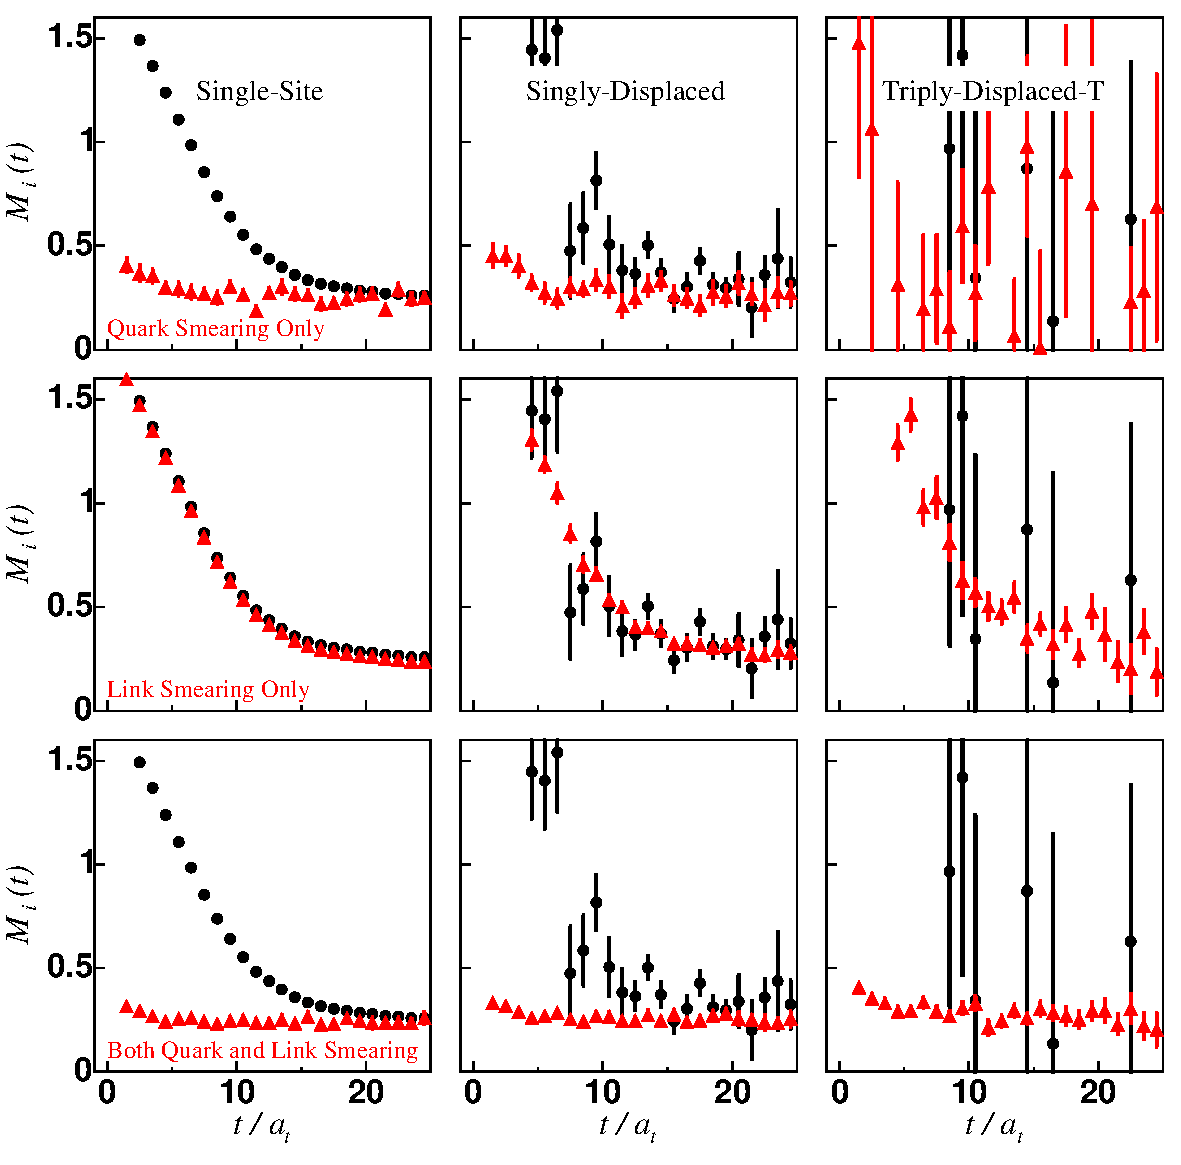
\includegraphics[scale=0.8]{figures/meff-smearing.pdf}
        \caption{Insert caption, cite spectroscopy.}\label{fig:meff-smearing}
    \end{figure}
    
    $\tilde\Delta$ is Hermitian, and we define its eigenvalues as $-\lambda^{(k)}$ (ordered by increasing $\lambda^{(k)}$) and their corresponding orthonormal eigenvectors as $v^{(k)}$. Then, if we define the smearing kernel in Eq.~\ref{eq:quark_smearing} as $K=\left(1+\frac{\sigma_{s}^{2}}{4 n_{\sigma}} \widetilde{\Delta}\right)^{n_{\sigma}}$, we can express the kernel in the eigenbasis of the GCL:
    \begin{equation}
        K_{a b}(x, y)=\delta_{x_{4}, y_{4}} \sum_{k} w_{k}\,v_{a}^{(k)}(x) v_{b}^{(k)}(y)^{*},
    \end{equation}
    where we suppress the flavor index, and where $w_k\in\mathbb{R}^+$. Since $K$ is written in terms of $\tilde\Delta$, it is trivial to write down,
    \begin{equation}
        w_{k}=\left(1-\frac{\sigma_{s}^{2}}{4 n_{\sigma}} \lambda^{(k)}\right)^{n_{\sigma}}.
    \end{equation}
    It is then also easy to see that,
    \begin{equation}
        \lim _{n_{\sigma} \rightarrow \infty} w_{k}=\exp \left(-\frac{1}{4} \sigma_{s}^{2} \lambda^{(k)}\right).
    \end{equation}
    We can now see the advantage of working in the eigenbasis of the GCL: the weights, $w_{k}$, of higher modes of $\tilde\Delta$ are exponentially suppressed. We can then investigate the possibility of modifying the weights to neglect higher-lying contributions. One simple way to accomplish this is the so-called \emph{Laplacian Heaviside} (LapH) smearing scheme, introduced by Peardon, Morningstar, et al. in ~\cite{PhysRevD.80.054506}. This procedure sets the weights to be,
    \begin{equation}
        w_{k}=\Theta\left(\sigma_{s}^{2}-\lambda^{(k)}\right),
    \end{equation}
    where $\Theta$ is the Heaviside step function, and $\sigma_s^2$ acts as a hard cutoff. The LapH smearing kernel is now defined as
    \begin{equation}
        \mathcal{S}=\Theta\left(\sigma_{s}^{2}+\widetilde{\Delta}\right),
    \end{equation}
    and our smeared quark fields are now given by
    \begin{equation}
        \widetilde\psi(x) = \mathcal{S}\psi(x).
    \end{equation}

    \subsection{Displacements}
    The motivation for displacing the quark fields is hadrons are objects which are extended in space. Therefore, if we hope to capture radial and orbital structure when computing the hadronic correlation functions, then we must displace the quark fields, and do so in a gauge-covariant way. The displacements we consider are straight-path displacements along the spatial lattice unit vectors: $j = \pm 1, \pm 2, \pm 3$. We define the gauge-covariant displacement operator in the $j^{\mathrm{th}}$ direction by,
    \begin{equation}
        \widetilde{D}_{j}^{(p)}\left(x, x^{\prime}\right)=\widetilde{U}_{j}(x) \widetilde{U}_{j}(x+\hat{j}) \ldots \widetilde{U}_{j}(x+(p-1) \hat{j}) \delta_{x^{\prime}, x+p \hat{j}},
    \end{equation}
    where $p \geq 1$ denotes the number of steps in by which the field is displaced. For convenience, we also define a zero-displacement operator, $\widetilde{D}_{0}^{(p)}\left(x, x^{\prime}\right)=\delta_{x x^{\prime}}.$ Including color indices $a$ and $a^\prime$, it can be shown that $\widetilde{D}_{j}^{(p) \dagger}\left(x, x^{\prime}\right)^{a a^{\prime}}=\widetilde{D}_{-j}^{(p)}\left(x, x^{\prime}\right)^{a a^{\prime}}.$ From this, the following useful properties can be derived:
    \begin{equation}
        \begin{aligned}
            \left(\widetilde{D}_{j}^{(p)} \psi\right)(x)&=\sum_{x^{\prime}} \widetilde{D}_{j}^{(p)}\left(x, x^{\prime}\right) \psi\left(x^{\prime}\right)=\widetilde{U}_{j}(x) \widetilde{U}_{j}(x+\hat{j}) \ldots \widetilde{U}_{j}(x+(p-1) \hat{j}) \psi(x+p \hat{j}),\\
            \left(\overline{\chi} \widetilde{D}_{j}^{(p) \dagger}\right)(x)&=\sum_{x^{\prime}} \overline{\chi}\left(x^{\prime}\right) \widetilde{D}_{j}^{(p) \dagger}\left(x^{\prime}, x\right)=\sum_{x^{\prime}} \overline{\chi}\left(x^{\prime}\right) \widetilde{D}_{-j}^{(p)}\left(x^{\prime}, x\right)\\
            &=\overline{\chi}(x+p \hat{j}) \widetilde{U}_{j}^{\dagger}(x+(p-1) \hat{j}) \ldots \widetilde{U}_{j}^{\dagger}(x+\hat{j}) \widetilde{U}_{j}^{\dagger}(x),
        \end{aligned}
    \end{equation}
    from which it can be seen,
    \begin{equation}
        \overline{\chi}(x)\left(\widetilde{D}_{j}^{(p)} \psi\right)(x)=\left(\overline{\chi} \widetilde{D}_{j}^{(p)}\right)(x) \psi(x).
    \end{equation}
    {\color{red}Why do we have to show associativity? Why would it not be obvious?}

    The final building blocks for our hadronic operators are \emph{covariantly-displaced, smeared quark fields} and can be summarized as follows:
    \begin{equation}
        \boxed{\left(\widetilde{D}_{j_{1}}^{(p)} \ldots \widetilde{D}_{j_{n}}^{(p)} \widetilde{\psi}\right)_{a \alpha}^{A}, \quad\left(\widetilde{\chi} \widetilde{D}_{j_{1}}^{(p) \dagger} \ldots \widetilde{D}_{j_{n}}^{(p) \dagger}\right)_{a \alpha}^{A}, \quad-3 \leq j_{i} \leq 3.}
    \end{equation}
    {\color{red}Add in graphics showing types of displacements we use.}

    \section{Symmetries on the Lattice}
    Symmetries are very useful for characterizing and labeling stationary states in quantum mechanics. Conserved quantities, such as momentum and charge, emerge from the symmetries of a given system, and so in order to identify the relevant quantum numbers of a theory, we must identify its relevant symmetries. The primary symmetries we are interested in are: (cubic) rotations, $G$-parity, isospin, and flavor. SU(3) gauge symmetry is also vital, but since all of the final objects we study are colorless, it does not contribute to how we label stationary states.
    
    \subsection{Rotations}
    Given the nature of a discrete, finite-volume lattice, one can easily see that the SO(3) rotation group is no longer a symmetry group of any lattice gauge theory. Because of this, angular momentum is not conserved on the lattice, and therefore angular momentum is no longer a good quantum number. We will see that instead of using the irreducible representations (irreps) of SO(3) to label stationary states, we use the irreps of the octahedral group.

    To aid in discussions of cubic rotations on the lattice, the following notation will be used, where the axes of rotation, $j = x,y,z,a,b,c,d,\alpha,\beta,\gamma,\delta$, are shown in Fig.~\ref{fig:rotation_axes}:
    \begin{equation}
        \begin{aligned}
            E &: \text{the identity}\\
            C_{nj} &: \text{proper rotation of angle}\ \frac{2\pi}{n}\ \text{about the axis}\ O_j\text{, where}\ n = 2,3,4 \\
            I_s &: \text{spatial inversion}
        \end{aligned}
    \end{equation}
    \begin{figure}
        \centering
        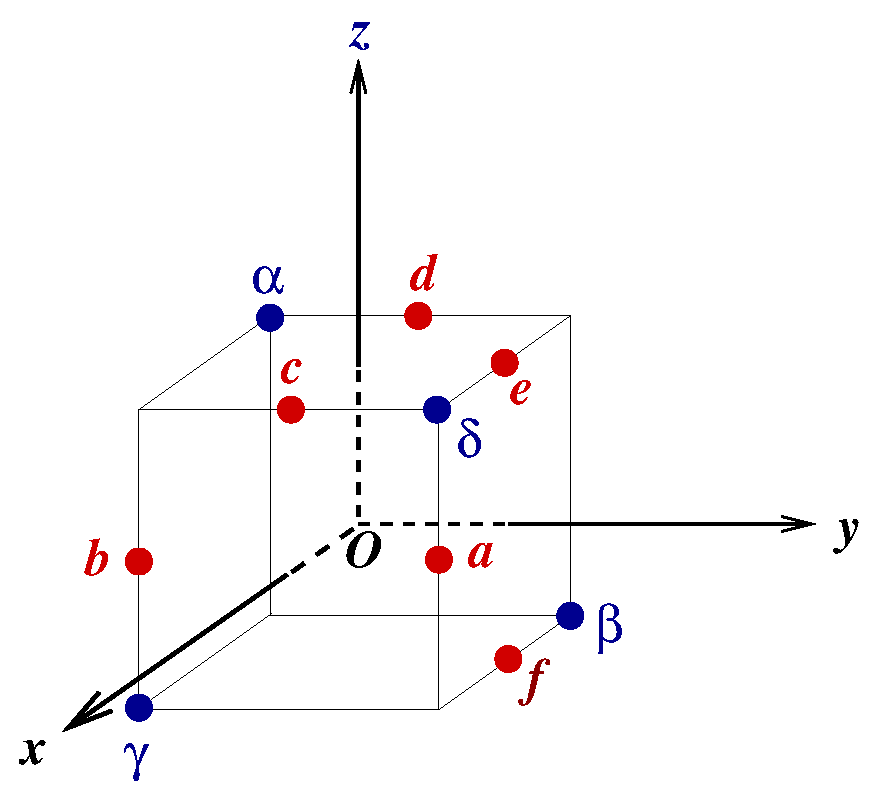
\includegraphics[scale=0.5]{figures/Oaxes.pdf}
        \caption{The rotation axes corresponding to the rotations $C_{nj}$. Figure taken from Ref.~\cite{}}
        \label{fig:rotation_axes}
    \end{figure}
    The octahedral point group, $O$, consists of all allowed rotations on a three-dimensional spatially-isotropic cubic lattice, and contains the following elements:
    \begin{table}[h!]
        \centering
        \begin{tabular}{l|l}
            Group element & Axes, $j$\\
            \hline
            $E$ & \\
            $C_{4j}$, $C_{4j}^{-1}$ & $x,y,z$ \\
            $C_{2j}$ & $x,y,z,a,b,c,d,e,f$ \\
            $C_{3j}$, $C_{3j}^{-1}$ & $\alpha,\beta,\gamma,\delta$
        \end{tabular}
        \label{table:O}
    \end{table}

    There are five irreps of $O$. Following the Mulliken convention~\cite{}, they are named $A_1$, $A_2$, $E$, $T_1$, $T_2$, and they have dimensions 1, 1, 2, 3, 3, respectively. In order to make connections to infinite-volume continuum physics, the Table~\ref{table:O_occurrence_nums} gives the \emph{occurrence numbers} $n_\Gamma^J$, which are the number of times the irrep $\Gamma$ of $O$ occurs in the subduction of the irrep $J$ of SO(3).

    When we take the direct product of $O$ with the group $\lbrace E,I_s \rbrace$, thereby adding in spatial inversions to our proper rotations, we get what is known as the point group $O_h$. This group has twice the number of irreps as $O$, and so we add the labels $g/u$ (standing for the German \emph{gerade} and \emph{ungerade}) to our irreps, which denote even and odd parity, respectively. The irreps of $O_h$ are $A_{1g}$, $A_{1u}$, $A_{2g}$, $A_{2u}$, $E_g$, $E_u$, $T_{1g}$, $T_{1u}$, $T_{2g}$, and $T_{2u}$.

    When we incorporate spin into the picture, we must introduce a new generator that represents rotating by $2\pi$ about any axis. Doing so, we arrive at the double octahedral point group $O^D$. Sparing the group-theoretical details, $O^D$ has three irreps in addition to all of the irreps of $O$. These are named $G_1$, $G_2$, and $H$, and are of dimension 2, 2, and 4, respectively. Table~\ref{table:OD_occurrence_nums} gives the occurrence numbers of these three additional numbers in the subductions of the $J$ irreps of SU(2). Like for $O_h$, when we incorporate spatial inversions into $O^D$, we arrive at the double point group $O_h^D$, which has twice the number of irreps of $O^D$. The additional irreps are $G_{1g}$, $G_{1u}$, $G_{2g}$, $G_{2u}$, $H_g$, and $H_u$.

    \renewcommand{\arraystretch}{1.2}
    \begin{table}
        \centering
        \begin{minipage}{.4\linewidth}
        \centering
        \begin{tabular}{l|l|l|l|l|l}
            $J$ & $n_{A_1}^J$ & $n_{A_2}^J$ & $n_{E}^J$ & $n_{T_1}^J$ & $n_{T_2}^J$\\
            \hline
            0 & 1 & 0 & 0 & 0 & 0\\
            1&0&0&0&1&0\\
            2&0&0&1&0&1\\
            3&0&1&0&1&1\\
            4&1&0&1&1&1\\
            \vdots & \vdots & \vdots & \vdots & \vdots & \vdots
        \end{tabular}
        \caption{}
        \label{table:O_occurrence_nums}
        \end{minipage}
        \begin{minipage}{.4\linewidth}
        \centering
        \begin{tabular}{l|l|l|l}
            $J$ & $n_{G_1}^J$ & $n_{G_2}^J$ & $n_{H}^J$ \\
            \hline
            $\frac{1}{2}$&1&0&0\\
            $\frac{3}{2}$&0&0&1\\
            $\frac{5}{2}$&0&1&1\\
            $\frac{7}{2}$&1&1&1\\
            $\frac{9}{2}$&1&0&2\\
            \vdots&\vdots&\vdots&\vdots
        \end{tabular}
        \caption{}
        \label{table:OD_occurrence_nums}
        \end{minipage}
    \end{table}
    \renewcommand{\arraystretch}{1.0}
    \subsubsection{Moving irreps}
    In order to construct operators that create and annihilate particles of definite momentum $\boldsymbol p$, we must subduce the representations of $O_h^D$ onto the little group of $\boldsymbol p$. The little group of $\boldsymbol p$ consists of the subgroup of the abelian group of lattice translations which leave the momentum invariant. For $\boldsymbol p = (0, 0, 0)$, the little group is simply the point group $O_h$. For any on-axis momentum, e.g. $\boldsymbol p = (0, 0, 1)$, the little group is $C_{4v}$, which includes four rotations of angle $\frac{\pi}{2}$ about the axis along $\boldsymbol p$, as well as four reflections about reflection planes containing that axis. The group elements are contained in three conjugacy classes, which are included in Table~\ref{table:c4vD}.  For any planar-diagonal momentum, e.g. $\boldsymbol p = (0, 1, 1)$, the little group is $C_{2v}$, the elements and conjugacy classes of which are included in Table~\ref{table:c2vD}. For any cubic-diagonal fmomentum, e.g. $\boldsymbol p = (1,1,1)$, the little group is $C_{3v}$; its elements and their conjugacy classes are includeds in Table~\ref{table:c3vD}. Additionally, in order to construct the analogous spinorial little groups (called $C_{4v}^D$, $C_{2v}^D$, and $C_{3v}^D$, respectively), we include the $2\pi$-rotation generator $\overline E$. Tables~\ref{table:c4vD}---\ref{table:c3vD} give the elements and conjugacy classes for the spinorial little groups.
    \begin{table}
        \centering
        \begin{minipage}{0.32\linewidth}
            \begin{tabular}{l|l}
                $C_{4vD}$ & \\
                \hline
                $\mathcal{C}_{1}$ & $\{E\}$ \\
                $\mathcal{C}_{2}$ & $\left\{C_{2 z}, \overline{C}_{2 z}\right\}$ \\
                $\mathcal{C}_{3}$ & $\left\{C_{4 z}, C_{4 z}^{-1}\right\}$ \\
                $\mathcal{C}_{4}$ & $\left\{I_{s} C_{2 x}, I_{s} C_{2 y},\right.$\\
                & $\left.\quad I_{s} \overline{C}_{2 x}, I_{s} \overline{C}_{2 y}\right\}$ \\
                $\mathcal{C}_{5}$ & $\left\{I_{s} C_{2 a}, I_{s} C_{2 b},\right.$\\
                & $\left.\quad I_{s} \overline{C}_{2 a}, I_{s} \overline{C}_{2 b}\right\}$ \\
                $\mathcal{C}_{6}$ & $\{\overline{E}\}$ \\
                $\mathcal{C}_{7}$ & $\left\{\overline{C}_{4 z}, \overline{C}_{4 z}^{-1}\right\}$
            \end{tabular}
            \caption{}
            \label{table:c4vD}
        \end{minipage}
        \begin{minipage}{0.32\linewidth}
            \begin{tabular}{l|l}
                $C_{2vD}$ & \\
                \hline
                $\mathcal{C}_{1}$ & $\{E\}$ \\
                $\mathcal{C}_{2}$ & $\left\{C_{2 e}, \overline{C}_{2 e}\right\}$ \\
                $\mathcal{C}_{3}$ & $\left\{I_{s} C_{2 f}, I_{s} \overline{C}_{2 f}\right\}$ \\
                $\mathcal{C}_{4}$ & $\left\{I_{\overline{c}} C_{2 f}, I_{s} \overline{C}_{2 x}\right\}$ \\
                $\mathcal{C}_{5}$ & $\{\overline{E}\}$
            \end{tabular}
            \caption{}
            \label{table:c2vD}
        \end{minipage}
        \begin{minipage}{0.32\linewidth}
            \begin{tabular}{l|l}
                $C_{3vD}$ & \\
                \hline
                $\mathcal{C}_{1}$ & $\{E\}$ \\
                $\mathcal{C}_{2}$ & $\left\{C_{3 \delta}, C_{3 \delta}^{-1}\right\}$ \\
                $\mathcal{C}_{3}$ & $\left\{I_{s} C_{2 b}, I_{s} C_{2 d}, I_{s} C_{2 f}\right\}$ \\
                $\mathcal{C}_{4}$ & $\{\overline{E}\}$ \\
                $\mathcal{C}_{5}$ & $\left\{\overline{C}_{3 \delta}, \overline{C}_{3 \delta}^{-1}\right\}$ \\
                $\mathcal{C}_{6}$ & $\left\{I_{s} \overline{C}_{2 b}, I_{s} \overline{C}_{2 d}, I_{s} \overline{C}_{2 f}\right\}$
            \end{tabular}
            \caption{}
            \label{table:c3vD}
        \end{minipage}
    \end{table}               
    Finally, the subductions of the irreps of $O_h^D$ onto the above little groups leaves us with the irreps in which we expect to find moving particles. These subductions are given in Table~\ref{table:subductions}.
    \begin{table}
        \centering
        \begin{tabular}{c|c|c|c}
            $\Lambda(O_h)$ & $\Lambda(O_h)\downarrow C_{4v}$ & $\Lambda(O_h) \downarrow C_
            {3v}$ & $\Lambda(O_h) \downarrow C_{2v}$ \\
            \hline
            $A_{1g}$ & $A_1$ & $A_1$ & $A_1$ \\
            $A_{1u}$ & $A_2$ & $A_2$ & $A_2$ \\
            $A_{2g}$ & $B_1$ & $A_2$ & $B_2$ \\
            $A_{2u}$ & $B_2$ & $A_1$ & $B_1$ \\
            $E_g$ & $A_1 \oplus B_1$ & $E$ & $A_1 \oplus B_2$ \\
            $E_u$ & $A_2 \oplus B_2$ & $E$ & $A_2 \oplus B_1$ \\
            $T_{1g}$ & $A_2 \oplus E$ & $A_2 \oplus E$ & $A_2 \oplus B_1 \oplus B_2$ \\
            $T_{1u}$ & $A_1 \oplus E$ & $A_1 \oplus E$ & $A_1 \oplus B_1 \oplus B_2$ \\
            $T_{2g}$ & $B_2 \oplus E$ & $A_1 \oplus E$ & $A_1 \oplus A_2 \oplus B_1$ \\
            $T_{2u}$ & $B_1 \oplus E$ & $A_2 \oplus E$ & $A_1 \oplus A_2 \oplus B_2$ \\
            $G_{1g/u}$ & $G_1$ & $G$ & $G$ \\
            $G_{2g/u}$ & $G_2$ & $G$ & $G$ \\
            $H_{g/u}$ & $G_1 \oplus G_2$ & $F_1 \oplus F_2 \oplus G$ & $2G$
        \end{tabular}
        \caption{}
        \label{table:subductions}
    \end{table}

    \subsection{Isospin and Quark Flavor}
    The physical mass of the up quark is $m_u = 2.16^{+0.49}_{-0.26}$ MeV and the physical mass of the down quark is $m_d = 4.67^{+0.48}_{-0.17}$ MeV~\cite{PhysRevD.98.030001}. While these masses differ by more than a factor of 2, their difference is very small compared to the next heaviest quark, which is the strange quark, measuring at $m_s = 93^{+11}_{-5}$ MeV~\cite{PhysRevD.98.030001}. Therefore, we find it justfied to make an approximation and set $m_u = m_d$ in our calculations. Since QCD conserves flavor (we do not include electroweak interactions), our theory now possesses an internal SU(2) symmetry, the conserved quantity of which is referred to as \emph{isospin}. This has the same mathematical structure as normal spin, and we can therefore think of it analogously, but it should be stressed that isospin has no relation to physical space and does not denote any kind of angular momentum. The up quark and down quark states can then be thought of as a doublet of states having total isospin $I=\frac{1}{2}$. Just like with SU(2) spin, isospin can be decomposed onto three axes. By convention, we assign the third isospin axis component of the up quark to be $I_3 = \frac{1}{2}$ and of the down quark to be $I_3 = -\frac{1}{2}$. Their corresponding antiparticles have the same $I$, but $I_3\rightarrow -I_3$. The work presented here is done in a theory of $N_f = 2 + 1$ QCD, meaning our theory contains two \emph{light} quarks, referring to the up and down quarks (the strange quark is sometimes referred to as a light quark in other contexts), and a strange quark.
    
    Under an SU(2) isospin rotation of the form
    \begin{equation}
        U_{R_{\tau}}=\exp{-i\alpha\tau_3}\exp{-i\beta\tau_2}\exp{-i\gamma\tau_3} = \exp (-i \boldsymbol{\varphi} \cdot \boldsymbol{\tau}),
    \end{equation}
    where $\tau_1$, $\tau_2$, $\tau_3$ are the three generators of isospin rotations,
    an operator $\overline O_{I_3}^{(I)}$ transforms according to the $I$ irreducible representation as
    \begin{equation}
        U_{R_{\tau}}\overline O_{I_3}^{(I)}U_{R_{\tau}}^\dagger = \sum_{I_3^\prime} \overline O_{I_3^\prime}^{(I)} D^{(I)}_{I_3^\prime, I_3}(R_\tau),
    \end{equation}
    where $D^{(I)}(R_\tau)$ are the Wigner rotation matrices. In order for an operator $\overline O_{I_3}^{(I)}$ to transform irreducibly under isospin, it must satisfy the following properties:
    \begin{align}
        \left[\tau_3, \overline O_{I_3}^{(I)}\right] &= I_3 \overline O_{I_3}^{(I)}, \\
        \left[\tau_+, \overline O_{I_3}^{(I)}\right] &= \sqrt{(I - I_3)(I + I_3 + 1)} \overline O_{I_3 + 1}^{(I)}, \\
        \left[\tau_-, \overline O_{I_3}^{(I)}\right] &= \sqrt{(I + I_3)(I - I_3 + 1)} \overline O_{I_3 - 1}^{(I)}, \\
        \left[\tau_3, \left[\tau_3, \overline O_{I_3}^{(I)}\right] \right] + \frac{1}{2} \left[\tau_+, \left[\tau_-, \overline O_{I_3}^{(I)}\right]\right] &+ \frac{1}{2}\left[\tau_-, \left[\tau_+, \overline O_{I_3}^{(I)}\right]\right] = I(I + 1) \overline O_{I_3}^{(I)},
    \end{align}
    where $\tau_\pm = \tau_1 \pm i\tau_2$. For annihilation operators, an operator $O_{I_3}^{(I)}$ should transform according to the $I$ irreducible representation as
    \begin{equation}
        U_{R_{\tau}}O_{I_3}^{(I)}U_{R_{\tau}}^\dagger = \sum_{I_3^\prime} O_{I_3^\prime}^{(I)} D^{(I)}_{I_3^\prime, I_3}(R_\tau)^*.
    \end{equation}
    Annihilation operators that are irreducible under isospin rotations should satisfy:
    \begin{align}
        \left[\tau_3, O_{I_3}^{(I)}\right] &= -I_3 O_{I_3}^{(I)}, \\
        \left[\tau_+, O_{I_3}^{(I)}\right] &= -\sqrt{(I - I_3)(I + I_3 + 1)} O_{I_3 + 1}^{(I)}, \\
        \left[\tau_-, O_{I_3}^{(I)}\right] &= -\sqrt{(I + I_3)(I - I_3 + 1)} O_{I_3 - 1}^{(I)}, \\
        \left[\tau_3, \left[\tau_3, O_{I_3}^{(I)}\right] \right] + \frac{1}{2} \left[\tau_+, \left[\tau_-, O_{I_3}^{(I)}\right]\right] &+ \frac{1}{2}\left[\tau_-, \left[\tau_+, O_{I_3}^{(I)}\right]\right] = I(I + 1)  O_{I_3}^{(I)}.
    \end{align}
    \subsection{Charge Conjugation and $G$-Parity}
    $C$-parity can only be a symmetry for electrically neutral states, but as pure QCD does not see electric charge, we are motivated to generalize $C$-parity in order to account states in a charged isospin multiplet, such as the pion triplet. With $\mathcal C$ denoting the charge conjugation operator, $G$-parity can be explicitly defined as
    \begin{equation}
        U_G = \mathcal C e^{-i\pi\tau_2}.
    \end{equation}
    Since charge conjugation is a symmetry of the strong interaction, then when isospin is also a symmetry, $G$-parity must be a symmetry as well. The basic building blocks transform under $G$-parity as follows~\cite{ref:spectroscopy}:
    \begin{align} U_{G}\left(D_{j} \mathcal S \psi(x)\right)_{a \alpha}^{u} U_{G}^{\dagger} &=-\left(\chi \mathcal S D_{j}^{\dagger}(x)\right)_{a \beta}^{d} \Gamma_{\beta \alpha}^{G}, \\ U_{G}\left(D_{j}\mathcal S \psi(x)\right)_{a \alpha}^{d} U_{G}^{\dagger} &=\left(\chi \mathcal S D_{j}^{\dagger}(x)\right)_{a \beta}^{u} \Gamma_{\beta \alpha}^{G}, \\ U_{G}\left(D_{j} \mathcal S \psi(x)\right)_{a \alpha}^{s} U_{G}^{\dagger} &=-\left(\chi \mathcal S D_{j}^{\dagger}(x)\right)_{a \beta}^{s} \Gamma_{\beta \alpha}^{G}, \\ U_{G}\left(\chi \mathcal S D_{j}^{\dagger}(x)\right)_{a \alpha}^{u} U_{G}^{\dagger} &=-\Gamma_{\alpha \beta}^{C}\left(D_{j} \mathcal S \psi(x)\right)_{a \beta}^{u}, \\ U_{G}\left(\chi \mathcal S D_{j}^{\dagger}(x)\right)_{a \alpha}^{a} U_{G}^{\dagger} &=\Gamma_{\alpha \beta}^{G}\left(D_{j} \mathcal S \psi(x)\right)_{a \beta^{\prime}}^{u}, \\ U_{G}\left(\chi \mathcal S D_{j}^{\dagger}(x)\right)_{a \alpha}^{s} U_{G}^{\dagger} &=-\Gamma_{\alpha \beta}^{C}\left(D_{j} \mathcal S \psi(x)\right)_{a \beta}^{s}. \end{align}
    \subsection{Projecting Operators onto Symmetry Sectors}

    \section{Single-Hadron Operator Construction}
    \subsection{Baryon Operators}
    Baryon states are classified according to: momentum $\boldsymbol p$, total spin $J$, spin projection $J_z$ (or any other axis), parity $P$ ($\pm 1)$, and quark flavor. The flavor quantum numbers we consider are isospin $I$ and its projection $I_3$, and strangeness $S$. We require that baryon operators are also gauge-invariant. As a reminder, the basic building blocks for the baryon operators are covariantly-displaced smeared quark fields.
    \subsubsection{Elemental Baryons}
    An \emph{elemental} operator is simply one that is created with proper color structure, definite flavor structure, definite position or momentum, but has not been projected onto relevant symmetry sectors.
    \subsection{Meson Operators}
    \subsection{Tetraquark Operators}
    \section{Multi-Hadron Operator Construction}

\chapter{Calculation of Correlators using the Stochastic LapH Method}\label{ch:montecarlo}
In Ch.~\ref{ch:latticeqcd}, we saw that calculating two-point correlation functions on the lattice using the Monte Carlo method involves evaluating some function of the inverse of the Dirac matrix, i.e.\ some function of the quark propagator. The task of inverting the Dirac matrix is a formidable one. The Dirac matrix carries indices for spacetime, color, and Dirac spin, so for a theory of three colors and four Dirac indices on a $32^3\times 256$ lattice, this amounts to a complex-valued matrix of size $\sim 10^8\times 10^8$. Storing such a matrix in single precision would take roughly 80 petabytes, and so calculating the inverse directly is obvious unfeasible. In this chapter we will discuss methods to tackle this problem that involve stochastically estimating Dirac matrix inverses. We will see that the path integration over the quark fields can be done analytically, but it results in a complicated expression involving the gluon field. The path integration over the gluon field must be estimated using Monte Carlo methods.
\section{Quark Lines}
Calculating a correlator on the lattice involves integrating first over quark fields which are complex Grassmann valued. Recall from Ch.~\ref{ch:latticeqcd} that such an integration results in some function $f$ of the Dirac matrix inverse and the determinant of the Dirac matrix. For example, a meson correlator involves an integral of the form
\begin{equation}
    \int \mathcal{D}[\overline{\psi}, \psi] \psi_{a} \psi_{b} \overline{\psi}_{c} \overline{\psi}_{d} \exp \left(-\overline{\psi}^{T} M \psi\right) = \left(M_{a d}^{-1} M_{b c}^{-1}-M_{a c}^{-1} M_{b d}^{-1}\right) \det M,
\end{equation}
and a baryonic correlator inolves an integral of the form
\begin{eqnarray}
    &&\int {\cal D}[\overline{\psi},\psi]\ \psi_{a_1}\psi_{a_2}\psi_{a_3}
       \ \overline{\psi}_{b_1}\overline{\psi}_{b_2}\overline{\psi}_{b_3}
     \ \exp\left( -\overline{\psi}^T M \psi \right)\nonumber\\
     &=&\biggl( - M_{a_1b_1}^{-1}M^{-1}_{a_2b_2}M^{-1}_{a_3b_3}
     +M^{-1}_{a_1b_1}M^{-1}_{a_2b_3}M^{-1}_{a_3b_2}
      +M^{-1}_{a_1b_2}M^{-1}_{a_2b_1}M^{-1}_{a_3b_3} \nonumber\\
    && \phantom{\biggl(}-M_{a_1b_2}^{-1}M^{-1}_{a_2b_3}M^{-1}_{a_3b_1}
     -M^{-1}_{a_1b_3}M^{-1}_{a_2b_1}M^{-1}_{a_3b_2}
      +M^{-1}_{a_1b_3}M^{-1}_{a_2b_2}M^{-1}_{a_3b_1}   
      \biggr)\ \det M.
      \label{eq:barywick}
\end{eqnarray}
In general, including the fact that our quark fields are smeared and covariantly displaced, so the Grassmann integrals we need to compute are really of the form
\begin{equation}
    \int \mathcal{D}[\chi, \psi] \sum_{\alpha d} f_{a c} \psi_{c} \chi_{d} g_{d b} \exp \left(-\chi^{T} \Omega \psi\right)=\sum_{c d} f_{a c} \Omega_{c d}^{-1} g_{d b} \operatorname{det} \Omega,
\end{equation}
where we have made the substitutions $\chi \equiv \overline \psi \gamma_4$ and $\Omega = \gamma_4 M$, and where $f_{ac}$ and $g_{db}$ are $c$-number coefficients. Each factor of $\Omega^{-1}$ is referred to as a \emph{quark line}. When computing temporal correlators, we can classify quark lines as follows:
\begin{itemize}
    \item forward-time quark lines originate from $\chi$ at a time $t_0$ and terminate to $\psi$ at a later time $t$
    \item backward-time quark lines originate from $\chi$ at a time $t$ and terminate to $\psi$ at an earlier time $t_0$
    \item same-time quark lines originate from $\chi$ and terminate to $\psi$ at the same time, either $t$ or $t_0$.
\end{itemize}
In a two-point correlator, $t_0$ is referred to as the \emph{source time} and $t$ is referred to as the \emph{sink time}. These different types of quark lines are depicted in Fig.~\ref{fig:quark_lines}. Recall the definition of the smearing operator $\mathcal S$ from Eq.~(\ref{eq:smearing_operator}) and the covariant displacement operator $D$ from Eq.~(\ref{eq:displacement_operator}). The quark lines we work with in practice arise from smeared and displaced quark and antiquark fields, so we refer to
\begin{equation}
    (D_{j})_{a b} \mathcal{S}_{b c} \Omega_{c h}^{-1} \mathcal{S}_{h g}(D_{k}^{\dagger})_{g f}=(D_{j} \mathcal{S} \Omega^{-1} \mathcal{S} D_{k}^{\dagger})_{a f}
\end{equation}
as a forward-time quark line and for convenience denote this by,
\begin{equation}
    Q_{j k}\left(t, t_{0}\right)=D_{j} \mathcal{S} \Omega^{-1}\left(t, t_{0}\right) \mathcal{S} D_{k}^{\dagger}.
\end{equation}
Similarly, a backward-time quark line is given by~\cite{spectroscopy},
\begin{equation}
    \overline{Q}_{j k}\left(t, t_{0}\right)=\left(\gamma_{5} \gamma_{4} Q_{j k}\left(t, t_{0}\right) \gamma_{4} \gamma_{5}\right)^{*} = -Q_{kj}(t_0,t),
\end{equation}
and a same-time quark line is given by $Q_{jk}(t,t)$. 
\begin{figure}
    \centering
    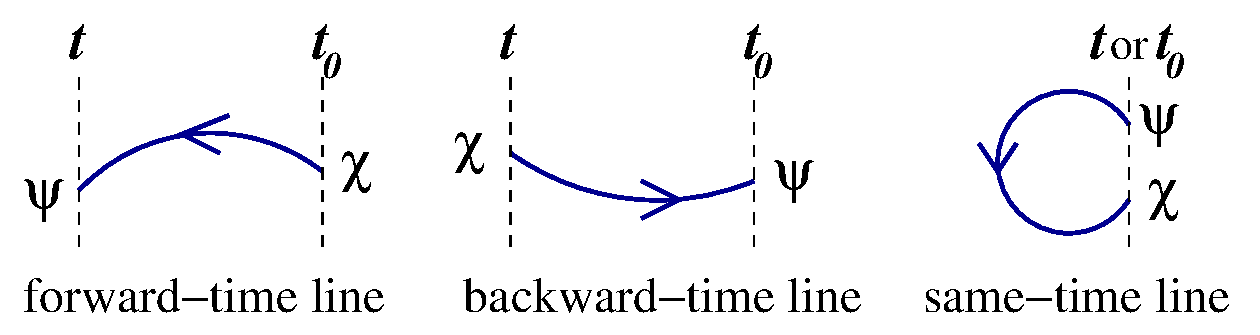
\includegraphics[width=6in]{figures/quarklines.pdf}
    \caption[The three types of quark lines that occur by integrating the quark fields when evaluating two-point temporal correlators.]{The three types of quark lines that occur by integrating the quark fields when evaluating two-point temporal correlators. Figure taken from Ref.~\cite{spectroscopy}.}
    \label{fig:quark_lines}
\end{figure}
\section{Motivating the Need for Stochastically Estimated All-to-All Propagators}
A single-hadron operator of definite momentum (consider $\bs p = 0$ without loss of generality) is a Fourier transform involving a summation over all spatial sites:
\begin{equation}
    \mathcal{O}(\boldsymbol{p}= 0, t)=\frac{1}{V} \sum_{\boldsymbol{x}} \varphi(\boldsymbol{x}, t),
\end{equation}
where $\varphi(\bs x, t)$ is a single-hadron operator located at a spatial site $\bs x$ at time $t$ and $V$ is the spatial volume of the lattice. A two-point correlator for such a hadron has the form
\begin{equation}
    C(t) = \frac{1}{V^2} \sum_{\bs x, \bs y} \bra 0\varphi(\bs x, t+t_0)\overline\varphi(\bs y, t_0) \ket 0.
\end{equation}
Calculating such a correlator appears to involve evaluating quark propagators from all spatial sites $\bs x$ to all spatial sites $\bs y$, which is an expensive computation. These are known as \emph{all-to-all} propagators. A trick can be used to avoid this by exploiting translational invariance to remove one of the spatial sums, giving
\begin{equation}
    C(t) = \frac{1}{V} \sum_{\bs x} \bra 0 \varphi(\bs x, t+t_0) \overline\varphi(0, t_0) \ket 0.
\end{equation}
Now we are tasked with evaluating the quark propagator from one single site (the origin) to all spatial site, which is a much easier task. These propagators are known as \emph{point-to-all} propagators.

Unfortunately, we cannot use this translational invariance trick in all cases. Many of our calculations necessitate the use of multi-hadron correlators (for example, if we wish to study resonances). If we consider a two-hadron operator with zero total momentum and back-to-back constituent momentum, such an operator has the form
\begin{equation}
    \mathcal{O}_{1}(\boldsymbol{p}, t) \mathcal{O}_{2}(-\boldsymbol{p}, t)=\frac{1}{V^{2}} \sum_{\boldsymbol{x}, \boldsymbol{y}} \varphi_{1}(\boldsymbol{x}, t) \varphi_{2}(\boldsymbol{y}, t) e^{-i \boldsymbol{p}(\boldsymbol{x}-\boldsymbol{y})}.
\end{equation}
When forming a two-point correlator with such an operator, we can no longer exploit translational variance to remove the need of calculating all-to-all propagators.

Additionally, calculations involving disconnected diagrams (such isoscalar meson correlators) are not amenable to point-to-all methods. Many calculations in the past have neglected contributions from disconnected diagrams, but such calculations ignore important sea quark effects which have a demonstrable effect on the resulting spectrum. There is therefore a need for a method that can efficiently calculate all-to-all propagators.
\section{Stochastically Estimating the Quark Propagator}
Since calculating Dirac matrix inverses is just an intermediate step in a larger Monte Carlo calculation, the accuracy of which is determined by the uncertainty in sampling over the gauge fields, it is unnecessary to calculate these inverses exactly. We can instead use Monte Carlo subsampling, or Monte Carlo within Monte Carlo, to stochastically estimate the quark propagators on each gauge configuration. Consider an $N\times N$ complex matrix $M$ whose inverse we wish to stochastically estimate, and a random noise vector $\eta$ whose expectations satisfy $E(\eta_i) = 0$ and $E(\eta_i \eta_j^*) = \delta_{ij}$. Assume that for any $\eta$ we can solve (say, by some variation of the conjugate gradient method) $MX=\eta$ for $X$. Then $X=M^{-1}\eta$ and
\begin{equation}
    E\left(X_{i} \eta_{j}^{*}\right)=E\left(\sum_{k} M_{i k}^{-1} \eta_{k} \eta_{j}^{*}\right)=\sum_{k} M_{i k}^{-1} E\left(\eta_{k} \eta_{j}^{*}\right)=\sum_{k} M_{i k}^{-1} \delta_{k j}=M_{i j}^{-1}.
\end{equation}
We can then in principle obtain a Monte Carlo estimate of $M^{-1}_{ij}$ by sampling over $N_R$ random noise vectors:
\begin{equation}
    M_{i j}^{-1} \approx \lim _{N_{R} \rightarrow \infty} \frac{1}{N_{R}} \sum_{r=1}^{N_{R}} X_{i}^{(r)} \eta_{j}^{(r) *}, \quad \text { where } M X^{(r)}=\eta^{(r)}.
\end{equation}
In practice, the variances that result in estimating Dirac matrix inverses in this way are too large to be useful. Notice that the above estimate only becomes exact in the limit of $N_R\rightarrow \infty$ which requires the computation of an infinite amount of solution vectors, whereas we can achieve an exact result by only solving $N$ linear systems. A technique known as \emph{dilution}~\cite{Foley:2005ac,Bernardson:1993he,Wilcox:1999ab} can tackle this issue by guaranteeing that the $M^{-1}$ is solved exactly in the limit $N_R\rightarrow N$. The maximal dilution strategy proceeds as follows: Decompose a noise vector $\eta^{(r)}$ into a sum of vectors $\eta^{(r)[s]}$ whose components are all zero except for the $s^{\rm{th}}$ component, that is,
\begin{equation}
    \eta_{j}^{(r)}=\sum_{s=1}^{N} \eta_{j}^{(r)[s]}, \quad \eta_{j}^{(r)[s]}=\eta_{j}^{(r)} \delta_{j s} \quad(\text { no sum over } j).
\end{equation}
Therefore, defining $X^{(r)[s]}$ to be the solution of $M X^{(r)[s]} = \eta^{(r)[s]}$,
\begin{equation}\
    \begin{aligned}
    \sum_{s=1}^{N} X_{i}^{(r)[s]} \eta_{j}^{(r)[s] *} &=\sum_{s} M_{i s}^{-1} \eta_{s}^{(r)} \eta_{j}^{(r)[s] *} \\
    &=\sum_{s} M_{i s}^{-1} \eta_{s}^{(r)} \eta_{j}^{(r) *} \delta_{s j}\\
    &=M_{i j}^{-1} \eta_{j}^{(r)} \eta_{j}^{(r) *}, \quad(\text { no sum over } j).
\end{aligned}
\end{equation}
If we choose noise vectors that are guaranteed to have unit modulus (such as $Z_2$, $Z_4$ or U(1) noise vectors), then it is evident that only one noise vector is needed, and $M^{-1}$ can be determined exactly by solving $N$ systems.

This maximal dilution strategy solves $M^{-1}$ exactly, but requires the solution and storage of $N$ solution vectors, so it is no more feasible than computing the inverse outright. However, it suggests that weaker dilution schemes may greatly reduce the variance, and this is shown to be the case in Ref.~\cite{Morningstar:2011ka}. Diluting a noise vector is simply the application of projection matrices onto the noise vector, i.e.\
\begin{equation}
    \eta^{[a]} = P^{(a)} \eta,
\end{equation}
where $\eta$ is a noise vector and $P^{(a)}$ is a projection matrix. Maximal dilution corresponds to $N$ such matrices (think for example of the projectors $\vb e_i \otimes \vb e_i$ in the standard basis) and solves the system exactly, but weaker dilution schemes contain fewer projections, speeding up computation at the cost of increasing variance. In general, any complete set of projection matrices $P^{(a)}$ can be used to define a dilution scheme. Observe that
\begin{equation}
\begin{aligned} M_{i j}^{-1} &=M_{i k}^{-1} \delta_{k j}=\sum_{a} M_{i k}^{-1} P_{k j}^{(a)}=\sum_{a} M_{i k}^{-1} P_{k k^{\prime}}^{(a)} P_{k^{\prime} j}^{(a)} \\ &=\sum_{a} M_{i k}^{-1} P_{k k^{\prime}}^{(a)} \delta_{k^{\prime} j^{\prime}} P_{j^{\prime} j}^{(a)}=\sum_{a} M_{i k}^{-1} P_{k k^{\prime}}^{(a)} E\left(\eta_{k^{\prime}} \eta_{j^{\prime}}^{*}\right) P_{j^{\prime} j}^{(a)} \\ &=\sum_{a} M_{i k}^{-1} E\left(P_{k k^{\prime}}^{(a)} \eta_{k^{\prime}} \eta_{j^{\prime}}^{*} P_{j^{\prime} j}^{(a)}\right). \end{aligned}
\end{equation}
Define
\begin{equation}
    \begin{aligned}
    \eta_{k}^{[a]}&=P_{k k^{\prime}}^{(a)} \eta_{k^{\prime}},\\
    \eta_{j}^{[a] *}&=\eta_{j^{\prime}}^{*} P_{j^{\prime} j}^{(a)}=P_{j j^{\prime}}^{(a) *} \eta_{j^{\prime}}^{*},
    \end{aligned}
\end{equation}
and define $X^{[a]}$ as the solution of
\begin{equation}
    M_{i k} X_{k}^{[a]}=\eta_{i}^{[a]}.
\end{equation}
From this, we find an expression for $M^{-1}$ that can be used to calculate a Monte Carlo estimate:
\begin{equation}
    M_{i j}^{-1}=\sum_{a} M_{i k}^{-1} E\left(\eta_{k}^{[a]} \eta_{j}^{[a] *}\right)=\sum_{a} E\left(X_{i}^{[a]} \eta_{j}^{[a] *}\right).
\end{equation}
For $Z_n$ or $U(1)$ noise vectors,
\begin{equation}
    V\left(\operatorname{Re}\left(\eta_{i} \eta_{j}^{*}\right)\right)=V\left(\operatorname{Im}\left(\eta_{i} \eta_{j}^{*}\right)\right)=\frac{1}{2}\left(1-\delta_{i j}\right),
\end{equation}
where $V$ denotes the variance. This give zero variance for the diagonal elements, but introduces variance for the off-diagonal elements. Dilution, on the other hand, guarantees zero variance for many of the off-diagonal terms. Observe that
\begin{equation}
    \eta_{k} \eta_{j}^{*}=\delta_{k k^{\prime}} \eta_{k^{\prime}} \eta_{j^{\prime}}^{*} \delta_{j^{\prime} j}=\sum_{a b} P_{k k^{\prime}}^{(a)} \eta_{k^{\prime}} \eta_{j^{\prime}}^{*} P_{j^{\prime} j}^{(b)}=\sum_{a b} \eta_{k}^{[a]} \eta_{j}^{[b] *} \neq  \sum_{a} \eta_{k}^{[a]} \eta_{j}^{[a] *},
\end{equation}
but
\begin{equation}
    E\left(\eta_{k} \eta_{j}^{*}\right)=\sum_{a} E\left(\eta_{k}^{[a]} \eta_{j}^{[a] *}\right),\; \text{since}\; P^{(a)} P^{(b)}=\delta^{a b} P^{(a)}.
\end{equation}
Clearly,
\begin{equation}
    V\left(\eta_k \eta_j^*\right) = V\left(\sum_{ab}\eta_k^{[a]} \eta_j^{[b]*}\right) = \sum_{ab}V\left(\eta_k^{[a]} \eta_j^{[b]*}\right) \geq \sum_{a}V\left(\eta_k^{[a]} \eta_j^{[a]*}\right).
\end{equation}
\subsection{Application to Quark Lines}
We wish to stochastically estimate a quark line
\begin{equation}
    Q_{j k}=D_{j} \mathcal{S} \Omega^{-1} \mathcal{S} D_{k}^{\dagger}.
\end{equation}
We introduce noise vectors (having spin, color, space, and time indices) satisfying
\begin{equation}
    E(\eta)=0, \quad E\left(\eta \eta^{\dagger}\right)=I,
\end{equation}
where $I$ is the identity matrix. Inserting the identity into the expression for $Q_{jk}$ gives
\begin{equation}
    \begin{aligned}
        Q_{j k} &=D_{j} \mathcal{S} \Omega^{-1} E\left(\eta \eta^{\dagger}\right) \mathcal{S} D_{k}^{\dagger} \\
        &=E\left(D_{j} \mathcal{S} \Omega^{-1} \eta\left(D_{k} \mathcal{S} \eta\right)^{\dagger}\right),
        \end{aligned}
\end{equation}
using the hermiticity of $\mathcal S$. Defining
\begin{equation}
    \Omega \phi=\eta
\end{equation}
gives
\begin{equation}
    \begin{aligned}
        Q_{j k} &=E\left(D_{j} \mathcal{S} \phi\left(D_{k} \mathcal{S} \eta\right)^{\dagger}\right) \\
        &=E\left(\phi_{j} \eta_{k}^{\dagger}\right),
        \end{aligned}
\end{equation}
where
\begin{equation}
    \eta_{j}=D_{j} \mathcal{S} \eta\quad \text{and}\quad \phi_{j}=D_{j} \mathcal{S} \phi.
\end{equation}
This reveals a great advantage of this method: the quark lines factor into outer products of source vectors and sink vectors. This will allow us to fully construct the source and sinks separately, and then combine them to form various single- and multi-hadron correlators. More will be said about this shortly.

To reduce variance via noise dilution, we consider a complete set of dilution projectors $P^{(a)}$ which are indexed by spin, color, space, and time as follows,
\begin{equation}
    \begin{aligned}
        Q_{j k} &=\sum_{a} D_{j} \mathcal{S} \Omega^{-1} P^{(a)} P^{(a) \dagger} \mathcal{S} D_{k}^{\dagger} \\
        &=\sum_{a} D_{j} \mathcal{S} \Omega^{-1} P^{(a)} E\left(\eta \eta^{\dagger}\right) P^{(a) \dagger} \mathcal{S} D_{k}^{\dagger} \\
        &=\sum_{a} E\left(D_{j} \mathcal{S} \Omega^{-1} P^{(a)} \eta\left(D_{k} \mathcal{S} P^{(a)} \eta\right)^{\dagger}\right)\\
        &=\sum_{a} E\left(\phi_{j}^{[a]} \eta_{k}^{[a] \dagger}\right),
    \end{aligned}
\end{equation}
where we have defined
\begin{equation}
    \begin{aligned}
        \eta_{j}^{[a]} &=D_{j} \mathcal{S} \eta^{[a]}, & \eta^{[a]} &=P^{(a)} \eta \\
        \phi_{j}^{[a]} &=D_{j} \mathcal{S} \phi^{[a]}, & \Omega \phi^{[a]} &=\eta^{[a]}.
    \end{aligned}
\end{equation}
Since we use LapH-smeared quark fields, we are motivated to introduce noise vectors $\rho$ only in the LapH subspace (the vector space spanned by the lowest $N$ eigenvectors of the gauge-covariant Laplacian) which are indexed only by spin, time, and Laplacian eigenmode number, rather than noise vectors in the full spin/color/space/time vector space. Ref.~\cite{Morningstar:2011ka} demonstrates a significant cost reduction in doing so. The process of stochastically estimating quark lines by introducing diluted noise vectors only in the LapH subspace is known as the \emph{stochastic LapH} method. Explicitly, we can evaluate a forward-time quark line as follows:
\begin{equation}
    \begin{aligned}
    Q_{j k} &=D_{j} \mathcal{S} \Omega^{-1} \mathcal{S} D_{k}^{\dagger} \\
    &=D_{j} \mathcal{S} \Omega^{-1} V_{s} V_{s}^{\dagger} D_{k}^{\dagger} \\
    &=\sum_{a} D_{j} \mathcal{S} \Omega^{-1} V_{s} P^{(a)} P^{(a) \dagger} V_{s}^{\dagger} D_{k}^{\dagger} \\
    &=\sum_{a} D_{j} \mathcal{S} \Omega^{-1} V_{s} P^{(a)} E\left(\rho \rho^{\dagger}\right) P^{(a) \dagger} V_{s}^{\dagger} D_{k}^{\dagger} \\
    &=\sum_{a} E\left(D_{j} \mathcal{S} \Omega^{-1} V_{s} P^{(a)} \rho\left(D_{k} V_{s} P^{(a)} \rho\right)^{\dagger}\right),
    \end{aligned}
\end{equation}
where $V_s$ is a matrix whose columns are the $N$ lowest eigenvectors of the gauge-covariant Laplacian. We then define the displaced-smeared-diluted source and sink vectors by
\begin{equation}
    \begin{array}{ll}
        \varrho_{j}^{[a]}=D_{j} V_{s} \varrho, & \varrho^{[a]}=P^{(a)} \rho \\
        \varphi_{j}^{[a]}=D_{j} \mathcal{S} \varphi^{[a]}, & \Omega \varphi^{[a]}=V_{s} \varrho^{[a]},
        \end{array}
\end{equation}
giving
\begin{equation}\label{eq:Qjk}
    Q_{j k}=\sum_{a} E\left(\varphi_{j}^{[a]} \varrho_{k}^{[a] \dagger}\right).
\end{equation}
\subsection{Correlator Factorization}
An important result of this stochastic method is that correlators end up factorizing into various combinations of source and sink vectors. We can see this by considering a baryon-baryon correlator as an example to sketch out this process. A correlation matrix for baryons can be written as (c.f. Ch.~\ref{ch:operators}),
\begin{equation}
    C_{l \overline{l}}\left(t_{F}-t_{0}\right)=\left\langle B_{l}\left(t_{F}\right) \overline{B}_{\overline{l}}\left(t_{0}\right)\right\rangle,
\end{equation}
where $l$ and $\overline l$ are compound indices labeling the quantum numbers of interest. In practice, we average over all source times $t_0$ for increased statistics. In terms of our elemental baryon operators and the projection coefficients, we can write this as
\begin{equation}
    \begin{aligned}
    C_{l \overline{l}}\left(t_{F}-t_{0}\right)=&c_{\alpha \beta \gamma}^{(l)} c_{\overline{\alpha} \overline{\beta} \overline{\gamma}}^{(\overline{l}) *}\left\langle\Phi_{\alpha \beta \gamma}^{A B C}\left(t_{F}\right) \overline{\Phi}_{\overline{\alpha} \overline{\beta} \overline{\gamma}}^{\overline{A B C}}\left(t_{0}\right)\right\rangle \\
    =&c_{\alpha \beta \gamma}^{(l)} c_{\overline{\alpha} \overline{\beta} \overline{\gamma}}^{(\overline{l}) *} \sum_{\boldsymbol{x} \overline{\boldsymbol{x}}} \varepsilon_{a b c} \varepsilon_{\overline{a} \overline{b} \overline{c}} e^{-i \boldsymbol{p} \cdot(\boldsymbol{x}-\overline{\boldsymbol{x}})}\\
    &\times\left\langle q_{a \alpha}^{A}\left(\boldsymbol{x}, t_{F}\right) q_{b \beta}^{B}\left(\boldsymbol{x}, t_{F}\right) q_{c \gamma}^{C}\left(\boldsymbol{x}, t_{F}\right)\right.\\
    &\qquad\left.\times \overline{q}_{\overline{c \gamma}}^{\overline{C}}\left(\overline{\boldsymbol{x}}, t_{0}\right) \overline{q}_{\overline{b} \beta}^{\overline{B}}\left(\overline{\boldsymbol{x}}, t_{0}\right) \overline{q}_{\overline{a} \overline{\alpha}}^{\overline{A}}\left(\overline{\boldsymbol{x}}, t_{0}\right)\right\rangle,
    \end{aligned}
\end{equation}
where the $l$ and $\overline l$ have the same three-momentum $\bs p$. Computing the path integral over the Grassmann fields yields the following sum over various products of quark lines (i.e.\ the Wick contractions),
\begin{eqnarray*}
&&C_{l\overline{l}}(t)
= c^{(l)}_{\alpha\beta\gamma}
c^{(\overline{l})\ast}_{
\overline{\alpha}\overline{\beta}\overline{\gamma}}
\sum_{\bs{x}\overline{\bs{x}}}\ \varepsilon_{abc}
\   \varepsilon_{\overline{a}\overline{b}\overline{c}} 
e^{-i\bs{p}\cdot(\bs{x}-\overline{\bs{x}})}\  \nonumber\\
&\times& \Bigl\langle {\cal Q}^{(A\overline{A})}_{
a\alpha ;\overline{a}\overline{\alpha}}
{\cal Q}^{(B\overline{B})}_{b\beta ;\overline{b}\overline{\beta}}
{\cal Q}^{(C\overline{C})}_{c\gamma ;\overline{c}\overline{\gamma}}
-{\cal Q}^{(A\overline{A})}_{a\alpha;\overline{a}\overline{\alpha}}
{\cal Q}^{(B\overline{C})}_{b\beta   ;\overline{c}\overline{\gamma}}
{\cal Q}^{(C\overline{B})}_{c\gamma ;\overline{b}\overline{\beta}}
\nonumber\\
&-&{\cal Q}^{(A\overline{B})}_{a\alpha;\overline{b}\overline{\beta}}
{\cal Q}^{(B\overline{A})}_{b\beta  ;\overline{a}\overline{\alpha}}
{\cal Q}^{(C\overline{C})}_{c\gamma ;\overline{c}\overline{\gamma}}
- {\cal Q}^{(A\overline{C})}_{a\alpha;\overline{c}\overline{\gamma}}
{\cal Q}^{(B\overline{B})}_{b\beta ;\overline{b}\overline{\beta}}
{\cal Q}^{(C\overline{A})}_{c\gamma ;\overline{a}\overline{\alpha}}
\nonumber\\
&+&
{\cal Q}^{(A\overline{C})}_{a\alpha;\overline{c}\overline{\gamma}}
{\cal Q}^{(B\overline{A})}_{b\beta ;\overline{a}\overline{\alpha}}
{\cal Q}^{(C\overline{B})}_{c\gamma ;\overline{b}\overline{\beta}}
+{\cal Q}^{(A\overline{B})}_{a\alpha;\overline{b}\overline{\beta}}
{\cal Q}^{(B\overline{C})}_{b\beta ;\overline{c}\overline{\gamma}}
{\cal Q}^{(C\overline{A})}_{c\gamma ;\overline{a}\overline{\alpha}}
\Bigr\rangle_U,
\end{eqnarray*}
where we have defined $t\equiv t_F - t_0$, where time and spacial labels have been omitted, and where
\begin{equation}
    \langle f(U)\rangle_{U}=\frac{\int \mathcal{D} U f(U) \operatorname{det}(M[U]) e^{-S_{G}[U]}}{\int D U \operatorname{det}(M[U]) e^{-S_{G}[U]}}.
\end{equation}
This expression is depicted diagramatically in Fig.~\ref{fig:baryon_corr}.

Using Eq.~(\ref{eq:Qjk}), we can dramatically simplify the above expression for $C_{l\overline l}(t)$. Let us first define the following quantity,
\begin{equation}\label{eq:baryon_func}
    \begin{array}{l}
        \mathcal{B}_{l}^{\left[b_{1} b_{2} b_{3}\right]}\left(\varphi_{1}, \varphi_{2}, \varphi_{3} ; t\right)=c_{\alpha \beta \gamma}^{(l)} \sum_{x} e^{-i p \cdot x} \varepsilon_{a b c} \\
        \quad \times \varphi_{a \alpha x t}^{\left[b_{1}\right]}\left(\rho_{1}\right) \varphi_{b \beta x t}^{[b_2]}\left(\rho_{2}\right) \varphi_{c \gamma x t}^{\left[b_{3}\right]}\left(\rho_{3}\right),
        \end{array}
\end{equation}
where $b_1$, $b_2$, and $b_3$ are dilution indices, and we use a short-hand notation to denote $\varphi_k = \varphi(\rho_k)$, i.e.\ the sink vector corresponding to the noise vector $\rho_k$. The baryon correlator matrix element is then given by,
\begin{equation}\label{eq:corr_fac}
    \begin{aligned}
        C_{l \overline{l}}\left(t_{F}-t_{0}\right) &=\left\langle\mathcal{B}_{l}^{\left[b_{1} b_{2} b_{3}\right]}\left(\varphi_{1}, \varphi_{2}, \varphi_{3} ; t_{F}\right)\right.\\
        & \times\left(\delta_{A B C}^{\overline{A B C}} \mathcal{B}_{l}^{\left[b_{1} b_{2} b_{3}\right]}\left(\varrho_{1}, \varrho_{2}, \varrho_{3} ; t_{0}\right)\right.\\
        &-\delta_{A B C}^{\overline{A C B}} \mathcal{B}_{l}^{\left[b_{1} b_{3} b_{2}\right]}\left(\varrho_{1}, \varrho_{3}, \varrho_{2} ; t_{0}\right) \\
        &-\delta_{A B C}^{\overline{B A C}} \mathcal{B}_{\overline{l}}^{\left[b_{2} b_{1} b_{3}\right]}\left(\varrho_{2}, \varrho_{1}, \varrho_{3} ; t_{0}\right) \\
        &-\delta_{A B C}^{\overline{C B A}} \mathcal{B}_{\overline{l}}^{\left[b_{3} b_{2} b_{1}\right]}\left(\varrho_{3}, \varrho_{2}, \varrho_{1} ; t_{0}\right) \\
        &+\delta_{A B C}^{\overline{C A B}} \mathcal{B}_{\overline{l}}^{\left[b_{2} b_{3} b_{1}\right]}\left(\varrho_{2}, \varrho_{3}, \varrho_{1} ; t_{0}\right) \\
        &\left.\left.+\delta_{A B C}^{\overline{B C A}} \mathcal{B}_{\overline{l}}^{\left[b_{3} b_{1} b_{2}\right]}\left(\varrho_{3}, \varrho_{1}, \varrho_{2} ; t_{0}\right)\right)^{*}\right\rangle_{U, \rho},
    \end{aligned}
\end{equation}
where $\delta_{A B C}^{D E F}=\delta_{A D} \delta_{B E} \delta_{C F}$ and $\langle\ldots\rangle_{U, \rho}$ denotes an expectation value over the gauge fields $U$ and the noise vectors $\rho_k$.

This factorization process is significant because it allows us to calculate the source and sinks separately and store the results on disk to be later combined to construct the correlators we wish to study, which is particularly advantageous for when we want to study large correlation matrices.
\begin{figure}
    \centering
    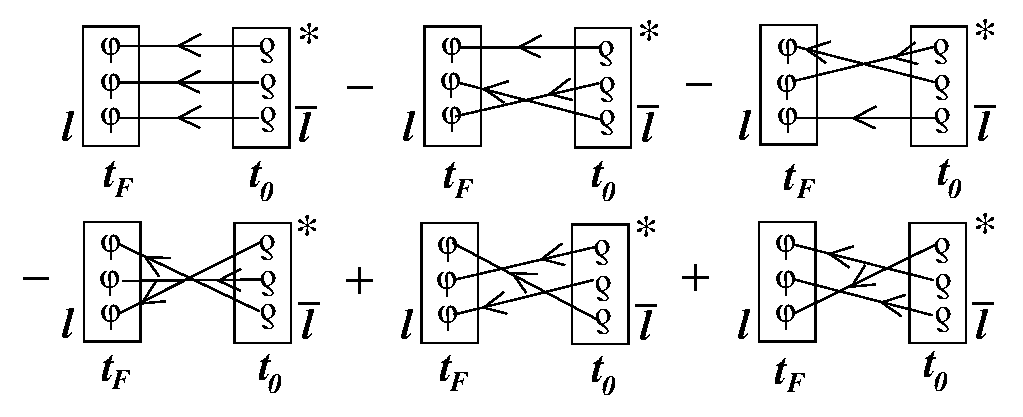
\includegraphics[width=6in]{figures/baryon_corr_diag.pdf}
    \caption[A diagrammatic representation of Eq.~(\ref{eq:corr_fac}) for a baryon correlator with source time $t_0$ and later sink time $t_F$.]{A diagrammatic representation of Eq.~(\ref{eq:corr_fac}) for a baryon correlator with source time $t_0$ and later sink time $t_F$. The boxes represent the baryon functions defined in Eq.~(\ref{eq:baryon_func}) with the first quark at the top of each box. Lines connecting a $\varrho$ to a $\varphi$ denote a summation over dilution indices. The same noise is used for both ends of any single line, and different lines use different noises. An asterisk denotes complex conjugation. Figure taken from Ref.~\cite{spectroscopy}.}
    \label{fig:baryon_corr}
\end{figure}

\chapter{Correlator Analysis: Determining the Finite-Volume Spectrum}\label{ch:analysis}
\section{Correlator Matrices}\label{sec:correlator_matrices}
In order to compute the low-lying finite-volume stationary states of QCD, we compute temporal correlator matrices of the form,
\begin{equation}
    \mathcal{C}_{i j}(t)=\bra 0 \mathcal O_{i}\left(t+t_{0}\right) \overline{\mathcal O}_{j}\left(t_{0}\right)\ket 0,
\end{equation}
where $\mathcal O_i(t+t_0)$ are the operators which annihilate the states of interest at a time $t+t_0$ and $\overline{\mathcal O}_j(t_0)$ are the corresponding operators which create the states of interest at an earlier time $t_0$. The operators are engineered such that the correlator matrix is Hermitian.\footnote{This follows from the requirement that $\bra 0 O_i \ket n = \bra n \overline O_i \ket 0 ^*$.} Since the energies are determined from the exponential decay rates of these two-point correlators, we can rescale the operators without changing the energy spectrum. In order to dampen the effects of differing normalizations among the operators, we rescale $\mathcal C(t)$ to form the actual correlator matrix $C(t)$ which we analyze as follows,
\begin{equation}
    C_{ij}(t) = \frac{\mathcal C_{ij}(t)}{\sqrt{\mathcal C_{ii}(\tau_N) \mathcal C_{jj}(\tau_N)}},
\end{equation}
where the \emph{normalization time} $\tau_N$ is taken at a very early time. Echoing the argument in Sec.~\ref{sec:intro_corr}, we can perform a spectral decomposition of $C(t)$ to obtain
\begin{equation}\label{eq:corr_spec_decomp}
    C_{i j}(t)=\sum_{n} Z_{i}^{(n)} Z_{j}^{(n) *} e^{-E_{n} t},
\end{equation}
where the $E_n < E_{n+1}$, the energies have been shifted such that $E_0\equiv 0$, and we have defined the \emph{overlap factors},
\begin{equation}
    Z_{j}^{(n) *}=\bra n \bar{O}_{j}\ket 0, \quad Z_{j}^{(n)}=\bra 0 O_{j} \ket n.
\end{equation}
The overlap factors offer us some insight into how much the state produced by a particular operator overlaps onto a particular energy eigenstate. This information can be used to make qualitative assessments of the contents of a particular energy state, e.g. if it is single- or multi-hadron dominated. Note that invariance under the a shift in phase
\begin{equation}
    Z_{j}^{(n)} \rightarrow Z_{j}^{(n)} e^{i \phi_{n}}
\end{equation}
implies that we can only determine the magnitude $|Z_j^{(n)}|$ of these overlap factors.
\section{The Generalized Eigenvalue Problem}
In the limit of infinite statistics, one could in principle fit Eq.~(\ref{eq:corr_spec_decomp}) and determine the entire energy spectrum. In practice, however, we are only able to fit the lowest one or two energies in the sum. It would be better to devise a method that allows us to fit more than just the lowest one or two energies in the spectrum. Ref.~\cite{Luscher:1990ck} proves a theorem that is the cornerstone for our approach to extracting energies from temporal correlators:
\begin{quote}
    \textbf{Theorem:} For every $t\geq 0$, 
    let $\lambda_n(t)$
    be the eigenvalues of an $N\times N$ Hermitian correlation matrix $C(t)$ ordered 
    such that
    $\lambda_0\geq \lambda_1\geq \dots\geq \lambda_{N-1}$, then 
    \begin{equation}
       \lim_{t\rightarrow\infty}\lambda_n(t)= b_n e^{-E_n t}\Bigl[1
     + \mathcal O(e^{-t\Delta_n})\Bigr],\qquad b_n>0,\quad
      \Delta_n = \min_{m\neq n}\vert E_n-E_m\vert.
    \label{eq:thmlarget}
    \end{equation}
\end{quote}
This tells us that a \emph{principal correlator} $\lambda_n(t)$ tends to a decaying exponential whose decay rate is the $n^{\rm{th}}$ energy of the spectrum. This theorem is still insufficient for use in practice, however. At large $t$ such that the $\mathcal O(e^{-t\Delta_n})$ correction is negligible, the determination of $C(t)$ has large uncertainties due to a decreasing signal-to-noise ratio~\cite{Lepage:1989hd}. At small $t$ such that $C(t)$ is well determined, the $\mathcal O(e^{-t\Delta_n})$ is not negligible. Fortunately, it is shown in Ref.~\cite{Luscher:1990ck} that the correction term can be brought down to $\mathcal O(e^{-t(E_N - E_n)})$ by instead solving the following generalized eigenvalue problem (GEVP):
\begin{equation}\label{eq:gevp}
    C(t) v_{n}\left(t, \tau_{0}\right)=\lambda_{n}\left(t, \tau_{0}\right) C\left(\tau_{0}\right) v_{n}\left(t, \tau_{0}\right), \quad n=1, \cdots, N-1, \quad \frac{t}{2} \leq \tau_0 < t.
\end{equation}
In practice, we find that a good rule of thumb to keep the $\mathcal O(e^{-t(E_N - E_n)})$ correction term low is to demand $N \geq \frac{3n}{2}$, where $n$ is the number of energies we wish to extract. Solving Eq.~(\ref{eq:gevp}) is equivalent to diagonalizing $G(t) = C^{-1 / 2}\left(\tau_{0}\right) C(t) C^{-1 / 2}\left(\tau_{0}\right)$, and the eigenvectors tend to~\cite{Blossier:2009kd}
\begin{equation}
    \lambda_{n}(t) \rightarrow\left|Z_{n}^{\prime}\right|^{2} e^{-E_{n} t}, \quad t \rightarrow \infty.
\end{equation}
The overlaps are determined by
\begin{equation}
    Z_{j}^{(n)} \approx C_{j k}\left(\tau_{0}\right)^{1 / 2} V_{k n}(t) Z_{n}^{\prime}\quad \text{(no sum over n)},
\end{equation}
where $V$ is the unitary matrix whose columns are the eigenvectors of $G(t)$.
\section{Pivots and Operator Pruning}\label{sec:pivots}
Two important assumptions about $C(t)$ are that it is Hermitian as well as positive-definite, which also implies that $G(t)$ is Hermitian and positive-definite. The assumption of positive-definiteness can be violated by operators that produce noisy correlators, or by an operator set that is linearly dependent. Noise can cause diagonal elements of the correlator to become zero or negative, and linearly dependent operators will produce eigenvalues of $C(t)$ that are zero. The odds of this occurring increases as we increase the number of operators in our correlator matrix. We call the process of judiciously choosing operators to ensure our correlator matrices remain well-conditioned \emph{pruning}. Pruning is necessary, but not sufficient for ensuring well-conditioned correlator matrices. It is still necessary to monitor for ill-conditioned matrices and take corrective action.

The condition number $\xi^{\rm{cn}}$ of a matrix is defined as the magnitude of the ratio of its maximum eigenvalue $\lambda_{\rm{max}}$ to its minimum eigenvalue $\lambda_{\rm{min}}$:
\begin{equation}
    \xi^{\rm{cn}} = \left|\frac{\lambda_{\rm{max}}}{\lambda_{\rm{min}}}\right|.
\end{equation}
When a matrix is ill-conditioned, its condition number will be high (and in some cases it may have negative eigenvalues). In order to prevent statistical noise from ruining our extraction of the energy spectrum, it is important to modify our diagonalization procedure to correct for high condition numbers, which is essentially introducing a singular value decomposition. These methods choose a threshold for the maximal allowed condition number $\xi^{\rm{cn}}_{\rm{threshold}}$ and project the correlator matrix onto the subspace spanned by the eigenvectors whose eigenvalues are larger than $\lambda_{\rm{threshold}} = \lambda_{\rm{max}}/\xi^{\rm{cn}}_{\rm{threshold}}.$ (The eigenvalues and condition numbers are all functions of $t$.)

Our entire method, which we call a pivot procedure, can be summarized as follows. Choose values for $\xi^{\rm{cn}(0)}_{\rm{max}}$, the maximal acceptable condition number for the $N\times N$ matrix $C(\tau_0)$. Let the $N_0 \leq N$ eigenvectors whose eigenvalues are greater than $\lambda^{(0)}_{\rm{max}}/\xi^{\rm{cn}(0)}_{\rm{max}}$ form the columns of the $N\times N_0$ matrix $P_0$, where $\lambda^{(0)}_{\rm{max}}$ is the largest magnitude of the eigenvalues of $C(\tau_0)$. Then define the $N_0\times N_0$ matrices
\begin{equation}
    \begin{aligned}
    \widetilde{C}\left(\tau_{0}\right)&=P_{0}^{\dagger} C\left(\tau_{0}\right) P_{0},\\
    \widetilde{C}(t)&=P_{0}^{\dagger} C(t) P_{0},\\
    \widetilde{G}(t)&=\widetilde{C}\left(\tau_{0}\right)^{-1 / 2} \widetilde{C}(t) \widetilde{C}\left(\tau_{0}\right)^{-1 / 2},
    \end{aligned}
\end{equation}
for $t\neq t_0$. We then solve for the eigenvectors and eigenvalues of $\widetilde G(t)$. Let the $N_P\leq N_0$ eigenvectors whose eigenvalues are greater than $\lambda^{(t)}/\xi^{(t))_{\rm{max}}}$ form the columns of the $N_0\times N_P$ matrix $\widetilde V(t)$, where $\lambda^{(t)}_{\rm{max}}$ is the largest magnitude of the eigenvalues of $\widetilde G(t)$. The $N_P\times N_P$ matrix
\begin{equation}
    \widetilde{\Lambda}(t)=\widetilde{V}^{\dagger}(t) \widetilde{G}(t) \tilde{V}(t)
\end{equation}
will satisfy
\begin{equation}
    \begin{aligned}
    &\widetilde{\Lambda}\left(\tau_{0}\right)=I,\\
    &\widetilde{\Lambda}(t)=\operatorname{diag}\left(\lambda_{n}(t)\right),
    \end{aligned}
\end{equation}
where $\lambda_n \rightarrow \left|\widetilde{Z}_{n}^{\prime}\right|^{2} e^{-E_{n} t}$ for large $t$ and $Z_{i}^{(n)} \approx P_{0 i j} \widetilde{C}_{j k}\left(\tau_{0}\right)^{1 / 2} \widetilde{V}_{k n}(t) \widetilde{Z}_{n}^{\prime}$. We can therefore fit the different $\lambda_n(t)$ for energies and overlap factors of the spectrum. The pivot method presented above involves rotating the correlator at every time slice, but in practice, this is not strictly necessary. We can instead take a simpler approach of diagonalizing $\widetilde G(t)$ at only one time $\tau_d$ chosen such that $\tau_d > \tau_0$, and using the same matrix to diagonalize at every other time, provided that the off-diagonal elements are statistically consistent with zero for all time slices $t \geq \tau_d$. Using the same transformation at every time slice is an ingredient in the \emph{single pivot} method, and is the procedure used in this work. Note that choosing $\tau_d \approx 2\tau_0$ ensures minimal contamination from higher lying states~\cite{Luscher:1990ck}.
\subsection{The Zero Temperature Assumption}
An important caveat to everything presented thus far is that we work in the assumption of a zero-temperature (i.e. infinite time extent) limit. Recall that the expression relating two-point correlators to a sum of decaying exponentials, given by Eq.~(\ref{eq:corr_decomp}) rests on the assumption that $t\ll T$, where $T$ is the time extent of the lattice. When calculating correlator matrix elements, this should be corrected to
\begin{equation}\label{eq:corr_thermal}
    \begin{aligned}
        \mathcal{C}_{i j} &=\left\langle\mathcal{O}_{i}(t) \overline{\mathcal{O}}_{j}(0)\right\rangle_{T} \\
        &=\frac{1}{Z_{T}} \operatorname{Tr}\left[e^{-H T} \mathcal{O}_{i}(t) \overline{\mathcal{O}}_{j}(0)\right] \\
        &=\frac{1}{Z_{T}} \sum_{n}\bra n e^{-H(T-t)} \mathcal{O}_{i}(0) e^{-H t} \overline{\mathcal{O}}_{j}(0)\ket n \\
        &=\frac{1}{Z_{T}} \sum_{n, m} e^{-E_{n}(T-t)} e^{-E_{m} t}\bra n \mathcal{O}_{i}(0)\ket m \bra m \overline{\mathcal{O}}_{j}(0)\ket n,
        \end{aligned}
\end{equation}
where
\begin{equation}
    \begin{aligned}
        Z_{T} & = \operatorname{Tr} e^{-H T} \\
        &=\sum_{n}\bra n e^{-H T}\ket n \\
        &=\sum_{n} e^{-E_{n} T}.
    \end{aligned}
\end{equation}
Only in the limit $T\rightarrow \infty$ does Eq.~(\ref{eq:corr_thermal}) agree with Eq.~(\ref{eq:corr_decomp}) and Eq.~(\ref{eq:corr_spec_decomp}). The thermal effects of finite time extent will manifest as backwards propagating modes which will be briefly discussed in Sec.~\ref{sec:fit_forms}. Fortunately, on the $32^3\times 256$ anisotropic lattice used in this work, these thermal effects (or temporal wrap-around effects) are negligible, and even on smaller lattices, we only find it necessary to account for backwards propagating modes for the lightest states.
\section{Fit Forms}\label{sec:fit_forms}
Fitting the diagonalized correlators is accomplished by forming fit ansatzes based on decaying exponentials, or symmetric exponentials when we wish to account for thermal effects. One such fit form is the single exponential,
\begin{equation}\label{eq:single_exp}
    C(t) = Ae^{-E t}.
\end{equation}
This form is strictly incorrect for finite $t$ due to excited state contamination (i.e. subleading exponential contributions from higher-lying states), but it is approximately correct for sufficiently large $t$. The single exponential has the advantage that it has few fit parameters and is thus less sensitive to statistical noise, but it has the disadvantage that it is highly sensitive to the minimum time in the used in the fit domain. The fit domain must only include times at which the subleading contributions are negligible.

We can account for the effects of higher-lying states by using a two-exponential fit,
\begin{equation}
    C(t)=A e^{-E t}\left(1+B e^{-\Delta^{2} t}\right),
\end{equation}
where the term $\Delta^2$ is used to ensure that the gap to the next energy is positive. We can also attempt to account for higher-lying states by using an ansatz that mocks up these states as a sum of equally-spaced levels above the fit energy $E$:
\begin{equation}
    C(t)=\frac{A e^{-E t}}{1-B e^{-\Delta^{2} t}} = Ae^{-Et}\left(\sum_{n=0}^\infty B^n e^{-\Delta^{2n}t}\right).
\end{equation}
These forms have the advantage that they are less sensitive to the fit domain and more accurately model the theory, but they have the disadvantage that they contain more parameters and are more sensitive to statistical noise. For this reason, we must often resort to using a single-exponential fit for noisier correlators.

If we wish to account for thermal effects for mesons, we can also make any fit form symmetric, e.g.
\begin{equation}
    C(t)=A\left(e^{-E t}+e^{-E(T-t)}\right)
\end{equation}
for the single exponential fit form. For baryons, things become more complicated, since the backwards propagating mode actually corresponds to a baryon's parity partner, which would necessitate fitting in two symmetry channels simultaneously. Fortunately, baryons are heavy enough that accounting for temporal wrap-around effects is usually not necessary. Note that no extra parameters are needed for this, so it is easy to verify if such fit forms are necessary. Additionally, a constant can be added to any of the fit forms to help account for vacuum expectation values and to account for thermal effects on smaller lattices.
\subsection{The Effective Energy}\label{sec:eff_mass}
A very useful tool in fitting correlators is the so-called \emph{effective energy} or \emph{effective mass} which is given by
\begin{equation}
    E_{\rm{eff}}(t) = -\frac{d}{dt}\ln C(t),
\end{equation}
which can be discretized and estimated as
\begin{equation}
    -\frac{1}{\Delta t}\left(\ln C(t+\Delta t)-\ln C(t)\right).
\end{equation}
The effective energy is designed such that it tends to the fit energy $E$ as $t\rightarrow \infty$. When performing our fits, we are usually visually guided by effective energy plots rather than the correlators themselves, but it is crucial to emphasize that we do not fit the effective energy itself. An example of an effective energy plot is given in Fig.~(\ref{fig:eff_en_ex}). (will include plot when results are finalized.)
\section{Error Analysis and Resampling}
The observables we estimate through direct Monte Carlo measurements on gauge configurations are called \emph{simple} observables. Estimating the variance of simple observables is straightforward via calculating the population variance using the Monte Carlo method. All other observables are called \emph{non-simple} observables. An example of a non-simple observable is a model parameter obtained when we fit a correlator to data points which are themselves averages over many gauge configurations. The way to approach error analysis for non-simple observables is through \emph{resampling} techniques. Resampling involves forming new datasets from an initial dataset in order to estimate properties of how that dataset is distributed. For example, if we wanted to estimate the variance of the mean of some variable $x$, we would need several sets of measurements $\{x\}_i$ from which we can estimate the variance of the mean as
\begin{equation}
    \sigma^2_{\overline x} = \langle  \overline x^2 \rangle  - \langle \overline x \rangle ^2,
\end{equation}
where $\overline x$ denotes the population mean of a single set, and $\langle\rangle$ denotes the average over all populations $\{x\}_i$. In general, we wish to inquire about any arbitrary property of a set $\{x\}$. When only one dataset $\{x\}$ is available, resampling can be used to form new sets $\{x\}_i$ using only the original set. The dataset we consider is a set of gauge configurations $\{U\}$. Here we outline two resampling techniques, namely the \emph{jackknife} and the \emph{bootstrap}~\cite{efron1982jackknife}.

Jackknife resampling proceeds as follows. For a set of $N_c$ configurations $\{U\}$, form new sets $\{U\}_i$ which consist of every configuration in $\{U\}$ \emph{except} for the $i^{\rm{th}}$ configuration. There will be $N_c$ such new sets, and we expect that because only one configuration has been removed from each, that any properties we measure of the set will be close to those of the original set.

Bootstrap resampling proceeds as follows. For a set of $N_c$ configurations $\{U\}$, form $N_b$ new sets $\{U_i\}$ by choosing $N_c$ configurations from $\{U\}$ randomly with replacement. Since configurations can be sampled multiple times or not at all, we do not expect that properties we measure of the resampled sets will necessarily be distributed closely to that of the original set, as we do with jackknife resampling.

The properties we wish to estimate are the covariances of our model fit parameters, such as the energies and overlap factors. For jackknife resampling, we estimate the covariance as
\begin{equation}
    \operatorname{cov}(f_i, f_j) = \frac{N_c - 1}{N_c}\sum_{i=1}^{N_c}\left(\langle f \rangle_i - \langle f \rangle^J\right)\left(\langle f \rangle_j - \langle f \rangle^J\right),
\end{equation}
where $\langle f \rangle_i$ denotes the average of $f$ over the $i^{\rm{th}}$ jackknife resampling, and $\langle f \rangle^J$ denotes the average of $f$ over all resamplings. For bootstrap resampling, we estimate the covariance as
\begin{equation}
    \operatorname{cov}(f_i, f_j) = \frac{1}{N_b-1}\sum_{i=1}^{N_b}\left(\langle f \rangle_i - \langle f \rangle^B\right)\left(\langle f \rangle_j - \langle f \rangle^B\right),
\end{equation}
where $\langle f \rangle_i$ denotes the average of $f$ over the $i^{\rm{th}}$ bootstrap resampling, and $\langle f \rangle^B$ denotes the average of $\langle f \rangle_i$ over all bootstrap resamplings.
\section{Correlated $\chi^2$ Minimization}
For uncorrelated data, it is usually sufficient to fit the model parameters $\bs \alpha$ of a function $f(t;\bs \alpha)$ correlater data $C(t)$ by minimizing the uncorrelated $\chi^2$ metric defined by
\begin{equation}
    \chi^{2}=\sum_{t} \frac{(C(t)-f(t;\bs\alpha))^{2}}{\sigma_{t}^{2}},
\end{equation}
where $\sigma_t^2$ is the variance of the data at each time point. Our measurements are not statistically independent, however, because each measurement is taken on the same set of gauge configurations. We must therefore fit our correlators by instead minimizing the correlated $\chi^2$, defined by
\begin{equation}\label{eq:corr_chisq}
    \chi^{2}= \sum_{t,t^\prime} = \left(C(t) - f(t;\bs\alpha)\right)\operatorname{cov}^{-1}\left(C(t), C(t^\prime)\right)\left(C(t^\prime) - f(t^\prime; \bs\alpha)\right).
\end{equation}
The model parameters are then fit by minimizing $\chi^2$ on each resampling and calculating their uncertainties using the relevant covariance formula for the given resampling scheme.

% \chapter{Scattering Resonances in a Two-Scalar Field Theory}
% $\phi/\rho$


\chapter{Investigating the Tetraquark Content of the Light Scalar Mesons $\kappa$ and $a_0(980)$}\label{ch:tetraquarks}
In this chapter, we examine the effect of including tetraquark operators on the spectrum determination in the scalar meson sectors containing the $K_0^*(700)$ (previously the $K_0^*(800)$, here and often elsewhere referred to as the $\kappa$) and the $a_0(980)$. It has been suggested before that the $\kappa$ and $a_0(980)$ could have tetraquark content~\cite{Jaffe:2004ph, Amsler:2004ps, Close:2002zu, Maiani:2004uc}, and to date, there have been a small number of studies investigating tetraquarks on the lattice using light quarks. In 2010, Prelovsek et al.\ investigated the $\sigma$ and $\kappa$ as possible tetraquark candidates, but neglected disconnected diagrams in their calculations~\cite{Prelovsek:2010kg}. Using tetraquark interpolators, they found an additional light state in both the $\sigma$ and $\kappa$ channels. In 2013, the ETM collaboration examined the $a_0(980)$ and $\kappa$ using four-quark operators~\cite{Alexandrou:2012rm}, though they also neglected disconnected diagrams in their calculations. They found no evidence of an additional state that can be interpreted as a tetraquark. In 2018, Alexandrou et al.\ conducted a study of the $a_0(980)$ with four-quark operators~\cite{Alexandrou:2017itd}, including disconnected contributions. In their study, they found an additional finite-volume state in the sector containing the $a_0(980)$ meson, which has primarily quark-antiquark content but also has sizeable diquark-antidiquark content, in the range of 1100 to 1200 MeV. Additionally, they conclude that disconnected diagrams have drastic effects on their results, and thus cannot be neglected. We make two different determinations of the spectrum in each symmetry channel: one using a basis of only single- and two-meson operators, and one using a basis that also includes a tetraquark operator selected from hundreds of tetraquark operators which were tested. We find that including a tetraquark operator yields an additional low-lying finite-volume state in each symmetry channel. In this work, we use the stochastic LapH method~\cite{Morningstar:2011ka} to evaluate the diagrams in our calculations, including \textit{all} disconnected contributions.
\section{Ensemble}\label{sec:ensemble}
We perform Monte Carlo calculations using $412$ gauge field configurations generated by the Hadron Spectrum collaboration~\cite{Edwards:2008ja, Lin:2008pr} on an anisotropic lattice of size $32^3\times 256$ with a length of $3.74$ fm and a pion mass of approximately $230$ MeV, using $N_f=2+1$ Wilson clover fermions. Ensemble details are given in Table~\ref{table:ensemble}, and the action is described in Sec.~\ref{sec:improved_action} and Sec.~\ref{sec:tuning}.
\renewcommand{\arraystretch}{1.0}
\begin{table}
  \centering
  \begin{tabular}{|l|l|l|l|l|l|}
    \hline
    $(L/a_s)^3 \times (T/a_t)$ & $N_{\rm{configurations}}$ & $a_t m_\pi$ & $a_t m_K$ & $a_t$ & $\xi$ \\
    \hline
    $32^3\times 256$ & $412$ & $0.03953(17)$ & $0.08348(14)$ & $0.033357(59)$ fm & $3.451(11)$\\
    \hline
  \end{tabular}
  \caption{Details of the ensemble used in this work. The temporal lattice spacing is taken from Ref.~\cite{Brett:2018jqw}. The renormalized anisotropy $\xi$ is taken from Ref.~\cite{Bulava:2016mks}.}\label{table:ensemble}
\end{table}
\renewcommand{\arraystretch}{1.5}
\section{Operator Construction}
We include single- and two- meson operators, as well as tetraquark operators, in the basis of interpolating operators. As a brief review of the material presented in Ch.~\ref{ch:operators}, we construct our elemental operators using building blocks of smeared, gauge-covariantly displaced quark fields, and stout-smeared link variables. To form the final operators out of our elemental operators, we project the elemental operators onto various symmetry channels according to isospin, parity, $G$-parity, octahedral little group, etc. That is, to form a meson operator $M_{l}(t)$ that transforms irreducibly under all symmetries of interest (labeled by the compound index $l$) at time $t$, we must 
take a linear combination of our elemental meson operators, $M_{l}(t)=c_{\alpha \beta}^{(l)} \Phi_{\alpha \beta}^{A B}(\boldsymbol{p}, t)$. To form a two-meson operator $\mathcal{O}_l(t)$, we would follow a similar procedure and project the product of two final meson operators $M^{a}_{l_a}(t) M^{b}_{l_a}(t)$ onto a final symmetry channel $l$: $\mathcal{O}_l(t) = c^{(l)}_{l_a l_b} M^{a}_{l_a}(t) M^{b}_{l_a}(t)$.

Recall that in order to construct a tetraquark operator, we must consider the various ways to construct a color-singlet four-quark object out of four quark fields. As seen in Ref.~\cite{pittir33243}, the Clebsch-Gordon decompositions show that the only way to construct a color-singlet is by using two quarks and two antiquarks, and that doing so yields two linearly independent color singlet objects:
\begin{equation}\label{eq:cg}
\begin{array}{l}
    {3 \otimes 3 \otimes 3 \otimes 3=3\oplus3\oplus3\oplus\overline{6}\oplus\overline{6}\oplus15\oplus15\oplus15\oplus15},\\
    {3 \otimes 3 \otimes 3 \otimes \overline{3}=\overline{3}\oplus\overline{3}\oplus\overline{3}\oplus6\oplus6\oplus6\oplus\overline{15}\oplus\overline{15}\oplus24},\\
    {3 \otimes 3 \otimes \overline{3} \otimes \overline{3}=1\oplus1\oplus8\oplus8\oplus8\oplus8\oplus10\oplus\overline{10}\oplus27}.
\end{array}
\end{equation}
There are 81 basis vectors formed by the quark fields, $p_{a}^{*}(x) q_{b}^{*}(x) r_{c}(x) s_{d}(x)$, where each $r$, $s$ transforms as a color vector in the fundamental $3$ irrep, and so, $p^{*}$, $q^{*}$ transform in the $\overline 3$ irrep. The following combinations are both linearly independent and gauge-invariant,
\begin{equation}\label{eq:tsta}
\begin{aligned} T_{S} &=\left(\delta_{a c} \delta_{b d}+\delta_{a d} \delta_{b c}\right) p_{a}^{*}(x) q_{b}^{*}(x) r_{c}(x) s_{d}(x), \\ T_{A} &=\left(\delta_{\alpha c} \delta_{b d}-\delta_{\alpha d} \delta_{b c}\right) p_{\alpha}^{*}(x) q_{b}^{*}(x) r_{c}(x) s_{d}(x),\end{aligned}
\end{equation}
and so they form a basis with which to construct our elemental tetraquark operators, fulfilling the need for \emph{two} linearly independent color singlet operators from Eq.~(\ref{eq:cg}).

While we chose only a handful of tetraquark operators for our final analysis, we designed hundreds of operators with differing flavor structures, color structures (i.e. the symmetric and antisymmetric combinations of Eq.~(\ref{eq:tsta})), and displacements. We tested these operators by individually adding them to a basis of single- and multi-meson operators to see if an additional level was found in an initial low-statistics analysis on 25 gauge configurations. Most of the operators did not yield an additional level, but we found particular operators that did. In the $\kappa$ channel, we tested the following flavor structures: $\overline s u \overline s s$, $\overline s u \overline u u$, and $\overline s u \overline d u$. We found that only operators with the $\overline s u \overline s s$ flavor structure yielded an additional finite-volume state, and that the additional state was present with both color structures. In our initial low-statistics analysis, we tested both single-site and quadruple displacements, and found operators of both types that seemed to yield additional finite-volume states; however, the quadruply-displaced operators came at a significantly higher computational cost and introduced either additional noise or no improvement, and so were excluded from the final operator sets. In the $a_0(980)$ channel, we tested the following flavor structures: $\overline u u \overline d u$, $\overline s s \overline d u$, and $\overline d u \overline d u$. We found that only operators with the $\overline u u \overline d u$ flavor structure yielded an additional finite-volume state. As in the $\kappa$ channel, we found that both color structures were able to produce an additional level. After finding no improvement with other displacement types in the $\kappa$ channel, we chose to only test single-site operators in the $a_0(980)$ channel. In both channels, we also constructed operator bases that included several tetraquark operators, and found that the number of additional levels in the energy range we examined was unchanged.

\section{$\kappa$ Channel}
\subsection{Operator Bases}
The quantum numbers associated with the $\kappa$ are $I(J^{P})=\frac{1}{2}(0^+)$ and $S=-1$ , which means that on the lattice we work in the isodoublet, strange, $A_{1g}$ symmetry sector (see Table~\ref{table:O_occurrence_nums}). Below a cutoff of approximately 1.5 times the mass of the nucleon, where the $K_0^*(1430)$ resonance is expected, we expect to see only multi-hadron states. Since we are examining the effect of tetraquark operators on just the low-lying states, we therefore primarily include two-hadron operators. It is always a good idea to add one or more single hadron operators, however, as any operator with the correct quantum numbers can excite states in the spectrum. The operator basis we use, not including any tetraquark operators, is shown in Table~\ref{table:kappa_ops_no_tq}.
\begin{table}
  \centering
  \begin{tabular}{l|l}
    \textbf{Single-Hadron Operators} & \textbf{Two-Hadron Operators}\\
    \hline
    $K^{\rm{DDL}5}_{A_{1g}}$ & $K(0)^{\rm{SS}0}_{A_{1u}}\; \pi(0)^{\rm{SS}0}_{A_{1u}^+}$\\
    $K^{\rm{TDO3}5}_{A_{1g}}$ & $K(0)^{\rm{SS}0}_{A_{1u}}\; \eta(0)^{\rm{SS}0}_{A_{1u}^+}$ \\
    $K^{\rm{TDU}5}_{A_{1g}}$ & $K(0)^{\rm{SS}0}_{A_{1u}}\; \phi(0)^{\rm{SS}0}_{A_{1u}^+}$ \\
    & $K(1)^{\rm{SS}1}_{A_2}\; \pi(1)^{\rm{SS}1}_{A_2^-}$ \\
    & $K(1)^{\rm{SS}1}_{A_2}\; \eta(1)^{\rm{SS}1}_{A_2^+}$ \\
    & $K(1)^{\rm{SS}1}_{A_2}\; \phi(1)^{\rm{SS}1}_{A_2^+}$ \\
    & $K(2)^{\rm{SS}0}_{A_2}\; \pi(2)^{\rm{SS}0}_{A_2^-}$ \\
    & $K(3)^{\rm{SS}0}_{A_2}\; \pi(3)^{\rm{SS}0}_{A_2^-}$
  \end{tabular}
  \caption{Operators used in the $\kappa$ channel, excluding tetraquark operators. Particle names refer to \emph{flavor content} and should not be taken literally. $K$ refers to $u\overline s$, $\pi$ refers to $u\overline d$, $\eta$ refers to $u\overline u + d\overline d$, and $\phi$ refers to $s\overline s$ flavor structure. The number in parentheses following the particle name denotes the square of its total momentum in lattice units, the superscript denotes displacement type, and the subscript denotes octahedral irrep and $G$-parity.}
  \label{table:kappa_ops_no_tq}
\end{table}

Our final class of tetraquark operators used in this channel were single-site $\overline s u \overline s s$, with both the symmetric and antisymmetric color structures included. The final tetraquark operator chosen was a $\overline s u \overline s s$, antisymmetric, single-site operator, which we denote as \verb+tqsuss2m SS2+. Of the tetraquark operators that produced an additional level, we chose this one due to its high signal quality.
\subsection{Spectrum Determination}
For all results in this chapter, we use the kaon mass as a reference. The fit used to determine the kaon mass is shown in Fig.~\ref{fig:kaon}. For all fits in this channel, the normalization time, metric time, and diagonalization time used in the GEVP were $\tau_N=3$, $\tau_0=6$, and $\tau_d=12$, respectively. While we expect that the single-pivot method described in Sec.~\ref{sec:pivots} ensures that the correlator matrix remains diagonal at all times, it is sometimes difficult to ensure that off-diagonal elements of the correlator matrix are statistically consistent with zero at all times. Choosing later diagonalization times helps with this, but comes with the tradeoff of introducing more noise. We found that choosing $\tau_d=12$ yielded a good combination of reduced noise and a near-sufficiently diagonal matrix. Still, there were some off-diagonal elements which were slightly farther than zero than we would hope, so we took care to extract the spectrum at three different diagonalization times and confirm that our energies were consistent across these diagonalization times. Our results are shown in Fig.~\ref{fig:spectrum_td}.

Fits to the diagonalized correlator set for the operator basis containing no tetraquark operators are shown in Fig.~\ref{fig:kappa_no_tq_grid}, and the operator overlap factors are shown in Fig.~\ref{fig:kappa_no_tq_zfactors}. Fit details are given in Table~\ref{table:kappa_no_tq_spectrum}. Recall from Sec.~\ref{sec:correlator_matrices} that we must use more operators in our basis than energies we wish to reliably extract, so there are fewer fits shown than operators used. (This will often be the case throughout this work.) Fits using the same operator basis, but with the addition of the $\overline s u \overline s s$ tetraquark operator, are shown in Fig.~\ref{fig:kappa_with_tq_grid}, and the operator overlap factors are shown in Fig.~\ref{fig:kappa_with_tq_zfactors}. Fit details are given in Tables~\ref{table:kappa_with_tq_spectrum}. We prefer to use two-exponential fits wherever possible, though it is sometimes necessary to use single-exponential fits to achieve precise energy determinations. We choose the beginning of the fit range $t_{\rm{min}}$ by fitting to several values and choosing the earliest value at which the fit value becomes stable, in order to determine when excited state contamination stops altering our result. The end of the fit range $t_{\rm{max}}$ is chosen to be approximately the time at which the principle correlator becomes statistically consistent with zero, since fitting to points with a low signal-to-noise ratio is undesirable.

A plot comparing our determinations of the low-lying spectrum for each basis is shown in Fig~\ref{fig:kappa_spectrum}. The result is clear: including the tetraquark operator yields an additional level at $E/m_K = 2.139(62)$. Without including such a tetraquark operator, we miss an energy level in the spectrum determination. Additionally, we see that the energy determinations for the other levels shift slightly, which is to be expected when one attempts to extract a spectrum with an operator basis that is not sufficiently saturated with operators.~\cite{Dudek:2012xn} Taking a look at the overlap factors, we see that there is significant overlap between this additional level and the state created by the tetraquark operator. This significant result suggests that there is a state in the finite-volume lattice spectrum that shares quantum numbers with the $\kappa$ resonance, and that has tetraquark content.

Firm evidence of the $\kappa$ resonance having tetraquark content will have to wait for future scattering studies employing L\"uscher's method~\cite{Luscher:1990ck}, which is a formalism that relates discrete finite-volume spectra to infinite-volume scattering amplitudes. It is worth noting that one such study of the $\kappa$ resonance by Brett et al.~\cite{Brett:2018jqw}, using the same ensemble used here, gave a qualitative determination of the $\kappa$ mass to be $4.66(11)m_\pi$ from an effective range parameterization and $4.59(11)m_\pi$ from  a Breit-Wigner parameterization. Both of these masses are within error of the mass of our additional finite-volume state, which is $4.52(13)m_\pi$ (the pion mass fit used to determine this ratio is shown in Fig.~\ref{fig:pion}). Additionally, the consequences of missing a finite-volume energy such as the one found in this work may be severe for variants of L\"uscher's method that fit scattering parameters by comparing the finite-volume spectrum predicted by a particular scattering amplitude to that obtained on the lattice, such as the method used by the Hadron Spectrum Collaboration in Ref.~\cite{Wilson:2015dqa}. However, for variants of L\"uscher's method that rely on computing scattering parameters from finite-volume energies, such as the determinant residual method~\cite{Morningstar:2017spu} used by Brett et al.\, the consequences should not be as severe.

\begin{figure}
  \centering
  \begin{subfigure}{0.4\textwidth}
    \centering
    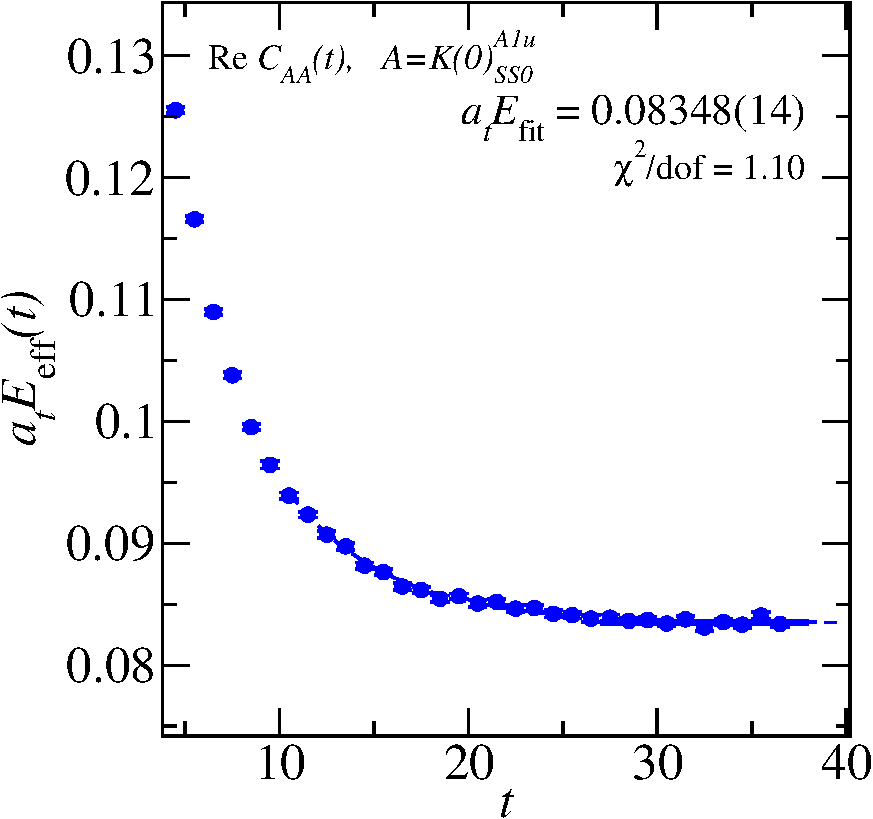
\includegraphics[width=\textwidth]{figures/kaon_crop.pdf}
    \caption{Kaon mass}\label{fig:kaon}
  \end{subfigure}\hfill
  \begin{subfigure}{0.4\textwidth}
    \centering
    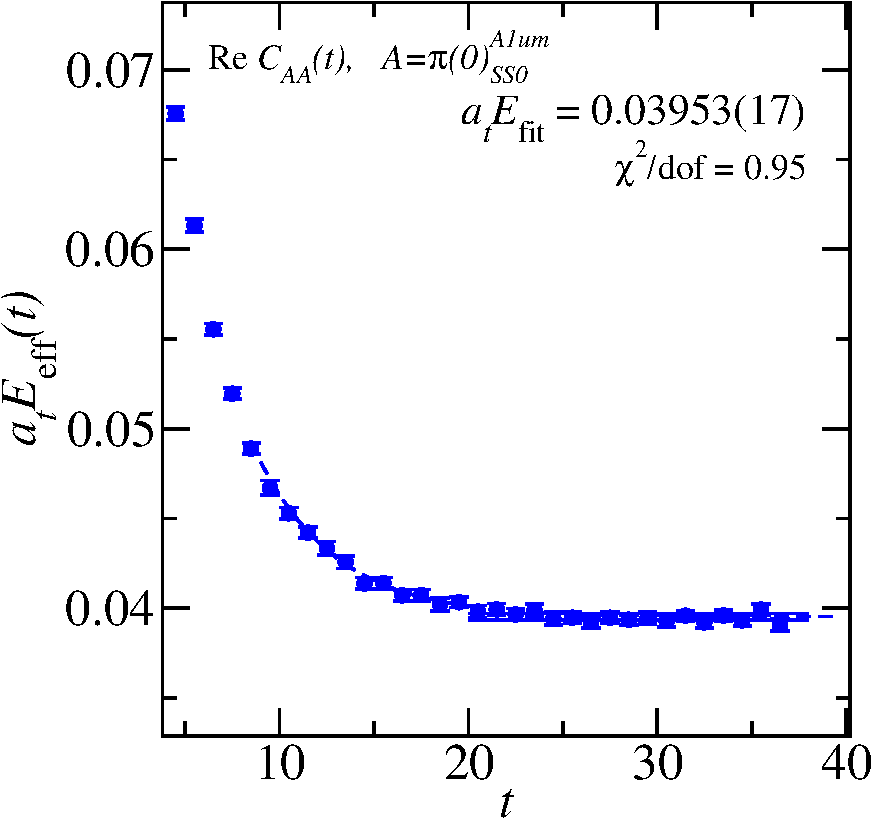
\includegraphics[width=\textwidth]{figures/pion_crop.pdf}
    \caption{Pion mass}\label{fig:pion}
  \end{subfigure}
  \caption{Fits to the reference masses, used in this chapter.}
\end{figure}

\begin{figure}
  \centering
  \hspace*{-0.5in}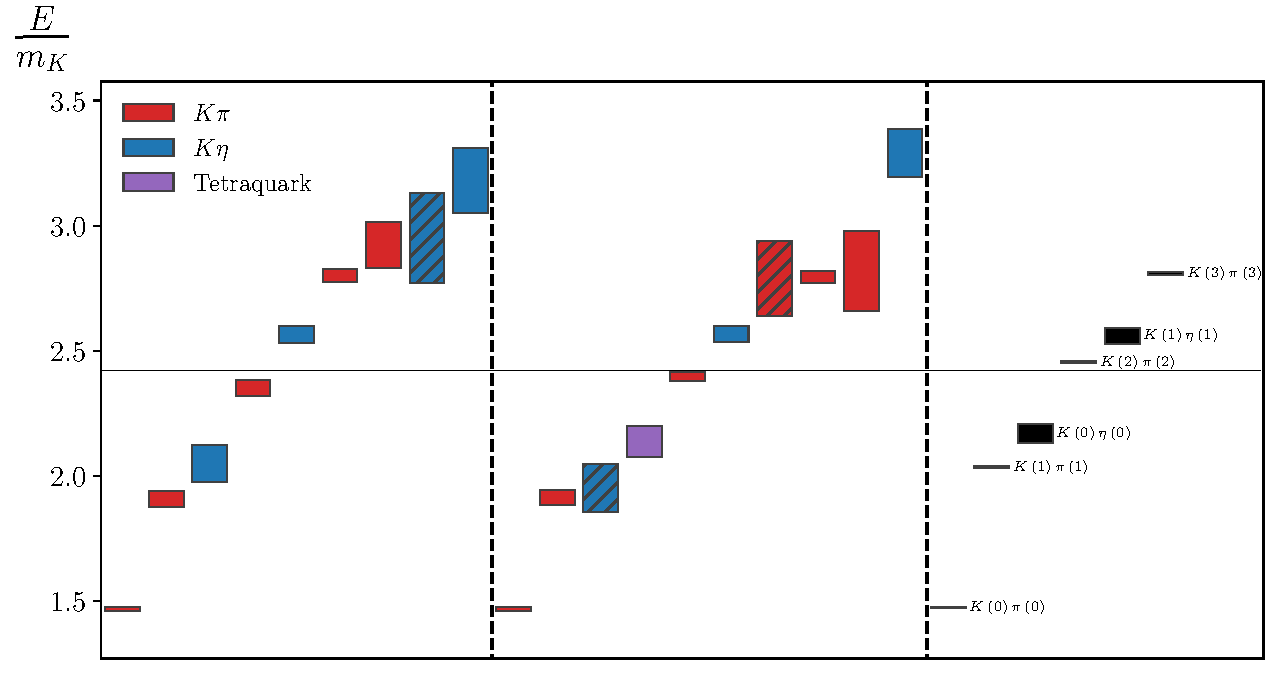
\includegraphics[width=\textwidth]{figures/spectrum_a1g/staircase.pdf}
  \caption{On the left: a spectrum obtained in the $\kappa$ channel using the operator basis given in Table~\ref{table:kappa_ops_no_tq}, which contains no tetraquark operators. In the middle: a spectrum obtained in the $\kappa$ channel using the same basis but with the addition of one tetraquark operator. On the right: two-particle non-interacting energies calculated from the rest-frame masses of the constituent particles, up to the point at which we have confidently saturated the basis with two-particle operators. The horizontal dashed line indicates the four-particle $K\pi\pi\pi$ threshold. The color of a level indicates flavor content, determined by finding which operator has the largest overlap factor with that level. If the level has significant overlap with more than one operator (with the smaller overlap being $\geq 70\%$ of the larger overlap), then a hatched box is used to denote significant mixing.}
  \label{fig:kappa_spectrum}
\end{figure}

\begin{figure}
  \centering
  \hspace*{-0.5in}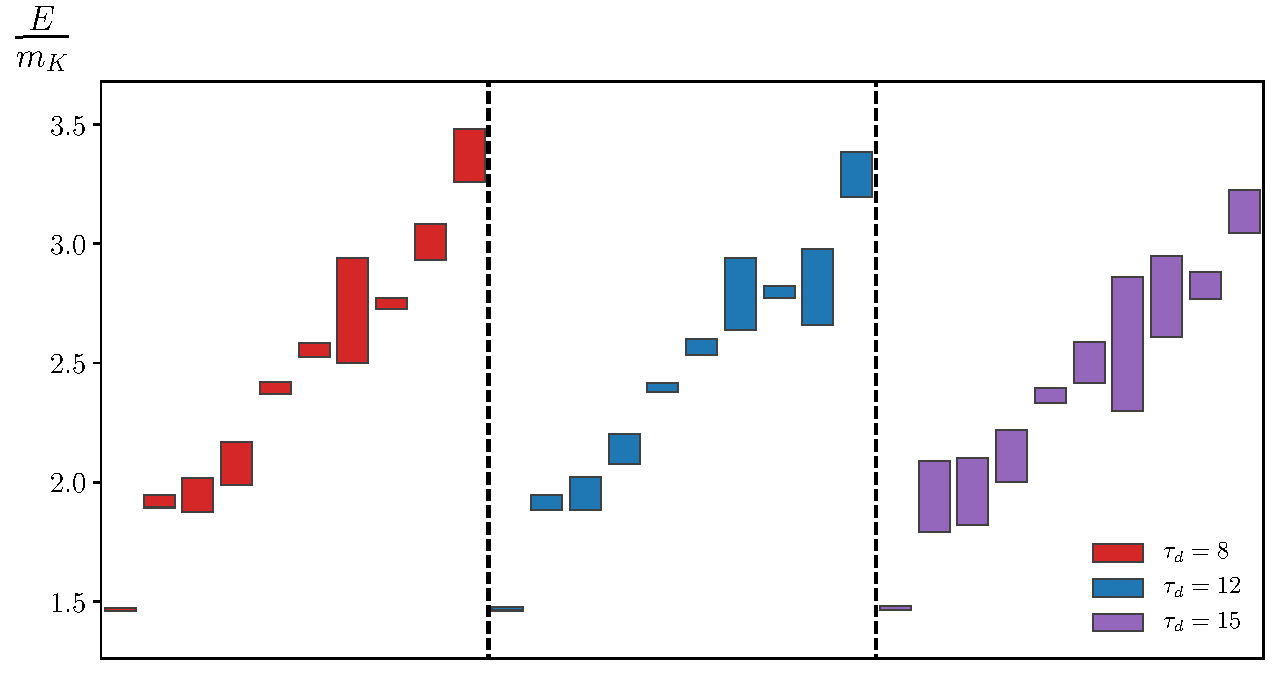
\includegraphics[width=\textwidth]{figures/spectrum_a1g/staircase_tau_d.pdf}
  \caption{The spectrum obtained using three different diagonalization times, using the operator basis given in Table~\ref{table:kappa_ops_no_tq} with the addition of the $\overline s u \overline s s$ tetraquark operator.}
  \label{fig:spectrum_td}
\end{figure}

\begin{figure}
  \raisebox{-.08cm}{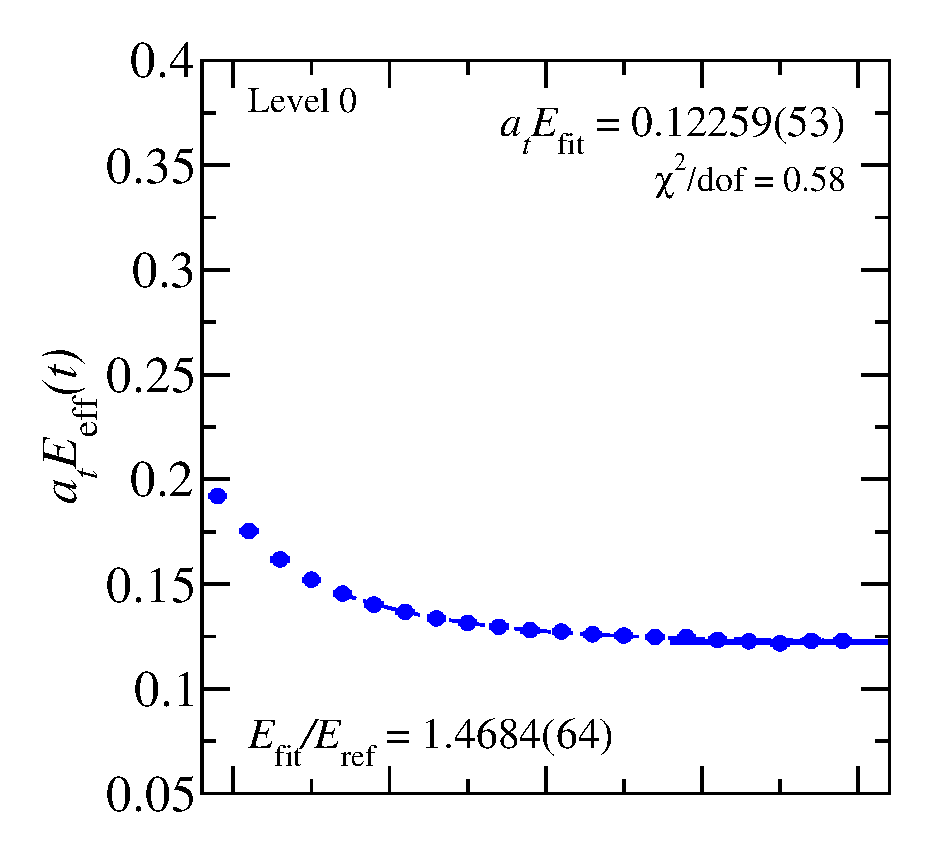
\includegraphics[width=0.336\textwidth]{figures/spectrum_a1g/no_tq/fits/fit_0.pdf}}
  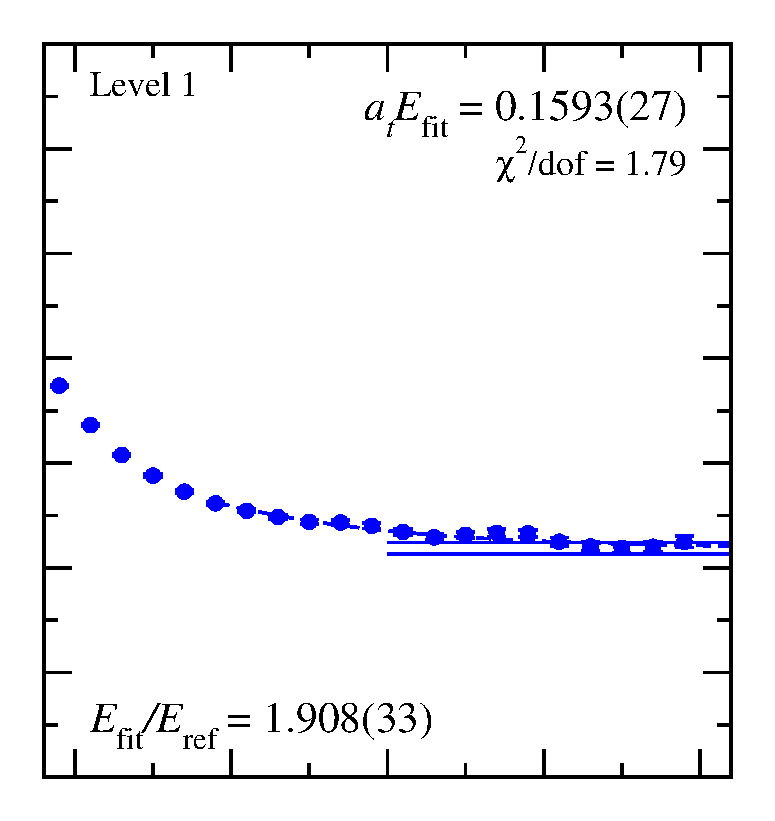
\includegraphics[width=0.28\textwidth]{figures/spectrum_a1g/no_tq/fits/fit_1.pdf}
  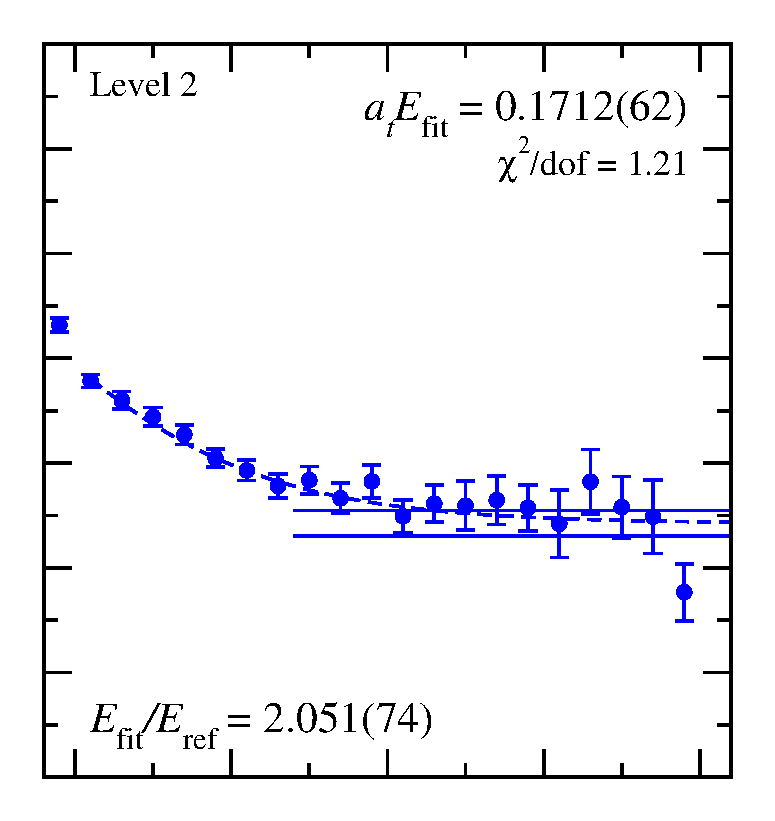
\includegraphics[width=0.28\textwidth]{figures/spectrum_a1g/no_tq/fits/fit_2.pdf}\\
  \raisebox{-.08cm}{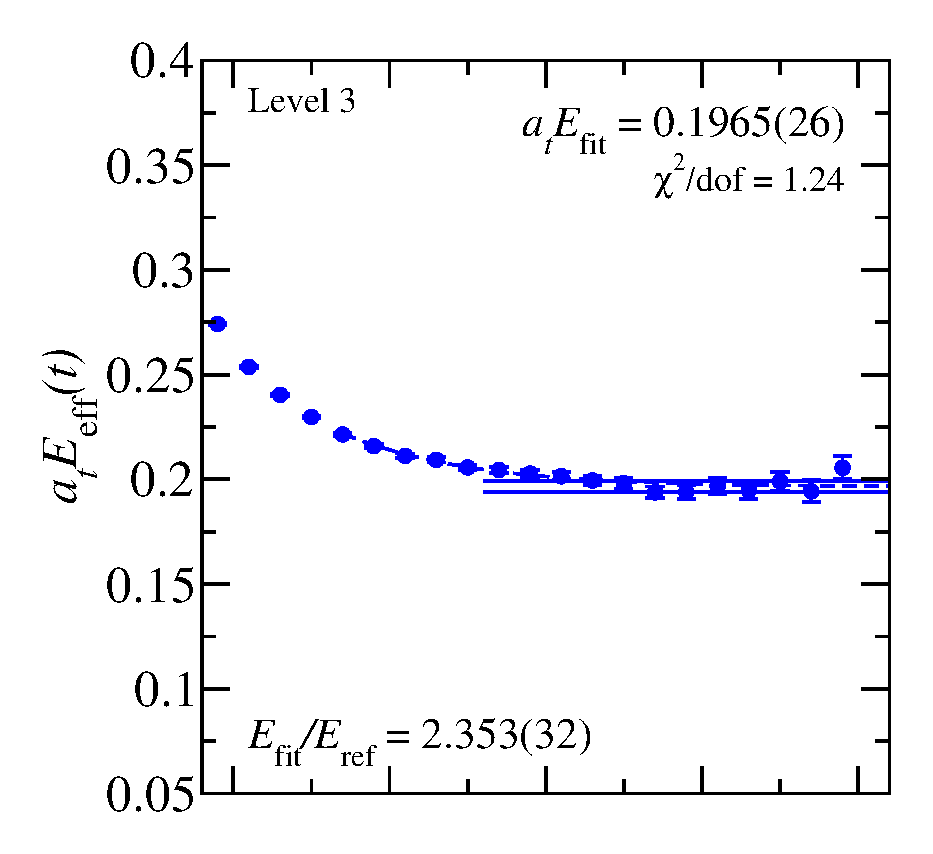
\includegraphics[width=0.336\textwidth]{figures/spectrum_a1g/no_tq/fits/fit_3.pdf}}
  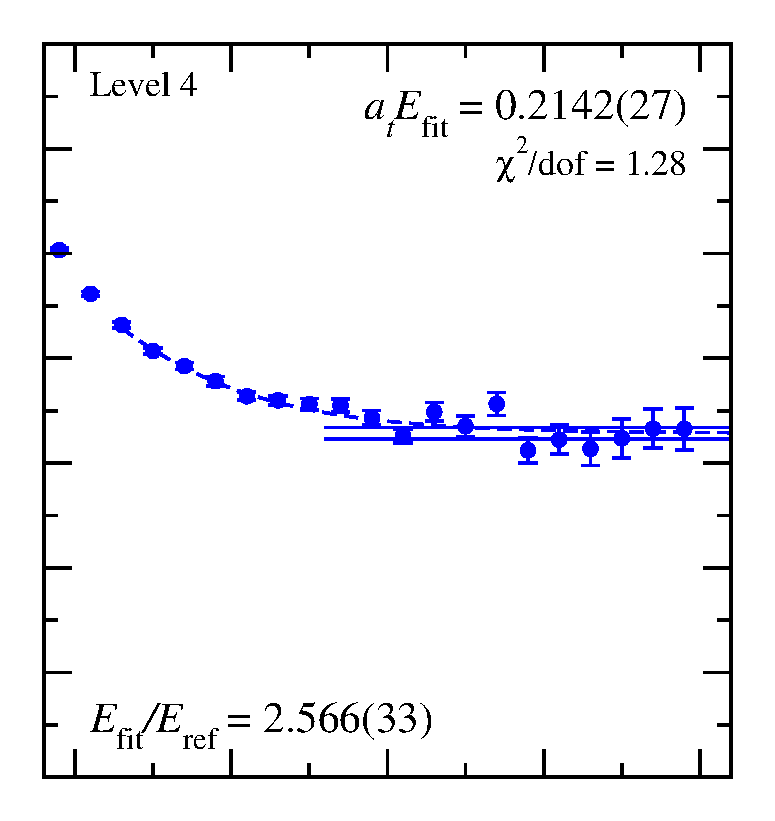
\includegraphics[width=0.28\textwidth]{figures/spectrum_a1g/no_tq/fits/fit_4.pdf}
  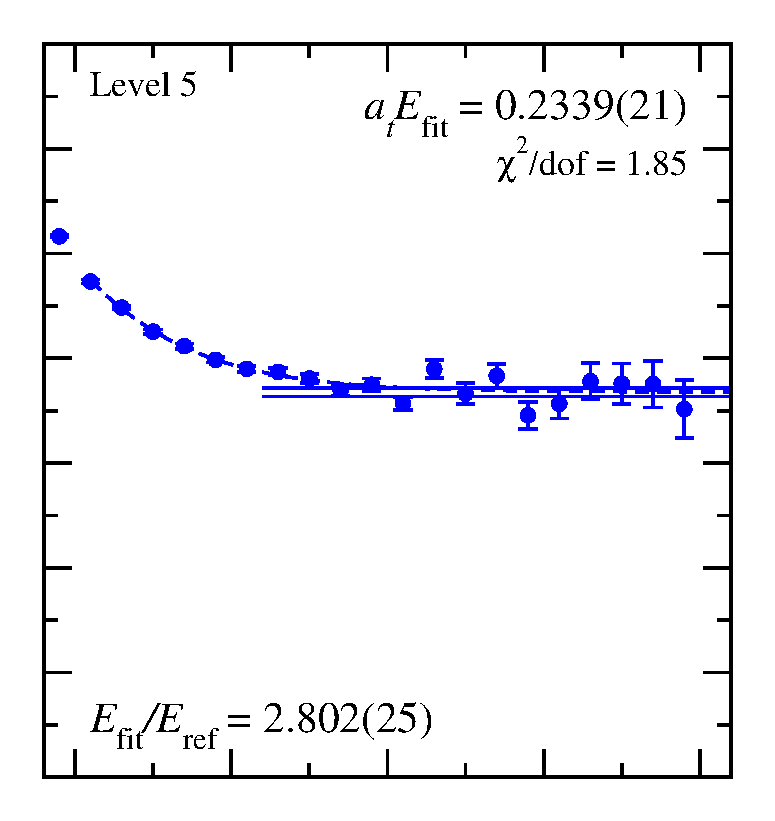
\includegraphics[width=0.28\textwidth]{figures/spectrum_a1g/no_tq/fits/fit_5.pdf}\\
  \raisebox{0.2in}{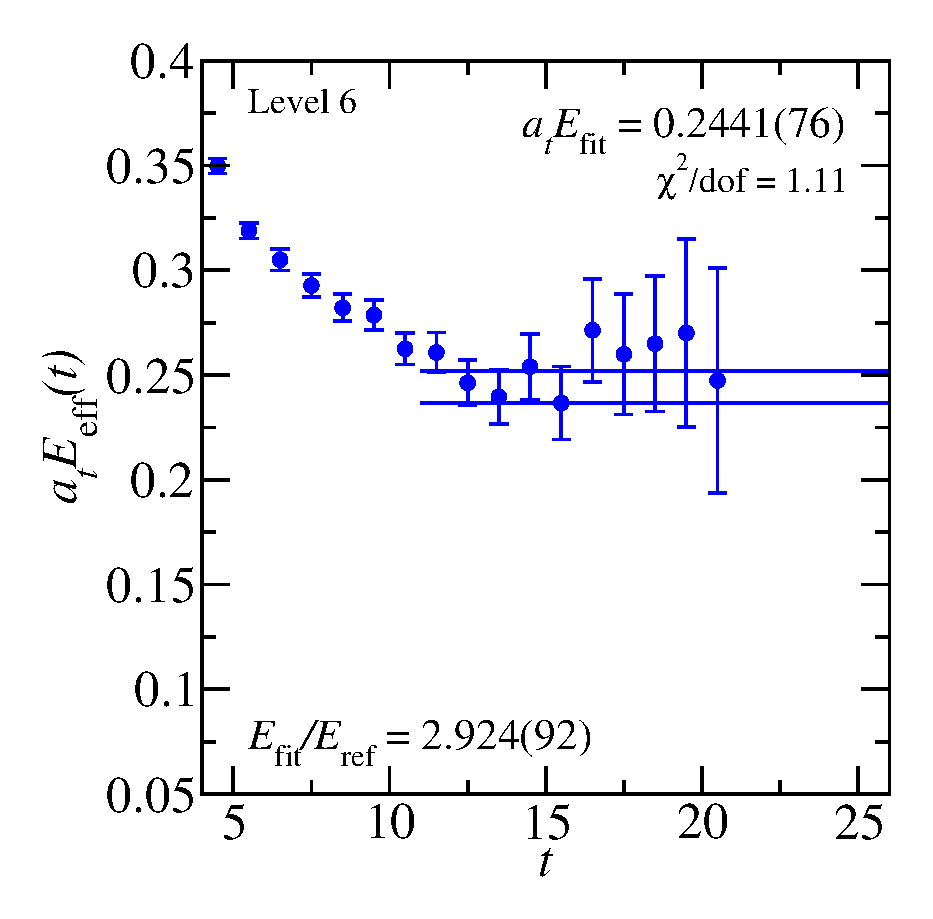
\includegraphics[width=0.336\textwidth]{figures/spectrum_a1g/no_tq/fits/fit_7.pdf}}
  \raisebox{0.2in}{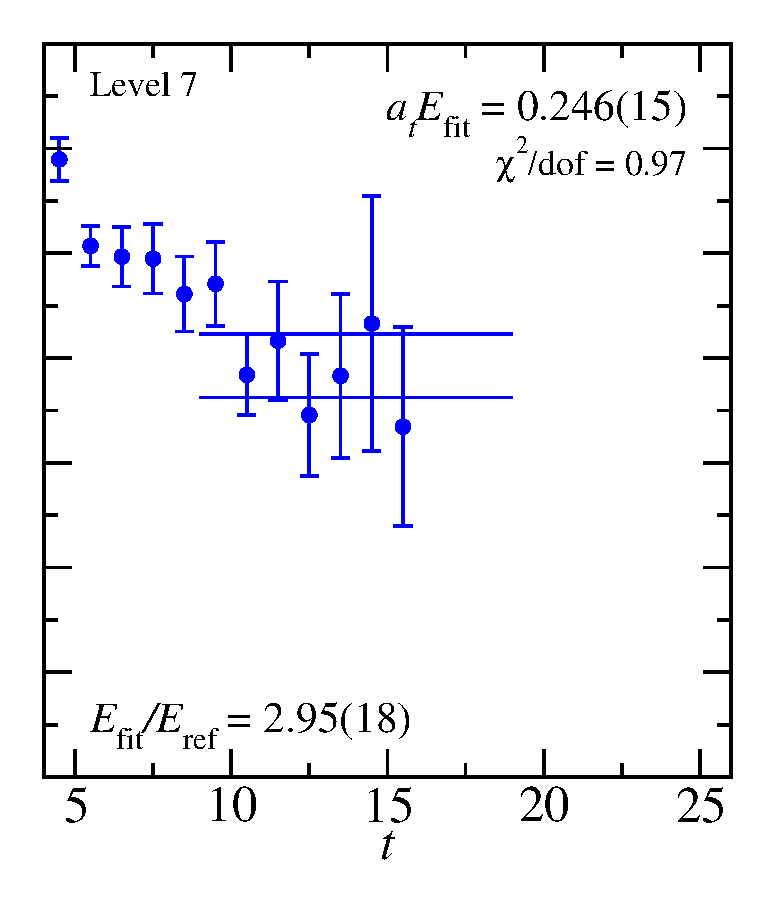
\includegraphics[width=0.28\textwidth]{figures/spectrum_a1g/no_tq/fits/fit_6.pdf}}
  \raisebox{0.2in}{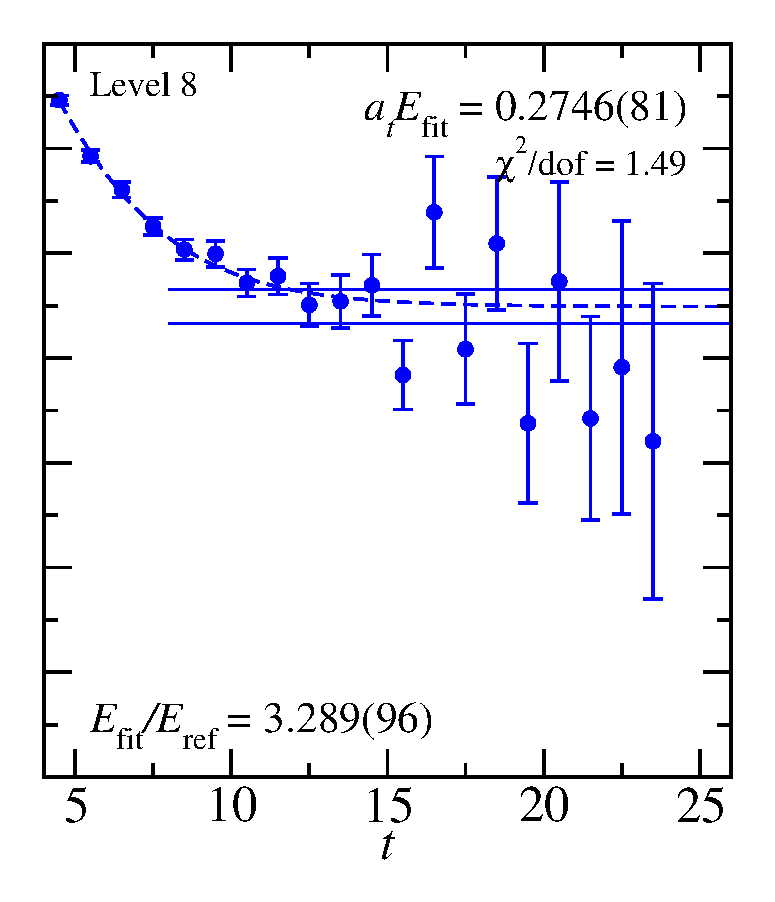
\includegraphics[width=0.28\textwidth]{figures/spectrum_a1g/no_tq/fits/fit_8.pdf}}
  \caption{Effective energies for the rotated $11\times 11$ correlator matrix in the $\kappa$ channel, using an operator basis containing no tetraquark operators. Effective energy curves calculated from correlator fits are overlaid, and fit results are shown.}
  \label{fig:kappa_no_tq_grid}
\end{figure}

\begin{figure}
  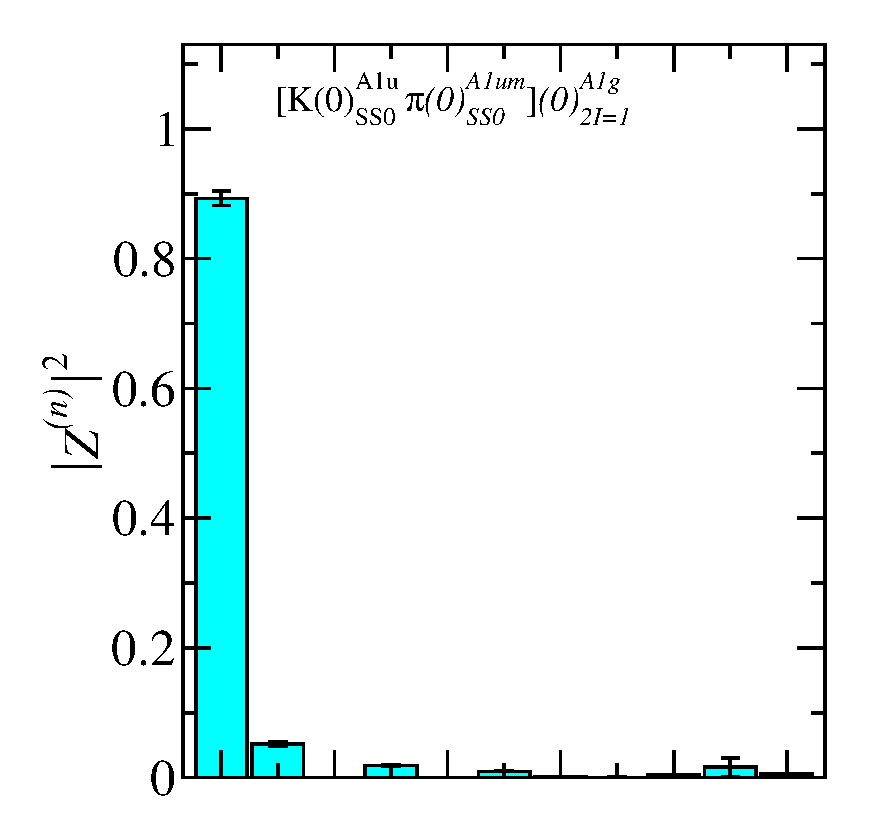
\includegraphics[width=0.304\textwidth]{figures/spectrum_a1g/no_tq/zfactors/zfactor_isodoublet_kaon_pion-A1g_1-P000-A1u-SS_0-P000-A1um-SS_0.pdf}
  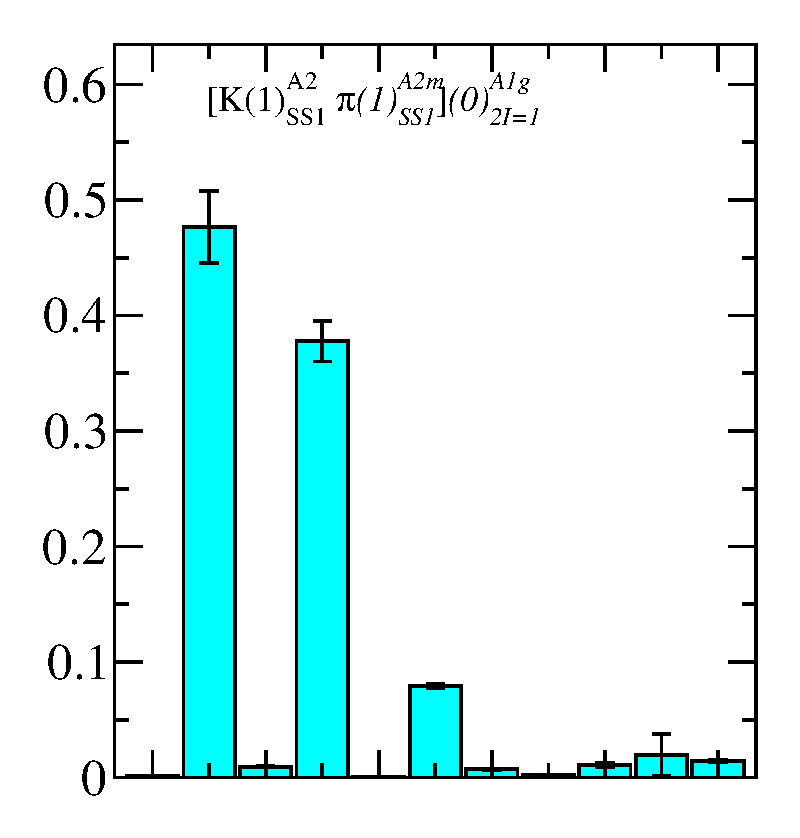
\includegraphics[width=0.28\textwidth]{figures/spectrum_a1g/no_tq/zfactors/zfactor_isodoublet_kaon_pion-A1g_1-P001-A2-SS_1-P00-1-A2m-SS_1.pdf}
  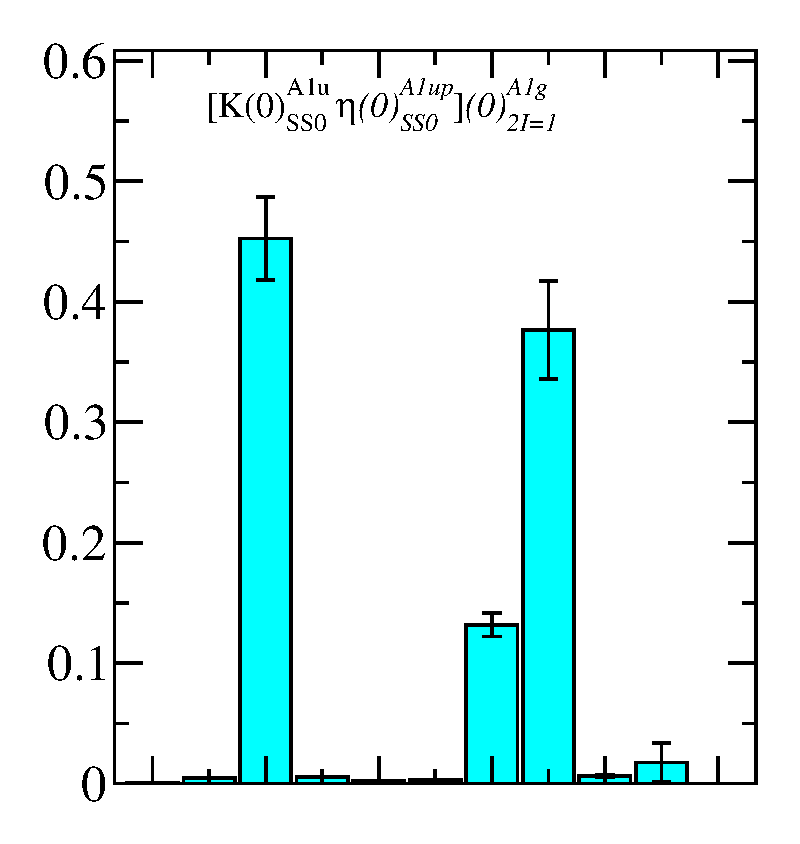
\includegraphics[width=0.28\textwidth]{figures/spectrum_a1g/no_tq/zfactors/zfactor_isodoublet_kaon_eta-A1g_1-P000-A1u-SS_0-P000-A1up-SS_0.pdf}\\
  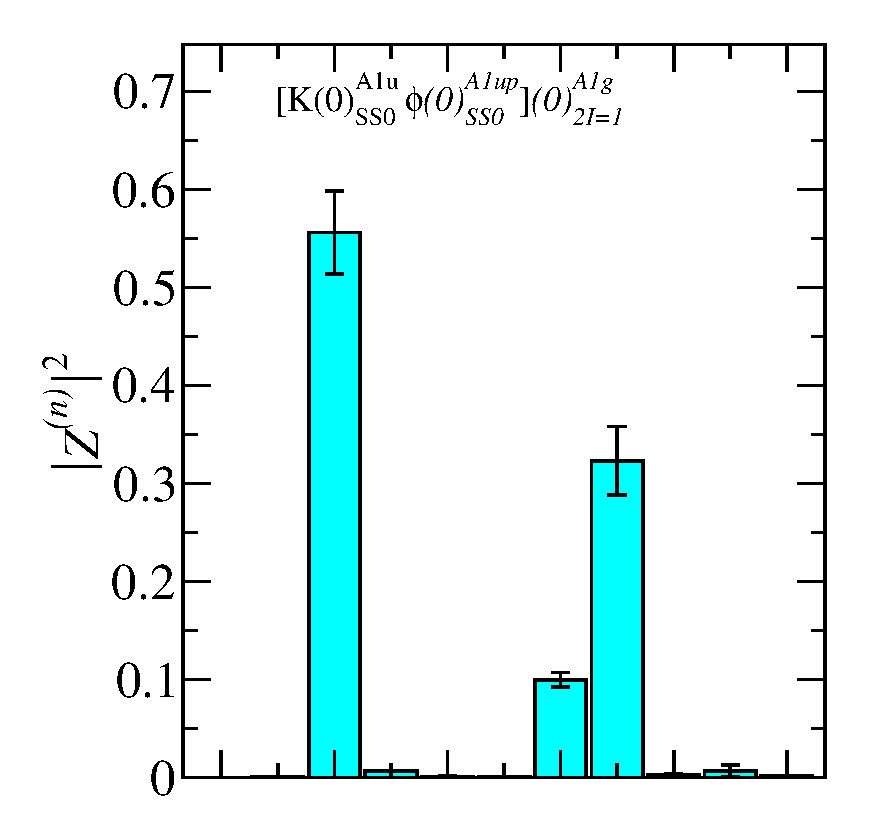
\includegraphics[width=0.304\textwidth]{figures/spectrum_a1g/no_tq/zfactors/zfactor_isodoublet_kaon_phi-A1g_1-P000-A1u-SS_0-P000-A1up-SS_0.pdf}
  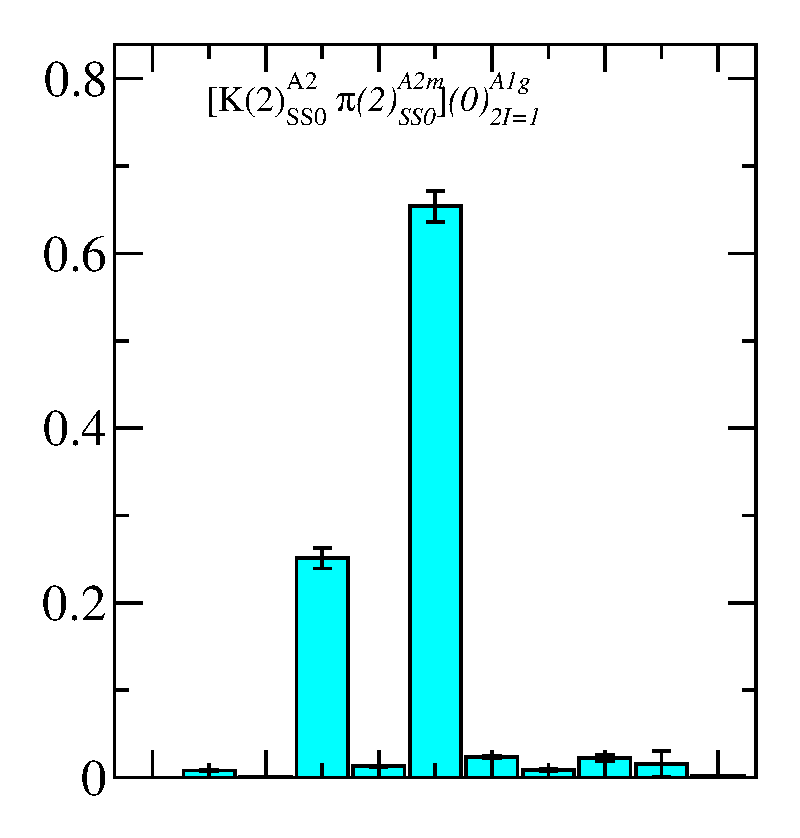
\includegraphics[width=0.28\textwidth]{figures/spectrum_a1g/no_tq/zfactors/zfactor_isodoublet_kaon_pion-A1g_1-P011-A2-SS_0-P0-1-1-A2m-SS_0.pdf}
  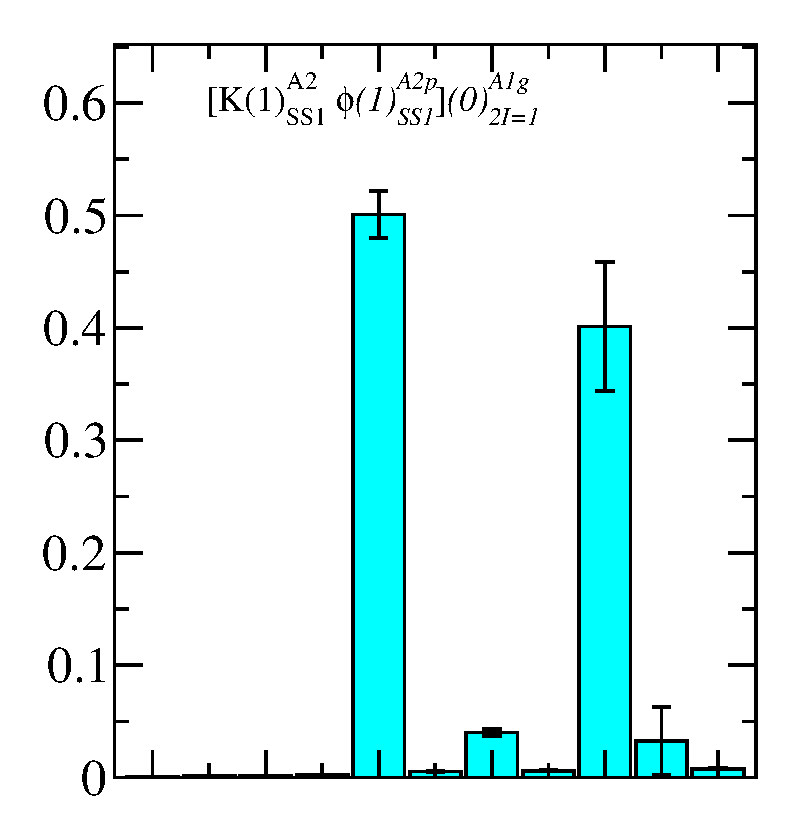
\includegraphics[width=0.28\textwidth]{figures/spectrum_a1g/no_tq/zfactors/zfactor_isodoublet_kaon_phi-A1g_1-P001-A2-SS_1-P00-1-A2p-SS_1.pdf}\\
  \raisebox{0.15in}{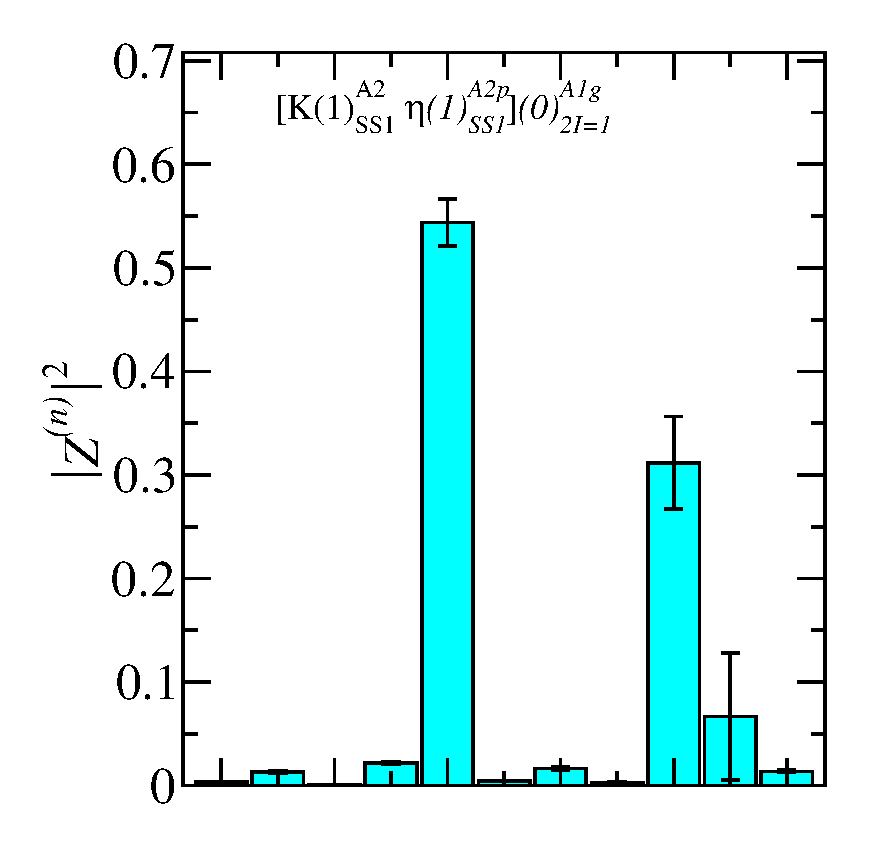
\includegraphics[width=0.304\textwidth]{figures/spectrum_a1g/no_tq/zfactors/zfactor_isodoublet_kaon_eta-A1g_1-P001-A2-SS_1-P00-1-A2p-SS_1.pdf}}
  \raisebox{0.15in}{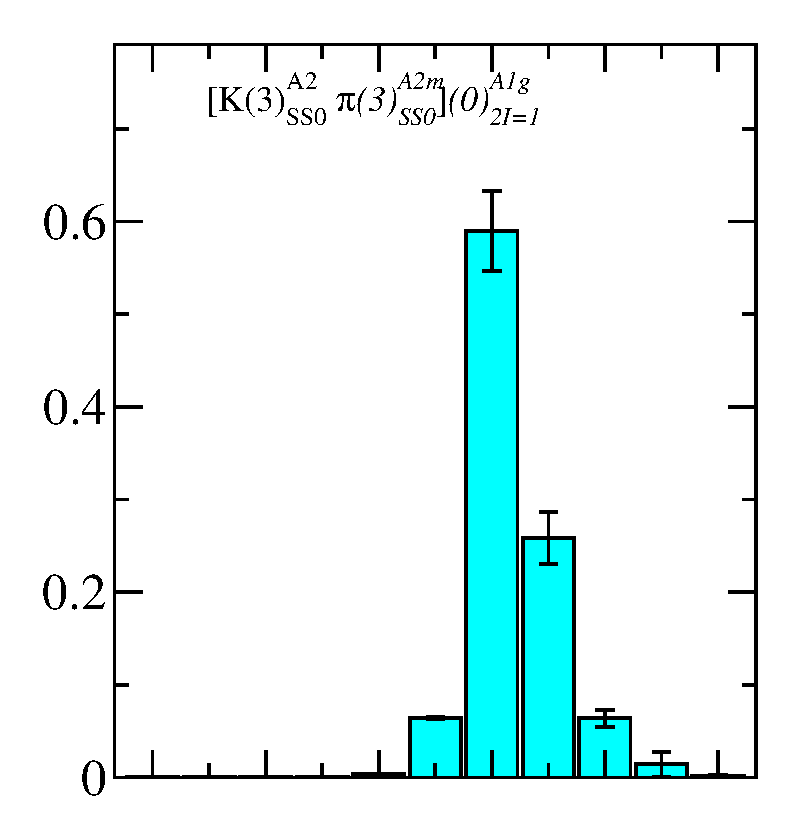
\includegraphics[width=0.28\textwidth]{figures/spectrum_a1g/no_tq/zfactors/zfactor_isodoublet_kaon_pion-A1g_1-P111-A2-SS_0-P-1-1-1-A2m-SS_0.pdf}}
  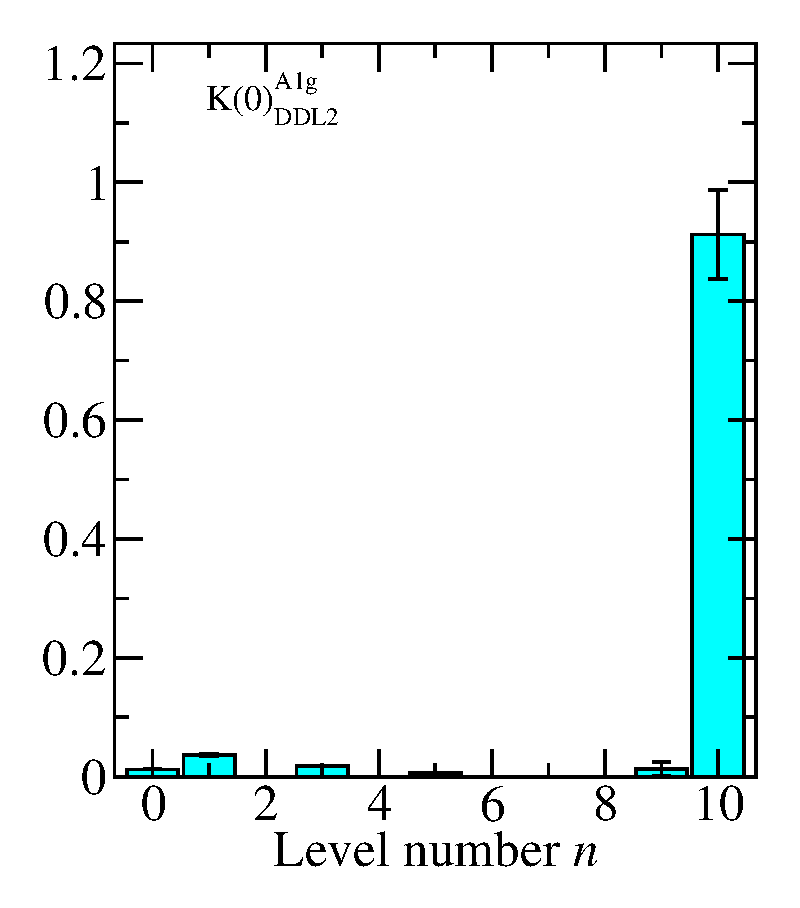
\includegraphics[width=0.28\textwidth]{figures/spectrum_a1g/no_tq/zfactors/zfactor_kaon-P000-A1g_1-DDL_2.pdf}\\
  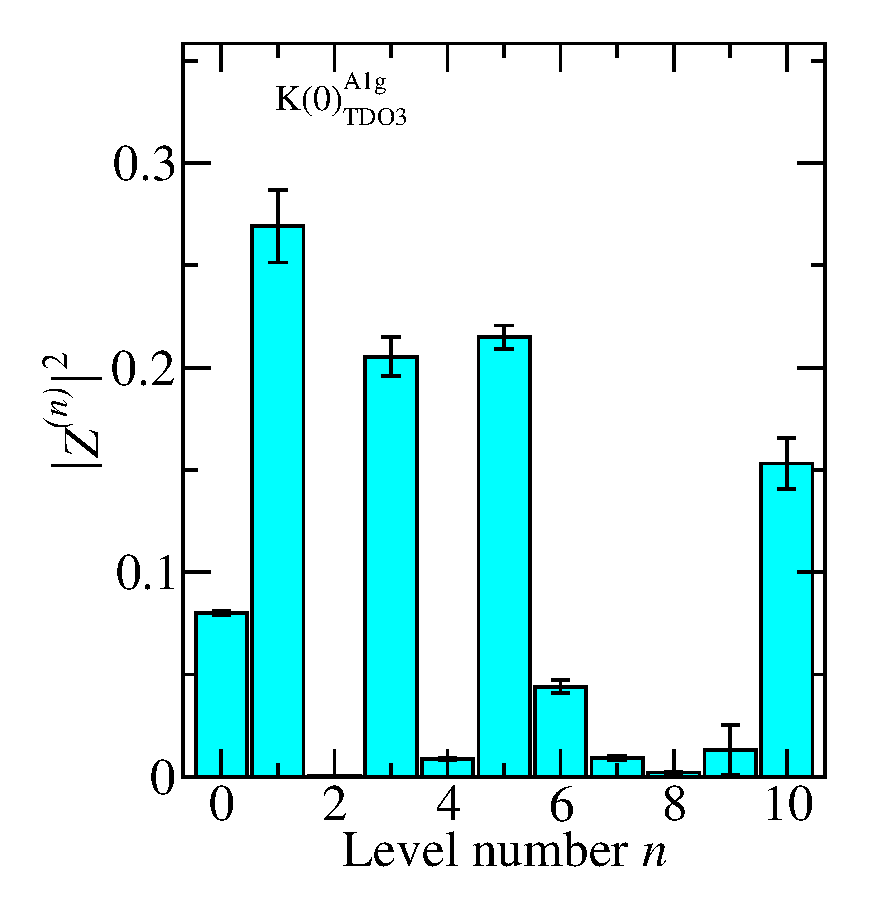
\includegraphics[width=0.304\textwidth]{figures/spectrum_a1g/no_tq/zfactors/zfactor_kaon-P000-A1g_1-TDO_3.pdf}
  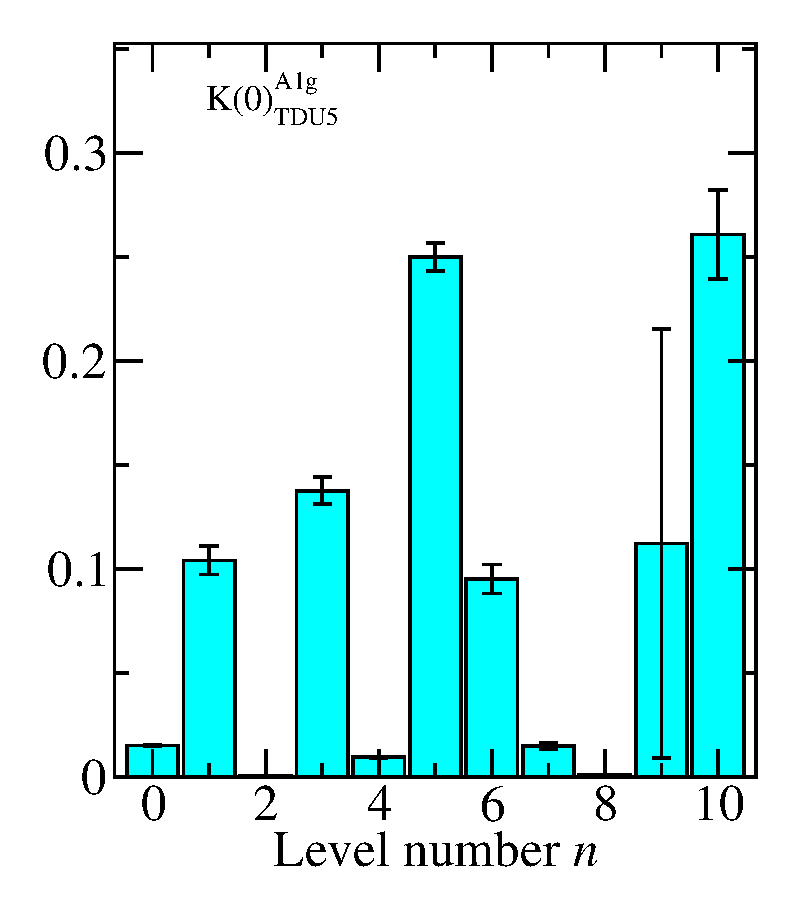
\includegraphics[width=0.28\textwidth]{figures/spectrum_a1g/no_tq/zfactors/zfactor_kaon-P000-A1g_1-TDU_5.pdf}
  \caption{Overlap factors for the rotated $11\times 11$ correlator matrix in the $\kappa$ channel, using an operator basis containing no tetraquark operators.}
  \label{fig:kappa_no_tq_zfactors}
\end{figure}

\begin{table}
  \centering
  \begin{tabular}{c|c|c|c|c}
    $E / E_K$ & $a_t E$ & Fit model & $(t_{\mathrm{min}}, {t_\mathrm{max}})$ & $\chi^2 / \rm{d.o.f.}$\\
    \hline
    1.4684(64)&0.12259(53)&2{-}exp&$(7, 26)$&0.58\\
1.908(33)&0.1593(27)&2{-}exp&$(8, 26)$&1.79\\%
2.051(74)&0.1712(62)&2{-}exp&$(4, 26)$&1.21\\
2.353(32)&0.1965(26)&2{-}exp&$(7, 26)$&1.24\\
2.566(33)&0.2142(27)&2{-}exp&$(5, 26)$&1.28\\
2.802(25)&0.2339(21)&2{-}exp&$(4, 26)$&1.85\\
2.924(92)&0.2441(76)&1{-}exp&$(11, 26)$&1.11\\
2.95(18)&0.246(15)&1{-}exp&$(9, 19)$&0.97\\
3.289(96)&0.2746(81)&2{-}exp&$(3, 26)$&1.49
  \end{tabular}
  \caption{Fit details for the spectrum obtained in the $\kappa$ channel using the operator basis given in Table~\ref{table:kappa_ops_no_tq}, which contains no tetraquark operators.}
  \label{table:kappa_no_tq_spectrum}
\end{table}

\begin{figure}
  \raisebox{-.08cm}{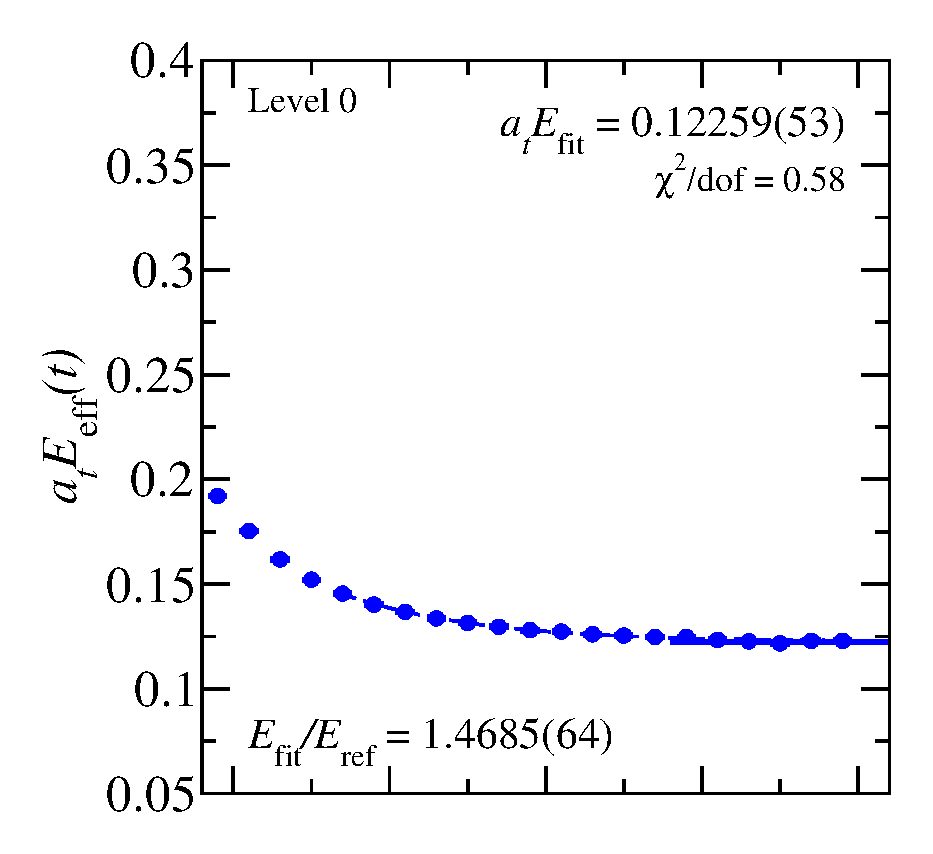
\includegraphics[width=0.336\textwidth]{figures/spectrum_a1g/with_tq/fits/fit_0.pdf}}
  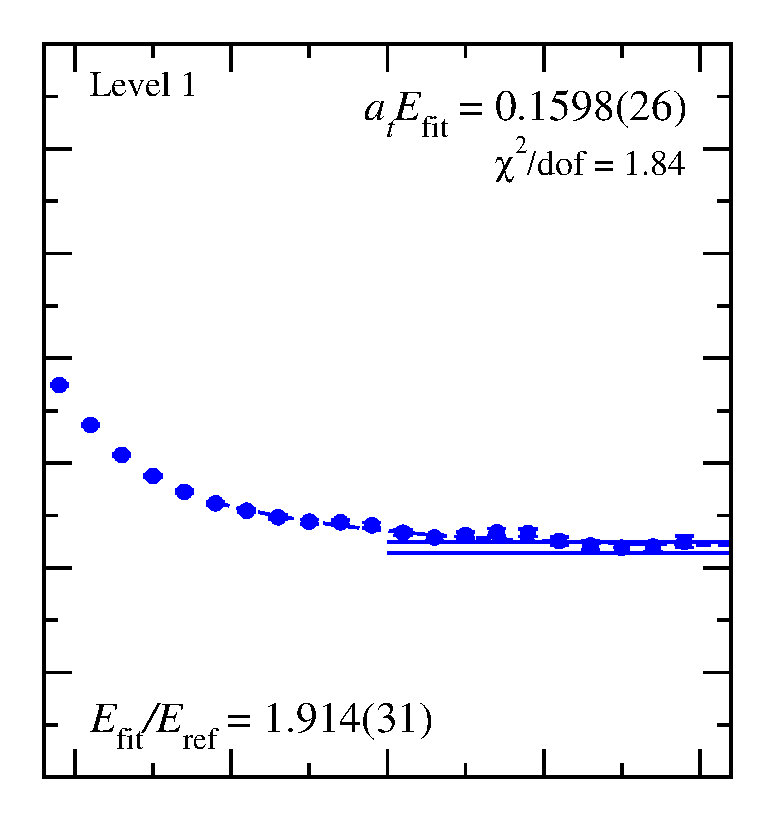
\includegraphics[width=0.28\textwidth]{figures/spectrum_a1g/with_tq/fits/fit_1.pdf}
  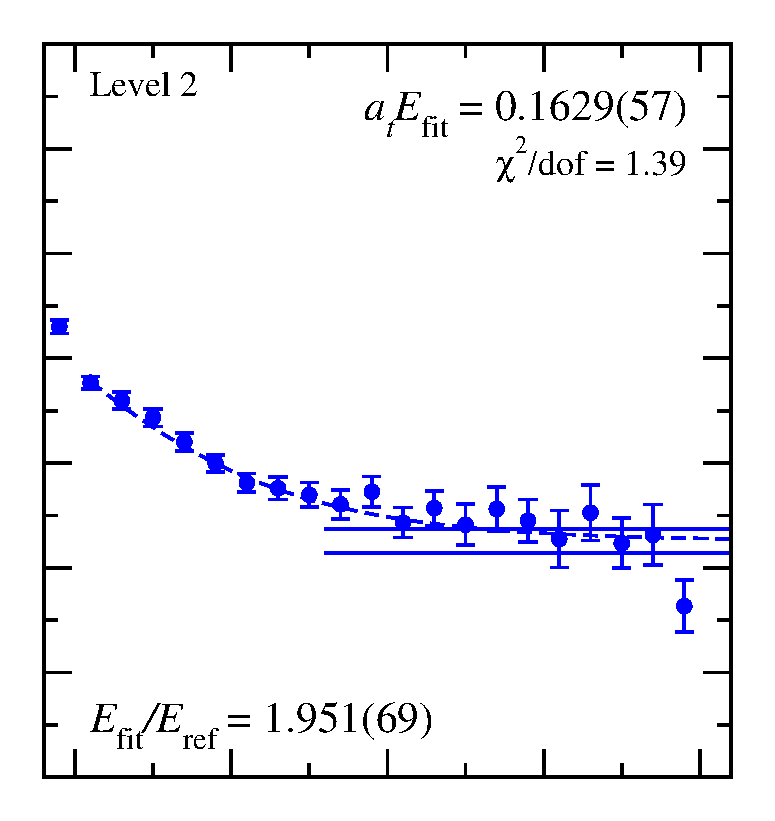
\includegraphics[width=0.28\textwidth]{figures/spectrum_a1g/with_tq/fits/fit_2.pdf}\\
  \raisebox{-.08cm}{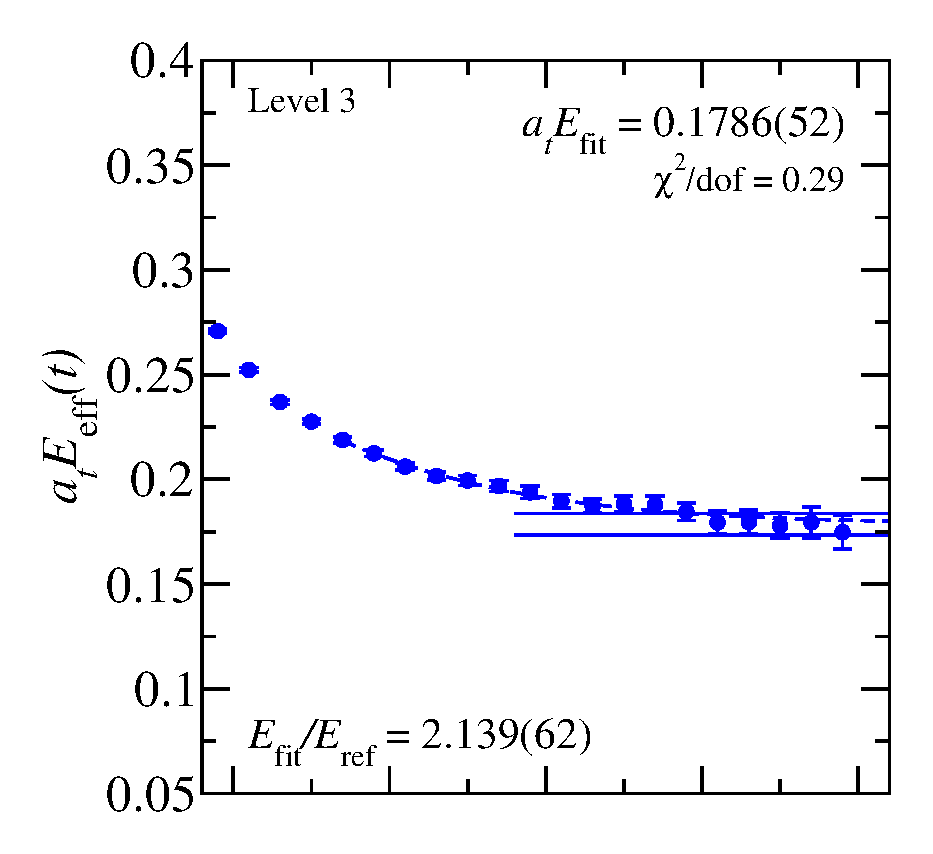
\includegraphics[width=0.336\textwidth]{figures/spectrum_a1g/with_tq/fits/fit_3.pdf}}
  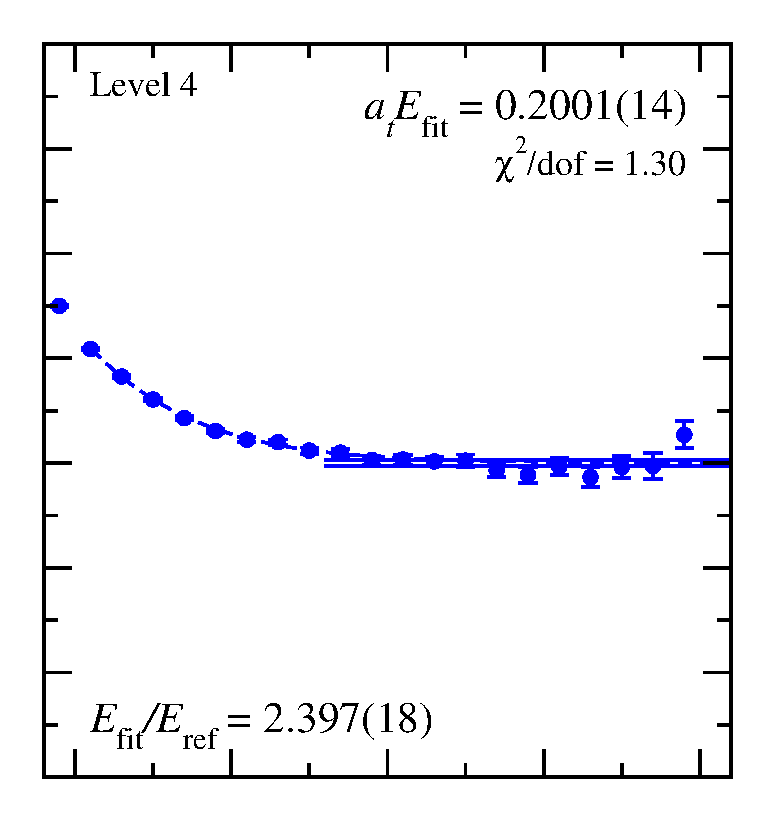
\includegraphics[width=0.28\textwidth]{figures/spectrum_a1g/with_tq/fits/fit_4.pdf}
  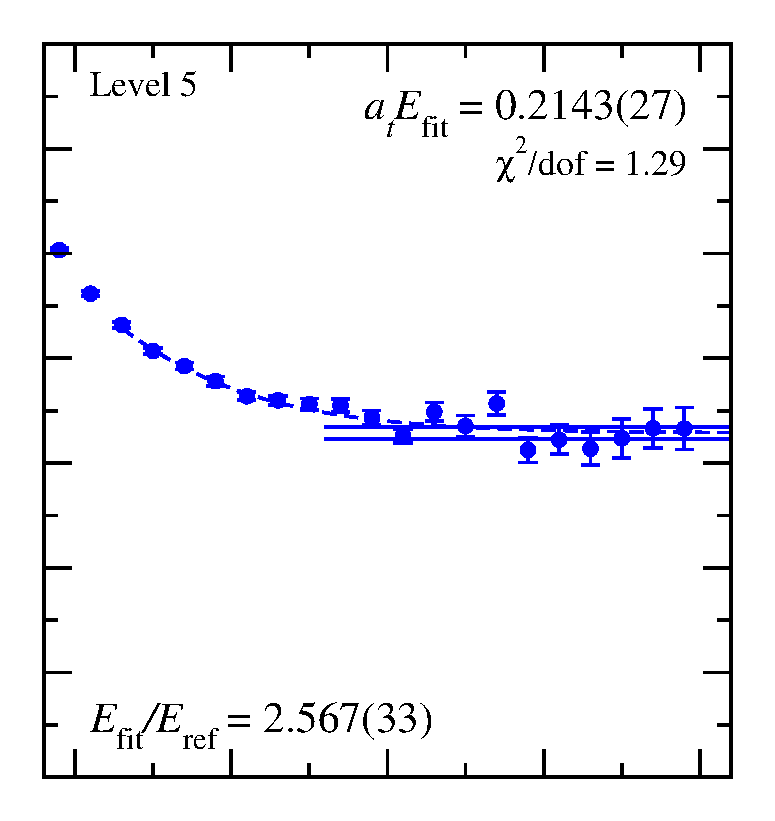
\includegraphics[width=0.28\textwidth]{figures/spectrum_a1g/with_tq/fits/fit_5.pdf}\\
  \raisebox{0.15in}{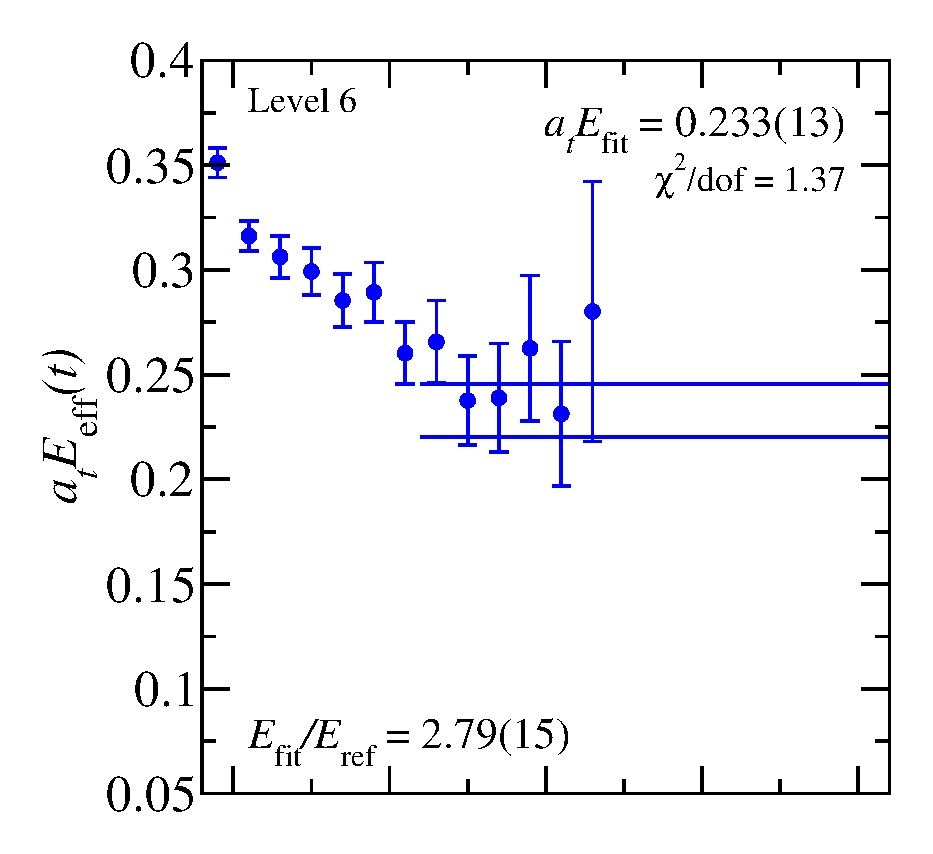
\includegraphics[width=0.338\textwidth]{figures/spectrum_a1g/with_tq/fits/fit_8.pdf}}
  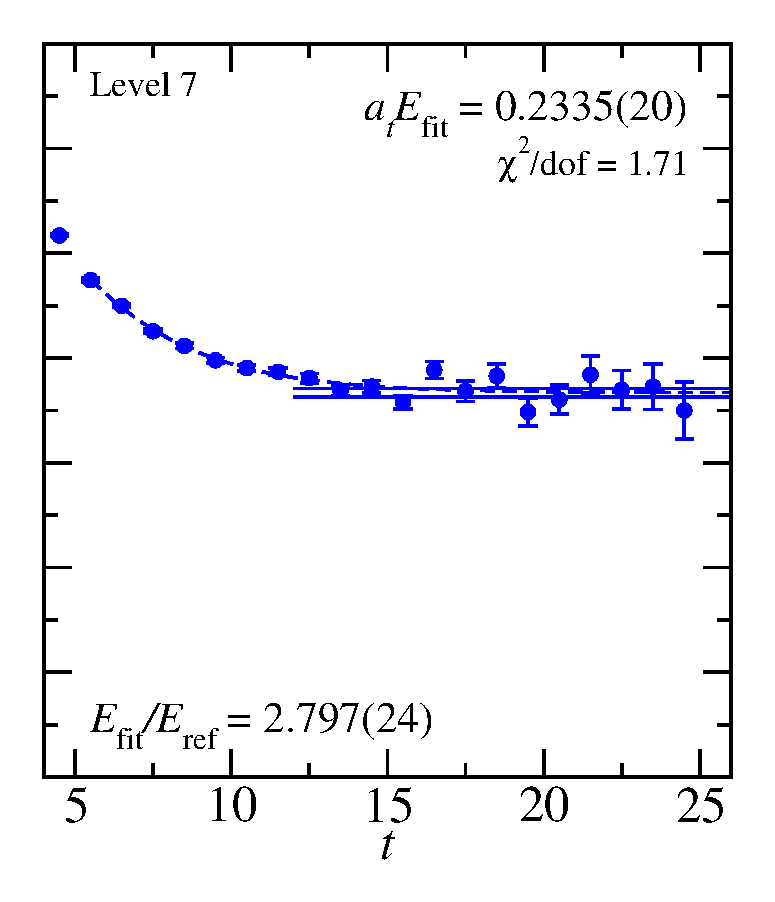
\includegraphics[width=0.28\textwidth]{figures/spectrum_a1g/with_tq/fits/fit_6.pdf}
  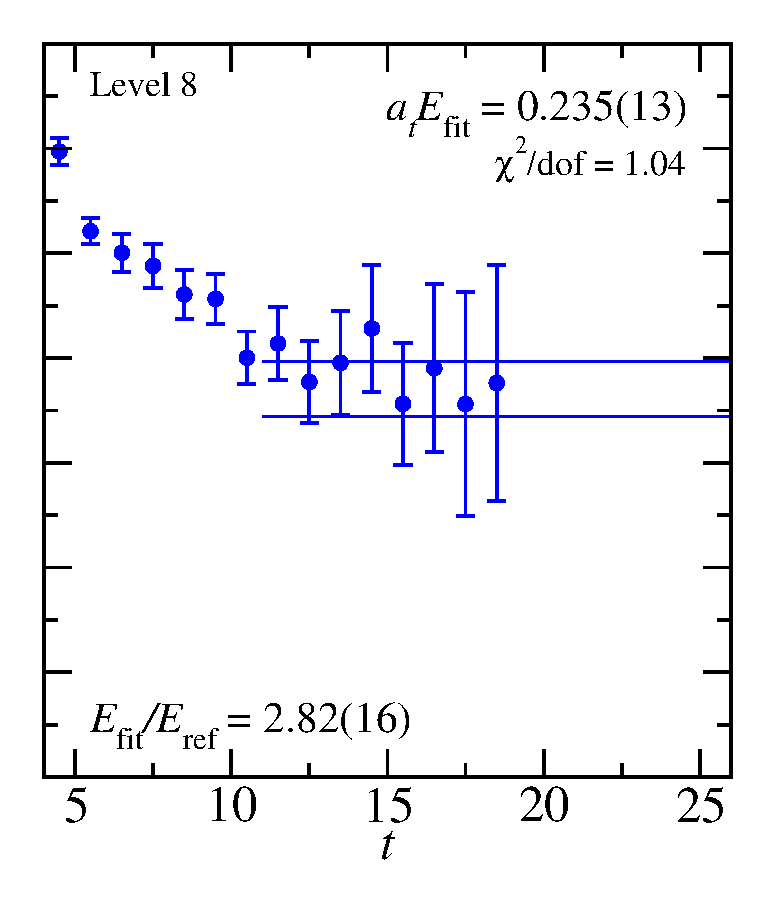
\includegraphics[width=0.28\textwidth]{figures/spectrum_a1g/with_tq/fits/fit_7.pdf}\\[-0.4cm]
  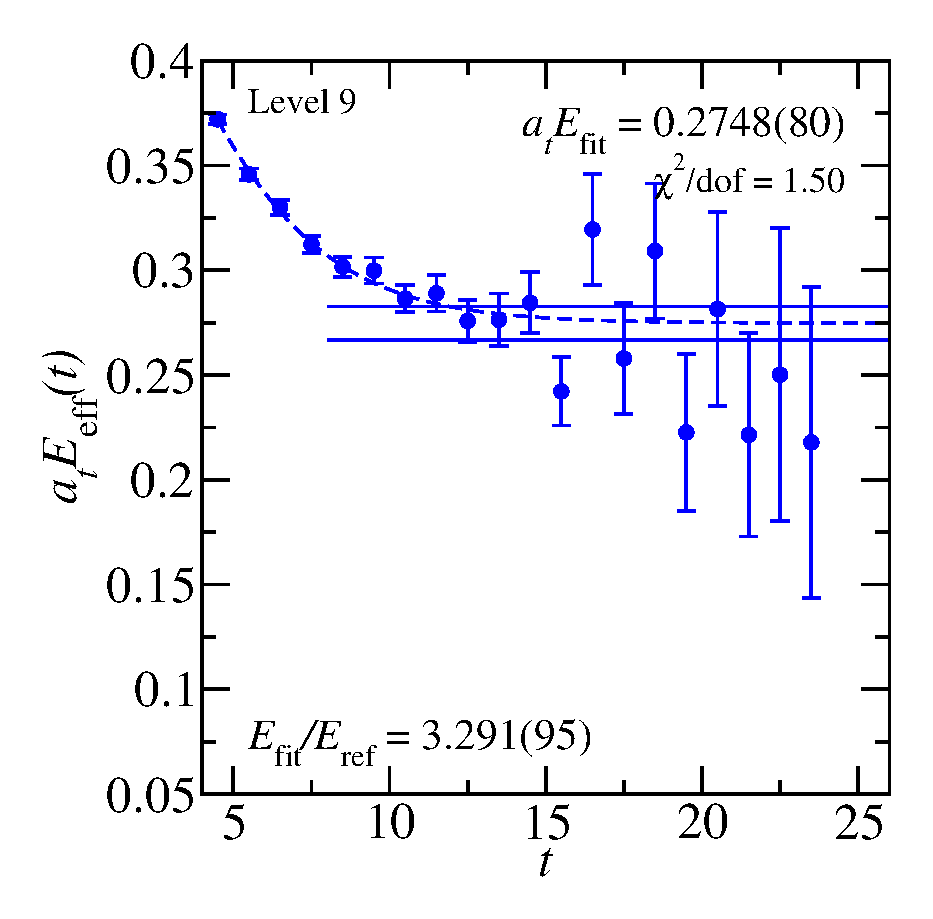
\includegraphics[width=0.336\textwidth]{figures/spectrum_a1g/with_tq/fits/fit_9.pdf}
  \caption{Effective energies for the rotated $12\times 12$ correlator matrix in the $\kappa$ channel, using the same operator basis but with the addition of one tetraquark operator. Effective energy curves calculated from correlator fits are overlaid, and fit results are shown.}
  \label{fig:kappa_with_tq_grid}
\end{figure}

\begin{figure}
  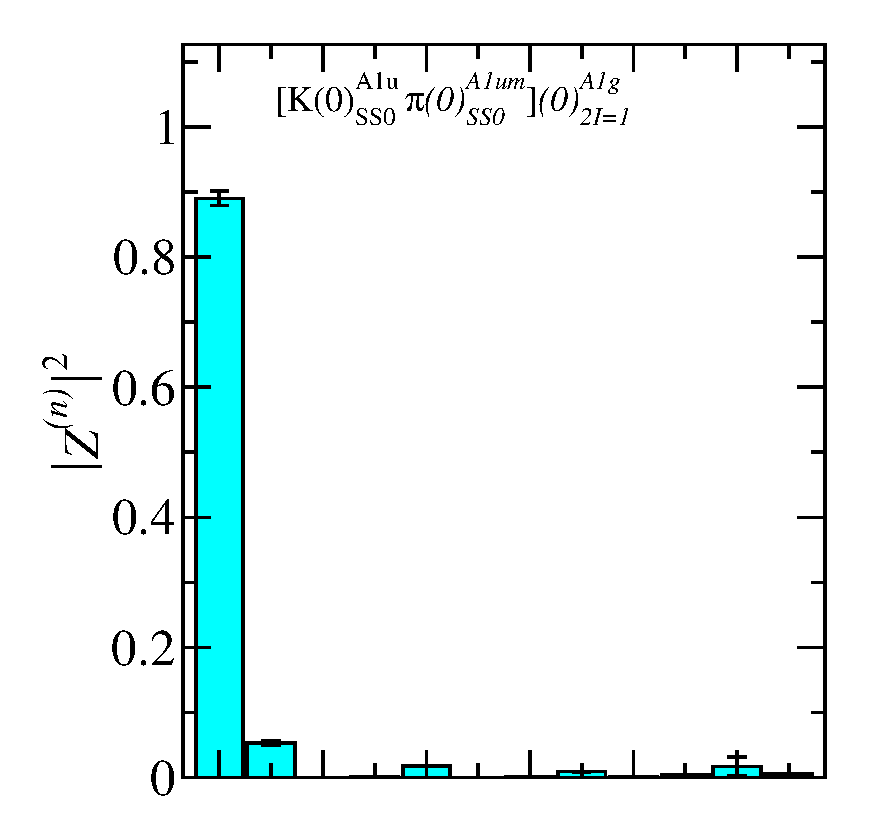
\includegraphics[width=0.304\textwidth]{figures/spectrum_a1g/with_tq/zfactors/zfactor_isodoublet_kaon_pion-A1g_1-P000-A1u-SS_0-P000-A1um-SS_0.pdf}
  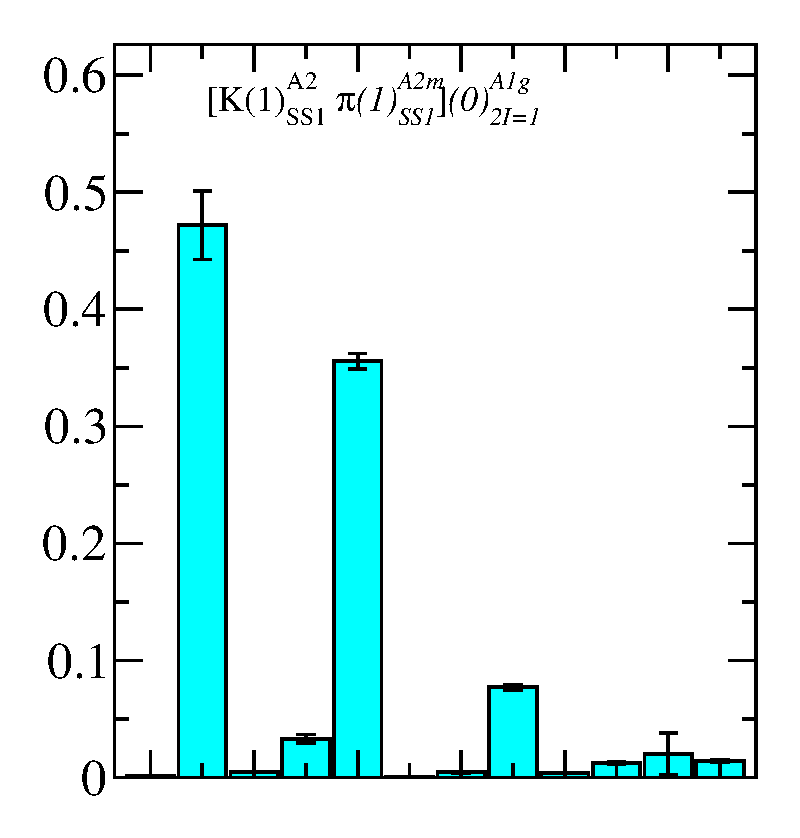
\includegraphics[width=0.28\textwidth]{figures/spectrum_a1g/with_tq/zfactors/zfactor_isodoublet_kaon_pion-A1g_1-P001-A2-SS_1-P00-1-A2m-SS_1.pdf}
  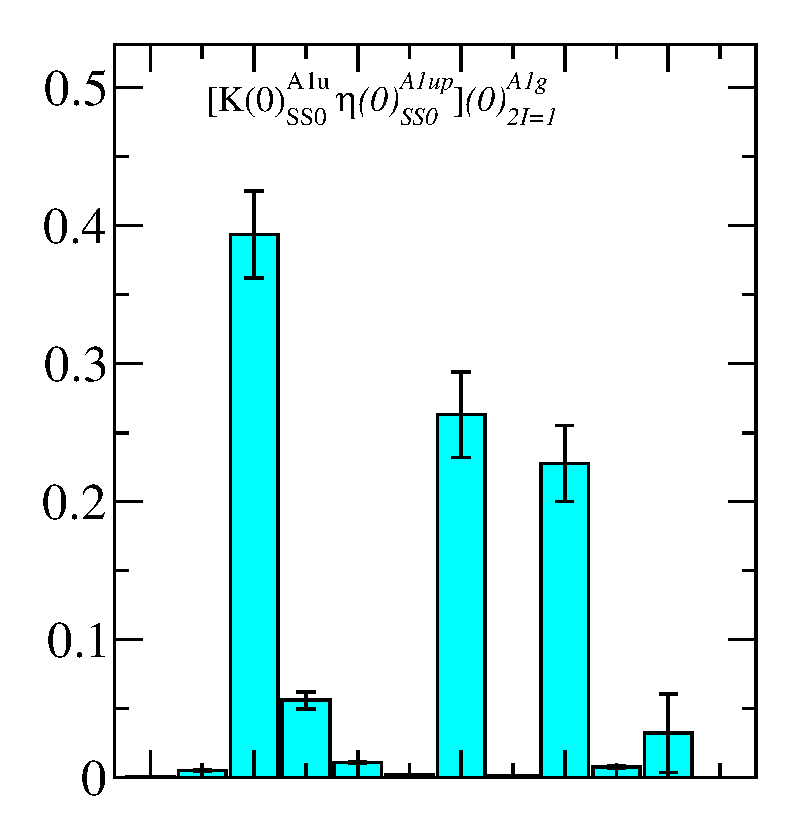
\includegraphics[width=0.28\textwidth]{figures/spectrum_a1g/with_tq/zfactors/zfactor_isodoublet_kaon_eta-A1g_1-P000-A1u-SS_0-P000-A1up-SS_0.pdf}\\
  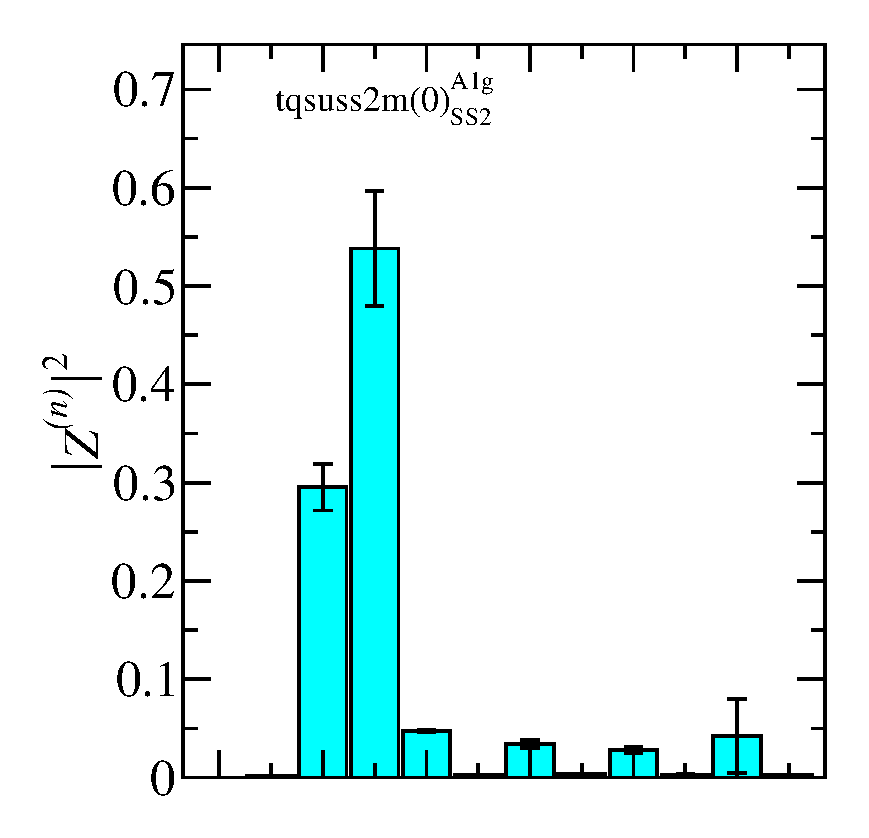
\includegraphics[width=0.304\textwidth]{figures/spectrum_a1g/with_tq/zfactors/zfactor_tqsuss2m-P000-A1g_1-SS_2.pdf}
  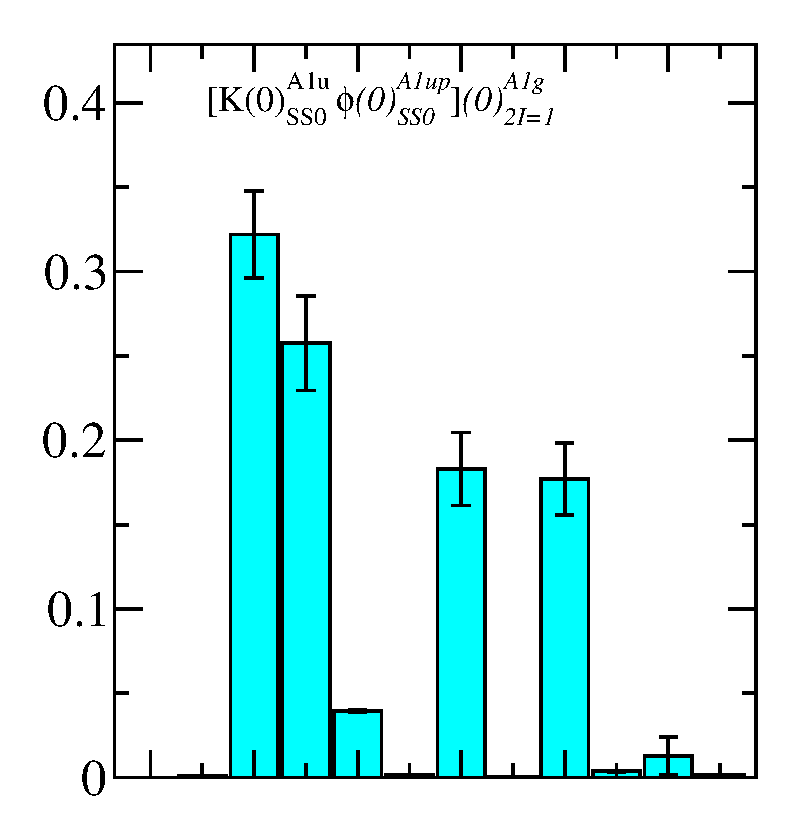
\includegraphics[width=0.28\textwidth]{figures/spectrum_a1g/with_tq/zfactors/zfactor_isodoublet_kaon_phi-A1g_1-P000-A1u-SS_0-P000-A1up-SS_0.pdf}
  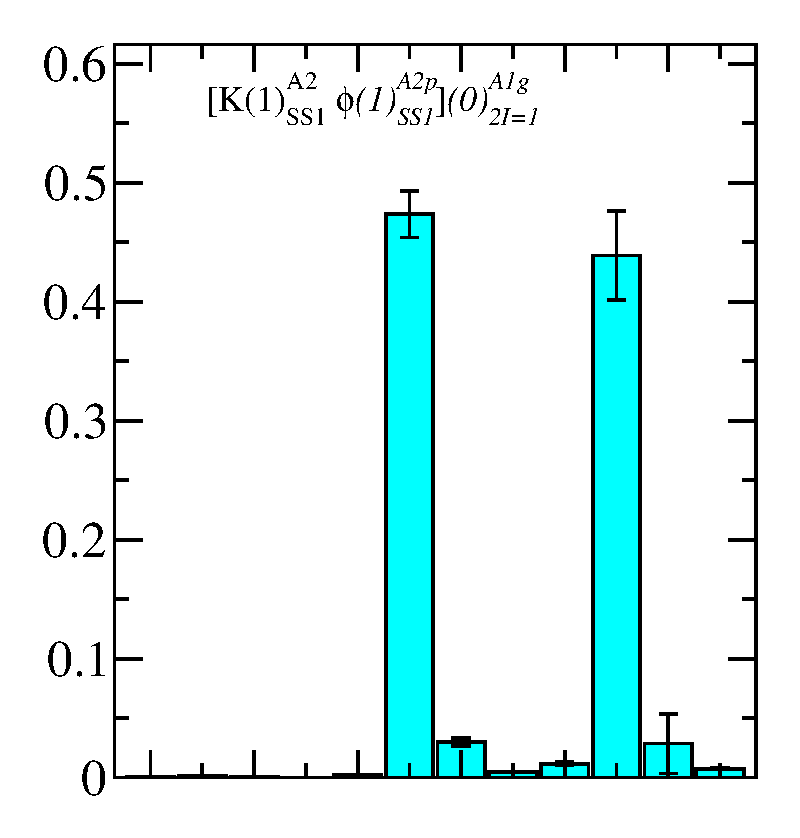
\includegraphics[width=0.28\textwidth]{figures/spectrum_a1g/with_tq/zfactors/zfactor_isodoublet_kaon_phi-A1g_1-P001-A2-SS_1-P00-1-A2p-SS_1.pdf}\\
  \includegraphics[width=0.304\textwidth]{figures/spectrum_a1g/with_tq/zfactors/zfactor_isodoublet_kaon_pion-A1g_1-P011-A2-SS_0-P0-1-1-A2m-SS_0.pdf}
  \includegraphics[width=0.28\textwidth]{figures/spectrum_a1g/with_tq/zfactors/zfactor_isodoublet_kaon_eta-A1g_1-P001-A2-SS_1-P00-1-A2p-SS_1.pdf}
  \includegraphics[width=0.28\textwidth]{figures/spectrum_a1g/with_tq/zfactors/zfactor_isodoublet_kaon_pion-A1g_1-P111-A2-SS_0-P-1-1-1-A2m-SS_0.pdf}\\
  \includegraphics[width=0.304\textwidth]{figures/spectrum_a1g/with_tq/zfactors/zfactor_kaon-P000-A1g_1-DDL_2.pdf}
  \includegraphics[width=0.28\textwidth]{figures/spectrum_a1g/with_tq/zfactors/zfactor_kaon-P000-A1g_1-TDO_3.pdf}
  \includegraphics[width=0.28\textwidth]{figures/spectrum_a1g/with_tq/zfactors/zfactor_kaon-P000-A1g_1-TDU_5.pdf}
  \caption{Overlap factors for the rotated $12\times 12$ correlator matrix in the $\kappa$ channel, using the same operator basis but with the addition of one tetraquark operator.}
  \label{fig:kappa_with_tq_zfactors}
\end{figure}

\begin{table}
  \centering
  \begin{tabular}{c|c|c|c|c}
    $E / E_K$ & $a_t E$ & Fit model & $(t_{\mathrm{min}}, {t_\mathrm{max}})$ & $\chi^2 / \rm{d.o.f.}$\\
    \hline
    1.4685(64)&0.12259(53)&2{-}exp&$(7, 26)$&0.58\\
    1.914(31)&0.1598(26)&2{-}exp&$(8, 26)$&1.84\\
    1.951(69)&0.1629(57)&2{-}exp&$(4, 26)$&1.39\\
    2.139(62)&0.1786(52)&2{-}exp&$(7, 26)$&0.29\\
    2.397(18)&0.2001(14)&2{-}exp&$(4, 26)$&1.3\\
    2.567(33)&0.2143(27)&2{-}exp&$(5, 26)$&1.29\\
    2.79(15)&0.233(13)&1{-}exp&$(11, 26)$&1.37\\
    2.797(24)&0.2335(20)&2{-}exp&$(4, 26)$&1.71\\
    2.82(16)&0.235(13)&1{-}exp&$(11, 26)$&1.04\\
    3.291(95)&0.2748(80)&2{-}exp&$(3, 26)$&1.5
  \end{tabular}
  \caption{Fit details for the spectrum obtained in the $\kappa$ channel using the same operator basis but with the addition of one tetraquark operator.}
  \label{table:kappa_with_tq_spectrum}
\end{table}

\section{$a_0(980)$ Channel}\label{sec:a0}
\subsection{Operator Bases}
The quantum numbers associated with the $a_0(980)$ are $I^G(J^{PC}) = 1^-(0^{++})$ and $S = 0$, which means that on the lattice we work in the isotriplet, nonstrange, $A_{1g}^-$ symmetry sector (see Table~\ref{table:O_occurrence_nums}). Below a cutoff of approximately 1.5 times the mass of the nucleon, near where the $a_0(1450)$ appears, we expect to see two single-hadron states (the $a_0(980)$ and the $a_0(1450)$) and several multi-hadron states. The operator basis we use, not including any tetraquark operators, is shown in Table~\ref{table:a0_ops_no_tq}. We include two single-hadron operators (one triply-displaced and one singly-displaced) in hopes of capturing states corresponding to the $a_0(980)$ and the $a_0(1450)$. We attempted to include a single-site single-hadron operator, but doing so did not produce an operator set that was sufficiently linearly-independent and produced an effective mass that was indicative of a spurious state that was leaking to the ground state. This dramatically affected the spectrum and caused it to be unstable under changes in the diagonalization time. Therefore, the single-site operator was discarded. As will be the case in Ch.~\ref{ch:sigmas}, we make use of so-called \emph{variationally improved} single-hadron operators. We obtain these operators by first diagonalizing in the subspace of single-hadron operators to form linear combinations which overlap more independently onto the single-hadron states of interest, in order to aid in level identification.

Our final class of tetraquark operators used in this channel were single-site $\overline u u \overline d u$, with both the symmetric and antisymmetric color structures included. The final tetraquark operator chosen was a $\overline u u \overline d u$, symmetric, single-site operator, which we denote as \verb+tquudu3p SS2+. Of the tetraquark operators that produced an additional level, we chose this one due to its high signal quality.
\begin{table}
  \centering
  \begin{tabular}{l|l}
    \textbf{Single-Hadron Operators} & \textbf{Two-Hadron Operators}\\
    \hline
    $\pi^{\rm{TDO}3}_{A_{1g}^-}$ & $K(0)^{\rm{SS}0}_{A_{1u}}\; \overline K(0)^{\rm{SS}0}_{A_{1u}}$\\
    $\pi^{\rm{SD}2}_{A_{1g}^-}$ & $K(1)^{\rm{SS}1}_{A_{2}}\; \overline K(1)^{\rm{SS}1}_{A_{2}}$ \\
    & $K(2)^{\rm{SS}0}_{A_{2}}\; \overline K(2)^{\rm{SS}0}_{A_{2}}$ \\
    & $K(2)^{\rm{SS}1}_{A_{2}}\; \overline K(2)^{\rm{SS}1}_{A_{2}}$ \\
    & $\eta(0)^{\rm{SS}0}_{A_{1u}^+}\; \pi(0)^{\rm{SS}0}_{A_{1u}^-}$ \\
    & $\phi(0)^{\rm{SS}0}_{A_{1u}^+}\; \pi(0)^{\rm{SS}0}_{A_{1u}^-}$ \\
    & $\eta(1)^{\rm{SS}0}_{A_{2}^+}\; \pi(1)^{\rm{SS}0}_{A_{2}^-}$ \\
    & $\phi(1)^{\rm{SS}1}_{A_{2}^+}\; \pi(1)^{\rm{SS}1}_{A_{2}^-}$ \\
    & $\eta(2)^{\rm{SS}1}_{A_{2}^+}\; \pi(2)^{\rm{SS}1}_{A_{2}^-}$ \\
    & $\phi(2)^{\rm{SS}0}_{A_{2}^+}\; \pi(2)^{\rm{SS}0}_{A_{2}^-}$ 
  \end{tabular}
  \caption{Operators used in the $a_0(980)$ channel, excluding tetraquark operators. Particle names refer to \emph{flavor content} and should not be taken literally. $K$ refers to $u\overline s$, $\overline K$ refers to $s \overline u$, $\pi$ refers to $u\overline d$, $\eta$ refers to $u\overline u + d\overline d$, and $\phi$ refers to $s\overline s$ flavor structure. The number in parentheses following the particle name denotes the square of its total momentum in lattice units, the superscript denotes displacement type, and the subscript denotes octahedral irrep and $G$-parity.}
  \label{table:a0_ops_no_tq}
\end{table}
\subsection{Spectrum Determination}
In this channel, we used a normalization time, metric time, and diagonalization time of $\tau_N=3$, $\tau_0=4$, and $\tau_d=7$, respectively. We found these parameters yielded a sufficiently diagonal correlator matrix. Fits to the diagonalized correlator set for the operator basis containing no tetraquark operators are shown in Fig.~\ref{fig:a0_no_tq_grid}, and the operator overlap factors are shown in Fig.~\ref{fig:a0_no_tq_zfactors}. Fit details are given in Table~\ref{table:a0_no_tq_spectrum}. Fits to the same operator basis, but with the addition of the $\overline u u \overline d u$ tetraquark operator, are shown in Fig.~\ref{fig:a0_with_tq_grid}, and the operator overlap factors are shown in Fig.~\ref{fig:a0_with_tq_zfactors}. Fit details are given in Table~\ref{table:a0_with_tq_spectrum}. As in the $\kappa$ channel, Fig.~\ref{fig:a0_spectrum} shows a plot of the spectrum calculated from the basis containing no tetraquark operators and the basis containing and the spectrum calculated from the basis that includes the $\overline u u \overline d u$ tetraquark operator. As in the $\kappa$ channel, we see an additional finite-volume state appear, however we see much more significant shifting of the other levels. We can attempt to explain this as follows. In the spectrum obtained in the basis with the tetraquark operator, there are two $a_0$ states onto which our \verb+ROT 0+ single-hadron operator has overlap, but our second variationally improved operator does not have overlap onto either of these states. The tetraquark operator has \emph{significant} overlap onto the lower of the two $a_0$ states, while the single-hadron operator only has minimal overlap onto it. Therefore, without the tetraquark operator present, the single-hadron operator does its best to produce both $a_0$ states, and we end up measuring a value for one mass between the two actual masses. Once we add in the tetraquark operator, we have sufficiently saturated our basis to reliably resolve both $a_0$ states. This is highly suggestive that the $a_0(980)$ does indeed have significant tetraquark content. As with the $\kappa$ channel, firm evidence for tetraquark content of the $a_0(980)$ resonance in infinite-volume will have to wait for future scattering studies.
\begin{figure}
  \centering
  \hspace*{-0.5in}\includegraphics[width=\textwidth]{figures/spectrum_a1gm/staircase.pdf}
  \caption{On the left: a spectrum obtained in the $a_0(980)$ channel using the operator basis given in Table~\ref{table:a0_ops_no_tq}, which contains no tetraquark operators. In the middle: a spectrum obtained in the $a_0(980)$ channel using the same basis but with the addition of one tetraquark operator. On the right: two-particle non-interacting energies calculated from the rest-frame masses of the constituent particles, up to the point at which we have confidently saturated the basis with two-particle operators. The horizontal dash line indicates the four-particle $\pi\pi\pi\eta$ threshold. The color of a level indicates flavor content, determined by finding which operator has the largest overlap factor with that level. If the level has significant overlap with more than one operator (with the smaller overlap being $\geq 70\%$ of the larger overlap), then a hatched box is used to denote significant mixing.}
  \label{fig:a0_spectrum}
\end{figure}

\begin{figure}
  \raisebox{0cm}{\includegraphics[width=0.329\textwidth]{figures/spectrum_a1gm/no_tq/fits/fit_0.pdf}}
  \includegraphics[width=0.28\textwidth]{figures/spectrum_a1gm/no_tq/fits/fit_1.pdf}
  \includegraphics[width=0.28\textwidth]{figures/spectrum_a1gm/no_tq/fits/fit_2.pdf}\\
  \raisebox{-0.0in}{\includegraphics[width=0.329\textwidth]{figures/spectrum_a1gm/no_tq/fits/fit_3.pdf}}
  \includegraphics[width=0.28\textwidth]{figures/spectrum_a1gm/no_tq/fits/fit_5.pdf}
  \includegraphics[width=0.28\textwidth]{figures/spectrum_a1gm/no_tq/fits/fit_4.pdf}\\
  \raisebox{-0.00in}{\includegraphics[width=0.329\textwidth]{figures/spectrum_a1gm/no_tq/fits/fit_6.pdf}}
  \includegraphics[width=0.28\textwidth]{figures/spectrum_a1gm/no_tq/fits/fit_7.pdf}
  \includegraphics[width=0.28\textwidth]{figures/spectrum_a1gm/no_tq/fits/fit_8.pdf}\\
  \caption{Effective energies for the rotated $12\times 12$ correlator matrix in the $a_0(980)$ channel, using an operator basis containing no tetraquark operators. Effective energy curves calculated from correlator fits are overlaid, and fit results are shown. For all effective mass plots in this work, a time step of $\Delta t = 3$ is used for the discretized derivative.}
  \label{fig:a0_no_tq_grid}
\end{figure}

\begin{figure}
  \includegraphics[width=0.304\textwidth]{figures/spectrum_a1gm/no_tq/zfactors/zfactor_isotriplet-S0-P000-A1gm_1-ROT-0.pdf}
  \includegraphics[width=0.28\textwidth]{figures/spectrum_a1gm/no_tq/zfactors/zfactor_isotriplet-S0-P000-A1gm_1-ROT-1.pdf}
  \includegraphics[width=0.28\textwidth]{figures/spectrum_a1gm/no_tq/zfactors/zfactor_isotriplet_phi_pion-A1gm_1-P000-A1up-SS_0-P000-A1um-SS_0.pdf}\\
  \includegraphics[width=0.304\textwidth]{figures/spectrum_a1gm/no_tq/zfactors/zfactor_isotriplet_eta_pion-A1gm_1-P000-A1up-SS_0-P000-A1um-SS_0.pdf}
  \includegraphics[width=0.28\textwidth]{figures/spectrum_a1gm/no_tq/zfactors/zfactor_isotriplet_kaon_kbar-A1gm_1-P000-A1u-SS_0-P000-A1u-SS_0.pdf}
  \includegraphics[width=0.28\textwidth]{figures/spectrum_a1gm/no_tq/zfactors/zfactor_isotriplet_phi_pion-A1gm_1-P001-A2p-SS_1-P00-1-A2m-SS_1.pdf}\\
  \includegraphics[width=0.304\textwidth]{figures/spectrum_a1gm/no_tq/zfactors/zfactor_isotriplet_kaon_kbar-A1gm_1-P001-A2-SS_1-P00-1-A2-SS_1.pdf}
  \includegraphics[width=0.28\textwidth]{figures/spectrum_a1gm/no_tq/zfactors/zfactor_isotriplet_phi_pion-A1gm_1-P011-A2p-SS_0-P0-1-1-A2m-SS_0.pdf}
  \includegraphics[width=0.28\textwidth]{figures/spectrum_a1gm/no_tq/zfactors/zfactor_isotriplet_eta_pion-A1gm_1-P001-A2p-SS_0-P00-1-A2m-SS_0.pdf}\\
  \includegraphics[width=0.304\textwidth]{figures/spectrum_a1gm/no_tq/zfactors/zfactor_isotriplet_eta_pion-A1gm_1-P011-A2p-SS_1-P0-1-1-A2m-SS_1.pdf}
  \includegraphics[width=0.28\textwidth]{figures/spectrum_a1gm/no_tq/zfactors/zfactor_isotriplet_kaon_kbar-A1gm_1-P011-A2-SS_0-P0-1-1-A2-SS_0.pdf}
  \includegraphics[width=0.28\textwidth]{figures/spectrum_a1gm/no_tq/zfactors/zfactor_isotriplet_kaon_kbar-A1gm_1-P011-A2-SS_1-P0-1-1-A2-SS_1.pdf}
  \cprotect\caption{Overlap factors for the rotated $12\times 12$ correlator matrix in the $a_0(980)$ channel, using an operator basis containing no tetraquark operators. Operators labeled by \verb+ROT N+ denote our variationally improved single-hadron operators.}
  \label{fig:a0_no_tq_zfactors}
\end{figure}

\begin{table}
  \centering
  \begin{tabular}{c|c|c|c|c}
    $E / E_K$ & $a_t E$ & Fit model & $(t_{\mathrm{min}}, {t_\mathrm{max}})$ & $\chi^2 / \rm{d.o.f.}$\\
    \hline
    1.475(74)&0.1231(62)&2{-}exp&$(3, 26)$&1.13\\
    2.034(25)&0.1698(21)&2{-}exp&$(5, 26)$&1.3\\
    2.19(17)&0.183(14)&1{-}exp&$(9, 26)$&0.99\\
    2.224(35)&0.1857(29)&2{-}exp&$(6, 26)$&1.08\\
    2.30(15)&0.192(13)&2{-}exp&$(6, 26)$&0.81\\
    2.452(33)&0.2047(27)&2{-}exp&$(6, 26)$&0.45\\
    2.828(45)&0.2361(37)&2{-}exp&$(6, 26)$&0.71\\
    2.971(32)&0.2480(26)&2{-}exp&$(4, 26)$&1.66\\
    5.00(39)&0.417(33)&1{-}exp&$(8, 18)$&1.23
  \end{tabular}
  \caption{Fit details for the spectrum obtained in the $a_0(980)$ channel using the operator basis given in Table~\ref{table:a0_ops_no_tq}, which contains no tetraquark operators.}
  \label{table:a0_no_tq_spectrum}
\end{table}

\begin{figure}
  \includegraphics[width=0.329\textwidth]{figures/spectrum_a1gm/with_tq/fits/fit_0.pdf}
  \includegraphics[width=0.28\textwidth]{figures/spectrum_a1gm/with_tq/fits/fit_2.pdf}
  \includegraphics[width=0.28\textwidth]{figures/spectrum_a1gm/with_tq/fits/fit_1.pdf}\\
  \includegraphics[width=0.329\textwidth]{figures/spectrum_a1gm/with_tq/fits/fit_3.pdf}
  \includegraphics[width=0.28\textwidth]{figures/spectrum_a1gm/with_tq/fits/fit_4.pdf}
  \includegraphics[width=0.28\textwidth]{figures/spectrum_a1gm/with_tq/fits/fit_5.pdf}\\
  \raisebox{0.48cm}{\includegraphics[width=0.329\textwidth]{figures/spectrum_a1gm/with_tq/fits/fit_6.pdf}}
  \includegraphics[width=0.28\textwidth]{figures/spectrum_a1gm/with_tq/fits/fit_7.pdf}
  \includegraphics[width=0.28\textwidth]{figures/spectrum_a1gm/with_tq/fits/fit_8.pdf}\\[-0.4cm]
  \includegraphics[width=0.329\textwidth]{figures/spectrum_a1gm/with_tq/fits/fit_9.pdf}
  \caption{Effective energies for the rotated $13\times 13$ correlator matrix in the $a_0(980)$ channel, using the same operator basis but with the addition of one tetraquark operator. Effective energy curves calculated from correlator fits are overlaid, and fit results are shown.}
  \label{fig:a0_with_tq_grid}
\end{figure}

\begin{figure}
  \includegraphics[width=0.24\textwidth]{figures/spectrum_a1gm/with_tq/zfactors/zfactor_isotriplet-S0-P000-A1gm_1-ROT-0.pdf}
  \includegraphics[width=0.22\textwidth]{figures/spectrum_a1gm/with_tq/zfactors/zfactor_isotriplet-S0-P000-A1gm_1-ROT-1.pdf}
  \includegraphics[width=0.22\textwidth]{figures/spectrum_a1gm/with_tq/zfactors/zfactor_tquudu3p-P000-A1gm_1-SS_2.pdf}
  \includegraphics[width=0.22\textwidth]{figures/spectrum_a1gm/with_tq/zfactors/zfactor_isotriplet_phi_pion-A1gm_1-P000-A1up-SS_0-P000-A1um-SS_0.pdf}\\
  \includegraphics[width=0.24\textwidth]{figures/spectrum_a1gm/with_tq/zfactors/zfactor_isotriplet_eta_pion-A1gm_1-P000-A1up-SS_0-P000-A1um-SS_0.pdf}
  \includegraphics[width=0.22\textwidth]{figures/spectrum_a1gm/with_tq/zfactors/zfactor_isotriplet_kaon_kbar-A1gm_1-P000-A1u-SS_0-P000-A1u-SS_0.pdf}
  \includegraphics[width=0.22\textwidth]{figures/spectrum_a1gm/with_tq/zfactors/zfactor_isotriplet_phi_pion-A1gm_1-P001-A2p-SS_1-P00-1-A2m-SS_1.pdf}
  \includegraphics[width=0.22\textwidth]{figures/spectrum_a1gm/with_tq/zfactors/zfactor_isotriplet_kaon_kbar-A1gm_1-P001-A2-SS_1-P00-1-A2-SS_1.pdf}\\
  \raisebox{0.12in}{\includegraphics[width=0.24\textwidth]{figures/spectrum_a1gm/with_tq/zfactors/zfactor_isotriplet_phi_pion-A1gm_1-P011-A2p-SS_0-P0-1-1-A2m-SS_0.pdf}}
  \includegraphics[width=0.22\textwidth]{figures/spectrum_a1gm/with_tq/zfactors/zfactor_isotriplet_eta_pion-A1gm_1-P001-A2p-SS_0-P00-1-A2m-SS_0.pdf}
  \includegraphics[width=0.22\textwidth]{figures/spectrum_a1gm/with_tq/zfactors/zfactor_isotriplet_eta_pion-A1gm_1-P011-A2p-SS_1-P0-1-1-A2m-SS_1.pdf}
  \includegraphics[width=0.22\textwidth]{figures/spectrum_a1gm/with_tq/zfactors/zfactor_isotriplet_kaon_kbar-A1gm_1-P011-A2-SS_0-P0-1-1-A2-SS_0.pdf}\\[-0.2cm]
  \includegraphics[width=0.24\textwidth]{figures/spectrum_a1gm/with_tq/zfactors/zfactor_isotriplet_kaon_kbar-A1gm_1-P011-A2-SS_1-P0-1-1-A2-SS_1.pdf}
  \cprotect\caption{Overlap factors for the rotated $13\times 13$ correlator matrix in the $a_0(980)$ channel, using the same operator basis given in Table~\ref{table:a0_ops_no_tq}, with the addition of one tetraquark operator. Operators labeled by \verb+ROT N+ denote our variationally improved single-hadron operators.}
  \label{fig:a0_with_tq_zfactors}
\end{figure}

\begin{table}
  \centering
  \begin{tabular}{c|c|c|c|c}
    $E / E_K$ & $a_t E$ & Fit model & $(t_{\mathrm{min}}, {t_\mathrm{max}})$ & $\chi^2 / \rm{d.o.f.}$\\
    \hline
    1.410(79)&0.1177(66)&2{-}exp&$(3, 26)$&1.12\\
    2.014(29)&0.1681(24)&2{-}exp&$(6, 26)$&1.99\\
    2.03(11)&0.1692(92)&2{-}exp&$(3, 26)$&1.03\\
    2.41(13)&0.201(11)&1{-}exp&$(9, 26)$&0.82\\
    2.537(42)&0.2118(35)&2{-}exp&$(3, 26)$&1.18\\
    2.586(26)&0.2159(21)&2{-}exp&$(4, 26)$&0.67\\
    2.84(12)&0.237(10)&2{-}exp&$(3, 24)$&0.99\\
    2.947(40)&0.2461(33)&2{-}exp&$(4, 26)$&0.9\\
    2.964(35)&0.2475(29)&2{-}exp&$(4, 26)$&1.64\\
    5.01(39)&0.418(33)&1{-}exp&$(8, 18)$&1.25
  \end{tabular}
  \caption{Fit details for the spectrum obtained in the $a_0(980)$ channel using the operator basis given in Table~\ref{table:a0_ops_no_tq}, with the addition of one tetraquark operator.}
  \label{table:a0_with_tq_spectrum}
\end{table}

\chapter{$\Sigma$ Baryon Spectroscopy}\label{ch:sigmas}
In this chapter, we present results on the finite-volume spectrum of $\Sigma$ baryons in several $I=1$, $S=-1$ symmetry sectors, namely $G_{1g}$, $G_{1u}$, $H_u$, $H_g$, $G_{2g}$, and $G_{2u}$. We have constructed correlator matrices from large bases of single- and two-hadron operators, which allows us to more accurately determine the spectrum than in previous works. We compare our results to experimentally observed $\Sigma$ resonances, and compare to a previous work using a smaller lattice, heavier pion, and no two-hadron operators.

The $\Sigma$ baryons are unstable resonances. However, lattice QCD Monte Carlo results are obtained in finite volume.  In finite volume, only the energies of the finite-volume stationary states can be determined.  To deduce the spectrum of resonances from the finite-volume energies would require a technique similar to that employed by L\"uscher~\cite{Luscher:1990ck} but extended beyond two-particle thresholds.  Such a technique does not yet exist and would be prohibitively difficult to carry out.  Our goal here is much more humble.  We wish mainly to identify the finite-volume states produced primarily by three-quark single baryon operators.  The energies of such states are expected to fall near the resonance energies of the $\Sigma$ baryons which are predominantly three-quark excitations.  The narrower the resonance, the closer our estimates should be.  In other words, our results should be viewed as a qualitative study of the resonance spectrum.  Note that resonances which are primarily ``molecular'' in nature cannot be determined in this way.  Futhermore, our use of an unphysical light quark mass to make the calculations practical will cause further deviations from experiment.

All past studies~\cite{Edwards:2012fx, Bulava:2009jb, Bulava:2010yg, Edwards:2011jj} suffer from these same flaws.  However, all past studies have only used single baryon operators.  This study is the first to also use meson-baryon operators, significantly improving the spectrum determination.
\section{Ensemble}
Ensemble details are identical to those described in Sec.~\ref{sec:ensemble}.
\section{$G_{1g}$ Spectrum}
The isotriplet, $S=-1$, $G_{1g}$ symmetry channel is parity-positive and contains spins $\frac{1}{2}$, $\frac{7}{2}$, $\frac{9}{2}$, and beyond. In this channel, we expect to see several experimentally observed states including the physical $\Sigma$, the $\Sigma(1660)$, and the $\Sigma(2030)$, which have spins $\frac{1}{2}$, $\frac{1}{2}$, and $\frac{7}{2}$, respectively. In addition to these single-hadron states, we expect to see many multi-hadron states. Reliably extracting finite-volume single-hadron states that correspond to resonances in infinite-volume requires the use of multi-hadron operators, since we expect the finite-volume counterpart to a resonance to have some overlap onto its decay products. While it would be ideal to compute many-hadron correlators, computing correlators for states with greater than two hadrons is prohibitively expensive, so we limit ourselves to using operators which are designed to create at most two hadrons.

In general, we start with a large basis of operators, and \emph{prune} out those which are either too noisy or not sufficiently linearly independent. For the single-hadron operators, we started with a large basis 16 operators, and pruned our set down to just 7. For the two-hadron operators, we started with a basis of 25 operators, and pruned our set down to just 21. The final basis of single- and two-hadron operators used to extract the spectrum in this channel is given in Table~\ref{table:g1g_ops}. Just as in Sec.~\ref{sec:a0}, we make use of variationally improved single-hadron operators. That is, we first diagonalize in the subspace of single-hadron operators to form linear combinations which overlap more independently onto the single-hadron states of interest, in order to aid in level identification. We found that a normalization time, metric time, and diagonalization time of $\tau_N=3$, $\tau_0=4$, and $\tau_d=7$ ensured that the rotated correlator matrix remained sufficiently diagonal. It is important to note that while $\eta\Sigma$ two-hadron operators are included, there is no corresponding $\phi\Sigma$ operator, so we expect to miss a two-hadron state. This will be the case in every channel in this chapter.

\begin{table}[H]
    \centering
    \begin{tabular}{l|l}
        \textbf{Single-Hadron Operators} & \textbf{Two-Hadron Operators} \\
        \hline
        $\Sigma_{G_{1g}}^{DDI0}$ & $\pi(0)_{A_{1u}^-}^{SS0}\Lambda(0)_{G_{1u}}^{SS2}$\\
        $\Sigma_{G_{1g}}^{DDI22}$ & $\pi(0)_{A_{1u}^-}^{SS0}\Lambda(0)_{G_{1u}}^{SS3}$\\
        $\Sigma_{G_{1g}}^{DDL55}$ & $\pi(1)_{A_2^-}^{SS1}\Lambda(1)_{G_1}^{SS1}$\\
        $\Sigma_{G_{1g}}^{SS2}$ & $\pi(2)_{A_2^-}^{SS0}\Lambda(2)_{G}^{SS0}$\\
        $\Sigma_{G_{1g}}^{SS3}$ & $\pi(3)_{A_2^-}^{SS0}\Lambda(3)_{G}^{SS0}$\\
        $\Sigma_{G_{1g}}^{TDT65}$ & $\pi(1)_{A_2^-}^{SS0}\Sigma(1)_{G_1}^{SS0}$\\
        $\Sigma_{G_{1g}}^{TDT72}$ & $\pi(1)_{A_2^-}^{SS1}\Sigma(1)_{G_1}^{SS0}$\\
        & $\pi(1)_{A_2^-}^{SS1}\Sigma(1)_{G_1}^{SS2}$\\
        & $\pi(2)_{A_2^-}^{SS0}\Sigma(2)_{G}^{SS1}$\\
        & $\pi(3)_{A_2^-}^{SS0}\Sigma(3)_{G}^{SS4}$\\
        & $\overline K(1)_{A_1}^{SS2}N(1)_{G_1}^{SS0}$\\
        & $\overline K(1)_{A_2}^{SS0}N(1)_{G_1}^{SS0}$\\
        & $\overline K(1)_{A_2}^{SS1}N(1)_{G_1}^{SS0}$\\
        & $\overline K(1)_{E}^{SS2}N(1)_{G_1}^{SS0}$\\
        & $\overline K(4)_{A_2}^{SS1}N(4)_{G_1}^{SS0}$\\
        & $\overline K(2)_{A_2}^{SS0}N(2)_{G}^{SS0}$\\
        & $\overline K(2)_{A_2}^{SS1}N(2)_{G}^{SS0}$\\
        & $\overline K(3)_{A_2}^{SS0}N(3)_{G}^{SS0}$\\
        & $\overline K(1)_{A_2}^{SS1}\Delta(1)_{G_1}^{SS0}$\\
        & $K(1)_{A_2}^{SS1}\Xi(1)_{G_1}^{SS0}$\\
        & $\eta(1)_{A_2^+}^{SS1}\Sigma(1)_{G_1}^{SS0}$
    \end{tabular}
    \caption{Operators used in the isotriplet $S=-1$ $G_{1g}$ symmetry sector.}\label{table:g1g_ops}
\end{table}
The spectrum obtained in terms of the kaon mass (obtained from the fit given in Ch.~\ref{ch:tetraquarks}) is shown in Fig.~\ref{fig:g1g_spectrum}. Correlator fits are shown in Fig.~\ref{fig:g1g_fits}, and fit details are given in Table~\ref{table:g1g_fits}. A qualitative attempt at level identification is made by determining, for each operator, which level overlaps maximally with the state created by that operator. Additionally, we are interested in operators which have significant but non-maximal overlaps onto a given state, which can inform us about mixing. Mixing is important since we expect a resonance to have overlap onto not only states created by single-hadron operators, but also states corresponding to potential decay products. A comparison of the experimentally observed resonances in this channel to the low-lying single-hadron-dominated states we obtain from the lattice is shown in Fig.~\ref{fig:g1g_exp}. Because we do not expect to reliably extract the masses of the highest few levels, we do not include the highest two single-hadron-dominated states in our comparison to experiment, and their energy determinations should be viewed as being much less reliable. When comparing results to experiment, we use the nucleon mass (obtained from the fit shown in Fig.~\ref{fig:nucleon_fit}) as a reference, since it is more sensitive than the kaon mass to the unphysically heavy pion. However, we are able to determine the kaon mass with better precision, so we use it as a reference in our full spectrum plots, e.g.\ Fig~\ref{fig:g1g_spectrum}. Our findings seem to agree qualitatively with previous lattice results by Edwards et al.\ in Ref.~\cite{Edwards:2012fx}, shown in Fig.~\ref{fig:edwards}, produced using a $16^3$ lattice with a pion mass of $m_\pi \approx 391$ MeV and no two-hadron operators. In Ref.~\cite{Edwards:2012fx}, they found one low-lying state, corresponding to the physical $\Sigma$, and four higher nearly-degenerate states with two less well determined levels just above the four levels. We find the same pattern: one low-lying level, with four higher well-determined nearly-degenerate levels, and two more states nearby but not well determined.

In comparing our results to experiment, we see qualitative agreement in energy: A well-determined ground state corresponding to the physical $\Sigma$ and several states above it near in energy to the $\Sigma(1660)$ and the $\Sigma(2030)$. Our results are certainly affected by our unphysically heavy pion and the fact that we are comparing infinite-volume resonances to their finite-volume stationary-state counterpart, however, so we should not expect rigorous agreement. Additionally, as will be the case in many of the other channels in this chapter, we do not find agreement between the number of single-hadron-dominated states on the lattice and the number of resonances seen in experiment in the same energy range. This should not come as a surprise, however. The problem of ``missing resonances''~\cite{Koniuk:1979vw} has long been an issue; the number of baryon resonances predicted by quark models has long disagreed with the number seen in experiment. In Ref.~\cite{Koniuk:1979vw}, Koniuk and Isgur attempt to explain this by claiming that over half of all predicted resonances are too inelastic to be easily seen.

\begin{figure}[H]
    \centering
    \hspace*{-0.5in}\includegraphics[width=\textwidth]{figures/sigmas/g1g/staircase_mk.pdf}
    \caption[The spectrum for the isotriplet $S=-1$ $G_{1g}$ channel, obtained by fitting the energies and overlap factors of the diagonalized correlator matrix.]{The spectrum for the isotriplet $S=-1$ $G_{1g}$ channel, obtained by fitting the energies and overlap factors of the diagonalized correlator matrix. A qualitative attempt at level identification is made by determining, for each operator, which level overlaps maximally with the state created by that operator. If a level does not overlap maximally with any operator's state, we denote its flavor content as ``N/A''. Because we expect a single-hadron resonance to have significant overlap with potential decay products, we also use hatching to denote any level which has an overlap of $\geq 70\%$ of the maximum overlap with a single-hadron operator. The vertical dashed line indicates the point beyond which our energy extractions are too high to be reliable.}\label{fig:g1g_spectrum}
\end{figure}

\begin{figure}[H]
    \centering
    \hspace*{-1cm}\includegraphics[width=0.8\textwidth]{figures/edwards.pdf}
    \caption[Observed single-hadron states on a $16^3$ lattice with a pion mass of $m_\pi \approx 391$, sorted by $J^P$ quantum numbers.]{Observed single-hadron states on a $16^3$ lattice with a pion mass of $m_\pi \approx 391$, sorted by $J^P$ quantum numbers, from Ref.~\cite{Edwards:2012fx}. Colors indicate SU(3)-flavor irrep, which we do not identify.}\label{fig:edwards}
\end{figure}

\begin{figure}[H]
    \centering
    \includegraphics[width=0.8\textwidth]{figures/sigmas/g1g/expvslat.pdf}
    \caption[Experimentally observed resonances compared with the finite-volume single-hadron-dominated stationary states we obtain from the lattice in $G_{1g}$, in terms of the nucleon mass.]{Experimentally observed resonances compared with the finite-volume single-hadron-dominated stationary states we obtain from the lattice, in terms of the nucleon mass. For the experimental states, dark bands indicate experimental uncertainty and light bands indicate decay widths.}\label{fig:g1g_exp}
\end{figure}

\begin{figure}[H]
    \includegraphics[width=0.215\textwidth]{figures/sigmas/g1g/fits/fit_0.pdf}
    \includegraphics[width=0.18\textwidth]{figures/sigmas/g1g/fits/fit_7.pdf}
    \includegraphics[width=0.18\textwidth]{figures/sigmas/g1g/fits/fit_3.pdf}
    \includegraphics[width=0.18\textwidth]{figures/sigmas/g1g/fits/fit_4.pdf}
    \includegraphics[width=0.18\textwidth]{figures/sigmas/g1g/fits/fit_21.pdf}\\
    \includegraphics[width=0.215\textwidth]{figures/sigmas/g1g/fits/fit_5.pdf}
    \includegraphics[width=0.18\textwidth]{figures/sigmas/g1g/fits/fit_9.pdf}
    \includegraphics[width=0.18\textwidth]{figures/sigmas/g1g/fits/fit_19.pdf}
    \includegraphics[width=0.18\textwidth]{figures/sigmas/g1g/fits/fit_14.pdf}
    \includegraphics[width=0.18\textwidth]{figures/sigmas/g1g/fits/fit_6.pdf}\\
    \includegraphics[width=0.215\textwidth]{figures/sigmas/g1g/fits/fit_23.pdf}
    \includegraphics[width=0.18\textwidth]{figures/sigmas/g1g/fits/fit_1.pdf}
    \includegraphics[width=0.18\textwidth]{figures/sigmas/g1g/fits/fit_13.pdf}
    \includegraphics[width=0.18\textwidth]{figures/sigmas/g1g/fits/fit_22.pdf}
    \includegraphics[width=0.18\textwidth]{figures/sigmas/g1g/fits/fit_16.pdf}\\
    \includegraphics[width=0.215\textwidth]{figures/sigmas/g1g/fits/fit_11.pdf}
    \includegraphics[width=0.18\textwidth]{figures/sigmas/g1g/fits/fit_20.pdf}
    \includegraphics[width=0.18\textwidth]{figures/sigmas/g1g/fits/fit_8.pdf}
    \includegraphics[width=0.18\textwidth]{figures/sigmas/g1g/fits/fit_15.pdf}
    \includegraphics[width=0.18\textwidth]{figures/sigmas/g1g/fits/fit_12.pdf}\\
    \raisebox{0.35cm}{\includegraphics[width=0.215\textwidth]{figures/sigmas/g1g/fits/fit_10.pdf}}
    \includegraphics[width=0.18\textwidth]{figures/sigmas/g1g/fits/fit_17.pdf}
    \includegraphics[width=0.18\textwidth]{figures/sigmas/g1g/fits/fit_2.pdf}
    \includegraphics[width=0.18\textwidth]{figures/sigmas/g1g/fits/fit_18.pdf}
    \includegraphics[width=0.18\textwidth]{figures/sigmas/g1g/fits/fit_25.pdf}\\[-0.35cm]
    \includegraphics[width=0.215\textwidth]{figures/sigmas/g1g/fits/fit_24.pdf}
    \caption[Effective energies for the rotated $28\times 28$ correlator matrix in the isotriplet $S=-1$ $G_{1g}$ symmetry channel.]{Effective energies for the rotated $28\times 28$ correlator matrix in the isotriplet $S=-1$ $G_{1g}$ symmetry channel. Effective energy curves calculated from correlator fits are overlaid, and fit results are shown. The nucleon mass is used as a reference.}\label{fig:g1g_fits}
\end{figure}

\begin{figure}[H]
    \includegraphics[width=.1975\textwidth]{figures/sigmas/g1g/zfactors/zfactor_isotriplet-S-1-P000-G1g_1-ROT-0.pdf}
    \includegraphics[width=.18\textwidth]{figures/sigmas/g1g/zfactors/zfactor_isotriplet-S-1-P000-G1g_1-ROT-1.pdf}
    \includegraphics[width=.18\textwidth]{figures/sigmas/g1g/zfactors/zfactor_isotriplet-S-1-P000-G1g_1-ROT-2.pdf}
    \includegraphics[width=.18\textwidth]{figures/sigmas/g1g/zfactors/zfactor_isotriplet-S-1-P000-G1g_1-ROT-3.pdf}
    \includegraphics[width=.18\textwidth]{figures/sigmas/g1g/zfactors/zfactor_isotriplet-S-1-P000-G1g_1-ROT-4.pdf}\\
    \includegraphics[width=.1975\textwidth]{figures/sigmas/g1g/zfactors/zfactor_isotriplet-S-1-P000-G1g_1-ROT-5.pdf}
    \includegraphics[width=.18\textwidth]{figures/sigmas/g1g/zfactors/zfactor_isotriplet-S-1-P000-G1g_1-ROT-6.pdf}
    \includegraphics[width=.18\textwidth]{figures/sigmas/g1g/zfactors/zfactor_isotriplet_eta_sigma-G1g_1-P001-A2p-SS_1-P00-1-G1-SS_0.pdf}
    \includegraphics[width=.18\textwidth]{figures/sigmas/g1g/zfactors/zfactor_isotriplet_kaon_xi-G1g_1-P001-A2-SS_1-P00-1-G1-SS_0.pdf}
    \includegraphics[width=.18\textwidth]{figures/sigmas/g1g/zfactors/zfactor_isotriplet_kbar_delta-G1g_1-P001-A2-SS_1-P00-1-G1-SS_0.pdf}\\
    \includegraphics[width=.1975\textwidth]{figures/sigmas/g1g/zfactors/zfactor_isotriplet_kbar_nucleon-G1g_1-P001-A1-SS_2-P00-1-G1-SS_0.pdf}
    \includegraphics[width=.18\textwidth]{figures/sigmas/g1g/zfactors/zfactor_isotriplet_kbar_nucleon-G1g_1-P001-A2-SS_0-P00-1-G1-SS_0.pdf}
    \includegraphics[width=.18\textwidth]{figures/sigmas/g1g/zfactors/zfactor_isotriplet_kbar_nucleon-G1g_1-P001-A2-SS_1-P00-1-G1-SS_0.pdf}
    \includegraphics[width=.18\textwidth]{figures/sigmas/g1g/zfactors/zfactor_isotriplet_kbar_nucleon-G1g_1-P001-E-SS_2-P00-1-G1-SS_0.pdf}
    \hspace*{-0.1cm}\includegraphics[width=.185\textwidth]{figures/sigmas/g1g/zfactors/zfactor_isotriplet_kbar_nucleon-G1g_1-P002-A2-SS_1-P00-2-G1-SS_0.pdf}\\
    \hspace*{-0.1cm}\includegraphics[width=.205\textwidth]{figures/sigmas/g1g/zfactors/zfactor_isotriplet_kbar_nucleon-G1g_1-P011-A2-SS_0-P0-1-1-G-SS_0.pdf}
    \includegraphics[width=.18\textwidth]{figures/sigmas/g1g/zfactors/zfactor_isotriplet_kbar_nucleon-G1g_1-P011-A2-SS_1-P0-1-1-G-SS_0.pdf}
    \hspace*{-0.1cm}\includegraphics[width=.185\textwidth]{figures/sigmas/g1g/zfactors/zfactor_isotriplet_kbar_nucleon-G1g_1-P111-A2-SS_0-P-1-1-1-G-SS_0.pdf}
    \includegraphics[width=.18\textwidth]{figures/sigmas/g1g/zfactors/zfactor_isotriplet_pion_lambda-G1g_1-P000-A1um-SS_0-P000-G1u-SS_2.pdf}
    \includegraphics[width=.18\textwidth]{figures/sigmas/g1g/zfactors/zfactor_isotriplet_pion_lambda-G1g_1-P000-A1um-SS_0-P000-G1u-SS_3.pdf}\\
    \raisebox{0.5cm}{\includegraphics[width=.1975\textwidth]{figures/sigmas/g1g/zfactors/zfactor_isotriplet_pion_lambda-G1g_1-P001-A2m-SS_1-P00-1-G1-SS_1.pdf}}
    \raisebox{0.5cm}{\includegraphics[width=.18\textwidth]{figures/sigmas/g1g/zfactors/zfactor_isotriplet_pion_lambda-G1g_1-P011-A2m-SS_0-P0-1-1-G-SS_0.pdf}}
    \hspace*{-0.05cm}\raisebox{0.5cm}{\includegraphics[width=.185\textwidth]{figures/sigmas/g1g/zfactors/zfactor_isotriplet_pion_lambda-G1g_1-P111-A2m-SS_0-P-1-1-1-G-SS_0.pdf}}
    \raisebox{0.2cm}{\includegraphics[width=.18\textwidth]{figures/sigmas/g1g/zfactors/zfactor_isotriplet_pion_sigma-G1g_1-P001-A2m-SS_0-P00-1-G1-SS_0.pdf}}
    \raisebox{0.2cm}{\includegraphics[width=.18\textwidth]{figures/sigmas/g1g/zfactors/zfactor_isotriplet_pion_sigma-G1g_1-P001-A2m-SS_1-P00-1-G1-SS_0.pdf}}\\[-0.5cm]
    \includegraphics[width=.1975\textwidth]{figures/sigmas/g1g/zfactors/zfactor_isotriplet_pion_sigma-G1g_1-P001-A2m-SS_1-P00-1-G1-SS_2.pdf}
    \hspace*{-0.06cm}\includegraphics[width=.185\textwidth]{figures/sigmas/g1g/zfactors/zfactor_isotriplet_pion_sigma-G1g_1-P011-A2m-SS_0-P0-1-1-G-SS_1.pdf}
    \hspace*{-0.06cm}\includegraphics[width=.185\textwidth]{figures/sigmas/g1g/zfactors/zfactor_isotriplet_pion_sigma-G1g_1-P111-A2m-SS_0-P-1-1-1-G-SS_4.pdf}
    \caption{Overlap factors for the operators used in the rotated $28\times 28$ correlator matrix in the isotriplet $S=-1$ $G_{1g}$ symmetry channel.}\label{fig:g1g_zfactors}
\end{figure}
\renewcommand{\arraystretch}{1.2}
\begin{table}[H]
    \centering
    \begin{tabu}{c|c|c|c|c}
        $E / E_N$ & $a_t E$ & Fit model & $(t_{\mathrm{min}}, {t_\mathrm{max}})$ & $\chi^2 / \rm{d.o.f.}$\\
        \hline
        \rowfont{\color{red}}
        1.224(76)&0.2191(56)&2{-}exp&$(4, 25)$&1.34 \\
        1.81(19)&0.323(26)&2{-}exp&$(4, 20)$&1.45 \\
        1.81(13)&0.324(15)&2{-}exp&$(3, 22)$&0.96 \\
        1.82(13)&0.325(14)&2{-}exp&$(3, 25)$&1.1 \\
        1.85(20)&0.332(32)&2{-}exp&$(3, 17)$&0.98 \\
        1.90(12)&0.3403(76)&2{-}exp&$(3, 25)$&1.02 \\
        1.96(14)&0.350(16)&2{-}exp&$(3, 22)$&1.25 \\
        1.98(21)&0.355(32)&2{-}exp&$(3, 18)$&0.63 \\
        2.03(15)&0.364(20)&2{-}exp&$(3, 20)$&1.32 \\
        2.06(14)&0.369(13)&2{-}exp&$(3, 19)$&1.71 \\
        2.07(23)&0.370(36)&2{-}exp&$(3, 16)$&1.78 \\
        2.07(22)&0.371(34)&2{-}exp&$(3, 25)$&1.21 \\
        2.12(14)&0.380(13)&2{-}exp&$(3, 20)$&0.84 \\
        \rowfont{\color{red}}
        2.12(35)&0.380(59)&2{-}exp&$(3, 16)$&1.17 \\
        2.13(14)&0.381(16)&2{-}exp&$(3, 15)$&1.69 \\
        2.16(13)&0.387(11)&2{-}exp&$(3, 22)$&0.86 \\
        \rowfont{\color{red}}
        2.18(25)&0.389(39)&2{-}exp&$(3, 15)$&0.57 \\
        \rowfont{\color{red}}
        2.18(16)&0.390(19)&2{-}exp&$(3, 22)$&1.24 \\
        \rowfont{\color{red}}
        2.22(15)&0.397(15)&2{-}exp&$(3, 19)$&0.83 \\
        2.23(14)&0.3984(89)&2{-}exp&$(3, 19)$&1.29 \\
        2.25(13)&0.403(12)&2{-}exp&$(3, 21)$&1.3 \\
        2.27(18)&0.405(21)&2{-}exp&$(3, 18)$&1.59 \\
        2.28(15)&0.408(17)&1{-}exp&$(7, 17)$&1.39 \\
        \rowfont{\color{red}}
        2.30(19)&0.412(24)&1{-}exp&$(7, 17)$&1.51 \\
        2.44(27)&0.437(41)&1{-}exp&$(8, 15)$&1.32 \\
        \rowfont{\color{red}}
        2.55(23)&0.456(33)&1{-}exp&$(7, 15)$&1.16 \\
        2.63(22)&0.471(25)&1{-}exp&$(6, 15)$&0.51 \\
        3.02(18)&0.5411(75)&1{-}exp&$(3, 15)$&3.5 \\
    \end{tabu}
    \caption[Fit details for the spectrum obtained in the isotriplet $S=-1$ $G_{1g}$ symmetry channel using the operator basis given in Table~\ref{table:g1g_ops}.]{Fit details for the spectrum obtained in the isotriplet $S=-1$ $G_{1g}$ symmetry channel using the operator basis given in Table~\ref{table:g1g_ops}. Single-hadron-dominated energies are shown in red.}\label{table:g1g_fits}
\end{table}
\renewcommand{\arraystretch}{1.5}

\begin{figure}[H]
    \centering
    \hspace*{-1.5cm}\includegraphics[width=0.5\textwidth]{figures/nucleon.pdf}
    \caption{A fit to the nucleon mass, used as a reference for fits in this chapter.}\label{fig:nucleon_fit}
\end{figure}

\section{$G_{1u}$ Spectrum}
The isotriplet, $S=-1$, $G_{1u}$ symmetry channel is parity-negative and contains spins $\frac{1}{2}$, $\frac{7}{2}$, $\frac{9}{2}$, and beyond. In this channel, the only experimental resonance we expect to see is the spin-$\frac{1}{2}$ $\Sigma(1750)$. We also expect to see many multi-hadron states. We started with a basis of 10 single-hadron operators and pruned down to just 6. For the two-hadron operators, we started with a basis of 24 operators and pruned down to 20. The final basis of single- and two-hadron operators used to extract the spectrum in this channel is given in Table~\ref{table:g1u_ops}. We found that a normalization time, metric time, and diagonalization time of $\tau_N=3$, $\tau_0=4$, and $\tau_d=8$ ensured that the correlator matrix remained sufficiently diagonal.

The spectrum obtained in terms of the kaon mass is shown in Fig.~\ref{fig:g1u_spectrum}. Correlator fits are shown in Fig.~\ref{fig:g1u_fits}, and fit details are given in Table~\ref{table:g1u_fits}. A comparison of the experimentally observed $\Sigma(1750)$ resonance to the low-lying single-hadron-dominated states we obtain from the lattice is shown in Fig.~\ref{fig:g1u_exp}. As in the $G_{1g}$ channel, we do not include every single-hadron state that we extract, since we do not expect to reliably extract the masses of the higher lying states in a given channel. Our findings again seem to agree well with the results from Ref.~\cite{Edwards:2012fx}, shown in Fig.~\ref{fig:edwards}. In the Ref.~\cite{Edwards:2012fx}, they see three low-lying single-hadron states close together, followed by several higher lying states. In our comparison to experiment, we see decent agreement between the experimentally observed $\Sigma(1750)$ and our three lower lying single-hadron-dominated states.
\begin{table}[H]
    \centering
    \begin{tabular}{l|l}
        \textbf{Single-Hadron Operators} & \textbf{Two-Hadron Operators} \\
        \hline
        $\Sigma_{G_{1u}}^{DDI13}$ & $\pi(0)_{A_{1u}^-}^{SS0}\Lambda(0)_{G_{1g}}^{SS0}$\\
        $\Sigma_{G_{1u}}^{DDL34}$ & $\pi(0)_{A_{1u}^-}^{SS0}\Lambda(0)_{G_{1g}}^{SS3}$\\
        $\Sigma_{G_{1u}}^{SD5}$ & $\pi(1)_{A_2^-}^{SS0}\Lambda(1)_{G_1}^{SS1}$\\
        $\Sigma_{G_{1u}}^{SS0}$ & $\pi(1)_{A_2^-}^{SS1}\Lambda(1)_{G_1}^{SS1}$\\
        $\Sigma_{G_{1u}}^{SS2}$ & $\pi(1)_{A_2^-}^{SS1}\Lambda(1)_{G_1}^{SS2}$\\
        $\Sigma_{G_{1u}}^{TDT91}$ & $\pi(2)_{A_2^-}^{SS0}\Lambda(2)_{G}^{SS0}$\\
         & $\pi(3)_{A_2^-}^{SS0}\Lambda(3)_{G}^{SS0}$\\
         & $\pi(0)_{A_{1u}^-}^{SS0}\Sigma(0)_{G_{1g}}^{SS3}$\\
         & $\pi(1)_{A_2^-}^{SS0}\Sigma(1)_{G_1}^{SS0}$\\
         & $\pi(1)_{A_2^-}^{SS1}\Sigma(1)_{G_1}^{SS0}$\\
         & $\pi(1)_{A_2^-}^{SS1}\Sigma(1)_{G_1}^{SS2}$\\
         & $\pi(2)_{A_2^-}^{SS0}\Sigma(2)_{G}^{SS1}$\\
         & $\overline K(0)_{A_{1u}}^{SS0}N(0)_{G_{1g}}^{SS0}$\\
         & $\overline K(0)_{T_{1u}}^{SS1}N(0)_{G_{1g}}^{SS0}$\\
         & $\overline K(1)_{A_2}^{SS0}N(1)_{G_1}^{SS0}$\\
         & $\overline K(1)_{A_2}^{SS1}N(1)_{G_1}^{SS0}$\\
         & $\overline K(2)_{A_2}^{SS0}N(2)_{G}^{SS0}$\\
         & $\overline K(3)_{A_2}^{SS0}N(3)_{G}^{SS0}$\\
         & $\overline K(1)_{A_2}^{SS1}\Delta(1)_{G_1}^{SS0}$\\
         & $K(0)_{A_{1u}}^{SS0}\Xi(0)_{G_{1g}}^{SS0}$        
    \end{tabular}
    \caption{Operators used in the isotriplet $S=-1$ $G_{1u}$ symmetry sector.}\label{table:g1u_ops}
\end{table}

\begin{figure}[H]
    \centering
    \hspace*{-0.5in}\includegraphics[width=\textwidth]{figures/sigmas/g1u/staircase_mk.pdf}
    \caption[The spectrum for the isotriplet $S=-1$ $G_{1u}$ channel, obtained by fitting the energies and overlap factors of the diagonalized correlator matrix.]{The spectrum for the isotriplet $S=-1$ $G_{1u}$ channel, obtained by fitting the energies and overlap factors of the diagonalized correlator matrix. An explanation of the plot features is given in the caption of Fig.~\ref{fig:g1g_spectrum}.}\label{fig:g1u_spectrum}
\end{figure}

\begin{figure}[H]
    \centering
    \includegraphics[width=0.8\textwidth]{figures/sigmas/g1u/expvslat.pdf}
    \caption[The only experimentally observed resonance we expect to see in $G_{1u}$ compared to the finite-volume single-hadron-dominated stationary states we obtain from the lattice, in terms of the nucleon mass.]{The only experimentally observed resonance we expect to see in this channel compared to the finite-volume single-hadron-dominated stationary states we obtain from the lattice, in terms of the nucleon mass. For the experimental states, dark bands indicate experimental uncertainty and light bands indicate decay widths.}\label{fig:g1u_exp}
\end{figure}

\begin{figure}[H]
    \includegraphics[width=0.215\textwidth]{figures/sigmas/g1u/fits/fit_10.pdf}
    \includegraphics[width=0.18\textwidth]{figures/sigmas/g1u/fits/fit_0.pdf}
    \includegraphics[width=0.18\textwidth]{figures/sigmas/g1u/fits/fit_2.pdf}
    \includegraphics[width=0.18\textwidth]{figures/sigmas/g1u/fits/fit_1.pdf}
    \includegraphics[width=0.18\textwidth]{figures/sigmas/g1u/fits/fit_5.pdf}\\
    \includegraphics[width=0.215\textwidth]{figures/sigmas/g1u/fits/fit_3.pdf}
    \includegraphics[width=0.18\textwidth]{figures/sigmas/g1u/fits/fit_4.pdf}
    \includegraphics[width=0.18\textwidth]{figures/sigmas/g1u/fits/fit_9.pdf}
    \includegraphics[width=0.18\textwidth]{figures/sigmas/g1u/fits/fit_8.pdf}
    \includegraphics[width=0.18\textwidth]{figures/sigmas/g1u/fits/fit_6.pdf}\\
    \includegraphics[width=0.215\textwidth]{figures/sigmas/g1u/fits/fit_7.pdf}
    \includegraphics[width=0.18\textwidth]{figures/sigmas/g1u/fits/fit_13.pdf}
    \includegraphics[width=0.18\textwidth]{figures/sigmas/g1u/fits/fit_11.pdf}
    \includegraphics[width=0.18\textwidth]{figures/sigmas/g1u/fits/fit_15.pdf}
    \includegraphics[width=0.18\textwidth]{figures/sigmas/g1u/fits/fit_16.pdf}\\
    \raisebox{0.35cm}{\includegraphics[width=0.215\textwidth]{figures/sigmas/g1u/fits/fit_18.pdf}}
    \raisebox{0.35cm}{\includegraphics[width=0.18\textwidth]{figures/sigmas/g1u/fits/fit_12.pdf}}
    \raisebox{0.35cm}{\includegraphics[width=0.18\textwidth]{figures/sigmas/g1u/fits/fit_14.pdf}}
    \raisebox{0.35cm}{\includegraphics[width=0.18\textwidth]{figures/sigmas/g1u/fits/fit_17.pdf}}
    \includegraphics[width=0.18\textwidth]{figures/sigmas/g1u/fits/fit_20.pdf}\\[-0.35cm]
    \includegraphics[width=0.215\textwidth]{figures/sigmas/g1u/fits/fit_22.pdf}
    \includegraphics[width=0.18\textwidth]{figures/sigmas/g1u/fits/fit_19.pdf}
    \includegraphics[width=0.18\textwidth]{figures/sigmas/g1u/fits/fit_21.pdf}
    \includegraphics[width=0.18\textwidth]{figures/sigmas/g1u/fits/fit_23.pdf}
    \caption[Effective energies for the rotated $26\times 26$ correlator matrix in the isotriplet $S=-1$ $G_{1u}$ symmetry channel.]{Effective energies for the rotated $26\times 26$ correlator matrix in the isotriplet $S=-1$ $G_{1u}$ symmetry channel. Effective energy curves calculated from correlator fits are overlaid, and fit results are shown. The nucleon mass is used as a reference.}\label{fig:g1u_fits}
\end{figure}

\begin{figure}[H]
    \includegraphics[width=0.1975\textwidth]{figures/sigmas/g1u/zfactors/zfactor_isotriplet-S-1-P000-G1u_1-ROT-0.pdf}
    \includegraphics[width=0.18\textwidth]{figures/sigmas/g1u/zfactors/zfactor_isotriplet-S-1-P000-G1u_1-ROT-1.pdf}
    \includegraphics[width=0.18\textwidth]{figures/sigmas/g1u/zfactors/zfactor_isotriplet-S-1-P000-G1u_1-ROT-2.pdf}
    \includegraphics[width=0.18\textwidth]{figures/sigmas/g1u/zfactors/zfactor_isotriplet-S-1-P000-G1u_1-ROT-3.pdf}
    \includegraphics[width=0.18\textwidth]{figures/sigmas/g1u/zfactors/zfactor_isotriplet-S-1-P000-G1u_1-ROT-4.pdf}\\
    \includegraphics[width=0.1975\textwidth]{figures/sigmas/g1u/zfactors/zfactor_isotriplet-S-1-P000-G1u_1-ROT-5.pdf}
    \includegraphics[width=0.18\textwidth]{figures/sigmas/g1u/zfactors/zfactor_isotriplet_kaon_xi-G1u_1-P000-A1u-SS_0-P000-G1g-SS_0.pdf}
    \includegraphics[width=0.18\textwidth]{figures/sigmas/g1u/zfactors/zfactor_isotriplet_kbar_delta-G1u_1-P001-A2-SS_1-P00-1-G1-SS_0.pdf}
    \includegraphics[width=0.18\textwidth]{figures/sigmas/g1u/zfactors/zfactor_isotriplet_kbar_nucleon-G1u_1-P000-A1u-SS_0-P000-G1g-SS_0.pdf}
    \includegraphics[width=0.18\textwidth]{figures/sigmas/g1u/zfactors/zfactor_isotriplet_kbar_nucleon-G1u_1-P000-T1u-SS_1-P000-G1g-SS_0.pdf}\\
    \includegraphics[width=0.1975\textwidth]{figures/sigmas/g1u/zfactors/zfactor_isotriplet_kbar_nucleon-G1u_1-P001-A2-SS_0-P00-1-G1-SS_0.pdf}
    \includegraphics[width=0.18\textwidth]{figures/sigmas/g1u/zfactors/zfactor_isotriplet_kbar_nucleon-G1u_1-P001-A2-SS_1-P00-1-G1-SS_0.pdf}
    \includegraphics[width=0.18\textwidth]{figures/sigmas/g1u/zfactors/zfactor_isotriplet_kbar_nucleon-G1u_1-P011-A2-SS_0-P0-1-1-G-SS_0.pdf}
    \hspace{-0.1cm}\includegraphics[width=0.185\textwidth]{figures/sigmas/g1u/zfactors/zfactor_isotriplet_kbar_nucleon-G1u_1-P111-A2-SS_0-P-1-1-1-G-SS_0.pdf}
    \includegraphics[width=0.18\textwidth]{figures/sigmas/g1u/zfactors/zfactor_isotriplet_pion_lambda-G1u_1-P000-A1um-SS_0-P000-G1g-SS_0.pdf}\\
    \includegraphics[width=0.1975\textwidth]{figures/sigmas/g1u/zfactors/zfactor_isotriplet_pion_lambda-G1u_1-P000-A1um-SS_0-P000-G1g-SS_3.pdf}
    \includegraphics[width=0.18\textwidth]{figures/sigmas/g1u/zfactors/zfactor_isotriplet_pion_lambda-G1u_1-P001-A2m-SS_0-P00-1-G1-SS_1.pdf}
    \hspace{-0.1cm}\includegraphics[width=0.185\textwidth]{figures/sigmas/g1u/zfactors/zfactor_isotriplet_pion_lambda-G1u_1-P001-A2m-SS_1-P00-1-G1-SS_1.pdf}
    \hspace{-0.1cm}\includegraphics[width=0.185\textwidth]{figures/sigmas/g1u/zfactors/zfactor_isotriplet_pion_lambda-G1u_1-P001-A2m-SS_1-P00-1-G1-SS_2.pdf}
    \includegraphics[width=0.18\textwidth]{figures/sigmas/g1u/zfactors/zfactor_isotriplet_pion_lambda-G1u_1-P011-A2m-SS_0-P0-1-1-G-SS_0.pdf}\\
    \hspace*{-0.1cm}\raisebox{0.3cm}{\includegraphics[width=0.205\textwidth]{figures/sigmas/g1u/zfactors/zfactor_isotriplet_pion_lambda-G1u_1-P111-A2m-SS_0-P-1-1-1-G-SS_0.pdf}}
    \includegraphics[width=0.18\textwidth]{figures/sigmas/g1u/zfactors/zfactor_isotriplet_pion_sigma-G1u_1-P000-A1um-SS_0-P000-G1g-SS_3.pdf}
    \hspace{-0.1cm}\includegraphics[width=0.185\textwidth]{figures/sigmas/g1u/zfactors/zfactor_isotriplet_pion_sigma-G1u_1-P001-A2m-SS_0-P00-1-G1-SS_0.pdf}
    \hspace{-0.1cm}\includegraphics[width=0.185\textwidth]{figures/sigmas/g1u/zfactors/zfactor_isotriplet_pion_sigma-G1u_1-P001-A2m-SS_1-P00-1-G1-SS_0.pdf}
    \includegraphics[width=0.18\textwidth]{figures/sigmas/g1u/zfactors/zfactor_isotriplet_pion_sigma-G1u_1-P001-A2m-SS_1-P00-1-G1-SS_2.pdf}\\[-0.3cm]
    \hspace*{-0.1cm}\includegraphics[width=0.205\textwidth]{figures/sigmas/g1u/zfactors/zfactor_isotriplet_pion_sigma-G1u_1-P011-A2m-SS_0-P0-1-1-G-SS_1.pdf}
    \caption{Overlap factors for the operators used in the rotated $26\times 26$ correlator matrix in the isotriplet $S=-1$ $G_{1u}$ symmetry channel.}\label{fig:g1u_zfactors}
\end{figure}

\renewcommand{\arraystretch}{1.2}
\begin{table}[H]
    \centering
    \begin{tabu}{c|c|c|c|c}
        $E / E_N$ & $a_t E$ & Fit model & $(t_{\mathrm{min}}, {t_\mathrm{max}})$ & $\chi^2 / \rm{d.o.f.}$\\
        \hline
        1.60(12)&0.286(13)&2{-}exp&$(3, 25)$&0.47\\
        1.62(11)&0.290(11)&2{-}exp&$(3, 25)$&1.26\\
        1.64(12)&0.293(16)&2{-}exp&$(4, 25)$&1.05\\
        \rowfont{\color{red}}
        1.65(10)&0.2961(87)&2{-}exp&$(4, 25)$&1.27\\
        1.82(11)&0.3249(77)&2{-}exp&$(3, 25)$&1.37\\
        \rowfont{\color{red}}
        1.85(11)&0.3303(85)&2{-}exp&$(3, 25)$&1.56\\
        1.86(13)&0.334(12)&2{-}exp&$(3, 22)$&0.64\\
        1.91(13)&0.342(13)&2{-}exp&$(3, 20)$&1.22\\
        1.97(12)&0.3527(93)&2{-}exp&$(3, 24)$&1.43\\
        1.98(12)&0.3543(97)&2{-}exp&$(3, 25)$&1.64\\
        \rowfont{\color{red}}
        2.00(13)&0.358(10)&2{-}exp&$(3, 25)$&1.48\\
        2.02(17)&0.361(20)&2{-}exp&$(3, 20)$&1.53\\
        2.04(13)&0.366(12)&2{-}exp&$(3, 21)$&0.99\\
        2.09(17)&0.374(21)&2{-}exp&$(3, 17)$&0.63\\
        2.12(16)&0.379(19)&2{-}exp&$(3, 21)$&0.9\\
        2.13(28)&0.381(45)&2{-}exp&$(3, 15)$&1.3\\
        2.16(15)&0.386(16)&2{-}exp&$(3, 21)$&0.97\\
        2.25(15)&0.403(15)&2{-}exp&$(3, 19)$&1.13\\
        2.34(18)&0.418(23)&2{-}exp&$(3, 15)$&0.9\\
        2.50(20)&0.447(28)&1{-}exp&$(7, 15)$&0.93\\
        2.85(30)&0.509(46)&1{-}exp&$(7, 15)$&0.68\\
        \rowfont{\color{red}}
        2.88(18)&0.515(15)&1{-}exp&$(5, 15)$&0.38\\
        \rowfont{\color{red}}
        3.07(19)&0.549(15)&1{-}exp&$(5, 15)$&1.13\\
        \rowfont{\color{red}}
        3.16(20)&0.565(18)&1{-}exp&$(5, 15)$&0.82\\
        3.25(24)&0.582(25)&1{-}exp&$(4, 10)$&2.02\\
        3.60(22)&0.644(14)&1{-}exp&$(3, 10)$&2.42\\
    \end{tabu}
    \caption[Fit details for the spectrum obtained in the isotriplet $S=-1$ $G_{1u}$ symmetry channel using the operator basis given in Table~\ref{table:g1u_ops}.]{Fit details for the spectrum obtained in the isotriplet $S=-1$ $G_{1u}$ symmetry channel using the operator basis given in Table~\ref{table:g1u_ops}. Single-hadron-dominated energies are shown in red.}\label{table:g1u_fits}
\end{table}
\renewcommand{\arraystretch}{1.5}
\newpage
\section{$H_g$ Spectrum}
The isotriplet, $S=-1$, $H_g$ symmetry channel is parity-positive and contains spins $\frac{3}{2}$, $\frac{5}{2}$, $\frac{7}{2}$, and beyond. In addition to many multi-hadron states, we expect to see the experimentally observed $\Sigma(1385)$, $\Sigma(1915)$, and $\Sigma(2030)$ resonances, which have spins $\frac{3}{2}$, $\frac{5}{2}$, and $\frac{7}{2}$, respectively. Our initial basis contained 15 single-hadron operators, from which we pruned down to 10. We started with 33 two-hadron operators, all of which survived the pruning process and made it into the final set. The final basis of single- and two-hadron operators used to extract the spectrum in this channel is given in Table~\ref{table:hg_ops}. The normalization time, metric time, and diagonalization time used were $\tau_N=3$, $\tau_0=4$, and $\tau_d=7$. 

The spectrum obtained in terms of the kaon mass is shown in Fig.~\ref{fig:hg_spectrum}. Correlator fits are shown in Figs.~\ref{fig:hg_fits1} and~\ref{fig:hg_fits2}, and fit details are given in Tables~\ref{table:hg_fits1} and \ref{table:hg_fits2}. A comparison of the experimentally observed states in this channel to the low-lying single-hadron-dominated states we obtain from the lattice is shown in Fig.~\ref{fig:hg_exp}. As before, we do not include all of the single-hadron states in this comparison, since we cannot reliably extract the higher lying states in the spectrum. The first three single-hadron-dominated states lattice states agree within error to the experimentally observed resonances in this channel. Such a comparison cannot be taken too seriously without an extrapolation to the physical pion mass, however, which we do not do here. Our findings differ slightly from those of Ref.~\cite{Edwards:2012fx}. Comparing Fig.~\ref{fig:edwards} to Fig.~\ref{fig:hg_spectrum}, we find agreement in observing an isolated low-lying state corresponding to the $\Sigma(1385)$. Above that, Ref.~\cite{Edwards:2012fx} sees two closely grouped states, followed by a host of other states above those. In contrast to seeing two closely grouped states above the ground state, we see only one isolated single-hadron-dominated state in that region. (Above this region, we also see several other states.) We, however, see a very nearby two-hadron state with significant single-hadron mixing. This illustrates the necessity of using multi-hadron operators when performing an analysis such as this.
\begin{table}[H]
    \centering
    \begin{tabular}{l|l|l}
        \textbf{Single-Hadron Operators} & \textbf{Two-Hadron Operators} & \textbf{Two-Hadron Operators cont.}\\
        \hline
        $\Sigma_{H_g}^{DDI29}$ & $\pi(0)_{A_{1u}^-}^{SS0}\Lambda(0)_{H_u}^{SD37}$ & $\overline K(1)_{E}^{SS2}N(1)_{G_1}^{SS0}$\\
        $\Sigma_{H_g}^{DDI31}$ & $\pi(0)_{A_{1u}^-}^{SS0}\Lambda(0)_{H_u}^{SS0}$ & $\overline K(2)_{A_2}^{SS0}N(2)_{G}^{SS0}$\\
        $\Sigma_{H_g}^{DDI42}$ & $\pi(1)_{A_2^-}^{SS1}\Lambda(1)_{G_2}^{LSD1}$ & $\overline K(2)_{A_2}^{SS1}N(2)_{G}^{SS0}$\\
        $\Sigma_{H_g}^{DDL94}$ & $\pi(1)_{A_2^-}^{SS0}\Lambda(1)_{G_1}^{SS1}$ & $\overline K(1)_{A_2}^{SS1}\Delta(1)_{G_2}^{SS0}$\\
        $\Sigma_{H_g}^{SD35}$ & $\pi(1)_{A_2^-}^{SS1}\Lambda(1)_{G_1}^{SS1}$ & $\overline K(1)_{A_2}^{SS1}\Delta(1)_{G_1}^{SS0}$\\
        $\Sigma_{H_g}^{SD47}$ & $\pi(1)_{A_2^-}^{SS1}\Lambda(1)_{G_1}^{SS2}$ & $K(1)_{A_2}^{SS1}\Xi(1)_{G_1}^{SS0}$\\
        $\Sigma_{H_g}^{SS1}$ & $\pi(1)_{A_2^-}^{SS1}\Lambda(1)_{G_1}^{SS6}$ & $\eta(1)_{A_2^+}^{SS1}\Sigma(1)_{G_1}^{SS0}$\\
        $\Sigma_{H_g}^{TDT135}$ & $\pi(2)_{A_2^-}^{SS0}\Lambda(2)_{G}^{SS0}$ & \\
        $\Sigma_{H_g}^{TDT156}$ & $\pi(2)_{A_2^-}^{SS1}\Lambda(2)_{G}^{SS0}$ &\\
        $\Sigma_{H_g}^{TDT3}$ & $\pi(3)_{A_2^-}^{SS0}\Lambda(3)_{G}^{SS0}$ &\\
        & $\pi(0)_{A_{1u}^-}^{SS0}\Sigma(0)_{H_u}^{SS2}$ &\\
        & $\pi(1)_{A_2^-}^{SS1}\Sigma(1)_{G_2}^{SS0}$ &\\
        & $\pi(1)_{A_2^-}^{SS0}\Sigma(1)_{G_1}^{SS0}$ &\\
        & $\pi(1)_{A_2^-}^{SS1}\Sigma(1)_{G_1}^{SS0}$ &\\
        & $\pi(1)_{A_2^-}^{SS1}\Sigma(1)_{G_1}^{SS2}$ &\\
        & $\pi(2)_{A_2^-}^{SS0}\Sigma(2)_{G}^{SS1}$ &\\
        & $\pi(2)_{A_2^-}^{SS1}\Sigma(2)_{G}^{SS1}$ &\\
        & $\pi(3)_{A_2^-}^{SS0}\Sigma(3)_{G}^{SS4}$ &\\
        & $\overline K(1)_{E}^{SS2}N(1)_{G_1}^{SS0}$ &\\
        & $\overline K(1)_{A_1}^{SS2}N(1)_{G_1}^{SS0}$ &\\
        & $\overline K(1)_{A_2}^{SS0}N(1)_{G_1}^{SS0}$ &\\
        & $\overline K(1)_{A_2}^{SS1}N(1)_{G_1}^{SS0}$ &\\
         & $\overline K(2)_{A_2}^{SS0}N(2)_{G}^{SS0}$ &\\
         & $\overline K(2)_{A_2}^{SS1}N(2)_{G}^{SS0}$ &\\
         & $\overline K(4)_{A_2}^{SS1}N(4)_{G_1}^{SS0}$ &\\
         & $\overline K(3)_{A_2}^{SS0}N(3)_{G}^{SS0}$ &\\
    \end{tabular}
    \caption{Operators used in the isotriplet $S=-1$ $H_g$ symmetry sector.}\label{table:hg_ops}
\end{table}
\begin{figure}[H]
    \centering
    \hspace*{-0.5in}\includegraphics[width=\textwidth]{figures/sigmas/hg/staircase_mk.pdf}
    \caption[The spectrum for the isotriplet $S=-1$ $H_g$ channel, obtained by fitting the energies and overlap factors of the diagonalized correlator matrix.]{The spectrum for the isotriplet $S=-1$ $H_g$ channel, obtained by fitting the energies and overlap factors of the diagonalized correlator matrix. An explanation of the plot features is given in the caption of Fig.~\ref{fig:g1g_spectrum}.}\label{fig:hg_spectrum}
\end{figure}

\begin{figure}[H]
    \centering
    \includegraphics[width=0.8\textwidth]{figures/sigmas/hg/expvslat.pdf}
    \caption[Experimentally observed resonances compared with the finite-volume single-hadron-dominated stationary states we obtain from the lattice in $H_g$, in terms of the nucleon mass.]{Experimentally observed resonances compared with the finite-volume single-hadron-dominated stationary states we obtain from the lattice, in terms of the nucleon mass. For the experimental states, dark bands indicate experimental uncertainty and light bands indicate decay widths.}\label{fig:hg_exp}
\end{figure}

\begin{figure}[H]
    \raisebox{-0.063cm}{\includegraphics[width=0.215\textwidth]{figures/sigmas/hg/fits/fit_0.pdf}}
    \includegraphics[width=0.18\textwidth]{figures/sigmas/hg/fits/fit_2.pdf}
    \includegraphics[width=0.18\textwidth]{figures/sigmas/hg/fits/fit_4.pdf}
    \includegraphics[width=0.18\textwidth]{figures/sigmas/hg/fits/fit_6.pdf}
    \includegraphics[width=0.18\textwidth]{figures/sigmas/hg/fits/fit_5.pdf}\\
    \raisebox{-0.063cm}{\includegraphics[width=0.215\textwidth]{figures/sigmas/hg/fits/fit_10.pdf}}
    \includegraphics[width=0.18\textwidth]{figures/sigmas/hg/fits/fit_1.pdf}
    \includegraphics[width=0.18\textwidth]{figures/sigmas/hg/fits/fit_11.pdf}
    \includegraphics[width=0.18\textwidth]{figures/sigmas/hg/fits/fit_14.pdf}
    \includegraphics[width=0.18\textwidth]{figures/sigmas/hg/fits/fit_30.pdf}\\
    \raisebox{-0.063cm}{\includegraphics[width=0.215\textwidth]{figures/sigmas/hg/fits/fit_12.pdf}}
    \includegraphics[width=0.18\textwidth]{figures/sigmas/hg/fits/fit_3.pdf}
    \includegraphics[width=0.18\textwidth]{figures/sigmas/hg/fits/fit_8.pdf}
    \includegraphics[width=0.18\textwidth]{figures/sigmas/hg/fits/fit_9.pdf}
    \includegraphics[width=0.18\textwidth]{figures/sigmas/hg/fits/fit_18.pdf}\\
    \raisebox{-0.063cm}{\includegraphics[width=0.215\textwidth]{figures/sigmas/hg/fits/fit_23.pdf}}
    \includegraphics[width=0.18\textwidth]{figures/sigmas/hg/fits/fit_31.pdf}
    \includegraphics[width=0.18\textwidth]{figures/sigmas/hg/fits/fit_33.pdf}
    \includegraphics[width=0.18\textwidth]{figures/sigmas/hg/fits/fit_13.pdf}
    \includegraphics[width=0.18\textwidth]{figures/sigmas/hg/fits/fit_22.pdf}\\
    \raisebox{-0.063cm}{\includegraphics[width=0.215\textwidth]{figures/sigmas/hg/fits/fit_15.pdf}}
    \includegraphics[width=0.18\textwidth]{figures/sigmas/hg/fits/fit_26.pdf}
    \includegraphics[width=0.18\textwidth]{figures/sigmas/hg/fits/fit_16.pdf}
    \includegraphics[width=0.18\textwidth]{figures/sigmas/hg/fits/fit_20.pdf}
    \includegraphics[width=0.18\textwidth]{figures/sigmas/hg/fits/fit_17.pdf}\\
    \includegraphics[width=0.215\textwidth]{figures/sigmas/hg/fits/fit_28.pdf}
    \includegraphics[width=0.18\textwidth]{figures/sigmas/hg/fits/fit_32.pdf}
    \includegraphics[width=0.18\textwidth]{figures/sigmas/hg/fits/fit_39.pdf}
    \includegraphics[width=0.18\textwidth]{figures/sigmas/hg/fits/fit_27.pdf}
    \includegraphics[width=0.18\textwidth]{figures/sigmas/hg/fits/fit_29.pdf}
    \caption[The first 30 effective energies for the rotated $43\times 43$ correlator matrix in the isotriplet $S=-1$ $H_g$ symmetry channel.]{The first 30 effective energies for the rotated $43\times 43$ correlator matrix in the isotriplet $S=-1$ $H_g$ symmetry channel. Effective energy curves calculated from correlator fits are overlaid, and fit results are shown. The nucleon mass is used as a reference.}\label{fig:hg_fits1}
\end{figure}

\begin{figure}[H]
    \raisebox{-0.063cm}{\includegraphics[width=0.215\textwidth]{figures/sigmas/hg/fits/fit_25.pdf}}
    \includegraphics[width=0.18\textwidth]{figures/sigmas/hg/fits/fit_19.pdf}
    \includegraphics[width=0.18\textwidth]{figures/sigmas/hg/fits/fit_7.pdf}
    \includegraphics[width=0.18\textwidth]{figures/sigmas/hg/fits/fit_21.pdf}
    \includegraphics[width=0.18\textwidth]{figures/sigmas/hg/fits/fit_24.pdf}\\
    \raisebox{0.5cm}{\includegraphics[width=0.215\textwidth]{figures/sigmas/hg/fits/fit_34.pdf}}
    \raisebox{0.56cm}{\includegraphics[width=0.18\textwidth]{figures/sigmas/hg/fits/fit_35.pdf}}
    \raisebox{0.56cm}{\includegraphics[width=0.18\textwidth]{figures/sigmas/hg/fits/fit_42.pdf}}
    \raisebox{0.22cm}{\includegraphics[width=0.18\textwidth]{figures/sigmas/hg/fits/fit_40.pdf}}
    \raisebox{0.22cm}{\includegraphics[width=0.18\textwidth]{figures/sigmas/hg/fits/fit_38.pdf}}\\[-0.5cm]
    \includegraphics[width=0.215\textwidth]{figures/sigmas/hg/fits/fit_36.pdf}
    \includegraphics[width=0.18\textwidth]{figures/sigmas/hg/fits/fit_37.pdf}
    \includegraphics[width=0.18\textwidth]{figures/sigmas/hg/fits/fit_41.pdf}
    \caption[The rest of the effective energies for the rotated $43\times 43$ correlator matrix in the isotriplet $S=-1$ $H_g$ symmetry channel.]{The rest of the effective energies for the rotated $43\times 43$ correlator matrix in the isotriplet $S=-1$ $H_g$ symmetry channel. Effective energy curves calculated from correlator fits are overlaid, and fit results are shown. The nucleon mass is used as a reference.}\label{fig:hg_fits2}
\end{figure}

\begin{figure}[H]
    \includegraphics[width=0.1975\textwidth]{figures/sigmas/hg/zfactors/zfactor_isotriplet-S-1-P000-Hg_1-ROT-0.pdf}
    \includegraphics[width=0.185\textwidth]{figures/sigmas/hg/zfactors/zfactor_isotriplet-S-1-P000-Hg_1-ROT-1.pdf}
    \includegraphics[width=0.18\textwidth]{figures/sigmas/hg/zfactors/zfactor_isotriplet-S-1-P000-Hg_1-ROT-2.pdf}
    \includegraphics[width=0.185\textwidth]{figures/sigmas/hg/zfactors/zfactor_isotriplet-S-1-P000-Hg_1-ROT-3.pdf}
    \includegraphics[width=0.18\textwidth]{figures/sigmas/hg/zfactors/zfactor_isotriplet-S-1-P000-Hg_1-ROT-4.pdf}\\
    \hspace*{-0.1cm}\includegraphics[width=0.205\textwidth]{figures/sigmas/hg/zfactors/zfactor_isotriplet-S-1-P000-Hg_1-ROT-5.pdf}
    \hspace*{0.075cm}\includegraphics[width=0.18\textwidth]{figures/sigmas/hg/zfactors/zfactor_isotriplet-S-1-P000-Hg_1-ROT-6.pdf}
    \hspace*{-0.1cm}\includegraphics[width=0.185\textwidth]{figures/sigmas/hg/zfactors/zfactor_isotriplet-S-1-P000-Hg_1-ROT-7.pdf}
    \hspace*{0.1cm}\includegraphics[width=0.18\textwidth]{figures/sigmas/hg/zfactors/zfactor_isotriplet-S-1-P000-Hg_1-ROT-8.pdf}
    \includegraphics[width=0.18\textwidth]{figures/sigmas/hg/zfactors/zfactor_isotriplet-S-1-P000-Hg_1-ROT-9.pdf}\\
    \hspace*{-0.1cm}\includegraphics[width=0.205\textwidth]{figures/sigmas/hg/zfactors/zfactor_isotriplet_eta_sigma-Hg_1-P010-A2p-SS_1-P0-10-G1-SS_0.pdf}
    \includegraphics[width=0.185\textwidth]{figures/sigmas/hg/zfactors/zfactor_isotriplet_kaon_xi-Hg_1-P010-A2-SS_1-P0-10-G1-SS_0.pdf}
    \hspace*{-0.1cm}\includegraphics[width=0.185\textwidth]{figures/sigmas/hg/zfactors/zfactor_isotriplet_kbar_delta-Hg_1-P001-A2-SS_1-P00-1-G2-SS_0.pdf}
    \includegraphics[width=0.185\textwidth]{figures/sigmas/hg/zfactors/zfactor_isotriplet_kbar_delta-Hg_1-P010-A2-SS_1-P0-10-G1-SS_0.pdf}
    \hspace*{-0.075cm}\includegraphics[width=0.185\textwidth]{figures/sigmas/hg/zfactors/zfactor_isotriplet_kbar_nucleon-Hg_1-CG_1-P001-E-SS_2-P00-1-G1-SS_0.pdf}\\
    \hspace*{-0.1cm}\includegraphics[width=0.205\textwidth]{figures/sigmas/hg/zfactors/zfactor_isotriplet_kbar_nucleon-Hg_1-CG_1-P011-A2-SS_0-P0-1-1-G-SS_0.pdf}
    \hspace*{0.1cm}\includegraphics[width=0.18\textwidth]{figures/sigmas/hg/zfactors/zfactor_isotriplet_kbar_nucleon-Hg_1-CG_1-P011-A2-SS_1-P0-1-1-G-SS_0.pdf}
    \hspace*{-0.1cm}\includegraphics[width=0.185\textwidth]{figures/sigmas/hg/zfactors/zfactor_isotriplet_kbar_nucleon-Hg_1-P001-E-SS_2-P00-1-G1-SS_0.pdf}
    \includegraphics[width=0.185\textwidth]{figures/sigmas/hg/zfactors/zfactor_isotriplet_kbar_nucleon-Hg_1-P010-A1-SS_2-P0-10-G1-SS_0.pdf}
    \includegraphics[width=0.18\textwidth]{figures/sigmas/hg/zfactors/zfactor_isotriplet_kbar_nucleon-Hg_1-P010-A2-SS_0-P0-10-G1-SS_0.pdf}\\
    \includegraphics[width=0.20\textwidth]{figures/sigmas/hg/zfactors/zfactor_isotriplet_kbar_nucleon-Hg_1-P010-A2-SS_1-P0-10-G1-SS_0.pdf}
    \includegraphics[width=0.18\textwidth]{figures/sigmas/hg/zfactors/zfactor_isotriplet_kbar_nucleon-Hg_1-P011-A2-SS_0-P0-1-1-G-SS_0.pdf}
    \hspace*{0.1cm}\includegraphics[width=0.18\textwidth]{figures/sigmas/hg/zfactors/zfactor_isotriplet_kbar_nucleon-Hg_1-P011-A2-SS_1-P0-1-1-G-SS_0.pdf}
    \hspace*{-0.05cm}\includegraphics[width=0.185\textwidth]{figures/sigmas/hg/zfactors/zfactor_isotriplet_kbar_nucleon-Hg_1-P020-A2-SS_1-P0-20-G1-SS_0.pdf}
    \includegraphics[width=0.185\textwidth]{figures/sigmas/hg/zfactors/zfactor_isotriplet_kbar_nucleon-Hg_1-P111-A2-SS_0-P-1-1-1-G-SS_0.pdf}\\
    \hspace*{-0.1cm}\includegraphics[width=0.206\textwidth]{figures/sigmas/hg/zfactors/zfactor_isotriplet_pion_lambda-Hg_1-P000-A1um-SS_0-P000-Hu-SD_37.pdf}
    \hspace*{-0.05cm}\includegraphics[width=0.185\textwidth]{figures/sigmas/hg/zfactors/zfactor_isotriplet_pion_lambda-Hg_1-P000-A1um-SS_0-P000-Hu-SS_0.pdf}
    \includegraphics[width=0.185\textwidth]{figures/sigmas/hg/zfactors/zfactor_isotriplet_pion_lambda-Hg_1-P001-A2m-SS_1-P00-1-G2-LSD_1.pdf}
    \includegraphics[width=0.18\textwidth]{figures/sigmas/hg/zfactors/zfactor_isotriplet_pion_lambda-Hg_1-P010-A2m-SS_0-P0-10-G1-SS_1.pdf}
    \includegraphics[width=0.185\textwidth]{figures/sigmas/hg/zfactors/zfactor_isotriplet_pion_lambda-Hg_1-P010-A2m-SS_1-P0-10-G1-SS_1.pdf}
    \caption{Overlap factors for the first 30 operators in our $43\times 43$ correlator matrix in the isotriplet $S=-1$ $H_g$ symmetry channel.}\label{fig:hg_zfactors1}
\end{figure}

\begin{figure}[H]
    \includegraphics[width=0.205\textwidth]{figures/sigmas/hg/zfactors/zfactor_isotriplet_pion_lambda-Hg_1-P010-A2m-SS_1-P0-10-G1-SS_2.pdf}
    \includegraphics[width=0.185\textwidth]{figures/sigmas/hg/zfactors/zfactor_isotriplet_pion_lambda-Hg_1-P010-A2m-SS_1-P0-10-G1-SS_6.pdf}
    \includegraphics[width=0.185\textwidth]{figures/sigmas/hg/zfactors/zfactor_isotriplet_pion_lambda-Hg_1-P011-A2m-SS_0-P0-1-1-G-SS_0.pdf}
    \includegraphics[width=0.185\textwidth]{figures/sigmas/hg/zfactors/zfactor_isotriplet_pion_lambda-Hg_1-P011-A2m-SS_1-P0-1-1-G-SS_0.pdf}
    \includegraphics[width=0.185\textwidth]{figures/sigmas/hg/zfactors/zfactor_isotriplet_pion_lambda-Hg_1-P111-A2m-SS_0-P-1-1-1-G-SS_0.pdf}\\
    \raisebox{0.25cm}{\includegraphics[width=0.205\textwidth]{figures/sigmas/hg/zfactors/zfactor_isotriplet_pion_sigma-Hg_1-P000-A1um-SS_0-P000-Hu-SS_2.pdf}}
    \raisebox{0.25cm}{\includegraphics[width=0.186\textwidth]{figures/sigmas/hg/zfactors/zfactor_isotriplet_pion_sigma-Hg_1-P001-A2m-SS_1-P00-1-G2-SS_0.pdf}}
    \hspace*{0.1cm}\raisebox{0.25cm}{\includegraphics[width=0.18\textwidth]{figures/sigmas/hg/zfactors/zfactor_isotriplet_pion_sigma-Hg_1-P010-A2m-SS_0-P0-10-G1-SS_0.pdf}}
    \hspace*{0.05cm}\includegraphics[width=0.18\textwidth]{figures/sigmas/hg/zfactors/zfactor_isotriplet_pion_sigma-Hg_1-P010-A2m-SS_1-P0-10-G1-SS_0.pdf}
    \includegraphics[width=0.186\textwidth]{figures/sigmas/hg/zfactors/zfactor_isotriplet_pion_sigma-Hg_1-P010-A2m-SS_1-P0-10-G1-SS_2.pdf}\\[-0.2cm]
    \includegraphics[width=0.205\textwidth]{figures/sigmas/hg/zfactors/zfactor_isotriplet_pion_sigma-Hg_1-P011-A2m-SS_0-P0-1-1-G-SS_1.pdf}
    \includegraphics[width=0.187\textwidth]{figures/sigmas/hg/zfactors/zfactor_isotriplet_pion_sigma-Hg_1-P011-A2m-SS_1-P0-1-1-G-SS_1.pdf}
    \includegraphics[width=0.185\textwidth]{figures/sigmas/hg/zfactors/zfactor_isotriplet_pion_sigma-Hg_1-P111-A2m-SS_0-P-1-1-1-G-SS_4.pdf}
    \caption{Overlap factors for the rest of the operators in our $43\times 43$ correlator matrix in the isotriplet $S=-1$ $H_g$ symmetry channel.}\label{fig:hg_zfactors2}
\end{figure}

\newpage
\renewcommand{\arraystretch}{1.2}
\begin{table}[H]
    \centering
    \begin{tabu}{c|c|c|c|c}
        $E / E_N$ & $a_t E$ & Fit model & $(t_{\mathrm{min}}, {t_\mathrm{max}})$ & $\chi^2 / \rm{d.o.f.}$\\
        \hline
        \rowfont{\color{red}}
        1.540(98)&0.2755(69)&2{-}exp&$(4, 25)$&0.64 \\
        1.83(17)&0.327(27)&2{-}exp&$(3, 25)$&2.85 \\
        1.84(12)&0.330(11)&1{-}exp&$(10, 22)$&0.94 \\
        1.92(12)&0.344(11)&1{-}exp&$(10, 25)$&0.99 \\
        1.94(15)&0.348(20)&2{-}exp&$(3, 25)$&1.72 \\
        1.99(14)&0.356(14)&2{-}exp&$(3, 21)$&1.55 \\
        2.01(15)&0.360(15)&1{-}exp&$(8, 20)$&1.06 \\
        2.02(17)&0.361(22)&1{-}exp&$(11, 21)$&0.88 \\
        2.07(13)&0.371(11)&1{-}exp&$(8, 20)$&1.23 \\
        2.09(16)&0.375(20)&1{-}exp&$(9, 19)$&0.58 \\
        2.10(13)&0.376(10)&2{-}exp&$(3, 20)$&1.69 \\
        2.10(15)&0.376(16)&2{-}exp&$(3, 25)$&1.32 \\
        2.12(14)&0.379(13)&1{-}exp&$(9, 20)$&0.96 \\
        \rowfont{\color{red}}
        2.12(13)&0.3801(96)&2{-}exp&$(3, 21)$&1.57 \\
        2.13(17)&0.382(20)&2{-}exp&$(3, 18)$&1.15 \\
        2.14(21)&0.383(31)&2{-}exp&$(3, 16)$&1.07 \\
        2.19(23)&0.392(33)&2{-}exp&$(3, 16)$&1.0 \\
        2.20(27)&0.394(42)&2{-}exp&$(3, 16)$&0.56 \\
        2.26(15)&0.404(12)&2{-}exp&$(3, 22)$&1.16 \\
        2.26(17)&0.405(19)&2{-}exp&$(3, 18)$&0.82 \\
        2.27(14)&0.407(11)&2{-}exp&$(3, 21)$&0.81 \\
        2.30(15)&0.413(14)&2{-}exp&$(3, 22)$&0.53 \\
        2.31(14)&0.413(11)&2{-}exp&$(3, 22)$&1.28 \\
        2.33(16)&0.417(17)&2{-}exp&$(3, 20)$&0.85 \\
        \rowfont{\color{red}}
        2.34(15)&0.418(12)&2{-}exp&$(3, 19)$&1.02 \\
        \rowfont{\color{red}}
        2.35(19)&0.421(26)&2{-}exp&$(3, 16)$&0.32 \\
        \rowfont{\color{red}}
        2.37(16)&0.425(14)&1{-}exp&$(7, 19)$&1.37
    \end{tabu}
    \caption[Fit details for the first 27 fits in the spectrum obtained in the isotriplet $S=-1$ $H_g$ symmetry channel using the operator basis given in Table~\ref{table:hg_ops}.]{Fit details for the first 27 fits in the spectrum obtained in the isotriplet $S=-1$ $H_g$ symmetry channel using the operator basis given in Table~\ref{table:hg_ops}. Single-hadron-dominated energies are shown in red.}\label{table:hg_fits1}
\end{table}

\begin{table}[H]
    \centering
    \begin{tabu}{c|c|c|c|c}
        $E / E_N$ & $a_t E$ & Fit model & $(t_{\mathrm{min}}, {t_\mathrm{max}})$ & $\chi^2 / \rm{d.o.f.}$\\
        \hline
        2.38(21)&0.426(29)&1{-}exp&$(7, 15)$&1.06 \\
        2.39(14)&0.428(12)&1{-}exp&$(7, 15)$&0.28 \\
        2.43(15)&0.435(13)&1{-}exp&$(7, 16)$&0.85 \\
        2.44(16)&0.436(13)&1{-}exp&$(7, 15)$&0.98 \\
        \rowfont{\color{red}}
        2.44(14)&0.4362(79)&1{-}exp&$(6, 20)$&0.95 \\
        2.48(14)&0.4440(53)&1{-}exp&$(5, 20)$&1.17 \\
        \rowfont{\color{red}}
        2.49(15)&0.445(12)&2{-}exp&$(3, 19)$&0.84 \\
        \rowfont{\color{red}}
        2.50(14)&0.4481(93)&1{-}exp&$(6, 22)$&1.22 \\
        2.55(18)&0.456(19)&1{-}exp&$(7, 18)$&1.18 \\
        \rowfont{\color{red}}
        2.62(21)&0.469(27)&1{-}exp&$(7, 17)$&0.38 \\
        2.64(33)&0.473(54)&1{-}exp&$(8, 15)$&0.54 \\
        2.71(33)&0.484(50)&1{-}exp&$(8, 14)$&1.76 \\
        2.78(20)&0.498(22)&1{-}exp&$(6, 15)$&1.22 \\
        2.79(24)&0.499(29)&1{-}exp&$(7, 15)$&0.77 \\
        \rowfont{\color{red}}
        3.03(20)&0.542(15)&1{-}exp&$(5, 15)$&1.35 \\
        3.48(31)&0.622(42)&1{-}exp&$(6, 14)$&2.16 \\
    \end{tabu}
    \caption[Fit details for the rest of the fits in the spectrum obtained in the isotriplet $S=-1$ $H_g$ symmetry channel using the operator basis given in Table~\ref{table:hg_ops}.]{Fit details for the rest of the fits in the spectrum obtained in the isotriplet $S=-1$ $H_g$ symmetry channel using the operator basis given in Table~\ref{table:hg_ops}. Single-hadron-dominated energies are shown in red.}\label{table:hg_fits2}
\end{table}
\renewcommand{\arraystretch}{1.5}

\newpage
\section{$H_u$ Spectrum}
The isotriplet, $S=-1$, $H_u$ symmetry channel is parity-negative and consists of spins $\frac{3}{2}$, $\frac{5}{2}$, $\frac{7}{2}$, and beyond. In addition to many multi-hadron states, we expect to see the experimentally observed $\Sigma(1670)$, $\Sigma(1775)$, and $\Sigma(1940)$, which have spins $\frac{3}{2}$, $\frac{5}{2}$, and $\frac{3}{2}$, respectively. Our initial basis contained 14 single-hadron operators, and we pruned down to a set of just 7. We started with 27 two-hadron operators, and pruned down to 25. The final basis of single- and two-hadron operators used to extract the spectrum in this channel is given in Table~\ref{table:hu_ops}. The normalization time, metric time, and diagonalization time used were $\tau_N=3$, $\tau_0=4$, and $\tau_d=8$.

The spectrum obtained in terms of the kaon mass is shown in Fig.~\ref{fig:hu_spectrum}. A comparison to the experimentally observed states in this channel to the low-lying single-hadron-dominated states we obtain from the lattice is shown in Fig.~\ref{fig:hu_exp}. As in previous channels, higher lying states which we cannot reliably extract are excluded from this plot. We observe statistical agreement between the first three experimental resonances and the first three single-hadron-dominated finite-volume states in our spectrum. Again, we cannot take such a comparison too seriously without a physical-point extrapolation of the pion mass. The pattern of single-hadron-dominated states we observe also seems to qualitatively agree with that obtained by Ref.~\cite{Edwards:2012fx}: We see four low-lying states, followed by higher-lying states in a region where we cannot confidently extract the spectrum.

\begin{table}[H]
    \centering
    \begin{tabular}{l|l}
        \textbf{Single-Hadron Operators} & \textbf{Two-Hadron Operators} \\
        \hline
        $\Sigma_{H_u}^{DDI10}$ & $\pi(0)_{T_{1u}^+}^{SS0}\Lambda(0)_{G_{1g}}^{SS0}$\\
        $\Sigma_{H_u}^{DDI15}$ & $\pi(1)_{A_2^-}^{SS0}\Lambda(1)_{G_1}^{SS1}$\\
        $\Sigma_{H_u}^{SD44}$ & $\pi(1)_{A_2^-}^{SS1}\Lambda(1)_{G_1}^{SS1}$\\
        $\Sigma_{H_u}^{SS0}$ & $\pi(1)_{A_2^-}^{SS1}\Lambda(1)_{G_1}^{SS2}$\\
        $\Sigma_{H_u}^{TDT190}$ & $\pi(2)_{A_2^-}^{SS0}\Lambda(2)_{G}^{SS0}$\\
        $\Sigma_{H_u}^{TDT41}$ & $\pi(3)_{A_2^-}^{SS0}\Lambda(3)_{G}^{SS0}$\\
        $\Sigma_{H_u}^{TDT5}$ & $\pi(2)_{A_2^-}^{SS0}\Lambda(2)_{G}^{SS0}$\\
        & $\pi(0)_{A_{1u}^-}^{SS0}\Sigma(0)_{H_g}^{SS0}$\\
        & $\pi(0)_{A_{1u}^-}^{TDO1}\Sigma(0)_{H_g}^{SS0}$\\
        & $\pi(1)_{A_2^-}^{SS1}\Sigma(1)_{G_2}^{SS0}$\\
        & $\pi(1)_{A_2^-}^{SS0}\Sigma(1)_{G_1}^{SS0}$\\
        & $\pi(1)_{A_2^-}^{SS1}\Sigma(1)_{G_1}^{SS0}$\\
        & $\pi(1)_{A_2^-}^{SS1}\Sigma(1)_{G_1}^{SS2}$\\
        & $\pi(2)_{A_2^-}^{SS0}\Sigma(2)_{G}^{SS1}$\\
        & $\overline K(0)_{T_{1u}}^{SS1}N(0)_{G_{1g}}^{SS0}$\\
        & $\overline K(1)_{A_2}^{SS0}N(1)_{G_1}^{SS0}$\\
        & $\overline K(1)_{A_2}^{SS1}N(1)_{G_1}^{SS0}$\\
        & $\overline K(2)_{A_2}^{SS0}N(2)_{G}^{SS0}$\\
        & $\overline K(2)_{A_2}^{SS1}N(2)_{G}^{SS0}$\\
        & $\overline K(3)_{A_2}^{SS0}N(3)_{G}^{SS0}$\\
        & $\overline K(2)_{A_2}^{SS0}N(2)_{G}^{SS0}$\\
        & $\overline K(0)_{A_{1u}}^{SS0}\Delta(0)_{H_g}^{SS0}$\\
        & $\overline K(1)_{A_2}^{SS1}\Delta(1)_{G_2}^{SS0}$\\
        & $\overline K(1)_{A_2}^{SS1}\Delta(1)_{G_1}^{SS0}$\\
        & $\eta(1)_{A_2^+}^{SS1}\Sigma(1)_{G_1}^{SS0}$
    \end{tabular}
    \caption{Operators used in the isotriplet $S=-1$ $H_u$ symmetry sector.}\label{table:hu_ops}
\end{table}

\begin{figure}[H]
    \centering
    \hspace*{-0.5in}\includegraphics[width=\textwidth]{figures/sigmas/hu/staircase_mk.pdf}
    \caption[The spectrum for the isotriplet $S=-1$ $H_u$ channel, obtained by fitting the energies and overlap factors of the diagonalized correlator matrix.]{The spectrum for the isotriplet $S=-1$ $H_u$ channel, obtained by fitting the energies and overlap factors of the diagonalized correlator matrix. An explanation of the plot features is given in the caption of Fig.~\ref{fig:g1g_spectrum}.}\label{fig:hu_spectrum}
\end{figure}

\begin{figure}[H]
    \centering
    \includegraphics[width=0.8\textwidth]{figures/sigmas/hu/expvslat.pdf}
    \caption[Experimentally observed resonances compared with the finite-volume single-hadron-dominated stationary states we obtain from the lattice in $H_u$, in terms of the nucleon mass.]{Experimentally observed resonances compared with the finite-volume single-hadron-dominated stationary states we obtain from the lattice, in terms of the nucleon mass. For the experimental states, dark bands indicate experimental uncertainty and light bands indicate decay widths.}\label{fig:hu_exp}
\end{figure}

\begin{figure}[H]
    \raisebox{-0.07cm}{\includegraphics[width=0.215\textwidth]{figures/sigmas/hu/fits/fit_4.pdf}}
    \includegraphics[width=0.18\textwidth]{figures/sigmas/hu/fits/fit_0.pdf}
    \includegraphics[width=0.18\textwidth]{figures/sigmas/hu/fits/fit_8.pdf}
    \includegraphics[width=0.18\textwidth]{figures/sigmas/hu/fits/fit_3.pdf}
    \includegraphics[width=0.18\textwidth]{figures/sigmas/hu/fits/fit_1.pdf}\\
    \raisebox{-0.07cm}{\includegraphics[width=0.215\textwidth]{figures/sigmas/hu/fits/fit_13.pdf}}
    \includegraphics[width=0.18\textwidth]{figures/sigmas/hu/fits/fit_2.pdf}
    \includegraphics[width=0.18\textwidth]{figures/sigmas/hu/fits/fit_9.pdf}
    \includegraphics[width=0.18\textwidth]{figures/sigmas/hu/fits/fit_6.pdf}
    \includegraphics[width=0.18\textwidth]{figures/sigmas/hu/fits/fit_12.pdf}\\
    \raisebox{-0.07cm}{\includegraphics[width=0.215\textwidth]{figures/sigmas/hu/fits/fit_16.pdf}}
    \includegraphics[width=0.18\textwidth]{figures/sigmas/hu/fits/fit_11.pdf}
    \includegraphics[width=0.18\textwidth]{figures/sigmas/hu/fits/fit_7.pdf}
    \includegraphics[width=0.18\textwidth]{figures/sigmas/hu/fits/fit_23.pdf}
    \includegraphics[width=0.18\textwidth]{figures/sigmas/hu/fits/fit_21.pdf}\\
    \raisebox{-0.07cm}{\includegraphics[width=0.215\textwidth]{figures/sigmas/hu/fits/fit_5.pdf}}
    \includegraphics[width=0.18\textwidth]{figures/sigmas/hu/fits/fit_10.pdf}
    \includegraphics[width=0.18\textwidth]{figures/sigmas/hu/fits/fit_15.pdf}
    \includegraphics[width=0.18\textwidth]{figures/sigmas/hu/fits/fit_18.pdf}
    \includegraphics[width=0.18\textwidth]{figures/sigmas/hu/fits/fit_22.pdf}\\
    \raisebox{-0.07cm}{\includegraphics[width=0.215\textwidth]{figures/sigmas/hu/fits/fit_17.pdf}}
    \includegraphics[width=0.18\textwidth]{figures/sigmas/hu/fits/fit_14.pdf}
    \includegraphics[width=0.18\textwidth]{figures/sigmas/hu/fits/fit_20.pdf}
    \includegraphics[width=0.18\textwidth]{figures/sigmas/hu/fits/fit_19.pdf}
    \includegraphics[width=0.18\textwidth]{figures/sigmas/hu/fits/fit_25.pdf}\\
    \includegraphics[width=0.215\textwidth]{figures/sigmas/hu/fits/fit_29.pdf}
    \includegraphics[width=0.18\textwidth]{figures/sigmas/hu/fits/fit_30.pdf}
    \includegraphics[width=0.18\textwidth]{figures/sigmas/hu/fits/fit_27.pdf}
    \includegraphics[width=0.18\textwidth]{figures/sigmas/hu/fits/fit_26.pdf}
    \includegraphics[width=0.18\textwidth]{figures/sigmas/hu/fits/fit_24.pdf}
    \caption[The first 30 effective energies for the rotated $32\times 32$ correlator matrix in the isotriplet $S=-1$ $H_u$ symmetry channel. Effective energy curves calculated from correlator fits are overlaid, and fit results are shown.]{The first 30 effective energies for the rotated $32\times 32$ correlator matrix in the isotriplet $S=-1$ $H_u$ symmetry channel. Effective energy curves calculated from correlator fits are overlaid, and fit results are shown. The nucleon mass is used as a reference.}\label{fig:hu_fits1}
\end{figure}

\begin{figure}[H]
    \centering
    \includegraphics[width=0.215\textwidth]{figures/sigmas/hu/fits/fit_28.pdf}
    \includegraphics[width=0.18\textwidth]{figures/sigmas/hu/fits/fit_31.pdf}
    \caption[The last two effective energies for the rotated $32\times 32$ correlator matrix in the isotriplet $S=-1$ $H_u$ symmetry channel.]{The last two effective energies for the rotated $32\times 32$ correlator matrix in the isotriplet $S=-1$ $H_u$ symmetry channel. Effective energy curves calculated from correlator fits are overlaid, and fit results are shown. The nucleon mass is used as a reference.}\label{fig:hu_fits2}
\end{figure}

\begin{figure}[H]
    \includegraphics[width=0.1975\textwidth]{figures/sigmas/hu/zfactors/zfactor_isotriplet-S-1-P000-Hu_1-ROT-0.pdf}
    \includegraphics[width=0.18\textwidth]{figures/sigmas/hu/zfactors/zfactor_isotriplet-S-1-P000-Hu_1-ROT-1.pdf}
    \includegraphics[width=0.18\textwidth]{figures/sigmas/hu/zfactors/zfactor_isotriplet-S-1-P000-Hu_1-ROT-2.pdf}
    \includegraphics[width=0.18\textwidth]{figures/sigmas/hu/zfactors/zfactor_isotriplet-S-1-P000-Hu_1-ROT-3.pdf}
    \includegraphics[width=0.18\textwidth]{figures/sigmas/hu/zfactors/zfactor_isotriplet-S-1-P000-Hu_1-ROT-4.pdf}\\
    \includegraphics[width=0.1975\textwidth]{figures/sigmas/hu/zfactors/zfactor_isotriplet-S-1-P000-Hu_1-ROT-5.pdf}
    \includegraphics[width=0.18\textwidth]{figures/sigmas/hu/zfactors/zfactor_isotriplet-S-1-P000-Hu_1-ROT-6.pdf}
    \includegraphics[width=0.18\textwidth]{figures/sigmas/hu/zfactors/zfactor_isotriplet_eta_sigma-Hu_1-P010-A2p-SS_1-P0-10-G1-SS_0.pdf}
    \includegraphics[width=0.18\textwidth]{figures/sigmas/hu/zfactors/zfactor_isotriplet_kbar_delta-Hu_1-P000-A1u-SS_0-P000-Hg-SS_0.pdf}
    \includegraphics[width=0.18\textwidth]{figures/sigmas/hu/zfactors/zfactor_isotriplet_kbar_delta-Hu_1-P001-A2-SS_1-P00-1-G2-SS_0.pdf}\\
    \includegraphics[width=0.1975\textwidth]{figures/sigmas/hu/zfactors/zfactor_isotriplet_kbar_delta-Hu_1-P010-A2-SS_1-P0-10-G1-SS_0.pdf}
    \includegraphics[width=0.18\textwidth]{figures/sigmas/hu/zfactors/zfactor_isotriplet_kbar_nucleon-Hu_1-CG_1-P011-A2-SS_0-P0-1-1-G-SS_0.pdf}
    \includegraphics[width=0.18\textwidth]{figures/sigmas/hu/zfactors/zfactor_isotriplet_kbar_nucleon-Hu_1-P000-T1u-SS_1-P000-G1g-SS_0.pdf}
    \includegraphics[width=0.18\textwidth]{figures/sigmas/hu/zfactors/zfactor_isotriplet_kbar_nucleon-Hu_1-P010-A2-SS_0-P0-10-G1-SS_0.pdf}
    \includegraphics[width=0.18\textwidth]{figures/sigmas/hu/zfactors/zfactor_isotriplet_kbar_nucleon-Hu_1-P010-A2-SS_1-P0-10-G1-SS_0.pdf}\\
    \includegraphics[width=0.1975\textwidth]{figures/sigmas/hu/zfactors/zfactor_isotriplet_kbar_nucleon-Hu_1-P011-A2-SS_0-P0-1-1-G-SS_0.pdf}
    \includegraphics[width=0.18\textwidth]{figures/sigmas/hu/zfactors/zfactor_isotriplet_kbar_nucleon-Hu_1-P011-A2-SS_1-P0-1-1-G-SS_0.pdf}
    \includegraphics[width=0.18\textwidth]{figures/sigmas/hu/zfactors/zfactor_isotriplet_kbar_nucleon-Hu_1-P111-A2-SS_0-P-1-1-1-G-SS_0.pdf}
    \includegraphics[width=0.18\textwidth]{figures/sigmas/hu/zfactors/zfactor_isotriplet_pion_lambda-Hu_1-CG_1-P011-A2m-SS_0-P0-1-1-G-SS_0.pdf}
    \includegraphics[width=0.18\textwidth]{figures/sigmas/hu/zfactors/zfactor_isotriplet_pion_lambda-Hu_1-P000-T1up-SS_0-P000-G1g-SS_0.pdf}\\
    \includegraphics[width=0.1975\textwidth]{figures/sigmas/hu/zfactors/zfactor_isotriplet_pion_lambda-Hu_1-P010-A2m-SS_0-P0-10-G1-SS_1.pdf}
    \includegraphics[width=0.18\textwidth]{figures/sigmas/hu/zfactors/zfactor_isotriplet_pion_lambda-Hu_1-P010-A2m-SS_1-P0-10-G1-SS_1.pdf}
    \includegraphics[width=0.18\textwidth]{figures/sigmas/hu/zfactors/zfactor_isotriplet_pion_lambda-Hu_1-P010-A2m-SS_1-P0-10-G1-SS_2.pdf}
    \includegraphics[width=0.18\textwidth]{figures/sigmas/hu/zfactors/zfactor_isotriplet_pion_lambda-Hu_1-P011-A2m-SS_0-P0-1-1-G-SS_0.pdf}
    \includegraphics[width=0.18\textwidth]{figures/sigmas/hu/zfactors/zfactor_isotriplet_pion_lambda-Hu_1-P111-A2m-SS_0-P-1-1-1-G-SS_0.pdf}\\
    \includegraphics[width=0.1975\textwidth]{figures/sigmas/hu/zfactors/zfactor_isotriplet_pion_sigma-Hu_1-P000-A1um-SS_0-P000-Hg-SS_0.pdf}
    \includegraphics[width=0.18\textwidth]{figures/sigmas/hu/zfactors/zfactor_isotriplet_pion_sigma-Hu_1-P000-A1um-TDO_1-P000-Hg-SS_0.pdf}
    \includegraphics[width=0.18\textwidth]{figures/sigmas/hu/zfactors/zfactor_isotriplet_pion_sigma-Hu_1-P001-A2m-SS_1-P00-1-G2-SS_0.pdf}
    \includegraphics[width=0.18\textwidth]{figures/sigmas/hu/zfactors/zfactor_isotriplet_pion_sigma-Hu_1-P010-A2m-SS_0-P0-10-G1-SS_0.pdf}
    \includegraphics[width=0.18\textwidth]{figures/sigmas/hu/zfactors/zfactor_isotriplet_pion_sigma-Hu_1-P010-A2m-SS_1-P0-10-G1-SS_0.pdf}
    \caption{Overlap factors for the first 30 operators in our $32\times 32$ correlator matrix in the isotriplet $S=-1$ $H_u$ symmetry channel.}\label{fig:hu_zfactors1}
\end{figure}

\begin{figure}[H]
    \centering
    \includegraphics[width=0.1975\textwidth]{figures/sigmas/hu/zfactors/zfactor_isotriplet_pion_sigma-Hu_1-P010-A2m-SS_1-P0-10-G1-SS_2.pdf}
    \includegraphics[width=0.18\textwidth]{figures/sigmas/hu/zfactors/zfactor_isotriplet_pion_sigma-Hu_1-P011-A2m-SS_0-P0-1-1-G-SS_1.pdf}
    \caption{Overlap factors for the rest of the operators in our $32\times 32$ correlator matrix in the isotriplet $S=-1$ $H_u$ symmetry channel.}\label{fig:hu_zfactors2}
\end{figure}

\renewcommand{\arraystretch}{1.2}
\begin{table}[H]
    \centering
    \begin{tabu}{c|c|c|c|c}
        $E / E_N$ & $a_t E$ & Fit model & $(t_{\mathrm{min}}, {t_\mathrm{max}})$ & $\chi^2 / \rm{d.o.f.}$\\
        \hline
        1.82(11)&0.3255(84)&1{-}exp&$(11, 25)$&1.19 \\
        1.83(11)&0.3283(79)&1{-}exp&$(10, 25)$&1.25 \\
        1.86(11)&0.332(12)&1{-}exp&$(11, 22)$&1.45 \\
        1.86(12)&0.333(10)&2{-}exp&$(3, 25)$&1.01 \\
        1.91(11)&0.3422(76)&2{-}exp&$(3, 24)$&1.63 \\
        1.92(17)&0.343(25)&2{-}exp&$(3, 25)$&0.77 \\
        \rowfont{\color{red}}
        1.92(12)&0.3430(95)&2{-}exp&$(3, 23)$&1.26 \\
        1.97(12)&0.353(10)&2{-}exp&$(3, 20)$&1.53 \\
        1.98(12)&0.3539(77)&2{-}exp&$(3, 21)$&0.91 \\
        2.00(12)&0.3578(96)&2{-}exp&$(3, 21)$&0.95 \\
        2.01(13)&0.360(14)&2{-}exp&$(3, 22)$&1.44 \\
        2.02(14)&0.361(13)&2{-}exp&$(3, 20)$&1.59 \\
        \rowfont{\color{red}}
        2.03(13)&0.3630(94)&2{-}exp&$(3, 24)$&1.3 \\
        2.04(16)&0.365(19)&2{-}exp&$(3, 18)$&2.1 \\
        \rowfont{\color{red}}
        2.05(18)&0.367(23)&2{-}exp&$(3, 21)$&0.99 \\
        \rowfont{\color{red}}
        2.10(13)&0.3760(96)&1{-}exp&$(9, 22)$&1.45 \\
        2.10(13)&0.3766(91)&2{-}exp&$(3, 20)$&0.9 \\
        2.14(15)&0.383(14)&2{-}exp&$(3, 23)$&0.98 \\
        2.18(15)&0.390(13)&2{-}exp&$(3, 19)$&0.97 \\
        2.18(18)&0.391(23)&2{-}exp&$(3, 21)$&1.16 \\
        2.19(14)&0.392(13)&2{-}exp&$(3, 20)$&1.04 \\
        2.25(14)&0.403(14)&2{-}exp&$(3, 20)$&1.18 \\
        2.27(16)&0.406(17)&2{-}exp&$(3, 22)$&1.2 \\
        2.32(15)&0.415(17)&2{-}exp&$(3, 22)$&1.41 \\
        2.33(27)&0.417(41)&2{-}exp&$(3, 15)$&0.32 \\
        2.52(20)&0.452(25)&1{-}exp&$(7, 15)$&1.33 \\
        2.70(38)&0.484(63)&1{-}exp&$(9, 15)$&0.59 \\
        2.85(22)&0.511(22)&1{-}exp&$(6, 15)$&1.66 \\
        2.89(19)&0.518(15)&1{-}exp&$(6, 15)$&1.63 \\
        \rowfont{\color{red}}
        2.93(17)&0.524(13)&1{-}exp&$(5, 20)$&1.37 \\ 
        \rowfont{\color{red}}
        3.20(20)&0.573(17)&1{-}exp&$(5, 15)$&0.7 \\
        4.52(31)&0.809(30)&1{-}exp&$(3, 12)$&1.49
    \end{tabu}
    \caption[Fit details for the spectrum obtained in the isotriplet $S=-1$ $H_u$ symmetry channel using the operator basis given in Table~\ref{table:hg_ops}.]{Fit details for the spectrum obtained in the isotriplet $S=-1$ $H_u$ symmetry channel using the operator basis given in Table~\ref{table:hg_ops}. Single-hadron-dominated energies are shown in red.}\label{table:hu_fits}
\end{table}
\renewcommand{\arraystretch}{1.5}

\section{$G_{2g}$ Spectrum}
The isotriplet, $S=-1$, $G_{2g}$ symmetry channel is parity-positive and contains spins $\frac{5}{2}$, $\frac{7}{2}$, and beyond. Aside from the usual group of multi-hadron states, we expect to see the experimentally-observed $\Sigma(1915)$ and $\Sigma(2030)$, which have spins $\frac{5}{2}$ and $\frac{7}{2}$, respectively. Our initial basis contained 12 single-hadron operators, from which we formed a set of 7 pruned operators. We began with 27 two-hadron operators, all of which survived the pruning process. The final basis of operators used to extract the spectrum in this channel is given in Table~\ref{table:g2g_ops}. The normalization time, metric time, and diagonalization time used were $\tau_N=3$, $\tau_0=4$, and $\tau_d=7$.

The spectrum obtained in terms of the kaon mass is shown in Fig~\ref{fig:g2g_spectrum}. Correlator fits are shown in Figs.~\ref{fig:g2g_fits1} and \ref{fig:g2g_fits2}, and fit details are given in Table~\ref{table:g2g_fits}. A comparison of the experimentally observed states in this channel to the low-lying single-hadron-dominated states we obtain from the lattice is shown in Fig.~\ref{fig:g2g_exp}. We do not include the highest single-hadron-dominated state, since it is too high to be reliably determined. We find agreement within error between the experimental states and the lowest two single-hadron-dominated states. As before, there are many other single-hadron-dominated states we see. Comparing to Ref.~\cite{Edwards:2012fx}, we do not find good agreement between our single-hadron spectrum and theirs, though as previously mentioned, they use a heavier pion than we do, and do not make use of two-hadron operators.

\begin{table}[H]
    \centering
    \begin{tabular}{l|l}
        \textbf{Single-Hadron Operators} & \textbf{Two-Hadron Operators} \\
        \hline
        $\Sigma_{G_{2g}}^{DDI11}$ & $\pi(1)_{A_2^-}^{SS1}\Lambda(1)_{G_2}^{LSD1}$\\
        $\Sigma_{G_{2g}}^{DDI2}$ & $\pi(1)_{E^+}^{SS1}\Lambda(1)_{G_1}^{SS1}$\\
        $\Sigma_{G_{2g}}^{DDI8}$ & $\pi(2)_{A_2^-}^{SS0}\Lambda(2)_{G}^{SS0}$\\
        $\Sigma_{G_{2g}}^{DDL24}$ & $\pi(2)_{A_2^-}^{SS0}\Lambda(2)_{G}^{SS1}$\\
        $\Sigma_{G_{2g}}^{DDL36}$ & $\pi(2)_{A_2^-}^{SS1}\Lambda(2)_{G}^{SS0}$\\
        $\Sigma_{G_{2g}}^{SD12}$ & $\pi(3)_{A_2^-}^{SS0}\Lambda(3)_{G}^{SS0}$\\
        $\Sigma_{G_{2g}}^{TDT29}$ & $\pi(0)_{A_{1u}^-}^{SS0}\Sigma(0)_{G_{2u}}^{SD8}$\\
        & $\pi(1)_{A_2^-}^{SS1}\Sigma(1)_{G_2}^{SS0}$\\
        & $\pi(1)_{A_2^-}^{SS1}\Sigma(1)_{G_2}^{SS1}$\\
        & $\pi(2)_{A_2^-}^{SS0}\Sigma(2)_{G}^{SS17}$\\
        & $\pi(2)_{A_2^-}^{SS0}\Sigma(2)_{G}^{SS18}$\\
        & $\pi(2)_{A_2^-}^{SS0}\Sigma(2)_{G}^{SS1}$\\
        & $\pi(2)_{A_2^-}^{SS1}\Sigma(2)_{G}^{SS1}$\\
        & $\pi(3)_{A_2^-}^{SS0}\Sigma(3)_{G}^{SS4}$\\
        & $\overline K(1)_{E}^{SS2}N(1)_{G_1}^{SS0}$\\
        & $\overline K(2)_{A_1}^{SS3}N(2)_{G}^{SS0}$\\
        & $\overline K(2)_{A_2}^{SS0}N(2)_{G}^{SS0}$\\
        & $\overline K(2)_{A_2}^{SS1}N(2)_{G}^{SS0}$\\
        & $\overline K(2)_{B_1}^{SS1}N(2)_{G}^{SS0}$\\
        & $\overline K(2)_{B_2}^{SS3}N(2)_{G}^{SS0}$\\
        & $\overline K(3)_{A_2}^{SS0}N(3)_{G}^{SS0}$\\
        & $\overline K(1)_{A_2}^{SS0}\Delta(1)_{G_2}^{SS0}$\\
        & $\overline K(1)_{A_2}^{SS1}\Delta(1)_{G_2}^{SS0}$\\
        & $\overline K(2)_{A_2}^{SS0}\Delta(2)_{G}^{SS0}$\\
        & $\overline K(2)_{A_2}^{SS1}\Delta(2)_{G}^{SS0}$\\
        & $\eta(1)_{A_2^+}^{SS1}\Sigma(1)_{G_2}^{SS0}$\\
        & $\eta(2)_{A_2^+}^{SS0}\Sigma(2)_{G}^{SS1}$
    \end{tabular}
    \caption{Operators used in the isotriplet $S=-1$ $G_{2g}$ symmetry sector.}\label{table:g2g_ops}
\end{table}
\begin{figure}[H]
    \centering
    \hspace*{-0.5in}\includegraphics[width=\textwidth]{figures/sigmas/g2g/staircase_mk.pdf}
    \caption[The spectrum for the isotriplet $S=-1$ $G_{2g}$ channel, obtained by fitting the energies and overlap factors of the diagonalized correlator matrix.]{The spectrum for the isotriplet $S=-1$ $G_{2g}$ channel, obtained by fitting the energies and overlap factors of the diagonalized correlator matrix. An explanation of the plot features is given in the caption of Fig.~\ref{fig:g1g_spectrum}.}\label{fig:g2g_spectrum}
\end{figure}

\begin{figure}[H]
    \centering
    \includegraphics[width=0.8\textwidth]{figures/sigmas/g2g/expvslat.pdf}
    \caption[Experimentally observed resonances compared with the finite-volume single-hadron-dominated stationary states we obtain from the lattice in $G_{2g}$, in terms of the nucleon mass.]{Experimentally observed resonances compared with the finite-volume single-hadron-dominated stationary states we obtain from the lattice, in terms of the nucleon mass. For the experimental states, dark bands indicate experimental uncertainty and light bands indicate decay widths.}\label{fig:g2g_exp}
\end{figure}

\begin{figure}[H]
    \raisebox{-0.07cm}{\includegraphics[width=0.215\textwidth]{figures/sigmas/g2g/fits/fit_4.pdf}}
    \includegraphics[width=0.18\textwidth]{figures/sigmas/g2g/fits/fit_0.pdf}
    \includegraphics[width=0.18\textwidth]{figures/sigmas/g2g/fits/fit_3.pdf}
    \includegraphics[width=0.18\textwidth]{figures/sigmas/g2g/fits/fit_6.pdf}
    \includegraphics[width=0.18\textwidth]{figures/sigmas/g2g/fits/fit_2.pdf}\\
    \raisebox{-0.07cm}{\includegraphics[width=0.215\textwidth]{figures/sigmas/g2g/fits/fit_1.pdf}}
    \includegraphics[width=0.18\textwidth]{figures/sigmas/g2g/fits/fit_23.pdf}
    \includegraphics[width=0.18\textwidth]{figures/sigmas/g2g/fits/fit_8.pdf}
    \includegraphics[width=0.18\textwidth]{figures/sigmas/g2g/fits/fit_5.pdf}
    \includegraphics[width=0.18\textwidth]{figures/sigmas/g2g/fits/fit_7.pdf}\\
    \raisebox{-0.07cm}{\includegraphics[width=0.215\textwidth]{figures/sigmas/g2g/fits/fit_26.pdf}}
    \includegraphics[width=0.18\textwidth]{figures/sigmas/g2g/fits/fit_31.pdf}
    \includegraphics[width=0.18\textwidth]{figures/sigmas/g2g/fits/fit_21.pdf}
    \includegraphics[width=0.18\textwidth]{figures/sigmas/g2g/fits/fit_12.pdf}
    \includegraphics[width=0.18\textwidth]{figures/sigmas/g2g/fits/fit_18.pdf}\\
    \raisebox{-0.07cm}{\includegraphics[width=0.215\textwidth]{figures/sigmas/g2g/fits/fit_24.pdf}}
    \includegraphics[width=0.18\textwidth]{figures/sigmas/g2g/fits/fit_17.pdf}
    \includegraphics[width=0.18\textwidth]{figures/sigmas/g2g/fits/fit_14.pdf}
    \includegraphics[width=0.18\textwidth]{figures/sigmas/g2g/fits/fit_15.pdf}
    \includegraphics[width=0.18\textwidth]{figures/sigmas/g2g/fits/fit_19.pdf}\\
    \raisebox{-0.07cm}{\includegraphics[width=0.215\textwidth]{figures/sigmas/g2g/fits/fit_13.pdf}}
    \includegraphics[width=0.18\textwidth]{figures/sigmas/g2g/fits/fit_20.pdf}
    \includegraphics[width=0.18\textwidth]{figures/sigmas/g2g/fits/fit_22.pdf}
    \includegraphics[width=0.18\textwidth]{figures/sigmas/g2g/fits/fit_11.pdf}
    \includegraphics[width=0.18\textwidth]{figures/sigmas/g2g/fits/fit_28.pdf}\\
    \includegraphics[width=0.215\textwidth]{figures/sigmas/g2g/fits/fit_9.pdf}
    \includegraphics[width=0.18\textwidth]{figures/sigmas/g2g/fits/fit_30.pdf}
    \includegraphics[width=0.18\textwidth]{figures/sigmas/g2g/fits/fit_27.pdf}
    \includegraphics[width=0.18\textwidth]{figures/sigmas/g2g/fits/fit_10.pdf}
    \includegraphics[width=0.18\textwidth]{figures/sigmas/g2g/fits/fit_16.pdf}
    \caption[The first 30 effective energies for the rotated $34\times 34$ correlator matrix in the isotriplet $S=-1$ $G_{2g}$ symmetry channel. Effective energy curves calculated from correlator fits are overlaid, and fit results are shown.]{The first 30 effective energies for the rotated $34\times 34$ correlator matrix in the isotriplet $S=-1$ $G_{2g}$ symmetry channel. Effective energy curves calculated from correlator fits are overlaid, and fit results are shown. The nucleon mass is used as a reference.}\label{fig:g2g_fits1}
\end{figure}

\begin{figure}[H]
    \centering
    \includegraphics[width=0.215\textwidth]{figures/sigmas/g2g/fits/fit_25.pdf}
    \includegraphics[width=0.18\textwidth]{figures/sigmas/g2g/fits/fit_29.pdf}
    \includegraphics[width=0.18\textwidth]{figures/sigmas/g2g/fits/fit_33.pdf}
    \includegraphics[width=0.18\textwidth]{figures/sigmas/g2g/fits/fit_32.pdf}
    \caption[The rest of the effective energies for the rotated $34\times 34$ correlator matrix in the isotriplet $S=-1$ $G_{2g}$ symmetry channel.]{The rest of the effective energies for the rotated $34\times 34$ correlator matrix in the isotriplet $S=-1$ $G_{2g}$ symmetry channel. Effective energy curves calculated from correlator fits are overlaid, and fit results are shown. The nucleon mass is used as a reference.}\label{fig:g2g_fits2}
\end{figure}

\begin{figure}[H]
    \includegraphics[width=0.1975\textwidth]{figures/sigmas/g2g/zfactors/zfactor_isotriplet-S-1-P000-G2g_1-ROT-0.pdf}
    \includegraphics[width=0.18\textwidth]{figures/sigmas/g2g/zfactors/zfactor_isotriplet-S-1-P000-G2g_1-ROT-1.pdf}
    \includegraphics[width=0.18\textwidth]{figures/sigmas/g2g/zfactors/zfactor_isotriplet-S-1-P000-G2g_1-ROT-2.pdf}
    \includegraphics[width=0.18\textwidth]{figures/sigmas/g2g/zfactors/zfactor_isotriplet-S-1-P000-G2g_1-ROT-3.pdf}
    \includegraphics[width=0.18\textwidth]{figures/sigmas/g2g/zfactors/zfactor_isotriplet-S-1-P000-G2g_1-ROT-4.pdf}\\
    \includegraphics[width=0.1975\textwidth]{figures/sigmas/g2g/zfactors/zfactor_isotriplet-S-1-P000-G2g_1-ROT-5.pdf}
    \includegraphics[width=0.18\textwidth]{figures/sigmas/g2g/zfactors/zfactor_isotriplet-S-1-P000-G2g_1-ROT-6.pdf}
    \includegraphics[width=0.18\textwidth]{figures/sigmas/g2g/zfactors/zfactor_isotriplet_eta_sigma-G2g_1-P001-A2p-SS_1-P00-1-G2-SS_0.pdf}
    \includegraphics[width=0.18\textwidth]{figures/sigmas/g2g/zfactors/zfactor_isotriplet_eta_sigma-G2g_1-P011-A2p-SS_0-P0-1-1-G-SS_1.pdf}
    \includegraphics[width=0.18\textwidth]{figures/sigmas/g2g/zfactors/zfactor_isotriplet_kbar_delta-G2g_1-P001-A2-SS_0-P00-1-G2-SS_0.pdf}\\
    \includegraphics[width=0.1975\textwidth]{figures/sigmas/g2g/zfactors/zfactor_isotriplet_kbar_delta-G2g_1-P001-A2-SS_1-P00-1-G2-SS_0.pdf}
    \includegraphics[width=0.18\textwidth]{figures/sigmas/g2g/zfactors/zfactor_isotriplet_kbar_delta-G2g_1-P011-A2-SS_0-P0-1-1-G-SS_0.pdf}
    \includegraphics[width=0.18\textwidth]{figures/sigmas/g2g/zfactors/zfactor_isotriplet_kbar_delta-G2g_1-P011-A2-SS_1-P0-1-1-G-SS_0.pdf}
    \includegraphics[width=0.18\textwidth]{figures/sigmas/g2g/zfactors/zfactor_isotriplet_kbar_nucleon-G2g_1-P001-E-SS_2-P00-1-G1-SS_0.pdf}
    \includegraphics[width=0.18\textwidth]{figures/sigmas/g2g/zfactors/zfactor_isotriplet_kbar_nucleon-G2g_1-P011-A1-SS_3-P0-1-1-G-SS_0.pdf}\\
    \includegraphics[width=0.1975\textwidth]{figures/sigmas/g2g/zfactors/zfactor_isotriplet_kbar_nucleon-G2g_1-P011-A2-SS_0-P0-1-1-G-SS_0.pdf}
    \includegraphics[width=0.18\textwidth]{figures/sigmas/g2g/zfactors/zfactor_isotriplet_kbar_nucleon-G2g_1-P011-A2-SS_1-P0-1-1-G-SS_0.pdf}
    \includegraphics[width=0.18\textwidth]{figures/sigmas/g2g/zfactors/zfactor_isotriplet_kbar_nucleon-G2g_1-P011-B1-SS_1-P0-1-1-G-SS_0.pdf}
    \includegraphics[width=0.18\textwidth]{figures/sigmas/g2g/zfactors/zfactor_isotriplet_kbar_nucleon-G2g_1-P011-B2-SS_3-P0-1-1-G-SS_0.pdf}
    \includegraphics[width=0.18\textwidth]{figures/sigmas/g2g/zfactors/zfactor_isotriplet_kbar_nucleon-G2g_1-P111-A2-SS_0-P-1-1-1-G-SS_0.pdf}\\
    \includegraphics[width=0.1975\textwidth]{figures/sigmas/g2g/zfactors/zfactor_isotriplet_pion_lambda-G2g_1-P001-A2m-SS_1-P00-1-G2-LSD_1.pdf}
    \includegraphics[width=0.18\textwidth]{figures/sigmas/g2g/zfactors/zfactor_isotriplet_pion_lambda-G2g_1-P001-Ep-SS_1-P00-1-G1-SS_1.pdf}
    \includegraphics[width=0.18\textwidth]{figures/sigmas/g2g/zfactors/zfactor_isotriplet_pion_lambda-G2g_1-P011-A2m-SS_0-P0-1-1-G-SS_0.pdf}
    \includegraphics[width=0.18\textwidth]{figures/sigmas/g2g/zfactors/zfactor_isotriplet_pion_lambda-G2g_1-P011-A2m-SS_0-P0-1-1-G-SS_1.pdf}
    \includegraphics[width=0.18\textwidth]{figures/sigmas/g2g/zfactors/zfactor_isotriplet_pion_lambda-G2g_1-P011-A2m-SS_1-P0-1-1-G-SS_0.pdf}\\
    \includegraphics[width=0.1975\textwidth]{figures/sigmas/g2g/zfactors/zfactor_isotriplet_pion_lambda-G2g_1-P111-A2m-SS_0-P-1-1-1-G-SS_0.pdf}
    \includegraphics[width=0.18\textwidth]{figures/sigmas/g2g/zfactors/zfactor_isotriplet_pion_sigma-G2g_1-P000-A1um-SS_0-P000-G2u-SD_8.pdf}
    \includegraphics[width=0.18\textwidth]{figures/sigmas/g2g/zfactors/zfactor_isotriplet_pion_sigma-G2g_1-P001-A2m-SS_1-P00-1-G2-SS_0.pdf}
    \includegraphics[width=0.18\textwidth]{figures/sigmas/g2g/zfactors/zfactor_isotriplet_pion_sigma-G2g_1-P001-A2m-SS_1-P00-1-G2-SS_1.pdf}
    \includegraphics[width=0.18\textwidth]{figures/sigmas/g2g/zfactors/zfactor_isotriplet_pion_sigma-G2g_1-P011-A2m-SS_0-P0-1-1-G-SS_1.pdf}
    \caption{Overlap factors for the first 30 operators in our $34\times 34$ correlator matrix in the isotriplet $S=-1$ $G_{2g}$ symmetry channel.}\label{fig:g2g_zfactors1}
\end{figure}

\begin{figure}[H]
    \centering
    \includegraphics[width=0.1975\textwidth]{figures/sigmas/g2g/zfactors/zfactor_isotriplet_pion_sigma-G2g_1-P011-A2m-SS_0-P0-1-1-G-SS_17.pdf}
    \includegraphics[width=0.18\textwidth]{figures/sigmas/g2g/zfactors/zfactor_isotriplet_pion_sigma-G2g_1-P011-A2m-SS_0-P0-1-1-G-SS_18.pdf}
    \includegraphics[width=0.18\textwidth]{figures/sigmas/g2g/zfactors/zfactor_isotriplet_pion_sigma-G2g_1-P011-A2m-SS_1-P0-1-1-G-SS_1.pdf}
    \includegraphics[width=0.18\textwidth]{figures/sigmas/g2g/zfactors/zfactor_isotriplet_pion_sigma-G2g_1-P111-A2m-SS_0-P-1-1-1-G-SS_4.pdf}
    \caption{Overlap factors for the rest of the operators in our $34\times 34$ correlator matrix in the isotriplet $S=-1$ $G_{2g}$ symmetry channel.}\label{fig:g2g_zfactors2}
\end{figure}

\renewcommand{\arraystretch}{1.2}
\begin{table}[H]
    \centering
    \begin{tabu}{c|c|c|c|c}
        $E / E_N$ & $a_t E$ & Fit model & $(t_{\mathrm{min}}, {t_\mathrm{max}})$ & $\chi^2 / \rm{d.o.f.}$\\
        \hline
        1.78(29)&0.318(47)&2{-}exp&$(4, 21)$&1.79\\
        1.84(19)&0.329(30)&1{-}exp&$(12, 25)$&0.96\\
        1.87(12)&0.334(15)&1{-}exp&$(11, 25)$&0.68\\
        2.02(14)&0.362(17)&1{-}exp&$(8, 23)$&1.4\\
        2.07(15)&0.371(16)&1{-}exp&$(9, 21)$&0.58\\
        2.08(12)&0.3715(86)&2{-}exp&$(3, 23)$&1.35\\
        2.08(27)&0.373(40)&2{-}exp&$(3, 21)$&1.36\\
        2.16(15)&0.387(15)&1{-}exp&$(8, 19)$&1.15\\
        2.16(15)&0.387(17)&1{-}exp&$(10, 20)$&0.54\\
        2.17(17)&0.388(20)&2{-}exp&$(3, 23)$&1.34\\
        2.17(22)&0.389(33)&2{-}exp&$(3, 20)$&0.96\\
        2.18(29)&0.389(48)&1{-}exp&$(7, 15)$&0.68\\
        2.25(16)&0.402(20)&1{-}exp&$(8, 19)$&1.03\\
        2.29(16)&0.410(18)&2{-}exp&$(3, 22)$&0.99\\
        2.30(19)&0.411(24)&2{-}exp&$(3, 18)$&1.84\\
        \rowfont{\color{red}}
        2.30(19)&0.411(24)&1{-}exp&$(8, 18)$&0.72\\
        \rowfont{\color{red}}
        2.30(16)&0.413(19)&2{-}exp&$(3, 20)$&1.24\\
        2.32(19)&0.415(26)&2{-}exp&$(3, 22)$&1.08\\
        \rowfont{\color{red}}
        2.32(15)&0.416(15)&2{-}exp&$(3, 20)$&0.39\\
        2.34(20)&0.419(25)&2{-}exp&$(3, 21)$&1.38\\
        2.38(17)&0.425(19)&2{-}exp&$(3, 19)$&1.39\\
        \rowfont{\color{red}}
        2.38(20)&0.426(28)&2{-}exp&$(3, 19)$&1.05\\
        \rowfont{\color{red}}
        2.39(22)&0.427(28)&2{-}exp&$(3, 19)$&1.1\\
        2.40(15)&0.429(10)&2{-}exp&$(3, 20)$&0.93\\
        2.40(23)&0.430(34)&1{-}exp&$(8, 20)$&1.24\\
        \rowfont{\color{red}}
        2.41(16)&0.431(14)&2{-}exp&$(3, 20)$&0.96\\
        2.44(26)&0.436(38)&1{-}exp&$(7, 15)$&0.98\\
        2.46(19)&0.440(22)&1{-}exp&$(7, 19)$&1.05\\
        2.46(15)&0.441(14)&2{-}exp&$(3, 20)$&0.68\\
        2.48(17)&0.444(18)&2{-}exp&$(3, 18)$&1.64\\
        2.92(18)&0.523(12)&1{-}exp&$(5, 15)$&1.18\\
        3.01(23)&0.539(27)&1{-}exp&$(6, 14)$&0.89\\
        3.61(23)&0.646(19)&1{-}exp&$(4, 15)$&2.0\\
        \rowfont{\color{red}}
        3.99(41)&0.715(59)&1{-}exp&$(5, 15)$&2.41
    \end{tabu}
    \caption[Fit details for the spectrum obtained in the isotriplet $S=-1$ $G_{2g}$ symmetry channel using the operator basis given in Table~\ref{table:g2g_ops}.]{Fit details for the spectrum obtained in the isotriplet $S=-1$ $G_{2g}$ symmetry channel using the operator basis given in Table~\ref{table:g2g_ops}. Single-hadron-dominated energies are shown in red.}\label{table:g2g_fits}
\end{table}
\renewcommand{\arraystretch}{1.5}

\section{$G_{2u}$ Spectrum}
The isotriplet, $S=-1$, $G_{2u}$ symmetry channel is parity-negative and contains spins $\frac{5}{2}$, $\frac{7}{2}$, and beyond. The only single-hadron resonances we expect to see is the spin-$\frac{5}{2}$ $\Sigma(1775)$. Our initial basis contained just 6 single-hadron operators, and we pruned down to just 2. We began with 26 two-hadron operators, all of which survived the pruning process. The final basis of operators used extract the spectrum in this channel is given in Table~\ref{table:g2u_ops}. The normalization time, metric time, and diagonalization time used were $\tau_N=3$, $\tau_0=4$, and $\tau_d=7$.

The spectrum obtained in terms of the kaon mass is shown in Fig~\ref{fig:g2u_spectrum}. Correlator fits are shown in Fig.~\ref{fig:g2u_fits}, and fit details are given in Table~\ref{table:g2u_fits}. A comparison of the experimentally observed $\Sigma(1775)$ to the lowest of the two single-hadron-dominated states we obtain from the lattice is shown in Fig.~\ref{fig:g2u_exp}. We do not include the highest single-hadron-dominated state, since it is too high to be reliably determined. We find agreement within error between the experimental $\Sigma(1775)$ state and the lowest single-hadron-dominated state. As before, there are many other single-hadron-dominated states we see. Our results compare well with Ref.~\cite{Edwards:2012fx}: we find one isolated low-lying single-hadron state corresponding to the $\Sigma(1775)$, and one isolated state much higher. We do not go high enough in energy to compare beyond that.
\renewcommand{\arraystretch}{1.4}
\begin{table}[H]
    \centering
    \begin{tabular}{l|l}
        \textbf{Single-Hadron Operators} & \textbf{Two-Hadron Operators} \\
        \hline
        $\Sigma_{G_{2u}}^{DDI10}$ & $\pi(1)_{A_2^-}^{SS1}\Lambda(1)_{G_2}^{LSD1}$\\
        $\Sigma_{G_{2u}}^{TDT78}$ & $\pi(1)_{E^+}^{SS1}\Lambda(1)_{G_1}^{SS1}$\\
        & $\pi(2)_{A_2^-}^{SS0}\Lambda(2)_{G}^{SS0}$\\
        & $\pi(2)_{A_2^-}^{SS0}\Lambda(2)_{G}^{SS1}$\\
        & $\pi(2)_{A_2^-}^{SS1}\Lambda(2)_{G}^{SS0}$\\
        & $\pi(3)_{A_2^-}^{SS0}\Lambda(3)_{G}^{SS0}$\\
        & $\pi(1)_{A_2^-}^{SS1}\Sigma(1)_{G_2}^{SS0}$\\
        & $\pi(1)_{A_2^-}^{SS1}\Sigma(1)_{G_2}^{SS1}$\\
        & $\pi(2)_{A_2^-}^{SS0}\Sigma(2)_{G}^{SS17}$\\
        & $\pi(2)_{A_2^-}^{SS0}\Sigma(2)_{G}^{SS18}$\\
        & $\pi(2)_{A_2^-}^{SS0}\Sigma(2)_{G}^{SS1}$\\
        & $\pi(2)_{A_2^-}^{SS1}\Sigma(2)_{G}^{SS1}$\\
        & $\pi(3)_{A_2^-}^{SS0}\Sigma(3)_{G}^{SS4}$\\
        & $\overline K(1)_{E}^{SS2}N(1)_{G_1}^{SS0}$\\
        & $\overline K(2)_{A_1}^{SS3}N(2)_{G}^{SS0}$\\
        & $\overline K(2)_{A_2}^{SS0}N(2)_{G}^{SS0}$\\
        & $\overline K(2)_{A_2}^{SS1}N(2)_{G}^{SS0}$\\
        & $\overline K(2)_{B_1}^{SS1}N(2)_{G}^{SS0}$\\
        & $\overline K(2)_{B_2}^{SS3}N(2)_{G}^{SS0}$\\
        & $\overline K(3)_{A_2}^{SS0}N(3)_{G}^{SS0}$\\
        & $\overline K(3)_{A_2}^{SS1}N(3)_{G}^{SS0}$\\
        & $\overline K(1)_{A_2}^{SS1}\Delta(1)_{G_2}^{SS0}$\\
        & $\overline K(2)_{A_2}^{SS0}\Delta(2)_{G}^{SS0}$\\
        & $\overline K(2)_{A_2}^{SS1}\Delta(2)_{G}^{SS0}$\\
        & $\eta(1)_{A_2^+}^{SS1}\Sigma(1)_{G_2}^{SS0}$\\
        & $\eta(2)_{A_2^+}^{SS0}\Sigma(2)_{G}^{SS1}$    
    \end{tabular}
    \caption{Operators used in the isotriplet $S=-1$ $G_{2u}$ symmetry sector.}\label{table:g2u_ops}
\end{table}
\renewcommand{\arraystretch}{1.5}

\begin{figure}[H]
    \centering
    \hspace*{-0.5in}\includegraphics[width=\textwidth]{figures/sigmas/g2u/staircase_mk.pdf}
    \caption[The spectrum for the isotriplet $S=-1$ $G_{2u}$ channel, obtained by fitting the energies and overlap factors of the diagonalized correlator matrix.]{The spectrum for the isotriplet $S=-1$ $G_{2u}$ channel, obtained by fitting the energies and overlap factors of the diagonalized correlator matrix. An explanation of the plot features is given in the caption of Fig.~\ref{fig:g1g_spectrum}.}\label{fig:g2u_spectrum}
\end{figure}

\begin{figure}[H]
    \centering
    \includegraphics[width=0.5\textwidth]{figures/sigmas/g2u/expvslat.pdf}
    \caption[The only experimentally observed resonance in this channel compared with the finite-volume single-hadron-dominated stationary state we obtain from the lattice, in terms of the nucleon mass.]{The only experimentally observed resonance in this channel compared with the finite-volume single-hadron-dominated stationary state we obtain from the lattice, in terms of the nucleon mass. For the experimental states, dark bands indicate experimental uncertainty and light bands indicate decay widths.}\label{fig:g2u_exp}
\end{figure}

\begin{figure}[H]
    \raisebox{-0.07cm}{\includegraphics[width=0.215\textwidth]{figures/sigmas/g2u/fits/fit_1.pdf}}
    \includegraphics[width=0.18\textwidth]{figures/sigmas/g2u/fits/fit_18.pdf}
    \includegraphics[width=0.18\textwidth]{figures/sigmas/g2u/fits/fit_4.pdf}
    \includegraphics[width=0.18\textwidth]{figures/sigmas/g2u/fits/fit_2.pdf}
    \includegraphics[width=0.18\textwidth]{figures/sigmas/g2u/fits/fit_14.pdf}\\
    \raisebox{-0.07cm}{\includegraphics[width=0.215\textwidth]{figures/sigmas/g2u/fits/fit_0.pdf}}
    \includegraphics[width=0.18\textwidth]{figures/sigmas/g2u/fits/fit_7.pdf}
    \includegraphics[width=0.18\textwidth]{figures/sigmas/g2u/fits/fit_5.pdf}
    \includegraphics[width=0.18\textwidth]{figures/sigmas/g2u/fits/fit_3.pdf}
    \includegraphics[width=0.18\textwidth]{figures/sigmas/g2u/fits/fit_11.pdf}\\
    \raisebox{-0.07cm}{\includegraphics[width=0.215\textwidth]{figures/sigmas/g2u/fits/fit_9.pdf}}
    \includegraphics[width=0.18\textwidth]{figures/sigmas/g2u/fits/fit_6.pdf}
    \includegraphics[width=0.18\textwidth]{figures/sigmas/g2u/fits/fit_25.pdf}
    \includegraphics[width=0.18\textwidth]{figures/sigmas/g2u/fits/fit_10.pdf}
    \includegraphics[width=0.18\textwidth]{figures/sigmas/g2u/fits/fit_17.pdf}\\
    \raisebox{-0.07cm}{\includegraphics[width=0.215\textwidth]{figures/sigmas/g2u/fits/fit_8.pdf}}
    \includegraphics[width=0.18\textwidth]{figures/sigmas/g2u/fits/fit_12.pdf}
    \includegraphics[width=0.18\textwidth]{figures/sigmas/g2u/fits/fit_13.pdf}
    \includegraphics[width=0.18\textwidth]{figures/sigmas/g2u/fits/fit_15.pdf}
    \includegraphics[width=0.18\textwidth]{figures/sigmas/g2u/fits/fit_16.pdf}\\
    \raisebox{0.27cm}{\includegraphics[width=0.215\textwidth]{figures/sigmas/g2u/fits/fit_21.pdf}}
    \includegraphics[width=0.18\textwidth]{figures/sigmas/g2u/fits/fit_22.pdf}
    \includegraphics[width=0.18\textwidth]{figures/sigmas/g2u/fits/fit_24.pdf}
    \includegraphics[width=0.18\textwidth]{figures/sigmas/g2u/fits/fit_19.pdf}
    \includegraphics[width=0.18\textwidth]{figures/sigmas/g2u/fits/fit_20.pdf}\\[-0.25cm]
    \includegraphics[width=0.215\textwidth]{figures/sigmas/g2u/fits/fit_23.pdf}
    \caption[Effective energies for the rotated $28\times 28$ correlator matrix in the isotriplet $S=-1$ $G_{2u}$ symmetry channel.]{Effective energies for the rotated $28\times 28$ correlator matrix in the isotriplet $S=-1$ $G_{2u}$ symmetry channel. Effective energy curves calculated from correlator fits are overlaid, and fit results are shown. The nucleon mass is used as a reference.}\label{fig:g2u_fits}
\end{figure}

\begin{figure}[H]
    \includegraphics[width=0.1975\textwidth]{figures/sigmas/g2u/zfactors/zfactor_isotriplet-S-1-P000-G2u_1-ROT-0.pdf}
    \includegraphics[width=0.18\textwidth]{figures/sigmas/g2u/zfactors/zfactor_isotriplet-S-1-P000-G2u_1-ROT-1.pdf}
    \includegraphics[width=0.18\textwidth]{figures/sigmas/g2u/zfactors/zfactor_isotriplet_eta_sigma-G2u_1-P001-A2p-SS_1-P00-1-G2-SS_0.pdf}
    \includegraphics[width=0.18\textwidth]{figures/sigmas/g2u/zfactors/zfactor_isotriplet_eta_sigma-G2u_1-P011-A2p-SS_0-P0-1-1-G-SS_1.pdf}
    \includegraphics[width=0.18\textwidth]{figures/sigmas/g2u/zfactors/zfactor_isotriplet_kbar_delta-G2u_1-P001-A2-SS_1-P00-1-G2-SS_0.pdf}\\
    \includegraphics[width=0.1975\textwidth]{figures/sigmas/g2u/zfactors/zfactor_isotriplet_kbar_delta-G2u_1-P011-A2-SS_0-P0-1-1-G-SS_0.pdf}
    \includegraphics[width=0.18\textwidth]{figures/sigmas/g2u/zfactors/zfactor_isotriplet_kbar_delta-G2u_1-P011-A2-SS_1-P0-1-1-G-SS_0.pdf}
    \includegraphics[width=0.18\textwidth]{figures/sigmas/g2u/zfactors/zfactor_isotriplet_kbar_nucleon-G2u_1-P001-E-SS_2-P00-1-G1-SS_0.pdf}
    \includegraphics[width=0.18\textwidth]{figures/sigmas/g2u/zfactors/zfactor_isotriplet_kbar_nucleon-G2u_1-P011-A1-SS_3-P0-1-1-G-SS_0.pdf}
    \includegraphics[width=0.18\textwidth]{figures/sigmas/g2u/zfactors/zfactor_isotriplet_kbar_nucleon-G2u_1-P011-A2-SS_0-P0-1-1-G-SS_0.pdf}\\
    \includegraphics[width=0.1975\textwidth]{figures/sigmas/g2u/zfactors/zfactor_isotriplet_kbar_nucleon-G2u_1-P011-A2-SS_1-P0-1-1-G-SS_0.pdf}
    \includegraphics[width=0.18\textwidth]{figures/sigmas/g2u/zfactors/zfactor_isotriplet_kbar_nucleon-G2u_1-P011-B1-SS_1-P0-1-1-G-SS_0.pdf}
    \includegraphics[width=0.18\textwidth]{figures/sigmas/g2u/zfactors/zfactor_isotriplet_kbar_nucleon-G2u_1-P011-B2-SS_3-P0-1-1-G-SS_0.pdf}
    \includegraphics[width=0.18\textwidth]{figures/sigmas/g2u/zfactors/zfactor_isotriplet_kbar_nucleon-G2u_1-P111-A2-SS_0-P-1-1-1-G-SS_0.pdf}
    \includegraphics[width=0.18\textwidth]{figures/sigmas/g2u/zfactors/zfactor_isotriplet_kbar_nucleon-G2u_1-P111-A2-SS_1-P-1-1-1-G-SS_0.pdf}\\
    \includegraphics[width=0.1975\textwidth]{figures/sigmas/g2u/zfactors/zfactor_isotriplet_pion_lambda-G2u_1-P001-A2m-SS_1-P00-1-G2-LSD_1.pdf}
    \includegraphics[width=0.18\textwidth]{figures/sigmas/g2u/zfactors/zfactor_isotriplet_pion_lambda-G2u_1-P001-Ep-SS_1-P00-1-G1-SS_1.pdf}
    \includegraphics[width=0.18\textwidth]{figures/sigmas/g2u/zfactors/zfactor_isotriplet_pion_lambda-G2u_1-P011-A2m-SS_0-P0-1-1-G-SS_0.pdf}
    \includegraphics[width=0.18\textwidth]{figures/sigmas/g2u/zfactors/zfactor_isotriplet_pion_lambda-G2u_1-P011-A2m-SS_0-P0-1-1-G-SS_1.pdf}
    \includegraphics[width=0.18\textwidth]{figures/sigmas/g2u/zfactors/zfactor_isotriplet_pion_lambda-G2u_1-P011-A2m-SS_1-P0-1-1-G-SS_0.pdf}\\
    \raisebox{0.27cm}{\includegraphics[width=0.1975\textwidth]{figures/sigmas/g2u/zfactors/zfactor_isotriplet_pion_lambda-G2u_1-P111-A2m-SS_0-P-1-1-1-G-SS_0.pdf}}
    \raisebox{0.27cm}{\includegraphics[width=0.18\textwidth]{figures/sigmas/g2u/zfactors/zfactor_isotriplet_pion_sigma-G2u_1-P001-A2m-SS_1-P00-1-G2-SS_0.pdf}}
    \raisebox{0.27cm}{\includegraphics[width=0.18\textwidth]{figures/sigmas/g2u/zfactors/zfactor_isotriplet_pion_sigma-G2u_1-P001-A2m-SS_1-P00-1-G2-SS_1.pdf}}
    \includegraphics[width=0.18\textwidth]{figures/sigmas/g2u/zfactors/zfactor_isotriplet_pion_sigma-G2u_1-P011-A2m-SS_0-P0-1-1-G-SS_1.pdf}
    \includegraphics[width=0.18\textwidth]{figures/sigmas/g2u/zfactors/zfactor_isotriplet_pion_sigma-G2u_1-P011-A2m-SS_0-P0-1-1-G-SS_17.pdf}\\[-0.2cm]
    \includegraphics[width=0.1975\textwidth]{figures/sigmas/g2u/zfactors/zfactor_isotriplet_pion_sigma-G2u_1-P011-A2m-SS_0-P0-1-1-G-SS_18.pdf}
    \includegraphics[width=0.18\textwidth]{figures/sigmas/g2u/zfactors/zfactor_isotriplet_pion_sigma-G2u_1-P011-A2m-SS_1-P0-1-1-G-SS_1.pdf}
    \includegraphics[width=0.18\textwidth]{figures/sigmas/g2u/zfactors/zfactor_isotriplet_pion_sigma-G2u_1-P111-A2m-SS_0-P-1-1-1-G-SS_4.pdf}
    \caption{Overlap factors for the operators used in our $28\times 28$ correlator matrix in the isotriplet $S=-1$ $G_{2u}$ symmetry channel.}\label{fig:g2u_zfactors}
\end{figure}

\renewcommand{\arraystretch}{1.2}
\begin{table}[H]
    \centering
    \begin{tabu}{c|c|c|c|c}
        $E / E_N$ & $a_t E$ & Fit model & $(t_{\mathrm{min}}, {t_\mathrm{max}})$ & $\chi^2 / \rm{d.o.f.}$\\
        \hline
        1.67(15)&0.298(19)&1{-}exp&$(12, 25)$&0.96\\
        1.86(25)&0.333(38)&2{-}exp&$(4, 17)$&1.54\\
        1.88(20)&0.336(28)&2{-}exp&$(4, 21)$&1.32\\
        \rowfont{\color{red}}
        1.88(15)&0.337(19)&1{-}exp&$(11, 25)$&1.57\\
        1.95(19)&0.349(30)&1{-}exp&$(10, 18)$&1.4\\
        1.97(15)&0.353(17)&1{-}exp&$(8, 20)$&1.25\\
        2.00(18)&0.358(26)&1{-}exp&$(11, 20)$&1.17\\
        2.02(13)&0.362(10)&1{-}exp&$(8, 22)$&1.12\\
        2.06(12)&0.3685(85)&2{-}exp&$(3, 25)$&1.55\\
        2.08(17)&0.373(20)&1{-}exp&$(9, 18)$&1.14\\
        2.19(15)&0.392(16)&2{-}exp&$(3, 23)$&1.34\\
        2.19(14)&0.392(10)&1{-}exp&$(8, 21)$&1.41\\
        2.21(20)&0.395(28)&1{-}exp&$(7, 13)$&1.63\\
        2.21(17)&0.396(19)&2{-}exp&$(3, 18)$&1.31\\
        2.22(19)&0.398(26)&2{-}exp&$(3, 16)$&1.1\\
        2.25(14)&0.403(12)&1{-}exp&$(8, 20)$&1.01\\
        2.26(15)&0.404(13)&2{-}exp&$(3, 18)$&0.25\\
        2.38(16)&0.427(19)&2{-}exp&$(3, 21)$&0.41\\
        2.40(17)&0.429(20)&1{-}exp&$(8, 20)$&1.09\\
        2.42(15)&0.433(11)&1{-}exp&$(7, 18)$&1.55\\
        \rowfont{\color{red}}
        2.45(19)&0.438(23)&1{-}exp&$(7, 17)$&1.95\\
        2.47(18)&0.442(25)&1{-}exp&$(7, 17)$&0.4\\
        2.48(22)&0.443(30)&1{-}exp&$(8, 14)$&1.8\\
        2.51(18)&0.450(20)&1{-}exp&$(7, 13)$&1.57\\
        2.53(19)&0.453(21)&1{-}exp&$(7, 17)$&0.48\\
        2.87(23)&0.514(32)&1{-}exp&$(8, 16)$&1.86
    \end{tabu}
    \caption[Fit details for the spectrum obtained in the isotriplet $S=-1$ $G_{2u}$ symmetry channel using the operator basis given in Table~\ref{table:g2u_ops}.]{Fit details for the spectrum obtained in the isotriplet $S=-1$ $G_{2u}$ symmetry channel using the operator basis given in Table~\ref{table:g2u_ops}. Single-hadron-dominated energies are shown in red.}\label{table:g2u_fits}
\end{table}
\renewcommand{\arraystretch}{1.5}

\chapter{Conclusions}\label{ch:conclusions}
The finite-volume QCD spectrum in the $I=\frac{1}{2}$, $S=-1$, parity-even, zero-momentum sector containing the $\kappa$ meson and the $I=1$, $S=0$, parity-even, $G$-parity-odd, zero-momentum sector containing the $a_0(980)$ meson was studied with the inclusion of tetraquark operators using lattice QCD. This work is the most comprehensive lattice study of tetraquark operators to date in the $\kappa$ and $a_0(980)$ sectors, and is the first to study tetraquarks in the $\kappa$ sector neglecting no disconnected diagrams. The spectrum of excited $\Sigma$ baryons in the $I=1$, $S=-1$, parity-even and parity-odd sectors was also studied using large bases of single- and two-hadron operators. This is the first study of the excited $\Sigma$ baryon spectrum to include two-hadron operators. All calculations were performed using 412 gauge field configurations using clover-improved Wilson fermions on a $32^3\times 256$ anisotropic lattice with $m_\pi \approx 230$ MeV, and quark propagation was treated using the Stochastic LapH method.

We found that including a tetraquark operator in the $\kappa$ channel produced an additional state in our spectrum determination which was not present without the tetraquark operator. This additional state is in the range where we expect to find the experimental $\kappa$, and is within error of a qualitative determination of the $\kappa$ mass on the same lattice from Ref.~\cite{Brett:2018jqw}. This significant result suggests that there is a state in the finite-volume lattice spectrum that shares quantum numbers with the $\kappa$ resonance, and that has tetraquark content. In the $a_0(980)$ channel, we also found that including a tetraquark operator produced an additional state in our spectrum determination which was not present without the tetraquark operator. Additionally, we found that our determination of the other energies in the spectrum was dramatically affected by the inclusion of the tetraquark operator. These significant results underscore the importance of including tetraquark operators in studying the $\kappa$ and $a_0(980)$ resonances. For both the $\kappa$ and $a_0(980)$ sectors, a more detailed examination of the role of the tetraquark operators will require the L\"uscher method with increased statistics and tetraquark operators of nonzero momenta.

In the $\Sigma$ baryon sector, we successfully extracted the spectrum of excited $\Sigma$ baryons using a large basis of single- and two-hadron operators, and found qualitative agreement with experiment. We mostly found qualitative agreement to a previous study using a smaller lattice, a heavier pion mass, and no two-hadron operators. Our results are significant and illustrate the importance of including two-hadron operators when extracting an excited hadron spectrum.

Given that one of the main limiting factors on the computational feasibility of lattice QCD calculations is the light quark mass, increased computational power and improved techniques may allow for similar calculations done here to be performed at the physical pion mass in the future. Such calculations would allow for better comparison of our results to experiment, and offer more insight into the pion-mass-dependence of the QCD spectrum.

\bibliographystyle{plain}
\bibliography{thebib}
\end{document}